\documentclass[12pt]{book}

%\usepackage{fullpage}
\usepackage{amsmath,amssymb,amsfonts,amsthm,stmaryrd}
\usepackage{hyperref}
%\usepackage{stmaryrd}
%\usepackage{MnSymbol}

\usepackage{mathpazo} % math & rm
\linespread{1.05}        % Palatino needs more leading (space between lines)
\usepackage[scaled]{helvet} % ss
\usepackage{courier} % tt
\normalfont
\usepackage[T1]{fontenc}

\usepackage{tikz-cd}

\usepackage{todonotes}
\usepackage{lscape}
\usepackage{rotating}
\usepackage{mathtools}

% used for \bigast
\usepackage{relsize}

% make the bibliography appear in the table of contents
\usepackage[nottoc,numbib]{tocbibind}

\usepackage{cleveref}

% used to set custom chapter titles
\usepackage{tocloft,calc}

% this steals from http://tex.stackexchange.com/questions/36006/how-can-i-use-a-symbol-provided-by-a-package-without-changing-the-entire-mathema to import the "action" arrow
\DeclareFontFamily{U} {MnSymbolA}{}

\DeclareFontShape{U}{MnSymbolA}{m}{n}{
  <-6> MnSymbolA5
  <6-7> MnSymbolA6
  <7-8> MnSymbolA7
  <8-9> MnSymbolA8
  <9-10> MnSymbolA9
  <10-12> MnSymbolA10
  <12-> MnSymbolA12}{}
\DeclareFontShape{U}{MnSymbolA}{b}{n}{
  <-6> MnSymbolA-Bold5
  <6-7> MnSymbolA-Bold6
  <7-8> MnSymbolA-Bold7
  <8-9> MnSymbolA-Bold8
  <9-10> MnSymbolA-Bold9
  <10-12> MnSymbolA-Bold10
  <12-> MnSymbolA-Bold12}{}
\DeclareSymbolFont{MnSyA} {U} {MnSymbolA}{m}{n}
% 184 and 255 are both good options
\DeclareMathSymbol{\actson}{\mathrel}{MnSyA}{255}


%%% DONE WITH PACKAGES


\newcommand{\oweproof}[1]{\todo[color=red]{\textbf{You owe a proof of: } #1.}}
\newcommand{\citeme}[1]{\todo[color=green]{\textbf{Cite me: } #1.}}
\newcommand{\needproof}[1]{\todo[color=magenta]{\textbf{I need to already know: } #1.}}



\newcommand{\Z}{\mathbb Z}
\renewcommand{\S}{\mathbb S}
\newcommand{\F}{\mathbb F}
\newcommand{\G}{\widehat{\mathbb G}}
\newcommand{\R}{\mathbb R}
\newcommand{\RP}{\R\mathrm P}
\newcommand{\C}{\mathbb{C}}
\newcommand{\CP}{\C\mathrm P}
\newcommand{\A}{\widehat{\mathbb{A}}}
\newcommand{\Q}{\mathbb{Q}}
\newcommand{\FH}{\textbf{FH}}
\newcommand{\CH}{\textbf{CH}}
\renewcommand{\L}{\mathcal{L}}
\renewcommand{\H}{\mathcal{H}}
\renewcommand{\P}{\mathbb{P}}
\newcommand{\W}{\mathbb W}
\newcommand{\m}{m}
\renewcommand{\O}{\mathcal O}
\renewcommand{\t}{\mathbf t}
\newcommand{\Gm}{\mathbb G_m}
\newcommand{\h}{\mathfrak h}
\newcommand{\D}{\mathbb D}

\newcommand{\<}{\langle}
\renewcommand{\>}{\rangle}
\newcommand{\sm}{\wedge}
\newcommand{\Susp}{\Sigma}
\newcommand{\Loops}{\Omega}
\renewcommand{\phi}{\varphi}
\renewcommand{\epsilon}{\varepsilon}
\newcommand{\eps}{\varepsilon}
\newcommand{\mmod}{/\!\!/}
\newcommand{\co}{\colon\thinspace}
\newcommand{\into}{\hookrightarrow}
\newcommand{\cotensor}{\square}
\renewcommand{\th}{\textsuperscript{th}}
\newcommand{\from}{\leftarrow}

\newcommand{\bigast}{\mathop{\Huge \mathlarger{\mathlarger{\ast}}}}
% \newcommand{\bigcirc}{\mathop{\Huge \mathlarger{\mathlarger{\circ}}}}

\newcommand{\context}[1]{\mathcal{M}_{#1}}
\newcommand{\CatOf}[1]{\mathsf{#1}}
\newcommand{\ps}[1]{\llbracket{#1}\rrbracket}
\newcommand{\moduli}[1]{\mathcal{M}_{\mathbf{#1}}}
\newcommand{\OS}[2]{\smash{\underline{#1}}_{#2}}
\newcommand{\InternalHom}[1]{\operatorname{\underline{\smash{\CatOf{#1}}}}}
\newcommand{\InternalAut}{\operatorname{\underline{\smash{\operatorname{Aut}}}}}
\newcommand{\sheaf}[1]{\mathcal{#1}}

\newcommand{\Spin}{\mathit{Spin}}
\newcommand{\String}{\mathit{String}}
\newcommand{\TMF}{\mathit{TMF}}
\newcommand{\Tmf}{\mathit{Tmf}}
\newcommand{\tmf}{\mathit{tmf}}
\newcommand{\TAF}{\mathit{TAF}}
\newcommand{\BP}{\mathit{BP}}
\newcommand{\MU}{\mathit{MU}}
\newcommand{\Tate}{\mathrm{Tate}}
\newcommand{\gl}{\mathit{gl}}
\newcommand{\GL}{\mathit{GL}}
\newcommand{\perf}{\mathrm{perf}}
\newcommand{\gpd}{\mathrm{gpd}}
\newcommand{\id}{\mathrm{id}}
\renewcommand{\div}{\mathrm{div}}
\newcommand{\ThomSheaf}[1]{\mathbb{L}(#1)}

\DeclareMathOperator{\Spec}{Spec}
\DeclareMathOperator{\Spf}{Spf}
\DeclareMathOperator{\Sch}{Sch}
\DeclareMathOperator{\colim}{colim}
\DeclareMathOperator{\End}{End}
\DeclareMathOperator{\Div}{Div}
\DeclareMathOperator{\SDiv}{SDiv}
\DeclareMathOperator{\Sq}{Sq}
\DeclareMathOperator{\Sym}{Sym}
\DeclareMathOperator{\Aut}{Aut}
\DeclareMathOperator{\Def}{Def}
\DeclareMathOperator{\Pic}{Pic}
\DeclareMathOperator{\Ext}{Ext}
\DeclareMathOperator{\hAut}{hAut}
\DeclareMathOperator{\Coord}{Coord}
\DeclareMathOperator{\Tor}{Tor}
\DeclareMathOperator{\Cotor}{Cotor}
\DeclareMathOperator{\coker}{coker}
\DeclareMathOperator{\Hom}{Hom}
\DeclareMathOperator{\Weil}{Weil}
\DeclareMathOperator{\Alt}{Alt}
\DeclareMathOperator{\Tot}{Tot}
\DeclareMathOperator{\height}{ht}
\DeclareMathOperator{\Sub}{Sub}
\DeclareMathOperator{\Level}{Level}
\DeclareMathOperator{\Mono}{Mono}

\numberwithin{equation}{section}

\theoremstyle{plain}
\newtheorem{theorem}[equation]{Theorem}
\newtheorem{proposition}[equation]{Proposition}
\newtheorem{lemma}[equation]{Lemma}
\newtheorem{corollary}[equation]{Corollary}
\newtheorem{conjecture}[equation]{Conjecture}
\theoremstyle{definition}
\newtheorem{definition}[equation]{Definition}
\newtheorem{construction}[equation]{Construction}
\newtheorem{warning}[equation]{Important Warning}
\theoremstyle{remark}
\newtheorem{remark}[equation]{Remark}
\newtheorem{example}[equation]{Example}

\crefname{section}{lecture}{lectures} \Crefname{section}{Lecture}{Lectures}
\crefname{chapter}{case study}{case studies} \Crefname{chapter}{Case Study}{Case Studies}

\title{Formal Geometry in Bordism Theory \\ \vspace{0.5\baselineskip} \small{Lecture notes}}
\author{Eric Peterson}
\date{}

\newcounter{whichdate}
\setcounter{whichdate}{0}
\newcommand{\nextdate}{
\ifnum\value{whichdate}=1%
Jan 25\fi%
\ifnum\value{whichdate}=2%
Jan 27\fi%
\ifnum\value{whichdate}=3%
Jan 29\fi%
\ifnum\value{whichdate}=4%
Feb 1\fi%
\ifnum\value{whichdate}=5%
Feb 3\fi%
\ifnum\value{whichdate}=6%
Feb 5\fi%
\ifnum\value{whichdate}=7%
Feb 8\fi%
\ifnum\value{whichdate}=8%
Feb 10\fi%
\ifnum\value{whichdate}=9%
Feb 12\fi%
\ifnum\value{whichdate}=10%
Feb 17\fi%
\ifnum\value{whichdate}=11%
Feb 19\fi%
\ifnum\value{whichdate}=12%
Feb 22\fi%
\ifnum\value{whichdate}=13%
Feb 24\fi%
\ifnum\value{whichdate}=14%
Feb 26\fi%
\ifnum\value{whichdate}=15%
Feb 29\fi%
\ifnum\value{whichdate}=16%
Mar 2\fi%
\ifnum\value{whichdate}=17%
Mar 4\fi%
\ifnum\value{whichdate}=18%
Mar 7\fi%
\ifnum\value{whichdate}=19%
Mar 9\fi%
\ifnum\value{whichdate}=20%
Mar 11\fi%
\ifnum\value{whichdate}=21%
Mar 21\fi%
\ifnum\value{whichdate}=22%
Mar 23\fi%
\ifnum\value{whichdate}=23%
Mar 25\fi%
\ifnum\value{whichdate}=24%
Mar 28\fi%
\ifnum\value{whichdate}=25%
Mar 30\fi%
\ifnum\value{whichdate}=26%
Apr 1\fi%
\ifnum\value{whichdate}=27%
Apr 4\fi%
\ifnum\value{whichdate}=28%
Apr 6\fi%
\ifnum\value{whichdate}=29%
Apr 8\fi%
\ifnum\value{whichdate}=30%
Apr 11\fi%
\ifnum\value{whichdate}=31%
Apr 13\fi%
\ifnum\value{whichdate}=32%
Apr 15\fi%
\ifnum\value{whichdate}=33%
Apr 18\fi%
\ifnum\value{whichdate}=34%
Apr 20\fi%
\ifnum\value{whichdate}=35%
Apr 22\fi%
\ifnum\value{whichdate}=36%
Apr 25\fi%
\ifnum\value{whichdate}=37%
Apr 27\fi%
\ifnum\value{whichdate}>37%
PAST END\fi%
}

\newlength{\tocspacerlength}
\settowidth{\tocspacerlength}{Mar 999: }
\makeatletter
\let\oldsection\section
\newtoks\temptoks
\def\section#1{%
    \addtocounter{whichdate}{1}%
    \temptoks{#1}
    \edef\temp{
        \@nx\oldsection[\rlap{\nextdate:}\hskip\tocspacerlength\the\temptoks]{\nextdate: \the\temptoks}%
    }
    \temp
}
\makeatother







\begin{document}

\frontmatter

\maketitle

% -*- root: main.tex -*-

% -*- root: main.tex -*-

\subsection*{Class information}

\vspace{2\baselineskip} \noindent \textit{Course ID: }
MATH 278 (159627).

\vspace{2\baselineskip} \noindent \textit{Meeting times: }
Spring 2016, MWF 12pm--1pm.

\vspace{2\baselineskip} \noindent \textit{Goals: }
The primary goal of this class is to teach students to view results in algebraic topology through the lens of (formal) algebraic geometry.

\vspace{2\baselineskip} \noindent \textit{Grading: }
This class won't have any official assignments. I'll give references as readings for those who would like a deeper understanding, though I'll do my best to ensure that no extra reading is required to follow the arc of the class.

I do want to assemble course notes from this class, but it's unlikely that I will have time to type \emph{all} of them up. Instead, I would like to ``crowdsource'' this somewhat: I'll type up skeletal notes for each lecture, and then we as a class will try to flesh them out as the semester progresses. As incentive to help, those who contribute to the document will have their name included in the acknowledgements, and those who contribute \emph{substantially} will have their name added as a coauthor. Everyone could use more CV items. (Publication may take a while. I suspect the course won't run perfectly smoothly the first time, so this may takes a second semester pass to become fully workable. But, since topics courses only come around once in a while, this will necessarily mean a delay.)

The source for this document can be found at
\begin{center}
\texttt{https://github.com/ecpeterson/FormalGeomNotes}.
\end{center}
If you're taking the class or otherwise want to contribute, you can write me at
\begin{center}
\texttt{ecp@math.harvard.edu}
\end{center}
to request write access.


\newpage

\subsection*{Acknowledgements}

Matthew Ando, Michael Hopkins, Neil Strickland

Constantin Teleman

Haynes Miller, Doug Ravenel, Steve Wilson

Jack Morava

Nat Stapleton

Martin Bendersky



Hisham Sati: the \textit{Flavors of Cohomology} workshop

Berkeley students: Hood Chatham and Geoffrey Lee, Catherine Ray

Contributors: Eva Belmont, Hood Chatham (spectral sequence package), Jun Hou Fung, Jeremy Hahn (Yuli Rudyak's alternative proof), Mauro Porta, Krishanu Sankar, Danny Shi, Allen Yuan

Regular participants (whoever I could think of on March 24, again missing people): Eva Belmont, Lukas Brantner, Christian Carrick, Hood Chatham, Jun Hou Fung, Meng Guo, Jeremy Hahn, Erick Knight, Jake Marcinek, Akhil Mathews, Krishanu Sankar, Jay Shah, Danny Shi, Allen Yuan

Course registrants (collected March 24, possibly missing some MIT people): Colin Aitken, Adam Al-Natsheh, Eva Belmont, Jason Bland, Dorin Boger, Lukas Brantner, Christian Carrick, Hood Chatham, David Corwin, Jun Hou Fung, Meng Guo, Jeremy Hahn, Changho Han, Chi-Yun Hsu, Erick Knight, Benjamin Landon, Gabriel Long, Yusheng Luo, Jake Marcinek, Jack McNamara, Max Menzies, Morgan Opie, Alexander Perry, Mauro Porta, Kishanu Sankar, Jay Shah, Ananth Shankar, Danny Shi, Koji Shimizu, Geoffrey Smith, Hunter Spinik, Philip Tynan, Yi Xie, David Yang, Zijian Yao, Lynnelle Ye, Chenglong Yu, Allen Yuan, Adrian Zahariuc, Yifei Zhao, Rong Zhou, Yihang Zhu.

People who contributed to the GitHub repository (to be collected later, make sure there's no overlap with the above list): 

Other readers: Jon Beardsley, Kevin Wray



\newpage
\tableofcontents

\todo{I would like as few section titles as possible to involve people's names.}





\mainmatter

% -*- root: main.tex -*-

\setcounter{chapter}{-1}
\chapter{Introduction}

\section{Introduction}\label{IntroductionSection}

The goal of this class is to communicate a certain \textit{weltanschauung} uncovered in pieces by many different people working in bordism theory, and the goal just for today is to tell a story about one theorem where it is especially apparent.

To begin, we will define a homology theory called ``bordism homology''.  Recall that the singular homology of a space $X$ is defined by considering the collection of continuous maps $\sigma: \Delta^n \to X$, taking the free $\Z$--module on each of these sets, and constructing a chain complex \[\cdots \xrightarrow{\partial} \Z\{\Delta^n \to X\} \xrightarrow{\partial} \Z\{\Delta^{n-1} \to X\} \xrightarrow{\partial} \cdots.\]  Bordism homology is constructed analogously, but using manifolds $M$ as the sources instead of simplices:
\begin{align*}
\cdots & \xrightarrow{\partial} \{M^n \to X \mid \text{$M^n$ an $n$--manifold}\} \\
& \xrightarrow{\partial} \{M^{n-1} \to X \mid \text{$M^{n-1}$ an $(n-1)$--manifold}\} \\
& \xrightarrow{\partial} \cdots.
\end{align*}

\begin{lemma}
This forms a chain complex of monoids under direct sum of manifolds, ands it homology is written $MO_*(X)$.  These are naturally abelian groups, and moreover they satisfy the axioms of a generalized homology theory. \qed
\end{lemma}

\todo{dshi: I'm confused about this paragraph. What is $X$ here? A sequence of groups? How does $O(n)$ relate to the $MO$ story above? 10min later: So $X$ is a structure group. There is a potential for confusion here cuz $X$ is a space above. Can you explain this part of the story to me (again) at office hours on Tuesday.} In fact, we can define a bordism theory $MX$ for any suitable family of structure groups $X_n \to O(n)$.  The coefficient ring of $MX$, or its value $MX_*(*)$ on a point, gives the ring of $X$--bordism classes, and generally $MX_*(Y)$ of some space $Y$ gives a kind of ``bordism in families (over $Y$)''.  There are evident comparison morphisms for the most ordinary kinds of bordism, given by replacing a chain of manifolds with an equivalent simplicial chain:\todo{dshi:I don't follow here. How does this replacement go explicitly? Somehow I understood it when you explained this to me in person but now I don't see it anymore.} \[MO \to H\Z/2, \quad MSO \to H\Z.\] In both cases, we can evaluate on a point to get ring maps $MO_*(*) \to \Z/2$ and $MSO_*(*) \to \Z$, called ``genera'' --- neither of which is very interesting, since they're both zero in positive degrees.\todo{A comparison of this with the usual spectrum definition of $MX$ appears in Switzer 12.35.}

However, having maps of homology theories (rather than just maps of coefficient rings) is considerably more data then just the genus.  In fact, we can extract a theory of integration.  Consider the following special case of oriented bordism, where we evaluate $MSO_*$ on an infinite loopspace:
\begin{align*}
MSO_n K(\Z, n) & = \left\{ \text{oriented $n$--manifolds mapping to $K(\Z, n)$} \right\} / \sim \\
& = \left\{ \begin{array}{c}\text{oriented $n$--manifolds $M$} \\ \text{with a specified class $\omega \in H^n(M; \Z)$} \end{array}\right\} / \sim.
\end{align*}
Associated to such a representative $(M, \omega)$, the yoga of stable homotopy theory then allows us to build a composite
\begin{align*}
\S & \xrightarrow{\mathmakebox[2.5em]{(M, \omega)}} MSO \sm (\S^{-n} \sm \Susp^\infty_+ K(\Z, n)) \\ 
& \xrightarrow{\mathmakebox[2.5em]{\colim}} MSO \sm H\Z \\
& \xrightarrow{\mathmakebox[2.5em]{\phi \sm 1}} H\Z \sm H\Z \\
& \xrightarrow{\mathmakebox[2.5em]{\mu}} H\Z,
\end{align*}
where $\phi$ is the orientation map.  Altogether, this composite gives us an element of $\pi_0 H\Z$, i.e., an integer.

\begin{lemma}
The integer obtained by the above process is $\int_M \omega$. \qed
\end{lemma}

\noindent This definition of $\int_M \omega$ via stable homotopy theory is pretty nice, in the sense that many theorems accompany it for free.  For instance, the relation ``$\sim$'' automatically imposes a Stokes' theorem on it.\todo{I thought I knew how this worked, but now I'm not so sure.  How does this work?}

Now take $X = e$ to be the trivial structure group, which is the bordism theory of manifolds with trivialized tangent bundle.  In this case, the Pontryagin--Thom construction gives an equivalence $Me \xrightarrow{\simeq} \S$.  It is thus possible (and some people have indeed taken up this viewpoint) that stable homotopy theory can be done solely through the lens of ``framed bordism''.  We will prefer to view this the other way: the sphere spectrum $\S$ often appears to us as a natural object, and we will occasionally replace it by $Me$, the framed bordism spectrum.  For example, given a ring spectrum $E$ with unit map $\S \to E$, we can reconsider this as a ring map $\S = Me \to E$.  Following along the lines of the previous paragraph, we learn that any ring spectrum $E$ is automatically equipped with a theory of integration for framed manifolds.

Sometimes, as in the examples above, this unit map factors: \[\S = Me \to MO \to H\Z/2.\]  This is a witness to the overdeterminacy of $H\Z/2$'s integral for framed bordism: if the framed manifold is pushed all the way down to an unoriented manifold, there is still enough residual data to define the integral.  Given any ring spectrum $E$, we can ask the analogous question: If we filter $O$ by a system of structure groups, at what stage does the unit map $Me \to E$ factor through?  For instance, the map \[\S = Me \to MSO \to H\Z\] considered above does \emph{not} factor further through $MO$ --- an orientation is \emph{required} to define the integral of an integer--valued cohomology class.  In the more general case, the map $SO \to O$ is the beginning of the Postnikov filtration of $O$, \todo{danny: do you mean postnikov filtration for $MO$? I asked this in class but I think it's good to say how does the filtration go. The classical postnikov filtration for $X$ builds the homotopy groups of $X$ up from the bottom, to get a sequence $\cdots \to X_2 \to X_1 \to X_0$, with $X$ the limit. I think the situation here is the opposite? We'll talk about this.} and we now present a diagram of this filtration and some interesting integration theories related to it:
\begin{center}
\begin{tikzcd}
Me \arrow{r} \arrow{rrd} \arrow{rrrd} \arrow{rrrrd} & \cdots \arrow{r} & M\Spin \arrow{r} \arrow[crossing over]{d} & MSO \arrow{r} \arrow[crossing over]{d} & MO \arrow[crossing over]{d} \\
& & kO & H\Z & H\Z/2.
\end{tikzcd}
\end{center}
\todo{Given that you mentioned string in the theorem below.  Might wanna add string into the diagram}

This is the situation homotopy theorists found themselves in some decades ago, when Ochanine and Witten proved the following mysterious theorem using analytical and physical methods:

\begin{theorem}[Ochanine, Witten]
There is a map of rings \[\sigma: M\Spin_*\todo{Is this $M\Spin_*(*)$?} \to \C(\!(q)\!).\]  Moreover, if $M$ is a Spin manifold such that twice its first Pontryagin class vanishes --- that is, if $M$ lifts to a $\String$--manifold --- then $\sigma(M)$ lands in the subring $MF \subseteq \Z\ps{q}$ of modular forms with integral coefficients. \qed
\end{theorem}

\noindent However, neither party gave indication that their result should be valid ``in families'', and no theory of integration was produced.  From the perspective of the homotopy theorist, it wasn't even totally clear what such a claim would mean: to give a topological enrichment of these theorems would mean finding a ring spectrum $E$ such that $E_*(*)$ had something to do with modular forms.  Around the same time, Landweber, Ravenel, and Stong began studying ``elliptic cohomology'' for independent reasons; sometime much earlier, Morava had constructed an object ``$K^{\Tate}$'' associated to the Tate elliptic curve; and a decade later Ando, Hopkins, and Strickland put all these things together in the following theorem:

\begin{theorem}[Ando--Hopkins--Strickland]
If $E$ is an ``elliptic cohomology theory'', then there is a canonical map $M\String \to E$ called the $\sigma$--orientation.  In particular, the map $M\String_* \to K^{\Tate}_*$ is Witten's genus. \qed
\end{theorem}

We now come to the motivation for this class.  The homotopical $\sigma$--orientation was actually first constructed using formal geometry.  The original proof of Ando--Hopkins--Strickland begins with a reduction to maps of the form \[MU[6, \infty) \to E.\]  They then work to show that in especially good cases they can complete the missing arrow in the diagram
\begin{center}
\begin{tikzcd}
MU[6, \infty) \arrow{r} \arrow{rd} & M\String \arrow[densely dotted]{d} \\
& E.
\end{tikzcd}
\end{center}
Leaving aside the extension problem for the moment, their main theorem is the following description of the cohomology ring $E^* MU[6, \infty)$:
\begin{theorem}[Ando--Hopkins--Strickland]
For $E$ an even--periodic cohomology theory, \[\Spec E_* MU[6, \infty) \cong C^3(\G_E; \sheaf I(0)),\] where ``$C^3(\G_E; \sheaf I(0))$'' is a certain scheme.  When $E$ is taken to be elliptic, so that there is a specified isomorphism $\G_E \cong C^\wedge_0$ for $C$ an elliptic curve, the theory of elliptic curves furnishes the scheme with a canonical point.  Hence, there is a preferred class $MU[6, \infty) \to E$, natural in the choice of elliptic $E$. \qed
\end{theorem}

\noindent Our real goal is to understand theorems like this last one, where algebraic geometry asserts some real control over something in the domain of homotopy theory.  The structure of the class will be to work through a sequence of case studies where this perspective shines through most brightly.  We'll start by working through Thom's calculation of the homotopy of $MO$, which simultaneously holds the attractive features of being free of technical complexity while revealing essentially all of the structural complexity.  Having seen that through to the end, we'll then venture on to other examples: the complex bordism ring, structure theorems for finite spectra, unstable cooperations, and, finally, the theorem above and its extensions.  The overriding theme of the class will be that algebraic geometry is a good organizing principle that gives us one avenue of insight into how homotopy theory functions.  In particular, it allows us to organize ``operations'' of various sorts between spectra derived from bordism theories.

We should also mention that we will specifically \emph{not} discuss the following aspects of this story:
\begin{itemize}
\item Analytic techniques will be completely omitted.  Much of modern research stemming from the above problem is an attempt to extend index theory across Witten's genus, and this often means heavy analytic work.  We will strictly confine ourselves to the domain of homotopy theory.
\item As sort of a sub-point (and despite the motivation provided in this Introduction), we will also mostly avoid manifold geometry.  (We do give a proof of Quillen's theorem on the structure of $MU_*$ which invokes some mild amount of manifold geometry.)  Again, much of the contemporary research about $\tmf$ is an attempt to find a geometric model, so that geometric techniques can be imported --- including equivariance and the geometry of quantum field theories, to name two.
\item In a different direction, our focus will not linger on actually computing bordism rings $MX_*$, nor will we consider geometric constructions on manifolds and their behavior after imagining\todo{imagining??} into the bordism ring.  This is also the source of active research: the structure of the symplectic bordism ring remains, to large extent, mysterious, and what we do understand of it comes through a mix of formal geometry and raw manifold geometry.  This could be a topic that fits logically into this document, were it not for time limitations and the author's inexpertise.
\item The geometry of $E_\infty$ rings will also be avoided.  These really are inescapable at the conclusion of the story we will tell here, but there are better resources from which to learn about $E_\infty$ rings, and the pre--$E_\infty$ story is not told so often these days.  So, we will focus on the unstructured part and leave $E_\infty$ rings to other authors.
\end{itemize}

Finally, we will also mention good companions to these notes.  Essentially none of the material here is original --- it's almost all cribbed either from published or unpublished sources --- but the source documents are quite scattered and dense.  We will make a point to cite useful references as we go.  One document stands out above all others, though: Neil Strickland's \textit{Functorial Philosophy for Formal Phenomena}~\cite{StricklandFPFP}.  These lecture notes can basically be viewed as an attempt to make it through this paper in the span of a semester.

\todo{Akhil wrote a couple of blog posts about Ochanine's theorem: \texttt{https://amathew.wordpress.com/2012/05/30/ochanines-theorem-on-elliptic-genera/} and \texttt{https://amathew.wordpress.com/2012/05/31/the-other-direction-of-ochaines-theorem/}. Mentioning a more precise result might lend to a more beefy introduction.}





\renewcommand\chaptername{Case Study}
\renewcommand\cftchappresnum{{Case Study}\space}
\setlength{\cftchapnumwidth}{\widthof{\textbf{Case study~999~}}}

% -*- root: main.tex -*-

\chapter{Unoriented bordism}\label{UnorientedBordismChapter}




This Case Study culminates in the calculation of $MO_*(*)$, the bordism ring of unoriented manifolds, but we mainly take this as an opportunity to introduce several key concepts that will serve us throughout the book.  First and foremost, we will require a definition of bordism spectrum that we can manipulate computationally, using just the tools of abstract homotopy theory.  Once that is established, we immediately begin to bring algebraic geometry into the mix: the main idea is that the cohomology ring of a space is better viewed as a scheme (with plenty of extra structure), and the homology groups of a spectrum are better viewed as representation for a certain elaborate algebraic group.  This data actually finds familiar expression in homotopy theory: we show that a form of group cohomology for this representation forms the input to the classical Adams spectral sequence.  Finally, we calculate this representation structure for $H\F_{2*} MO$, find that it is suitably free, and thereby gain control of the Adams spectral sequence computing $MO_*(*)$.\todo{Thread Crefs to the relevant theorems below through this introduction.}





\section{Thom spectra and the Thom isomorphism}\label{LectureThomSpectra}

Our goal is a sequence of theorems about the unoriented bordism spectrum $MO$.  We will begin by recalling a definition of the spectrum $MO$ using just abstract homotopy theory, because it involves ideas that will be useful to us throughout the semester and because we cannot compute effectively with the chain-level definition given in the Introduction.

\begin{definition}
For a spherical bundle $S^{n-1} \to \xi \to X$, its Thom space is given by the cofiber \[\xi \to X \xrightarrow{\text{cofiber}} T_n(\xi).\]
\end{definition}
\begin{proof}[``Proof'' of definition]
There is a more classical construction of the Thom space: take the associated disk bundle by gluing an $n$--disk fiberwise, and add a point at infinity by collapsing $\xi$: \[T_n(\xi) = (\xi \sqcup'_{S^{n-1}} D^n)^+.\]  To compare this with the cofiber definition, recall that the thickening of $\xi$ to an $n$--disk bundle is the same thing as taking the mapping cylinder on $\xi \to X$.  Since the inclusion into the mapping cylinder is now a cofibration, the quotient by this subspace agrees with both the cofiber of the map and the introduction of a point at infinity.
\end{proof}

Before proceeding, here are two important examples:
\begin{example}\label{TrivialBundleThomExample}
If $\xi = S^{n-1} \times X$ is the trivial bundle, then $T_n(\xi) = S^n \sm (X_+)$.  This is supposed to indicate what Thom spaces are ``doing'': if you feed in the trivial bundle then you get the suspension out, so if you feed in a twisted bundle you should think of it as a \textit{twisted suspension}.
\end{example}

\begin{example}\label{RPnThomExample}
Let $\xi$ be the tautological $S^0$--bundle over $\RP^\infty = BO(1)$.  Because $\xi$ has contractible total space, $EO(1)$, the cofiber degenerates and it follows that $T_1(\xi) = \RP^\infty$. More generally, arguing by cells shows that the Thom space for the tautological bundle over $\RP^n$ is $\RP^{n+1}$.
\end{example}

\citeme{Give a reference for this general construction of classifying spaces for fibrations.}
Now we catalog a bunch of useful properties of the Thom space functor.  Firstly, recall that a spherical bundle over $X$ is the same data as a map $X \to B \GL_1 S^{n-1}$, where $\GL_1 S^{n-1}$ is the subspace of $F(S^{n-1}, S^{n-1})$ expressed by the pullback of spaces
\begin{center}
\begin{tikzcd}
\GL_1 S^{n-1} \arrow{r} \arrow{d} & F(S^{n-1}, S^{n-1}) \arrow{d} \\
\Aut_{h\CatOf{Spaces}} S^{n-1} \arrow{r} & \End_{h\CatOf{Spaces}} S^{n-1} \arrow[equal]{r} & \pi_0 F(S^{n-1}, S^{n-1}).
\end{tikzcd}
\end{center}

\begin{lemma}\label{ThomConstructionIsASliceFunctor}
The construction $T_n$ can be viewed as a functor from the slice category over $BGL_1 S^{n-1}$ to $\CatOf{Spaces}$.  Maps of slices
\begin{center}
\begin{tikzcd}
Y \arrow["f"]{rr} \arrow["f^* \xi"]{rd} & & X \arrow["\xi"]{ld} \\
& B\GL_1 S^{n-1}
\end{tikzcd}
\end{center}
induce maps $T_n(f^* \xi) \to T_n(\xi)$, and $T_n$ is suitably homotopy-invariant. \qed
\end{lemma}

Next, the spherical subbundle of a vector bundle gives a common source of spherical bundles.  The action of $O(n)$ on $\R^n$ preserves the unit sphere, and hence gives a map $O(n) \to GL_1 S^{n-1}$.  These are maps of topological groups, and the block--inclusion maps $i^n\co O(n) \to O(n+1)$ commute with the suspension map $GL_1 S^{n-1} \to GL_1 S^n$.  In fact, much more can be said:
\begin{lemma}\label{JIsMonoidal}
The block--sum maps $O(n) \times O(m) \to O(n+m)$ are compatible with the join maps $GL_1 S^{n-1} \times GL_1 S^{m-1} \to GL_1 S^{n+m-1}$. \qed
\end{lemma}
\noindent Again taking a cue from $K$--theory, we take the colimit as $n$ grows large, using the maps
\begin{center}
\begin{tikzcd}
B\GL_1 S^{n-1} \arrow[equal]{r} \arrow{d} & B\GL_1 S^{n-1} \times * \arrow["\operatorname{id} \times \text{triv}"]{r} \arrow{d} & B\GL_1 S^{n-1} \times B\GL_1 S^0 \arrow["\ast"]{r} \arrow{d} & B\GL_1 S^n, \arrow{d} \\
BO(n) \arrow[equal]{r} & BO(n) \times * \arrow["\operatorname{id} \times \text{triv}"]{r} & BO(n) \times BO(1) \arrow["\oplus"]{r} & BO(n+1).
\end{tikzcd}
\end{center}
\begin{corollary}
The operations of block--sum and topological join imbue the colimiting spaces $BO$ and $B\GL_1 \S$ with the structure of $H$--groups\todo{Should you justify ``group'' rather than ``space''?}.  Moreover, the colimiting map \[J_{\R}\co BO \to B\GL_1 \S,\] called the \textit{stable $J$--homomorphism}, is a morphism of $H$--groups. \qed
\end{corollary}
\noindent Finally, we can ask about the compatibility of Thom constructions with all of this.  In order to properly phrase the question, we need a version of the construction which operates on stable spherical bundles, i.e., whose source is the slice category over $B\GL_1 \S$.  By calculating\todo{Does this calculation need justification?} \[T_{n+1}(\xi \ast \text{triv}) \simeq \Susp T_n(\xi),\] we are inspired to make the following definition:

\begin{definition}
For $\xi$ an $S^{n-1}$--bundle, we define the \textit{Thom spectrum} of $\xi$ to be \[T(\xi) := \Susp^{-n} \Susp^\infty T_n(\xi).\]  By filtering the base space by compact subspaces, this begets a functor \[T\co \CatOf{Spaces}_{/ B\GL_1 \S} \to \CatOf{Spectra}.\]
\end{definition}

\begin{lemma}\label{ThomSpacesAreMonoidal}
$T$ is monoidal: it carries external fiberwise joins to smash products of Thom spectra.  Correspondingly, $T \circ J_{\R}$ carries external direct sums of stable vector bundles to smash products of Thom spectra. \qed
\end{lemma}

\begin{definition}\label{DefnOfMO}
The spectrum $MO$ arises as the universal example of all these constructions, strung together:
\[MO := T(J_{\R}) = \colim_n T(J_{\R}^n) = \colim_n \Susp^{-n} T_n J_{\R}^n.\]
\end{definition}
\citeme{There should be a reference here (to Pontryagin, presumably) saying that we recover $MO$ as defined on the first day.}

The spectrum $MO$ has several remarkable properties.  The most basic such property is that it is a ring spectrum, and this follows immediately from $J_{\R}$ being a homomorphism of $H$--spaces.  Much more excitingly, we can also deduce the presence of Thom isomorphisms just from the properties stated thus far.  That $J_{\R}$ is a homomorphism means that the following square commutes:
\begin{center}
\begin{tikzcd}
BO \times BO \rar["\sigma",equiv'] \arrow[bend right]{rrd} & BO \times BO \arrow{r}{\mu} \arrow{d}{J_{\R} \times J_{\R}} & BO \arrow{d}{J_{\R}} \\
& B\GL_1 \S \times B\GL_1 \S \arrow{r}{\mu} & B\GL_1 \S.
\end{tikzcd}
\end{center}
We have extended this square very slightly by a certain shearing map $\sigma$ defined by $\sigma(x, y) = (xy^{-1}, y)$.
\todo{$\sigma$ \emph{almost} shows up in giving a categorical definition of a $G$--torsor.  I wish I understood this, but I always get tangled up.}
It is evident that $\sigma$ is a homotopy equivalence, since just as we can de-scale the first coordinate by $y$ we can re-scale by it.  We can calculate directly the behavior of the long composite: \[J_{\R} \circ \mu \circ \sigma(x, y) = J_{\R} \circ \mu(xy^{-1}, y) = J_{\R}(xy^{-1}y) = J_{\R}(x).\]  It follows that the second coordinate plays no role, and that the bundle classified by the long composite can be written as $J_{\R} \times 0$.\footnote{This factorization does \emph{not} commute with the rest of the diagram, just with the little lifting triangle it forms.}  We are now in a position to see the Thom isomorphism:
\begin{lemma}[Thom isomorphism, universal example]
As $MO$--modules, \[MO \sm MO \simeq MO \sm \Susp^\infty_+ BO.\]
\end{lemma}
\begin{proof}
Stringing together the naturality properties of the Thom functor outlined above, we can thus make the following calculation:
\begin{align*}
T(\mu \circ (J_{\R} \times J_{\R})) & \simeq T(\mu \circ (J_{\R} \times J_{\R}) \circ \sigma) & \text{(homotopy invariance)} \\
& \simeq T(J_{\R} \times 0) & \text{(constructed lift)} \\
& \simeq T(J_{\R}) \sm T(0) & \text{(monoidality)} \\
& \simeq T(J_{\R}) \sm \Susp^\infty_+ BO & \text{(\Cref{TrivialBundleThomExample})} \\
T(J_{\R}) \sm T(J_{\R}) & \simeq T(J_{\R}) \sm \Susp^\infty_+ BO & \text{(monoidality)} \\
MO \sm MO & \simeq MO \sm \Susp^\infty_+ BO. & \text{(definition of $MO$)}
\end{align*}
The equivalence is one of $MO$--modules because the $MO$--module structure of both sides comes from smashing with $MO$ on the left.
\end{proof}

\noindent From here, the general version of Thom's theorem follows quickly:

\begin{definition}
A map $\phi\co MO \to E$ of homotopy ring spectra is called an \textit{orientation} of $E$ (by $MO$).\footnote{Later, we will refer to analogous ring spectrum maps $MU \to E$ off of the complex bordism spectrum as \textit{complex-orientations} of $E$.  However, calling ring maps $MO \to E$ ``unoriented-orientations'' is rightfully considered distasteful.}
\end{definition}

\begin{theorem}[Thom isomorphism]\label{GeneralThomIsom}
Let $\xi\co X \to BO$ classify a vector bundle and let $\phi\co MO \to E$ be a map of ring spectra. Then there is an equivalence of $E$--modules \[E \sm T(\xi) \simeq E \sm \Susp^\infty_+ X.\]
\end{theorem}

\begin{proof}[Modifications to above proof]
To accommodate $X$ rather than $BO$ as the base, we redefine $\sigma\co BO \times X \to BO \times X$ by \[\sigma(x, y) = \sigma(x \xi(y)^{-1}, y).\]  Follow the same proof as before with the diagram
\begin{center}
\begin{tikzcd}
BO \times X \rar["\sigma", equiv'] \arrow[bend right]{rrrd} & BO \times X \rar["\id \times \xi",equiv']& BO \times BO \arrow{r}{\mu} \arrow{d}{J_{\R} \times J_{\R}} & BO \arrow{d}{J_{\R}} \\
& & B\GL_1 \S \times B\GL_1 \S \arrow{r}{\mu} & B\GL_1 \S.
\end{tikzcd}
\end{center}
This gives an equivalence $\theta_{MO}\co MO \sm T(\xi) \rightarrow MO \sm \Susp^\infty_+ X$.  To introduce $E$, note that there is a diagram
\begin{center}
\begin{tikzcd}
E \sm T(\xi)  \arrow{d}{\eta_{MO} \sm \id \sm \id=f} & E \sm \Susp^\infty_+ X \arrow{d}{\eta_{MO} \sm \id \sm \id} \\
MO \sm E \sm T(\xi) \arrow{r}{\theta_{MO} \sm E} \arrow{d}{(\mu \circ (\phi \sm \id)) \sm \id=g} & MO \sm E \sm \Susp^\infty_+ X\arrow{d}{(\mu \circ (\phi \sm \id)) \sm \id=h} \\
E \sm T(\xi) \arrow{r}{\theta_E} & E \sm \Susp^\infty_+ X
\end{tikzcd}
\end{center}
The bottom arrow $\theta_E$ exists by applying the action map to both sides and pushing the map $\theta_{MO} \sm E$ down.  Since $\theta_{MO}$ is an equivalence, it has an inverse $\alpha_{MO}$.  Therefore, the middle map has inverse $\alpha_{MO} \sm E$, and we can similarly push this down to a map $\alpha_E$, which we now want to show is the inverse to $\theta_E$.  From here it is a simple diagram chase: we have renamed three of the maps in the diagram to $f$, $g$, and $h$ for brevity.  Noting that $g \circ f$ is the identity map because of the unit axiom, we conclude
\begin{align*}
g \circ f & \simeq g \circ (\alpha_{MO} \sm E) \circ (\theta_{MO} \sm E) \circ f \\
& \simeq \alpha_E \circ h \circ (\theta_{MO}\sm E) \circ f & \text{(action map)} \\
& \simeq \alpha_E \circ \theta_E \circ g \circ f & \text{(action map)} \\
& \simeq \alpha_E \circ \theta_E.
\end{align*}
It follows that $\alpha_E$ gives an inverse to $\theta_E$.
\end{proof}

\begin{remark}
One of the tentpoles of the theory of Thom spectra is that \Cref{GeneralThomIsom} has a kind of converse: if a ring spectrum $E$ has suitably natural and multiplicative Thom isomorphisms for Thom spectra formed from real vector bundles, then one can define an essentially unique ring map $MO \to E$ realizing these isomorphisms via the machinery of \Cref{GeneralThomIsom}.
\end{remark}

\begin{remark}\label{CohomologicalThomIso}
\todo{Have you really proved this? It should be easy, but I don't think ``this just works'' alone suffices.}
There is also a cohomological version of the Thom isomorphism.  Suppose that $E$ is a ring spectrum under $MO$ and let $\xi$ be the spherical bundle of a vector bundle on a space $X$.  The spectrum $F(\Susp^\infty_+ X, E)$ is a ring spectrum under $E$ (hence under $MO$), so there is a Thom isomorphism as well as an evaluation map \[F(\Susp^\infty_+ X, E) \sm T(\xi) \xrightarrow{\simeq} F(\Susp^\infty_+ X, E) \sm \Susp^\infty_+ X \xrightarrow{\operatorname{eval}} E.\]  Passing through the exponential adjunction, the map \[F(\Susp^\infty_+ X, E) \xrightarrow{\simeq} F(T(\xi), E)\] gives the cohomological Thom isomorphism \[E^* X \cong E^* T(\xi).\]
\end{remark}

\begin{example}\label{HF2RPinftyExample}
We will close out this section by using this to actually make a calculation. Recall from \Cref{RPnThomExample} that $T(\L \downarrow \RP^n) = \RP^{n+1}$.  Because $MO$ is a connective spectrum, the diagram\todo{This is \emph{still} not a proof of this. Ugh.}
\begin{center}
\begin{tikzcd}
MO \sm MO \arrow{d} \arrow{r} & (MO \sm MO)(-\infty, 0] \arrow{r} \arrow[equal]{d} & MO(-\infty, 0] \sm MO(-\infty, 0] \arrow[densely dotted]{ld} \arrow[equal]{r} & H\pi_0 MO \sm H\pi_0 MO \arrow[densely dotted]{d} \\
MO \arrow{r} & MO(-\infty, 0] \arrow[equal]{rr} & & H\pi_0 MO
\end{tikzcd}
\end{center}
shows that \[MO \to MO(-\infty, 0] = H\pi_0 MO = H\F_2\] is a map of ring spectra.  Hence, we can apply the Thom isomorphism theorem to the mod--$2$ homology of Thom complexes coming from real vector bundles:
\begin{align*}
\pi_* (H\F_2 \sm T(\L - 1)) & \cong \pi_* (H\F_2 \sm T(0)) & \text{(Thom isomorphism)} \\
\pi_* (H\F_2 \sm \Susp^{-1} \Susp^\infty \RP^{n+1}) & \cong \pi_* (H\F_2 \sm \Susp^\infty_+ \RP^n) & \text{(\Cref{RPnThomExample})} \\
\widetilde{H\F_2}_{*+1} \RP^{n+1} & \cong H\F_2{}_* \RP^n. & \text{(generalized homology)}
\end{align*}
This powers an induction that shows $H\F_2{}_* \RP^\infty$ has a single class in every degree.  The cohomological version of the Thom isomorphism in \Cref{CohomologicalThomIso}, together with the $H\F_2^* \RP^n$--module structure of $H\F_2^* T(\L-1)$, also gives the ring structure: \[H\F_2^* \RP^n = \F_2[x] / x^{n+1}.\]
\end{example}






\section{Cohomology rings and affine schemes}\label{SectionSchemesOverF2}

An abbreviated summary of this book is that we are going to put ``$\Spec$'' in front of rings appearing in algebraic topology and see what happens.  Before doing any algebraic topology, let me remind you what this means on the level of algebra.  The core idea is to replace a ring $R$ by the functor it corepresents, $\Spec R$.  For any ``test $\F_2$--algebra'' $T$, we set \[(\Spec R)(T) := \CatOf{Algebras}_{\F_2/}(R, T) \cong \CatOf{Schemes}_{/\F_2}(\Spec T, \Spec R).\]  More generally, we have the following definition:
\begin{definition}\label{DefnAffineF2Scheme}
An \textit{affine $\F_2$--scheme} is a functor $X: \CatOf{Algebras}_{\F_2/} \to \CatOf{Sets}$ which is (noncanonically) isomorphic to $\Spec R$ for some $\F_2$--algebra $R$.  Given such an isomorphism, we will refer to $\Spec R \to X$ as a \textit{parameter} for $X$ and its inverse $X \to \Spec R$ as a \textit{coordinate} for $X$.
\end{definition}

\begin{lemma}
There is an equivalence of categories \[\Spec: \CatOf{Algebras}_{\F_2/}^{\mathrm{op}} \to \CatOf{AffineSchemes}_{/\F_2}. \qed\]
\end{lemma}

The centerpiece of thinking about rings in this way, for us and for now, is to translate between a presentation of $R$ as a quotient of a free algebra and a presentation of $(\Spec R)(T)$ as selecting tuples of elements in $T$ subject to certain conditions.  Consider the following example:
\begin{example}\label{FiniteOrderAffineSpaceDefn}
Set $R_1 = \F_2[x]$.  Then \[(\Spec R_1)(T) = \CatOf{Algebras}_{\F_2/}(\F_2[x], T)\] is determined by where $x$ is sent --- i.e., this Hom--set is naturally isomorphic to $T$ itself.  Consider also what happens when we impose a relation by passing to $R_2 = \F_2[x] / (x^{n+1})$.  The value \[(\Spec R_2)(T) = \CatOf{Algebras}_{\F_2/}(\F_2[x] / (x^{n+1}), T)\] of the associated affine scheme is again determined by where $x$ is sent, but now $x$ can only be sent to elements which are nilpotent of order $n+1$.  These schemes are both important enough that we give them special names:
\begin{align*}
\mathbb A^1 & := \Spec \F_2[x], & \mathbb A^{1, (n)} & := \Spec \F_2[x] / (x^{n+1}).
\end{align*}
The symbol ``$\mathbb A^1$'' is pronounced ``the affine line'' --- reasonable, since the value $\mathbb A^1(T)$ is, indeed, a single $T$'s worth of points.  Note that the quotient map $R_1 \to R_2$ induces an inclusion $\mathbb A^{1, (n)} \to \mathbb A^1$ and that $\mathbb A^{1, (0)}$ is a constant functor: \[\mathbb A^{1, (0)}(T) = \{f: \F_2[x] \to T \mid f(x) = 0\}.\]  Accordingly, we pronounce ``$\mathbb A^{1, (0)}$'' as ``the origin on the affine line'' and ``$\mathbb A^{1, (n)}$'' as ``the $(n+1)${\st} order (nilpotent) neighborhood of the origin in the affine line''.
\end{example}

We can also use this language to re-express another common object arising in algebraic topology: the Hopf algebra, which appears when taking the mod--$2$ cohomology of an $H$--group.  In addition to the usual ring structure on cohomology groups, the $H$--group multiplication, unit, and inversion maps induce an additional diagonal map $\Delta$, an augmentation map $\eps$, and an antipode $\chi$ respectively.  Running through the axioms, one quickly checks the following:
\begin{lemma}
For a Hopf $\F_2$--algebra $R$, the functor $\Spec R$ is naturally valued in groups.  Such functors are called \textit{group schemes}.  Conversely, a choice of group structure on $\Spec R$ endows $R$ with the structure of a Hopf algebra.
\end{lemma}
\begin{proof}[Proof sketch]
This is a matter of recognizing the product in $\CatOf{Algebras}_{\F_2/}^{\mathrm{op}}$ as the tensor product, then using the Yoneda lemma to transfer structure around.
\end{proof}

\begin{example}\label{InformalAdditiveGroupExample}
The functor $\mathbb A^1$ introduced above is naturally valued in groups: since $\mathbb A^1(T) \cong T$, we can use the addition on $T$ to make it into an abelian group.  When considering $\mathbb A^1$ with this group scheme structure, we notate it as $\mathbb G_a$.  Applying the Yoneda lemma, one deduces the following formulas for the Hopf algebra structure maps:
\begin{align*}
\mathbb G_a \times \mathbb G_a & \xrightarrow{\mu} \mathbb G_a & x_1 + x_2 & \mapsfrom x, \\
\mathbb G_a & \xrightarrow{\chi} \mathbb G_a & -x & \mapsfrom x, \\
\Spec \F_2 & \xrightarrow{\eta} \mathbb G_a & 0 & \mapsfrom x.
\end{align*}
As an example of how to reason this out, consider the following diagram:
\begin{center}
\begin{tikzcd}
\mathbb G_a \times \mathbb G_a \arrow["\mu"]{r} & \mathbb G_a \\
\Spec \F_2[x_1] \times \Spec \F_2[x_2] \arrow[shift left=1.2em, "x_1", "\simeq"']{u} \arrow[shift right=1.2em, "x_2", "\simeq"']{u} \\
\Spec \F_2[x_1, x_2] \arrow[equal]{u} \arrow["\Delta^*"]{r} \arrow["x_1 + x_2" near end, bend right=18]{uur} & \Spec \F_2[x] \arrow["x", "\simeq"']{uu} .
\end{tikzcd}
\end{center}
It follows that the bottom map of affine schemes is induced by the algebra map
\begin{align*}
\F_2[x] & \xrightarrow{\Delta} \F_2[x_1, x_2], &
x & \mapsto x_1 + x_2.
\end{align*}
\end{example}

\begin{remark}
In fact, $\mathbb A^1$ is naturally valued in \emph{rings}. It models the inverse functor to $\Spec$ in the equivalence of categories above, i.e., the elements of a ring $R$ always form a complete collection of $\mathbb A^1$--valued functions on some affine scheme $\Spec R$.
\end{remark}

\begin{example}
We define the \textit{multiplicative group scheme} by \[\mathbb G_m = \Spec \F_2[x, y] / (xy - 1).\]  Its value $\mathbb G_m(T)$ on a test algebra $T$ is the set of pairs $(x, y)$ such that $y$ is a multiplicative inverse to $x$, and hence $\mathbb G_m$ is valued in groups.  Applying the Yoneda lemma, we deduce the following formulas for the Hopf algebra structure maps:
\begin{align*}
\mathbb G_m \times \mathbb G_m & \xrightarrow{\mu} \mathbb G_m & x_1 \otimes x_2 & \mapsfrom x \\
& & y_1 \otimes y_2 & \mapsfrom y, \\
\mathbb G_m & \xrightarrow{\chi} \mathbb G_m & (y, x) & \mapsfrom (x, y), \\
\Spec R & \xrightarrow{\eta} \mathbb G_m & 1 & \mapsfrom x, y.
\end{align*}
\end{example}

\begin{remark}
As presented above, the multiplicative group comes with a natural inclusion $\mathbb G_m \to \mathbb A^2$.  Specifically, the subset $\mathbb G_m \subseteq \mathbb A^2$ consists of pairs $(x, y)$ in the graph of the hyperbola $y = 1/x$.  However, the element $x$ also gives an $\mathbb A^1$--valued function $x\co \mathbb G_m \to \mathbb A^1$, and because multiplicative inverses in a ring are unique, we see that this map too is an inclusion.  These two inclusions have rather different properties relative to their ambient spaces, and we will think harder about these essential differences later on.
\end{remark}

\begin{example}[{cf.\ \Cref{WorkedAlpha2Example}}]\label{Alpha2Example}
This example showcases the complications that algebraic geometry introduces to this situation, and is meant as discouragement from thinking of the theory of affine group schemes as a strong analogue of the theory of linear complex Lie groups.  We set $\alpha_2 = \Spec \mathbb{F}_2[x]/(x^2)$, with group scheme structure given by
\begin{align*}
\alpha_2 \times \alpha_2 &\xrightarrow{\mu} \alpha_2 & x_1 + x_2 & \mapsfrom x, \\
\alpha_2 & \xrightarrow{\chi} \alpha_2 & -x & \mapsfrom x, \\
\Spec \F_2 & \xrightarrow{\eta} \alpha_2 & 0 & \mapsfrom x.
\end{align*}
This group scheme has several interesting properties, which we will merely state for now, reserving their proofs for \Cref{WorkedAlpha2Example}.
\begin{enumerate}
\item $\alpha_2$ has the same underlying structure ring as $\mu_2 := \mathbb{G}_m[2]$, the $2$--torsion points of $\mathbb G_m$, but is not isomorphic to it.  (For instance, $\InternalHom{GroupSchemes}(\mu_2, \mu_2)$ gives the constant group scheme $\underline{\Z/2}$, but $\InternalHom{GroupSchemes}(\alpha_2, \mu_2) = \alpha_2$.)
\item There is no commutative group scheme $G$ of rank four such that $\alpha_2 = G[2]$.
\item If $E/\mathbb{F}_2$ is the supersingular elliptic curve, then there is a short exact sequence \[0 \rightarrow \alpha_2 \rightarrow E[2] \rightarrow \alpha_2 \rightarrow 0.\]  However, this short exact sequence does not split (even after base change).
\item The subgroups of $\alpha_2 \times \alpha_2$ of order $2$ are parameterized by the scheme $\mathbb{P}^1$, i.e., for $R$ an $\F_2$-algebra the subgroup schemes of $\alpha_2 \times \alpha_2$ of order two \emph{which are defined over $R$} are parameterized by the set $\mathbb{P}^1(R)$.
\end{enumerate}
\end{example}

\todo{Jeremy had some motivation for this, that quite generally one wants to consider ind-systems of compact objects.  Why does one want this?  Is it better motivation than just dropping into it?}
We now turn to a different class of examples, which will wind up being the key players in our upcoming topological story.  To begin, consider the colimit of the sets $\colim_{n \to \infty} \mathbb A^{1,(n)}(T)$, which is of use in algebra: it is the collection of nilpotent elements in $T$.  These kinds of conditions which are ``unbounded in $n$'' appear frequently enough that we are moved to give these functors a name too:
\begin{definition}
\todo{How are finite schemes characterized in the functor of points perspective?  They should commute with sequential colimits or something.}
\todo{Erick points out that the morphisms in this system should be infintesimal thickenings.  Is there a functor-of-points way to recognize such things, without reaching all the way up to talking about ideals?  (He also thinks that we should allow finite type in addition to finite, but I don't think I want that. I've been wrong before, though.)}
An \textit{affine formal scheme} is an ind-system of finite affine schemes.\footnote{This has the effect of formally adjoining colimits of filtered diagrams to the category of finite affine schemes.}  The morphisms between two formal schemes are computed by \[\CatOf{FormalSchemes}(\{X_\alpha\}, \{Y_\beta\}) = \lim_\alpha \colim_\beta \CatOf{Schemes}(X_\alpha, Y_\beta).\]  Given affine charts $X_\alpha = \Spec R_\alpha$, we will glibly suppress the system from the notation and write \[\Spf R := \{\Spec R_\alpha\}.\]
\end{definition}

\begin{example}\label{FormalGaExample}
The individual schemes $\mathbb A^{1, (n)}$ do not support group structures.  After all, the sum of two elements which are nilpotent of order $n+1$ can only be guaranteed to be nilpotent of order $2n+1$.  It follows that the entire ind-system $\{\mathbb A^{1, (n)}\} =: \A^1$ supports a group structure, even though none of its constituent pieces do.  We call such an object a \textit{formal group scheme}, and this particular formal group scheme we denote by $\G_a$.
\end{example}

\begin{example}
Similarly, one can define the scheme $\Gm[n]$ of elements of unipotent order $n$: \[\Gm[n] = \Spec \frac{\F_2[x,y]}{(xy - 1, x^n - 1)} \subseteq \Gm.\]  These \emph{are} all group schemes, and they nest together in a complicated way: there is an inclusion of $\Gm[n]$ into $\Gm[nm]$.\todo{Additionally, the only $\Gm[n]$ which are infinitesimal thickenings of $\Gm[1]$ are those with $n = 2^j$.}  There is also a second filtration along the lines of the one considered in \Cref{FormalGaExample}: \[\Gm^{(n)} = \Spec \frac{\F_2[x,y]}{(xy - 1, (x - 1)^n)}.\]  These schemes form a sequential system\todo{... of infinitesimal thickenings}, but they are only occasionally group schemes.  Specifically, $\Gm^{(2^j)}$ is a group scheme, in which case $\Gm^{(2^j)} \cong \Gm[2^j]$.  We define $\G_m$ using this common subsystem: \[\G_m := \{\Gm^{(2^j)}\}_{j=0}^\infty.\]
\end{example}

Let us now consider the example that we closed with last time, where we calculated $H\F_2^*(\RP^n) = \F_2[x] / (x^{n+1})$.  Putting ``$\Spec$'' in front of this, we could reinterpret this calculation as \[\Spec H\F_2^*(\RP^n) \cong \mathbb A^{1, (n)}.\]  This is such a useful thing to do that we will give it a notation all of its own:

\begin{definition}\label{HF2SchemeForFiniteCplx}
Let $X$ be a finite cell complex, so that $H\F_2^*(X)$ is a ring which is finite--dimensional as an $\F_2$--vector space.  We will write \[X_{H\F_2} = \Spec H\F_2^* X\] for the corresponding finite affine scheme.
\end{definition}

\begin{example}
Putting together the discussions from this time and last time, in the new notation we have calculated \[\RP^n_{H\F_2} \cong \mathbb A^{1, (n)}.\]
\end{example}

So far, this example just restates things we knew in a mildly different language.  Our driving goal for the next section is to incorporate as much information as we have about these cohomology rings $H\F_2^* (\RP^n)$ into this description, which will result in us giving a more ``precise'' name for this object.  Along the way, we will discover why $X$ had to be a \emph{finite} complex and how to think about more general $X$.  For now, though, we will content ourselves with investigating the Hopf algebra structure on $H\F_2^* \RP^\infty$, the cohomology of an infinite complex.

\begin{example}\label{RPExampleFaulty}
Recall that $\RP^\infty$ is an $H$--space in two equivalent ways:
\begin{enumerate}
\item There is an identification $\RP^\infty \simeq K(\F_2, 1)$, and the $H$--space structure is induced by the sum on cohomology.
\item There is an identification $\RP^\infty \simeq BO(1)$, and the $H$--space structure is induced by the tensor product of real line bundles.
\todo{I thought we came up with an instructive third example of where to find the $H$--space structure.}
\end{enumerate}
In either case, this induces a Hopf algebra diagonal \[H\F_2^* \RP^\infty \otimes H\F_2^* \RP^\infty \xleftarrow\Delta H\F_2^* \RP^\infty\] which we would like to analyze.  This map is determined by where it sends the class $x$, and because it must respect gradings it must be of the form $\Delta x = ax_1 + bx_2$ for some constants $a, b \in \F_2$.  Furthermore, because it belongs to a Hopf algebra structure, it must satisfy the unitality axiom
\begin{center}
\begin{tikzcd}
H\F_2^* \RP^\infty \arrow[leftarrow]{r}{\begin{pmatrix} \epsilon \otimes \id \\ \id \otimes \epsilon \end{pmatrix}} & H\F_2^* \RP^\infty \otimes H\F_2^* \RP^\infty \arrow[leftarrow]{r}{\Delta} &\arrow[ll,bend left=15,"\id"]  H\F_2^* \RP^\infty.
\end{tikzcd}
\end{center}
and hence it takes the form \[\Delta(x) = x_1 + x_2.\]  Noticing that this is exactly the diagonal map in \Cref{InformalAdditiveGroupExample}, we tentatively identify ``$\RP^\infty_{H\F_2}$'' with the additive group.  This is extremely suggestive but does not take into account the fact that $\RP^\infty$ is an infinite complex, so we have not yet allowed ourselves to write ``$\RP^\infty_{H\F_2}$''.  In light of the rest of the material discussed in this section, we have left open a very particular point: it is not clear if we should use the name ``$\mathbb G_a$'' or ``$\G_a$''.  We will straighten this out tomorrow.
\end{example}








\section{The Steenrod algebra}\label{TheSteenrodAlgebraSection}

We left off in the previous section with an ominous finiteness condition in \Cref{HF2SchemeForFiniteCplx}, and we produced a pair of reasonable guesses as to what ``$\RP^\infty_{H\F_2}$'' could mean in \Cref{RPExampleFaulty}.  We will decide which of the two guesses is reasonable by rigidifying the target category so as to incorporate the following extra structures:
\begin{enumerate}
\item Cohomology rings are \emph{graded}, and maps of spaces respect this grading.
\item Cohomology rings receive an action of the Steenrod algebra, and maps of spaces respect this action.
\item Both of these are made somewhat more complicated when taking the cohomology of an infinite complex.
\item \label{SkewCommutativeDeficiency} (Cohomology rings for more elaborate cohomology theories are only skew-commutative, but ``$\Spec$'' requires a commutative input.)
\end{enumerate}
Today we will fix all these deficiencies of $X_{H\F_2}$ except for \#\ref{SkewCommutativeDeficiency}, which does not matter with mod--$2$ coefficients but which will be something of a bugbear throughout the rest of the book.

We will begin by considering the grading on $H\F_2^* X$, where $X$ is a finite complex.  In algebraic geometry, the following standard construction is used to track gradings:

\begin{definition}[{\cite[Definition 2.95]{StricklandFSFG}}]
A \textit{$\Z$--grading} on a ring $R$ is a system of additive subgroups $R_k$ of $R$ satisfying $R = \bigoplus_k R_k$, $1 \in R_0$, and $R_j R_k \subseteq R_{j+k}$.  Additionally, a map $f\co R \to S$ of graded rings is said to \textit{respect the grading} if $f(R_k) \subseteq S_k$.\footnote{The terminology ``$\Z$--filtering'' might be more appropriate, but this is the language commonly used.}
\end{definition}

\begin{lemma}[{\cite[Proposition 2.96]{StricklandFSFG}}]\label{GradedAndGmEquivAgree}
A graded ring $R$ is equivalent data to an affine scheme $\Spec R$ with an action by $\mathbb G_m$.  Additionally, a map $R \to S$ is homogeneous exactly when the induced map $\Spec S \to \Spec R$ is $\mathbb G_m$--equivariant.
\end{lemma}
\begin{proof}
A $\mathbb G_m$--action on $\Spec R$ is equivalent data to a coaction map \[\alpha^*: R \to R \otimes \F_2[x^\pm].\]  Define $R_k$ to be those points in $r$ satisfying $\alpha^*(r) = r \otimes x^k$.  It is clear that we have $1 \in R_0$ and that $R_j R_k \subseteq R_{j+k}$.  To see that $R = \bigoplus_k R_k$, note that every tensor can be written as a sum of pure tensors.  Conversely, given a graded ring $R$, define the coaction map on $R_k$ by \[(r_k \in R_k) \mapsto x^k r_k\] and extend linearly.
\end{proof}

This notion from algebraic geometry is somewhat different from what we are used to in algebraic topology, essentially because the algebraic topologist's ``cohomology ring'' is not \emph{really} a ring at all --- one is only allowed to consider sums of homogeneous degree elements.  This restriction stems directly from the provenance of cohomology rings: recall that \[H\F_2^n X := \pi_{-n} F(\Susp^\infty_+ X, H\F_2).\]  One can only form sums internal to a \emph{particular} homotopy group, using the cogroup structure on $\S^{-n}$.  On the other hand, the most basic ring of algebraic geometry is the polynomial ring, and hence their notion is adapted to handle, for instance, the potential degree drop when taking the difference of two (nonhomogeneous) polynomials of the same degree.

We can modify our perspective very slightly to arrive at the algebraic geometers', by replacing $H\F_2$ with the periodified spectrum \[H\F_2P = \bigvee_{j=-\infty}^\infty \Susp^j H\F_2.\]  This spectrum becomes a ring in the homotopy category by using the factorwise-defined multiplication maps \[\Susp^j H\F_2 \sm \Susp^k H\F_2 \simeq \Susp^{j+k} (H\F_2 \sm H\F_2) \xrightarrow{\Susp^{j+k} \mu} \Susp^{j+k} H\F_2.\]  This spectrum has the property that $H\F_2P^0(X)$ is isomorphic to $\bigoplus_n H\F_2^n(X)$ as ungraded rings, but now we can make topological sense of the sum of two classes which used to live in different $H\F_2$--degrees.  At this point we can manually craft the desired coaction map $\alpha^*$ from \Cref{GradedAndGmEquivAgree}, but we will shortly find that algebraic topology gifts us with it on its own.

Our route to finding this internally occurring $\alpha^*$ is by turning to the next supplementary structure: the action of the Steenrod algebra.  Naively approached, this does not fit into the framework we have been sketching so far: the Steenrod algebra arises as the homotopy endomorphisms of $H\F_2$ and so is a \emph{noncommutative} algebra.  In turn, the action map
\begin{center}
\begin{tikzcd}
\mathcal A^* \otimes H\F_2^* X \arrow{r} \arrow[equal]{d} & H\F_2^* X \arrow[equal]{d} \\
{[H\F_2, H\F_2]_*} \otimes {[X, H\F_2]_*} \arrow["\circ"]{r} & {[X, H\F_2]}
\end{tikzcd}
\end{center}
will be difficult to squeeze into any kind of algebro-geometric framework.  Milnor was the first person to see a way around this, with two crucial observations.  First, the Steenrod algebra is a Hopf algebra\footnote{The construction of both the Hopf algebra diagonal here and the coaction map below is somewhat ad hoc.  We will give a more robust presentation in \Cref{FHGivesComodules}.}\todo{Make sure this Cref points to the right place.}, using the map \[[H\F_2, H\F_2]_* \xrightarrow{\mu^*} [H\F_2 \sm H\F_2, H\F_2]_* \cong [H\F_2, H\F_2]_* \otimes [H\F_2, H\F_2]_*\] as the diagonal.  This Hopf algebra structure is actually cocommutative --- this is a rephrasing of the symmetry of the Cartan formula: \[\Sq^n(x y) = \sum_{i+j=n} \Sq^i(x) \Sq^j(y).\]  It follows that the linear-algebraic dual of the Steenrod algebra $\mathcal A_*$ is a commutative ring, and hence $\Spec \mathcal A_*$ would make a reasonable algebro-geometric object.

Second, we want to identify the role of $\mathcal A_*$ in acting on $H\F_2^* X$.  By assuming that $X$ is a finite complex, we can write it as the Spanier--Whitehead dual $X = DY$ of some other finite complex $Y$.  Starting with the action map on $H\F_2^* Y$:
\begin{align*}
\mathcal A^* \otimes H\F_2^* Y & \to H\F_2^* Y \\
\intertext{we take the $\F_2$--linear dual to get a coaction map}
\mathcal A_* \otimes H\F_{2*} Y & \from H\F_{2*} Y, \\
\intertext{then use $X = DY$ to return to cohomology}
\mathcal A_* \otimes H\F_2^* X & \xleftarrow{\lambda^*} H\F_2^* X. \\
\intertext{Finally, we re-interpret this as an action map}
\Spec \mathcal A_* \times X_{H\F_2} & \xrightarrow{\alpha} X_{H\F_2}.
\end{align*}

Having produced the action map $\alpha$, we are now moved to study $\alpha$ as well as the structure group $\Spec \mathcal A_*$ itself.  Milnor works out the Hopf algebra structure of $\mathcal A_*$ by defining elements $\xi_j \in \mathcal A_*$ dual to $\Sq^{2^{j-1}} \cdots \Sq^{2^0} \in \mathcal A^*$.  Taking $X = \RP^n$ and $x \in H\F_2^1(\RP^n)$ the generator, then since $\Sq^{2^{j-1}} \cdots \Sq^{2^0} x = x^{2^j}$ he deduces the formula \[\lambda^*(x) = \sum_{j=0}^{\lfloor \log_2 n \rfloor} x^{2^j} \otimes \xi_j \text{\quad (in $H\F_2^* \RP^n$)}.\]  Noticing that we can take the limit $n \to \infty$ to get a well-defined infinite sum, he then makes the following calculation, stable in $n$:
\begin{align*}
(\lambda^* \otimes \id) \circ \lambda^*(x) & = (\id \otimes \Delta) \circ \lambda^*(x) & \text{(coassociativity)} \\
(\lambda^* \otimes \id) \left( \sum_{j=0}^\infty x^{2^j} \otimes \xi_j \right) & = \\
\sum_{j=0}^\infty \left( \sum_{i=0}^\infty x^{2^i} \otimes \xi_i \right)^{2^j} \otimes \xi_j & = & \text{(ring homomorphism)} \\
\sum_{j=0}^\infty \left( \sum_{i=0}^\infty x^{2^{i+j}} \otimes \xi_i^{2^j} \right) \otimes \xi_j & = & \text{(characteristic $2$)}. \\
\intertext{Then, turning to the right-hand side:}
\sum_{j=0}^\infty \left( \sum_{i=0}^\infty x^{2^{i+j}} \otimes \xi_i^{2^j} \right) \otimes \xi_j & = (\id \otimes \Delta) \left( \sum_{m=0}^\infty x^{2^m} \otimes \xi_m \right) \\
\sum_{j=0}^\infty \left( \sum_{i=0}^\infty x^{2^{i+j}} \otimes \xi_i^{2^j} \right) \otimes \xi_j & = \sum_{m=0}^\infty x^{2^m} \otimes \Delta(\xi_m),
\end{align*}
from which it follows that \[\Delta \xi_m = \sum_{i+j=m} \xi_i^{2^j} \otimes \xi_j.\]  Finally, Milnor shows that this is the complete story:
\begin{theorem}[{Milnor~\cite[Theorem 2]{Milnor}, \cite[Chapter 6]{MosherTangora}}]
$\mathcal A_* = \F_2[\xi_1, \xi_2, \ldots, \xi_j, \ldots]$.
\end{theorem}
\begin{proof}[Flippant proof]
There is at least a map $\F_2[\xi_1, \xi_2, \ldots] \to \mathcal A_*$ given by the definition of the elements $\xi_j$ above.  This map is injective, since these elements are distinguished by how they coact on $H\F_2^* \RP^\infty$.  Then, since these rings are of graded finite type, Milnor can conclude his argument by counting how many elements he has produced, comparing against how many Adem and Cartan found (which we will do ourselves in \Cref{UnstableSteenrodCoops}), and noting that he has exactly enough.
\end{proof}

We are now in a position to uncover the desired map $\alpha^*$ from earlier.  In order to retell Milnor's story with $H\F_2P$ in place of $H\F_2$, note that there is a topological construction involving $H\F_2$ from which $\mathcal A_*$ emerges: \[\mathcal A_* := \pi_*(H\F_2 \sm H\F_2).\]  Performing substitution on this formula gives the periodified dual Steenrod algebra: \[\mathcal AP_0 := \pi_0 (H\F_2 P \sm H\F_2 P) = H\F_2P_0(H\F_2 P) = \mathcal A_*[\xi_0^\pm].\]

\begin{lemma}[{\cite[Formula 3.4, Remark 3.14]{GoerssQCohOnMfg}}]
Projecting to the quotient Hopf algebra $\mathcal AP_0 \to \F_2[\xi_0^\pm]$ gives exactly the coaction map $\alpha^*$.
\end{lemma}
\begin{proof}[Calculation]
\todo{This could be clearer.}
Starting with an auxiliary cohomology class $x \in H\F_2^n(X)$, we produce a homogenized cohomology class $x \cdot u^n \in H\F_2P^0(X)$.  Under the coaction map, this is sent to
\begin{center}
\begin{tikzcd}
H\F_2P^0(X) \arrow["\alpha^*"]{r} & H\F_2P^0(X) \otimes \mathcal AP_0 \arrow{r} & H\F_2P^0(X) \otimes \F_2[\xi_0^\pm] \\
x \cdot u^n \arrow[|->]{rr} & & x \cdot u^n \otimes \xi_0^n.
\end{tikzcd}
\end{center}
Applying \Cref{GradedAndGmEquivAgree} to this coaction thus selects the original degree $n$ classes.
\end{proof}

Early on in this discussion, trading the language ``graded map'' for ``$\Gm$--equivariant map'' did not seem to have much of an effect on our mathematics.  The thrust of this Lemma is that ``Steenrod--equivariant map'' already includes ``$\Gm$--equivariant map'', which is a visible gain in brevity.  To study the rest of the content of Steenrod equivariance algebro--geometrically, we need only identify what the series $\lambda^*(x)$ embodies.  Note that this necessarily involves some creativity, and the only justification we can supply will be moral, borne out over time, as our narrative encompasses more and more phenomena.  With that caveat in mind, here is one such description.  Recall the map induced by the $H$--space multiplication \[H\F_2^* \RP^\infty \otimes H\F_2^* \RP^\infty \leftarrow H\F_2^* \RP^\infty.\]  Taking a colimit over finite complexes, we produce an coaction of $\mathcal A_*$, and since the map above comes from a map of spaces, it is equivariant for the coaction.  Since the action on the left is diagonal, we deduce the formula \[\lambda^*(x_1 + x_2) = \lambda^*(x_1) + \lambda^*(x_2).\]

\begin{lemma}\label{SteenrodAlgIdentifiedWithAutGa}
The series $\lambda^*(x) = \sum_{j=0}^\infty x^{2^j} \otimes \xi_j$ is the universal example of a series satisfying $\lambda^*(x_1 + x_2) = \lambda^*(x_1) + \lambda^*(x_2)$.  The set $(\Spec \mathcal AP_0)(T)$ is identified with the set of power series $f$ with coefficients in the $\F_2$--algebra $T$ satisfying \[f(x_1 + x_2) = f(x_1) + f(x_2).\]
\end{lemma}
\begin{proof}
Given a point $f \in (\Spec \mathcal AP_0)(T)$, we extract such a series by setting \[\lambda^*_f(x) = \sum_{j=0}^\infty f(\xi_j) x^{2^j} \in T\ps{x}.\]  Conversely, any series $\lambda(x)$ satisfying this homomorphism property must have nonzero terms appearing only in integer powers of $2$, and hence we can construct a point $f$ by declaring that $f$ sends $\xi_j$ to the $(2^j)${\th} coefficient of $\lambda$.
\end{proof}

We close our discussion by codifying what Milnor did when he stabilized against $n$.  Each $\RP^n_{H\F_2}$ is a finite affine scheme, and to make sense of the object $\RP^\infty_{H\F_2}$ Milnor's technique was to consider the ind-system $\{\RP^n_{H\F_2}\}_{n=0}^\infty$ of finite affine schemes.  We will record this as our technique to handle general infinite complexes:
\begin{definition}[{cf.\ \Cref{FullDefnOfXE}}]\label{FullDefnOfXHF2}
When $X$ is an infinite complex, filter it by its subskeleta $X^{(n)}$ and define $X_{H\F_2}$ to be the ind-system $\{X^{(n)}_{H\F_2}\}_{n=0}^\infty$ of finite schemes.
\end{definition}

This choice to follow Milnor resolves our uncertainty about the topological example from last time:
\begin{example}[{cf.\ \Cref{FormalGaExample,RPExampleFaulty}}]\label{RPinftyExampleForReal}
Write $\G_a$ for the ind-system $\mathbb A^{1, (n)}$ with the group scheme structure given in \Cref{RPExampleFaulty}.  That this group scheme structure filters in this way is a simultaneous reflection of two facts:
\begin{enumerate}
\item Algebraic: The set $\G_a(T)$ consists of all nilpotent elements in $T$.  The sum of two nilpotent elements of orders $n$ and $m$ is guaranteed to itself be nilpotent with order at most $n+m$.
\item Topological: There is a factorization of the multiplication map on $\RP^\infty$ as $\RP^n \times \RP^m \to \RP^{n+m}$ purely for dimensional reasons.
\end{enumerate}
As group schemes, we have thus calculated \[\RP^\infty_{H\F_2} \cong \G_a.\]
\end{example}

\begin{example}\label{FirstAppearanceOfInternalAut}
Given the appearance of a homomorphism condition in \Cref{SteenrodAlgIdentifiedWithAutGa}, we would like to connect $\Spec \mathcal AP_0$ with $\G_a$ more directly.  Toward this, we define a ``hom functor'' for two formal schemes: \[\InternalHom{FormalSchemes}(X, Y)(T) = \left\{ (u, f) \middle| \begin{array}{c} u: \Spec T \to \Spec \F_2, \\ f: u^* X \to u^* Y \end{array}\right\}.\]  Restricting attention to homomorphisms, we see that a proper name for $\Spec \mathcal AP_0$ is \[\Spec \mathcal AP_0 \cong \InternalAut \G_a.\]  To check this, consider a point $g \in (\Spec \mathcal AP_0)(T)$ for an $\F_2$--algebra $T$.  The $\F_2$--algebra structure of $T$ (which is uniquely determined by a property of $T$) gives rise to a map $u\co \Spec T \to \Spec \F_2$.  The rest of the data of $g$ gives rise to a power series in $T\ps{x}$ as in the proof of \Cref{SteenrodAlgIdentifiedWithAutGa}, which can be re-interpreted as an automorphism $g\co u^* \G_a \to u^* \G_a$ of formal group schemes.\footnote{This description, too, is sensitive to the difference between $\G_a$ and $\mathbb G_a$.  The scheme $\InternalEnd \mathbb G_a$ is populated by \emph{polynomials} satisfying a homomorphism condition, and essentially none of them have inverses.}
\end{example}

\begin{remark}\label{AutGaHasStableCoopns}
The projection $\mathcal AP_0 \to \F_2[\xi_0^\pm]$ is split as Hopf algebras, and hence there is a decomposition \[\InternalAut \G_a \cong \Gm \times \InternalAut_1 \G_a,\] where $\InternalAut_1 \G_a$ consists of those automorphisms with leading coefficient $\xi_0$ exactly equal to $1$.  This can be read to mean that the ``interesting'' part of the Steenrod algebra, $\InternalAut_1 \G_a$, consists of stable operations, in the sense that their action is independent of the degree--tracking mechanism.
\end{remark}

\begin{example}
Remembering the slogan \[\Spec \mathcal AP_0 \cong \InternalAut \G_a\] also makes it easy to recall the structure formulas for the dual Steenrod algebra.  For instance, consider the antipode map, which has the effect on $\InternalAut \G_a$ of sending a power series to its compositional inverse.  That is: \[\sum_{j=0}^\infty \chi(\xi_j) \left( \sum_{k=0}^\infty \xi_k x^{2^k} \right)^{2^j} = \sum_{j=0}^\infty \sum_{k=0}^\infty \chi(\xi_j) \xi_k^{2^j} x^{2^{j+k}} = \sum_{n=0}^\infty \left( \sum_{j+k=n} \chi(\xi_j) \xi_k^{2^j} \right) x^{2^n} = 1,\] from which we can extract formulas like
\begin{align*}
\chi(\xi_0) & = \xi_0^{-1}, &
\chi(\xi_1) & = \xi_0^{-3} \xi_1, &
\chi(\xi_2) & = \xi_0^{-7} \xi_1^3 + \xi_0^{-5} \xi_2, &
\ldots.
\end{align*}
\end{example}

In summary, the formula $\RP^\infty_{H\F_2} \cong \G_a$ is meant to point out that this language of formal schemes has an extremely good compression ratio --- you can fit a lot of information into a very tiny space.  This formula simultaneously encodes the cohomology ring of $\RP^\infty$ as the formal scheme, its diagonal as the group scheme structure, and the coaction of the dual Steenrod algebra by the identification with $\InternalAut{\G_a}$.  As a separate wonder, it is also remarkable that there is a single cohomological calculation --- that of $\RP^\infty_{H\F_2}$ --- which exerts such enormous control over mod--$2$ cohomology itself (e.g., the entire structure of the dual Steenrod algebra).  This will turn out to be a surprisingly common occurrence as we progress.








\section{Hopf algebra cohomology}\label{HopfAlgebraLecture}

In this section, we will focus on an important classical tool: the Adams spectral sequence.  We are going to study this in greater earnest later on, so I will avoid giving a satisfying construction today.  But, even without a construction, it is instructive to see how such a thing comes about from a moral perspective.  \citeme{I first saw this presentation from Matt Ando. He must have learned it from someone. I'd like to know who to attribute this to}

\begin{remark}
Throughout today, we will work with graded homology groups, rather than with periodified cohomology as was the case in \Cref{TheSteenrodAlgebraSection}.  This choice will remain mysterious for now, but we can at least reassure ourselves that it carries the same data as we were studying previously.  Referring to our discussion of the construction of the coaction map, we see that without taking Spanier--Whitehead duals we already have an analogous coaction map on homology: \[H\F_{2*} X \to H\F_{2*} X \otimes \mathcal A_*.\]  Additionally, building on the discussion in \Cref{AutGaHasStableCoopns}, the splitting of the Hopf algebra shows that we are free to work gradedly or work with the periodified version of mod--$2$ homology, while still retaining the rest of the framework.
\end{remark}

With this caveat out of the way, begin by considering the following three self-maps of the stable sphere:
\begin{align*}
\S^0 & \xrightarrow{0} \S^0, & \S^0 & \xrightarrow{1} \S^0, & \S^0 & \xrightarrow{2} \S^0.
\end{align*}
If we apply mod--$2$ homology to each line, the induced maps are
\begin{align*}
\F_2 & \xrightarrow{0} \F_2, & \F_2 & \xrightarrow{\id} \F_2, & \F_2 & \xrightarrow{0} \F_2.
\end{align*}
We see that mod--$2$ homology can immediately distinguish between the null map and the identity map just by its behavior on morphisms, but it cannot distinguish between the null map and the multiplication-by-$2$ map.  To try to distinguish between these two, we use the only other tool available to us: homology theories send cofiber sequences to long exact sequences, and moreover the data of a map $f$ and the data of the inclusion map $\S^0 \to C(f)$ into its cone are equivalent in the stable category.  So, we trade our maps $0$ and $2$ for the following cofiber sequences:
\begin{center}
\begin{tikzcd}
\S^0 \arrow{r} & C(0) \arrow{r} & \S^1, & \S^0 \arrow{r} & C(2) \arrow{r} & \S^1.
\end{tikzcd}
\end{center}
Applying homology, these again appear to be the same:
\begin{center}
\begin{tikzcd}[column sep=1.0em]
{[1]} & & \bullet & \arrow[leftarrow]{l} \bullet & & \bullet & \arrow[leftarrow]{l} \bullet \\
{[0]} & \bullet & \arrow[leftarrow]{l} \bullet & & \bullet & \arrow[leftarrow]{l} \bullet \\
& H\F_{2*} \S^0 & \arrow[leftarrow]{l} H\F_{2*} C(0) & \arrow[leftarrow]{l} H\F_{2*} \S^1, & H\F_{2*} \S^0 & \arrow[leftarrow]{l} H\F_{2*} C(2) & \arrow[leftarrow]{l} H\F_{2*} \S^1,
\end{tikzcd}
\end{center}
\todo{It would be nice if the dots aligned directly beneath the spaces in the cofiber sequences above.  This can't be accomplished by a ``column sep'' attribute, since this doesn't control the width of a column but rather its literal separation from its neighbor.}
where we have drawn a ``$\bullet$'' for a generator of an $\F_2$--vector space, graded vertically, and arrows indicating the behavior of each map.  However, if we enrich our picture with the data we discussed last time, we can finally see the difference.  Recall the topological equivalences \[C(0) \simeq \S^0 \vee \S^1, \quad C(2) \simeq \Susp^{-1} \RP^2.\]  In the two cases, the coaction map $\lambda_*$ is given by
\begin{align*}
\lambda_*: H\F_{2*} C(0) & \to H\F_{2*} C(0) \otimes \mathcal A_* & \lambda_*: H\F_{2*} C(2) & \to H\F_{2*} C(2) \otimes \mathcal A_* \\
\lambda^*: e_0 & \mapsto e_0 \otimes 1 & \lambda^*: e_0 & \mapsto e_0 \otimes 1 + e_1 \otimes \xi_1 \\
\lambda^*: e_1 & \mapsto e_1 \otimes 1, & \lambda^*: e_1 & \mapsto e_1 \otimes 1.
\end{align*}
We draw this into the diagram as
\begin{center}
\begin{tikzcd}[column sep=1.0em]
{[1]} & & \bullet & \arrow[leftarrow]{l} \bullet & & \bullet \arrow[-, "{\xi_1}" description]{d} & \arrow[leftarrow]{l} \bullet \\
{[0]} & \bullet & \arrow[leftarrow]{l} \bullet & & \bullet & \arrow[leftarrow]{l} \bullet \\
& H\F_{2*} \S^0 & \arrow[leftarrow]{l} H\F_{2*} C(0) & \arrow[leftarrow]{l} H\F_{2*} \S^1, & H\F_{2*} \S^0 & \arrow[leftarrow]{l} H\F_{2*} C(2) & \arrow[leftarrow]{l} H\F_{2*} \S^1,
\end{tikzcd}
\end{center}
where the vertical line indicates the nontrivial coaction involving $\xi_1$.  We can now see what trading maps for cofiber sequences has bought us: mod--$2$ homology can distinguish the defining sequences for $C(0)$ and $C(2)$ by considering their induced extensions of comodules over $\mathcal A_*$.\todo{Can this be phrased so as to indicate how this works for longer extensions? I've never tried to think about even what happens for $C(4)$.}  The Adams spectral sequence bundles this thought process into a single machine:
\begin{theorem}[{\cite[Definition 2.1.8, Lemma 2.1.16]{RavenelGreenBook}, \cite[Chapter 18]{MosherTangora}}]
There is a convergent spectral sequence of signature \[\Ext_{\mathcal A_*}^{*, *}(\F_2, \F_2) \Rightarrow (\pi_* \S^0)^\wedge_2. \qed\]
\end{theorem}
In effect, this asserts that the above process is \emph{exhaustive}: every element of $(\pi_* \S^0)^\wedge_2$ can be detected and distinguished by some representative class of extensions of comodules for the dual Steenrod algebra.  Mildly more generally, if $X$ is a bounded-below spectrum, then there is even a spectral sequence of signature \[\Ext_{\mathcal A_*}^{*, *}(\F_2, H\F_{2*} X) \Rightarrow \pi_* X^\wedge_2.\]

We could now work through the construction of the Adams spectral sequence, but it will fit more nicely into a story later on in \Cref{StableContextLecture}.  Before moving on to other pursuits, however, we will record the following utility Lemma.  It is believable based on the above discussion, and we will need to use it before we get around to examining the guts of the construction.
\begin{lemma}\label{HurewiczImageOnZeroLine}
\oweproof{Hurewicz image = $0$--line}
The $0$--line of the Adams spectral sequence consists of exactly those elements visible to the Hurewicz homomorphism. \qed
\end{lemma}

For the rest of the section, we will focus on the algebraic input ``$\Ext_{\mathcal A_*}^{*, *}(\F_2, H\F_{2*} X)$'', which will require us to grapple with the homological algebra of comodules for a Hopf algebra.  To start that discussion, it's both reassuring and instructive to see that homological algebra can, in fact, even be done with comodules.  In the usual development of homological algebra for \emph{modules}, the key observations are the existence of projective and injective modules, and there is something at work similar here.

\begin{remark}[{\cite[Appendix A1]{RavenelGreenBook}}]
Much of the results below do not rely on working with a Hopf algebra over the field $k = \F_2$.  In fact, $k$ can usually be taken to be a ring rather than a field. More generally, the theory goes through in the context of comodules over flat Hopf algebroids.
\end{remark}

\begin{lemma}[{\cite[Definition A1.2.1]{RavenelGreenBook}}]
Let $A$ be a Hopf $k$--algebra, let $M$ be an $A$--comodule, and let $N$ be a $k$--module.  There is a \textit{cofree adjunction}: \[\CatOf{Comodules}_A(M, N \otimes_k A) \cong \CatOf{Modules}_k(M, N),\] where $N \otimes_k A$ is given the structure of an $A$--comodule by the coaction map \[N \otimes_k A \xrightarrow{\id \otimes \Delta} N \otimes_k (A \otimes_k A) = (N \otimes_k A) \otimes_k A.\]
\end{lemma}
\begin{proof}
Given a map $f\co M \to N$ of $k$--modules, we can build the composite \[M \xrightarrow{\psi_M} M \otimes_k A \xrightarrow{f \otimes \id_A} N \otimes_k A.\]  Alternatively, given a map $g\co M \to N \otimes_k A$ of $A$--comodules, we build the composite \[M \xrightarrow{g} N \otimes_k A \xrightarrow{\id_N \otimes \eps} N \otimes_k k = N. \qedhere\]
\end{proof}

\begin{corollary}[{\cite[Lemma A1.2.2]{RavenelGreenBook}}]
The category $\CatOf{Comodules}_A$ has enough injectives.  Namely, if $M$ is an $A$--comodule and $M \to I$ is an inclusion of $k$--modules into an injective $k$--module $I$, then $M \to I \otimes_k A$ is an injective $A$--comodule under $M$. \qed
\end{corollary}
\begin{remark}
In our case, $M$ itself is always $k$--injective, so there's already an injective map $\psi_M: M \to M \otimes A$: the coaction map.  The assertion that this map is coassociative is identical to saying that it is a map of comodules.
\end{remark}

Satisfied that ``$\Ext$'' at least makes sense, we're free to pursue more conceptual ends.  Recall from algebraic geometry that a module $M$ over a ring $R$ is equivalent data to quasicoherent sheaf $\widetilde{M}$ over $\Spec R$.  We now give a definition of ``quasicoherent sheaf'' that fits with our functorial perspective:
\begin{definition}[{\cite[Definition 1.1]{HoveyMoritaThy}, \cite[Definition 2.42]{StricklandFSFG}}]\label{DefnQCohSheaves}
A presheaf (of modules) over a scheme $X$ is an assignment $\sheaf F\co X(T) \to \CatOf{Modules}_T$, satisfying a kind of functoriality in $T$: for each map $f\co T \to T'$, there is a compatible choice of natural transformation
\begin{center}
\begin{tikzcd}[row sep=3em]
X(T) \arrow["\sheaf F(T)"]{r} \arrow["X(f)"]{d} & \CatOf{Modules}_T \arrow["- \otimes_T T'"]{d} \arrow[Rightarrow, "\tau(f)" description]{ld} \\
X(T') \arrow["\sheaf F(T')"]{r} & \CatOf{Modules}_{T'}.
\end{tikzcd}
\end{center}
(We think of the image of a particular point $t\co \Spec T \to X$ in $\CatOf{Modules}_T$ as the module of ``sections over $t$''.)  Such a presheaf is said to be a \textit{quasicoherent sheaf} when these natural transformations are all natural isomorphisms.
\end{definition}

\begin{lemma}[{\cite[Proposition 2.47]{StricklandFSFG}}]\label{CorrespondenceQCohAndModules}
An $R$--module $M$ gives rise to a quasicoherent sheaf $\widetilde M$ on $\Spec R$ by the rule \[(\Spec T \to \Spec R) \mapsto M \otimes_R T.\]  Conversely, every quasicoherent sheaf over an affine scheme arises in this way.  \qed
\end{lemma}

The tensoring operation appearing in the definition of a presheaf appears more generally as an operation on the category of sheaves.

\begin{definition}\label{PushAndPullForQCohOnAffines}
\todo{Jay was frustrated with which adjoint I put on top (and perhaps which went on which side). Apparently there's some convention, which I should look up and obey.}
A map $f\co \Spec S \to \Spec R$ induces maps $f^* \dashv f_*$ of categories of quasicoherent sheaves.  At the level of modules, these are given by
\begin{center}
\begin{tikzcd}
\CatOf{QCoh}_{\Spec R} \arrow[shift left=0.2em]{r}{f^*} \arrow[equal]{d} & \CatOf{QCoh}_{\Spec S} \arrow[shift left=0.2em]{l}{f_*} \arrow[equal]{d} \\
\CatOf{Modules}_R \arrow[shift left=0.2em]{r}{M \mapsto M \otimes_R S} & \CatOf{Modules}_S \arrow[shift left=0.2em]{l}{N \mapsfrom N}.
\end{tikzcd}
\end{center}
\end{definition}

One of the main uses of these operations is to define the cohomology of a sheaf.  Let $\pi\co X \to \Spec k$ be a scheme over $\Spec k$, $k$ a field, and let $\sheaf F$ be a sheaf over $X$.  The adjunction above induces a derived adjunction \[\Ext_X(\pi^* k, \sheaf F) \cong \Ext_{\Spec k}(k, R\pi_* \sheaf F),\] which is used to translate the \emph{definition} of sheaf cohomology to that of the cohomology of the derived pushforward $R\pi_* \sheaf F$, itself interpretable as a mere complex of $k$--modules.  This pattern is very general: the sense of ``cohomology'' relevant to a situation is often accessed by taking the derived pushforward to a suitably terminal object.\footnote{This perspective often falls under the heading of ``six--functor formalism''.}  To invent a notion of cohomology for comodules over a Hopf algebra, we are thus moved to produce push and pull functors for a map of Hopf algebras, and this is best motivated by another example.

\begin{example}\label{HopfAlgebrasFromFiniteGroups}
\todo{I would like to explain the sense in which a comodule for $k^G$ gives rise to a $G$--representation when evaluating $\Spec(k^G)$ on, say, $k$.  This might also belong in \Cref{StableContextLecture}.}
A common source of Hopf algebras is through group--rings: given a group $G$, we can define the Hopf $k$--algebra $k[G]$ consisting of formal $k$--linear combinations of elements of $G$.  This Hopf algebra is commutative exactly when $G$ is abelian, and $k[G]$--modules are naturally equivalent to $k$--linear $G$--representations.  Dually, the ring $k^G$ of $k$--valued functions on $G$ is always commutative, using pointwise multiplication of functions, and it is \emph{cocommutative} exactly when $G$ is abelian.  If $G$ is finite, then $k^G$ and $k[G]$ are $k$--linear dual Hopf algebras, and hence finite--dimensional $k^G$--comodules are naturally equivalent to finite--dimensional $k$--linear $G$--representations.

A map of groups $f\co G \to H$ induces a map $k^f\co k^H \to k^G$ of Hopf algebras, and it is reasonable to expect that the induced push and pull maps of comodules mimic those of $G$-- and $H$--representations.  Namely, given an $H$--representation $M$, we can produce a corresponding $G$--representation by precomposition with $f$.  However, given a $G$--representation $N$, two things may have to be corrected to extract an $H$--representation:
\begin{enumerate}
\item If $f$ is not surjective, we must decide what to do with the extra elements in $G$.
\item If $f$ is not injective --- say, $f(g_1) = f(g_2)$ --- then we must force the behavior of the extracted $H$--representation to agree on $f(g_1)$ and $f(g_2)$, even if $g_1$ and $g_2$ act differently on $N$.  In the extreme case of $f\co G \to 1$, we expect to recover the fixed points of $N$, since this computes $H^0_{\mathrm{gp}}(G; N)$.
\end{enumerate}
\end{example}

These concerns, together with the definition of a tensor product as a coequalizer, motivate the following:

\begin{definition}
Given $A$--comodules $M$ and $N$, their cotensor product is the $k$-module defined by the equalizer \[M \cotensor_A N \to M \otimes_k N \xrightarrow{\psi_M \otimes 1 - 1 \otimes \psi_N} M \otimes_k A \otimes_k N.\]
\end{definition}

\begin{lemma}
Given a map $f \co A \to B$ of Hopf $k$--algebras, the induced adjunction $f^* \dashv f_*$ is given at the level of comodules by
\begin{center}
\begin{tikzcd}
\CatOf{QCoh}_{\Spec k \mmod \Spec A} \arrow[shift left=0.2em]{r}{f^*} \arrow[equal]{d} & \CatOf{QCoh}_{\Spec k \mmod \Spec B} \arrow[shift left=0.2em]{l}{f_*} \arrow[equal]{d} \\
\CatOf{Comodules}_A \arrow[shift left=0.2em]{r}{M \mapsto M} & \CatOf{Comodules}_B \arrow[shift left=0.2em]{l}{N \cotensor_B A \mapsfrom N}.
\qed
\end{tikzcd}
\end{center}
\end{lemma}

\begin{remark}
In \Cref{StableContextLecture} (and \Cref{FHGivesComodules} specifically), we will explain the notation ``$\Spec k \mmod \Spec A$'' used above.  For now, suffice it to say that there again exists a functor-of-points notion of ``quasicoherent sheaf'' associated to a Hopf $k$--algebra $A$, and such sheaves are equivalent to $A$--comodules.
\end{remark}

As an example application, cotensoring gives rise to a concise description of what it means to be a comodule map:

\begin{lemma}[{\cite[Lemma A1.1.6b]{RavenelGreenBook}}]
Let $M$ and $N$ be $A$--comodules with $M$ projective as a $k$--module.  Then there is an equivalence \[\CatOf{Comodules}_A(M, N) = \CatOf{Modules}_k(M, k) \cotensor_A N. \qed\]
\end{lemma}

\noindent From this, we can deduce a connection between the push--pull flavor of comodule cohomology described above and the input to the Adams spectral sequence.

\begin{corollary}\label{CotensorReducesCofreeness}
Let $N = N' \otimes_k A$ be a cofree comodule. Then $N \cotensor_A k = N'$.
\end{corollary}
\begin{proof}
Picking $M = k$, we have
\begin{align*}
\CatOf{Modules}_k(k, N') & = \CatOf{Comodules}_A(k, N) \\
& = \CatOf{Modules}_k(k, k) \cotensor_A N \\
& = k \cotensor_A N. \qedhere
\end{align*}
\end{proof}

\begin{corollary}
There is an isomorphism \[\CatOf{Comodules}_A(k, N) = \CatOf{Modules}_k(k, k) \cotensor_A N = k \cotensor_A N\] and hence \[\Ext_A(k, N) \cong \Cotor_A(k, N) \left(= H^* R\pi_* N\right).\]
\end{corollary}
\begin{proof}
Resolve $N$ using the cofree modules described above, then apply either functor $\CatOf{Comodules}_A(k, -)$ or $k \cotensor_A -$.  In both cases, you get the same complex.
\end{proof}

\begin{example}\label{HF2HomologyIsValuedInAutGaEquivarModules}
In \Cref{TheSteenrodAlgebraSection}, we identified $\mathcal A_*$ with the ring of functions on the group scheme $\InternalAut_1(\G_a)$ of strict automorphisms of $\G_a$, which is defined by the kernel sequence \[0 \to \InternalAut_1(\G_a) \to \InternalAut(\G_a) \to \Gm \to 0.\]  Today's punchline is that this is analogous to \Cref{HopfAlgebrasFromFiniteGroups} above: $\Cotor_{\mathcal A_*}(\F_2, H\F_{2*} X)$ is thought of as ``the derived fixed points'' of ``$G = \InternalAut_1(\G_a)$'' on the ``$G$--module'' $H\F_{2*} X$.
\end{example}

We now give several examples to get a sense of how the Adams spectral sequence behaves.

\begin{example}
Consider the degenerate case $X = H\F_2$.  Then $H\F_{2*}(H\F_2) = \mathcal A_*$ is a cofree comodule, and hence $\Cotor$ is concentrated on the $0$--line: \[\Cotor_{\mathcal A_*}^{*, *}(\F_2, H\F_{2*}(H\F_2)) = \F_2.\]  The Adams spectral sequence collapses to show the wholly unsurprising equality $\pi_* H\F_2 = \F_2$, and indeed this is the element in the image of the Hurewicz map $\pi_* H\F_2 \to H\F_{2*} H\F_2$.
\end{example}

\begin{example}
\todo{I can't tell if this example belongs.}
Next, we consider $X = kO$, the connective real $K$--theory spectrum.  The main input we need is the structure of $H\F_{2*} kO$ as an $\mathcal A_*$--comodule, so that we can compute \[\Cotor_{\mathcal A_*}^{*, *}(\F_2, H\F_{2*} kO) \Rightarrow \pi_* kO^\wedge_2.\]  There is a slick trick for doing this: by working in the category of $kO$--modules rather than in all spectra, we can construct a relative Adams spectral sequence \[\Cotor_{\pi_* H\F_2 \sm_{kO} H\F_2}^{*, *}(\F_2, \pi_* H\F_2 \sm_{kO}(kO \sm H\F_2)) \Rightarrow \pi_*(kO \sm H\F_2).\]  The second argument is easy to identify: \[\pi_* H\F_2 \sm_{kO}(kO \sm H\F_2) = \pi_* H\F_2 \sm H\F_2 = \mathcal A_*.\]  The Hopf algebra requires further input.  Consider the following trio of cofiber sequences\footnote{This first sequence, known as the Wood cofiber sequence, is a consequence of a very simple form of Bott periodicity~\cite[Section 5]{Harris}.}:
\begin{align*}
\Susp kO & \xrightarrow{\cdot \eta} kO \to kU, &
kU & \xrightarrow{\cdot 2} kU \to kU / 2, &
kU / 2 & \xrightarrow{\cdot \beta} kU / 2 \to kU / (2, \beta) = H\F_2.
\end{align*}
These combine to give a resolution of $H\F_2$ via an iterated cofiber of free $kO$--modules, with Poincar\'e series \[((1 + t^2) + t^3(1 + t^2)) + t((1 + t^2) + t^3(1 + t^2)) = 1 + t + t^2 + 2t^3 + t^4 + t^5 + t^6.\]  This gives a small presentation of $\pi_* H\F_2 \sm_{kO} H\F_2$ by repeatedly using the identity $kO \sm_{kO} H\F_2 \simeq H\F_2$: it is a commutative Hopf algebra over $\F_2$ with the above Poincar\'e series.  It follows from the Borel--Milnor--Moore~\cite[Theorem 7.11]{MilnorMoore} classification of commutative Hopf algebras over $\F_p$, as well as knowledge that $\pi_{* \le 2} \S \to \pi_{* \le 2} kO$, that we have a presentation
\begin{center}
\begin{tikzcd}
\pi_* H\F_2 \sm H\F_2 \arrow{r} \arrow[equal]{d} & \pi_* H\F_2 \sm_{kO} H\F_2 \arrow[equal]{d} \\
\mathcal A_* \arrow{r} & \begin{array}{c}\F_2[\xi_1, \xi_2, \xi_3, \xi_4, \ldots] \\ \hline (\xi_1^4, \xi_2^2), (\xi_n \mid n \ge 3)\end{array}.
\end{tikzcd}
\end{center}
This subgroup scheme $\Spec \pi_* H\F_2 \sm_{kO} H\F_2 \subseteq \InternalAut_1 \G_a$ is admits easy memorization: it is the subscheme of automorphisms of the form $x + \xi_1 x^2 + \xi_2 x^4$, with exactly the additional relations imposed on $\xi_1$ and $\xi_2$ so that this set is stable under composition and inversion.\footnote{A similar analysis shows that $H\F_2{}_* H\Z$ corepresents the subscheme of automorphisms of the form $x + \xi_1 x^2$ which are stable under composition and inversion.}\footnote{There is also an accidental isomorphism of this Hopf algebra with $\F_2^{D_4}$, where $D_4$ is the dihedral group with $8$ elements.}  Its cohomology is periodic with period $8$, and it is pictured through a range in \Cref{kOASSFigure}.
\end{example}

\begin{example}
At the other extreme, we can pick the extremely nondegenerate case $X = \S$, where $\InternalAut_1 \G_a$ acts maximally nonfreely on $\Spec \F_2$.  The resulting spectral sequence is pictured through a range in \Cref{HF2ASSFigure}.
\end{example}

\todo{Jon asked: spectral sequences coming from $\pi_*$ of a Tot tower increase Tot degree. ANSS differentials decrease degree: they run against the multiplicative structure in pictures. What's going on with this?  I think this is a duality effect: working with the Steenrod algebra versus its dual.}

\begin{landscape}
\begin{figure}[b]
% -*- root: main.tex -*-

\begin{sseqpage}[
    degree={-1}{#1},
    classes={circle,fill,inner sep=0.3ex},
    differentials={-{>[width=4]}, target anchor=-35},
    class labels={above left=0.2em},
    %edge labels=description,
    math nodes,    
    y range={0}{10},
    x range={0}{17},
    xscale=1.25,
    above left label distance={0em},
    label distance={0.2em},
]

\tower(0,0){12}
\class["\eta"](1,1) \structline["\cdot \eta"](0,0)(1,1)
\etaclass(2,2)
\class["\lambda"](4,3)
\tower(4,4){8} \structline(4,4)(4,3)

\class["\beta"](8,4)
\class(8,5) \structline(8,5)(8,4)
\class["\lambda^2"](8,6) \structline(8,6)(8,5)
\tower(8,7){5} \structline(8,7)(8,6)

\etaclass(9,5)
\etaclass(10,6)

\tower(12,7){5}

\class["\beta^2"](14,8)
\tower(14,9){4} \structline(14,9)(14,8)
\etaclass(15,9)
\etaclass(16,10)

\end{sseqpage}


\caption{The $H\F_2$--Adams spectral sequence for $kO$, which collapses at the second page.  North and north-east lines denote multiplication by $2$ and by $\eta$.}\label{kOASSFigure}
\end{figure}
\begin{figure}[b]
\begin{sseqpage}[
    degree={-1}{#1},
    classes={circle,fill,inner sep=0.3ex},
    differentials={-{>[width=4]}, target anchor=-35},
    class labels={above left=0.2em},
    %edge labels=description,
    math nodes,    
    y range={0}{10},
    x range={0}{17},
    xscale=1.25,
    above left label distance={0em},
    label distance={0.2em},
]

\class(0,0)

% h0 tower
\foreach \y in {1,...,12} {
    \class(0,\y)
    \structline(0,\y-1)(0,\y)
}

% multiples of eta
\etaclass["\eta"](1,1)
\etaclass["\eta^2"](2,2)
\etaclass["\eta^3"](3,3)

% divisibilities of nu
\class(3,2) \structline(3,2)(3,3)
\class["\nu"](3,1) \structline(3,1)(3,2)

\class["\nu^2"](6,2)

\class["\sigma"](7,1)
\class(7,2) \structline(7,2)(7,1)
\class(7,3) \structline(7,3)(7,2)
\class(7,4) \structline(7,4)(7,3)


\etaclass(8,2)
\etaclass["\nu^3"](9,3)
\class["P h_1"](9,5)

\sseqset{above left label distance=0.3em}

\class["c_0" above left](8,3)
\etaclass(9,4)


\etaclass(10,6)
\etaclass(11,7)
\class(11,6) \structline(11,6)(11,7)
\class["P h_2"](11,5) \structline(11,5)(11,6)

\class["\sigma^2"](14,2)
\class(14,3) \structline(14,3)(14,2)

\class["d_0"](14,4)
\class(14,5) \structline(14,5)(14,4)
\class(14,6) \structline(14,6)(14,5)

\class["h_4"](15,1)
\tower(15,2){7} \structline(15,2)(15,1)
\etaclass(15,5)

\etaclass(16,2)
\etaclass(17,3)

\etaclass(16,6)
\class["P c_0" above left](16,7) \structline[densely dotted](16,7)(15,4)

\class["e_0"](17,4)
\tower(17,5){2} \structline(17,5)(17,4)
\etaclass(17,7) \structline(17,7)(17,6) \structline(17,7)(16,6)
\etaclass(17,8)
\class["P^2 h_1" above left](17,9)

% off the page classes
\etaclass(18,4)
\etaclass(18,10)

\class(18,4)
\class(18,5)


% differentials
\d2(15,1)
\d3(15,2)
\d3(15,3)
\d2(17,4)

% off the page differentials
\d2(18,4,-1)
\d2(18,5)
\end{sseqpage}


\caption{A small piece of the $H\F_2$--Adams spectral sequence for the sphere, beginning at the second page.  North and north-east lines denote multiplication by $2$ and by $\eta$, north-west lines denote $d_2$-- and $d_3$--differentials.}\label{HF2ASSFigure}
\end{figure}
\end{landscape}











\section{The unoriented bordism ring}

Our goal in this section is to use our results so far to make a calculation of $\pi_* MO$, the unoriented bordism ring.  Our approach is the same as in the examples at the end of the previous section: we will want to use the Adams spectral sequence of signature \[H^*_{\mathrm{gp}}(\InternalAut_1(\G_a); H\F_2P_0(MO)\widetilde{\:}) \Rightarrow \pi_* MO,\] which requires understanding $H\F_2P_0(MO)$ as a comodule for the dual Steenrod algebra.

Our first step toward this is the following calculation:
\begin{lemma}[{\cite[Theorem 16.17]{Switzer}}]
\todo{You could describe how the coaction map is induced on the symmetric algebra: I think it's applied simultaneously to each factor in the tensor element, then all the Steenrod algebra runoff is collected together by a multiplication.}
The natural map \[\Sym \widetilde{H\F_2P}_0(BO(1)) \to H\F_2P_0(BO).\] induces an isomorphism of Hopf algebras and of comodules for the dual Steenrod algebra \[\Sym \widetilde{H\F_2P}_0(BO(1)) = \frac{\Sym H\F_2P_0(BO(1))}{\beta_0 = 0} \xrightarrow{\simeq} H\F_2P_0(BO).\]
\end{lemma}
\begin{proof}
\todo{You could cite these standard facts.}
This follows from a combination of standard facts about Stiefel--Whitney classes.  First, these classes generate the cohomology ring $H\F_2^* BO(n)$: \[H\F_2^* BO(n) \cong \F_2\ps{w_1, \ldots, w_n}.\]  Second, the total Stiefel--Whitney class is exponential, in the sense of \[w(V \oplus W) = w(V) \cdot w(W).\]  From this, it follows that the natural map \[H\F_2^* BO(n) \xrightarrow{\bigoplus_{j=1}^n \L_j} H\F_2^* BO(1)^{\times n} \cong (H\F_2^* BO(1))^{\otimes n}\] is the inclusion of the symmetric polynomials, by calculating the total Stiefel--Whitney class \[w\left( \bigoplus_{j=1}^n \L_j \right) = \prod_{j=1}^n (1 + w_1(\L_j)) = \sum_{j=0}^n \sigma_j(w_1(\L_1), \ldots, w_1(\L_n)) t^j.\]  Dually, the homological map \[(H\F_{2*} BO(1))^{\otimes n} \to H\F_{2*} BO(n)\] is surjective, modeling the quotient from the tensor product to the symmetric tensor product.  Stabilizing as $n \to \infty$, we recover the statement of the Lemma.
\end{proof}

With this in hand, we now turn to the homotopy ring $H\F_2P_0 MO$.  There are two equivalences that we might consider employing.  We have the Thom isomorphism:
\begin{center}
\begin{tikzcd}[row sep=0.2em]
H\F_2P_0(BO(1)) \arrow[equal]{r} & H\F_2P_0(MO(1)) \\
\beta_j, j \ge 0 \arrow[|->]{r} & \beta'_j, j \ge 0,
\end{tikzcd}
\end{center}
and we also have the equivalence induced by the topological map in \Cref{RPnThomExample}:
\begin{center}
\begin{tikzcd}[row sep=0.2em]
\widetilde{H\F_2P}_0 (BO(1)) \arrow[equal]{r} & H\F_2P_0 (\Susp MO(1)) \\
\beta_j, j \ge 1 \arrow[|->]{r} & \beta'_{j-1}, j \ge 1.
\end{tikzcd}
\end{center}
We will use them both in turn.

\begin{corollary}[{\cite[Section I.3]{AdamsBlueBook}, \cite[Proposition 6.2]{HopkinsCOCTALOS}}]\label{HF2MOisFree}
There is an isomorphism \[H\F_2P_0(MO) \cong \frac{\Sym H\F_2P_0 MO(1)}{b'_0 = 1}.\]
\end{corollary}
\begin{proof}
The block sum maps \[BO(n) \times BO(m) \to BO(n+m)\] Thomify to give compatible maps \[MO(n) \sm MO(m) \to MO(n+m).\]  Taking the colimit, this gives a ring structure on $MO$ compatible with that on $\Susp^\infty_+ BO$ and compatible with the Thom isomorphism.
\end{proof}

We now seek to understand the utility of the scheme $\Spec H\F_2P_0(MO)$, as well as its action of $\InternalAut(\G_a)$.  The first of these tasks comes from untangling some of the topological dualities we've been using thus far.
\begin{lemma}\label{DetectingMORingMapsInHomotopy}
The following square commutes:
\begin{center}
\begin{tikzcd}
\CatOf{Modules}_{\F_2}(H\F_2P_0(MO), \F_2) & \CatOf{Spectra}(MO, H\F_2P) \arrow[equal]{l} \\
\CatOf{Algebras}_{\F_2/}(H\F_2P_0(MO), \F_2) \arrow[hookrightarrow]{u} & \CatOf{RingSpectra}(MO, H\F_2P) \arrow[equal]{l} \arrow[hookrightarrow]{u}.
\end{tikzcd}
\end{center}
\end{lemma}
\begin{proof}
The top isomorphism asserts only that $\F_2$--cohomology and $\F_2$--homology are linearly dual to one another.  The second follows immediately from investigating the effect of the ring homomorphism diagrams in the bottom-right corner in terms of the subset they select in the top-left.
\end{proof}

\begin{corollary}
There is a bijection between homotopy classes of ring maps $MO \to H\F_2P$ and homotopy classes of factorizations
\begin{center}
\begin{tikzcd}
\S^0 \arrow{r} \arrow{rd} & MO(1) \arrow[densely dotted]{d} \\
& H\F_2P.
\end{tikzcd}
\end{center}
\end{corollary}
\begin{proof}
We extend the square in the \Cref{DetectingMORingMapsInHomotopy} using the following diagram:
\begin{center}
\begin{tikzcd}
\CatOf{Modules}_{\F_2}(H\F_2P_0(MO(1)), \F_2) & \CatOf{Modules}_{\F_2}(H\F_2P_0(MO), \F_2) \arrow{l} \\
\left\{f\co H\F_2P_0(MO(1)) \to \F_2 \middle| f(\beta_0') = 1\right\} \arrow[hookrightarrow]{u} \arrow[equal]{r} & \arrow[hookrightarrow]{u} \CatOf{Algebras}_{\F_2/}(H\F_2P_0(MO), \F_2),
\end{tikzcd}
\end{center}
where the equality at bottom follows from the universal property of $H\F_2P_0(MO)$ in $\F_2$--algebras expressed in \Cref{HF2MOisFree}.  Noting that $\beta'_0$ is induced by the topological map $\S^0 \to MO(1)$, the condition $f(\beta'_0) = 1$ is exactly the condition expressed in the statement of the Corollary.
\end{proof}

\begin{corollary}
\citeme{I wish I could find this in the literature}
There is an $\InternalAut(\G_a)$--equivariant isomorphism of schemes \[\Spec H\F_2P_0(MO) \cong \Coord_1(\RP^\infty_{H\F_2P}),\] where the latter is the subscheme of functions $\RP^\infty_{H\F_2P} \to \A^1$ which are coordinates (i.e., which are \emph{isomorphisms} of formal schemes --- or, equivalently, which restrict to the canonical identification of tangent spaces $\RP^1_{H\F_2P} = \A^{1,(1)}$).
\end{corollary}
\begin{proof}
The conclusion of the previous Corollary is that the $\F_2$--points of $\Spec H\F_2P_0(MO)$ biject with classes $H\F_2P^0 MO(1) \cong \widetilde{H\F_2P}^0 \RP^\infty$ satisfying the condition that they give an isomorphism $\RP^\infty_{H\F_2P}$.  Because $H\F_2P_0(MO)$ is a polynomial algebra, this holds in general: for $u\co \F_2 \to T$ an $\F_2$--algebra, the $T$--points of $\Spec H\F_2P_0(MO)$ will biject with coordinates on $u^* \RP^\infty_{H\F_2P}$.  The isomorphism of schemes follows, though we have not yet discussed equivarience.

To compute the action of $\InternalAut \G_a$, we turn to the map in \Cref{RPnThomExample}: \[\Susp^\infty BO(1) \xrightarrow{c, \simeq} \Susp MO(1).\]  Writing $\beta(t) = \sum_{j=0}^\infty \beta_j t^j$ and $\xi(t) = \sum_{k=0}^\infty \xi_k t^{2^k}$, the dual Steenrod coaction on $H\F_2P_0 BO(1)$ is encoded by the formula \[\sum_{j=0}^\infty \psi(\beta_j) t^j = \psi(\beta(t)) = \beta(\xi(t)) = \sum_{j=0}^\infty \beta_j \left(\sum_{k=0}^\infty \xi_k t^{2^k} \right)^j.\]  Because $c_*(\beta_j) = \beta'_{j-1}$, this translates to the formula $\psi(\beta'(t)) = \beta'(\xi(t))$, where \[\beta'(t) = \sum_{j=0}^\infty \beta'_j t^{j+1}.\]  Passing from $H\F_2P_0(MO(1))$ to $H\F_2P_0(MO) \cong \Sym H\F_2P_0(MO(1)) / (\beta'_0 = 1)$, this is precisely the formula for precomposing a coordinate with a strict automorphism --- i.e., a point in $\Aut_1(\G_a)$ acts on a point in $\Coord(\RP^\infty_{H\F_2P})$ in the way claimed.
\end{proof}

We are now ready to analyze the group cohomology of $\InternalAut(\G_a)$ with coefficients in the comodule $H\F_2P_0(MO)$.  This is the last piece of input we need to assess the Adams spectral sequence computing $\pi_* MO$.
\begin{theorem}[{\cite[Theorem 12.2]{StricklandFGNotes}, \cite[Proposition 2.1]{Mitchell}}]\label{CalculationOfAutGaActionOnMO}
The action of $\InternalAut_1(\G_a)$ on $\Coord_1(\G_a)$ is free: \[\Coord_1(\G_a) \cong \Spec \F_2[b_j \mid j \ne 2^k - 1] \times \InternalAut_1(\G_a).\]
\end{theorem}
\begin{proof}
Recall, again, that $\InternalAut_1(\G_a)$ is defined by the (split) kernel sequence \[0 \to \InternalAut_1(\G_a) \to \InternalAut(\G_a) \to \Gm \to 0.\]  Consider a point $f \in \Coord_1(\G_a)(R)$, which in terms of the standard coordinate can be expressed as \[f(x) = \sum_{j=1}^\infty b_{j-1} x^j,\] where $b_0 = 1$.  Decompose this series as $f(x) = f_2(x) + f_{\mathrm{rest}}(x)$, with
\begin{align*}
f_2(x) & = \sum_{k=0}^\infty b_{2^k-1} x^{2^k}, &
f_{\mathrm{rest}}(x) & = \sum_{j \ne 2^k} b_{j-1} x^j.
\end{align*}
Because we assumed $b_0 = 1$ and $f_2$ is concentrated in power--of--$2$ degrees, it follows that $f_2$ gives a point $f_2 \in \InternalAut_1(\G_a)(R)$.  We can use it to de-scale and get a new coordinate $g(x) = f_2^{-1}(f(x))$, which has an analogous decomposition into series $g_2(x)$ and $g_{\mathrm{rest}}(x)$.  Finally, note that $g_2(x) = x$ and that $f_2$ is the unique point in $\InternalAut_1(\G_a)(R)$ that has this property.
\end{proof}

\begin{corollary}[{\cite[Remark 12.3]{StricklandFGNotes}}]
$\pi_* MO = \F_2[b_j \mid j \ne 2^k - 1, j \ge 1]$ with $|b_j| = j$.
\end{corollary}
\begin{proof}
Set $M = \F_2[b_j \mid j \ne 2^k - 1]$.  It follows from \Cref{CotensorReducesCofreeness} applied to \Cref{CalculationOfAutGaActionOnMO} that the $\InternalAut_1(\G_a)$--cohomology of $H\F_2P_0(MO)$ has $\Cotor$--amplitude $0$:
\begin{align*}
\Cotor_{\mathcal A_*}^{*, *}(\F_2, H\F_2P_0(MO)) & = \Cotor_{\mathcal A_*}^{*, *}(\F_2, \mathcal A_* \otimes_{\F_2} M) \\
& = \F_2 \cotensor_{\mathcal A_*} (\mathcal A_* \otimes_{\F_2} M) \\
& = \F_2 \otimes_{\F_2} M = M.
\end{align*}
\todo{The notation here is a little sloppy. I've written $\mathcal A_*$ for the kernel of the map $\mathcal AP_0 \to \F_2[\xi_0^\pm]$.}
Since the Adams spectral sequence \[H^*_{\mathrm{gp}}(\InternalAut_1(\G_a); H\F_2P_0(MO)) \Rightarrow \pi_* MO\] is concentrated on the $0$--line, it collapses.  Using the residual $\Gm$--action to infer the grading, we deduce \[\pi_* MO = \F_2[b_j \mid j \ne 2^k-1]. \qedhere\]
\end{proof}

This is pretty remarkable: some statement about manifold geometry came down to understanding how we could reparametrize a certain formal group, itself a (fairly simple) purely algebraic problem.  The connection between these two problems seems fairly miraculous: we needed a small object, $\RP^\infty$, which controlled the whole story; we needed to be able to compute everything about it; and we needed various other ``generation'' or ``freeness'' results to work out in our favor.  It is not obvious that we will get this lucky twice, should we try to reapply these ideas to other cases.  Nevertheless, trying to push our luck as far as possible is the main thrust of the rest of the book.  We could close this section with this accomplishment, but there are two easy consequences of this calculation that are worth recording before we leave.

\begin{lemma}
$MO$ splits as a wedge of shifts of $H\F_2$.
\end{lemma}
\begin{proof}
Referring to \Cref{HurewiczImageOnZeroLine}, we find that the Hurewicz map induces a $\pi_*$--injection $MO \to H\F_2 \sm MO$.  Pick an $\F_2$--basis $\{v_\alpha\}_\alpha$ for $\pi_* MO$ and extend it to a $\F_2$--basis $\{v_\alpha\}_\alpha \cup \{w_\beta\}_\beta$ for $\pi_* H\F_2 \sm MO$.  Altogether, this larger basis can be represented as a single map \[\bigvee_\alpha \Susp^{|v_\alpha|} \S \vee \bigvee_\beta \Susp^{|w_\beta|} \S \xrightarrow{\bigvee_\alpha v_\alpha \vee \bigvee_\beta w_\beta} H\F_2 \sm MO.\]  Smashing through with $H\F_2$ gives an equivalence \[\bigvee_\alpha \Susp^{|v_\alpha|} H\F_2 \vee \bigvee_\beta \Susp^{|w_\beta|} H\F_2 \xrightarrow\simeq H\F_2 \sm MO.\]  The composite map \[MO \to H\F_2 \sm MO \xleftarrow\simeq \bigvee_\alpha \Susp^{|v_\alpha|} H\F_2 \vee \bigvee_\beta \Susp^{|w_\beta|} H\F_2 \to \bigvee_\alpha \Susp^{|v_\alpha|} H\F_2\] is a weak equivalence.
\end{proof}

\begin{remark}
Just using that $\pi_* MO$ is connective and $\pi_0 MO = \F_2$, we can produce a ring spectrum map $MO \to H\F_2$.  What we've learned is that this map has a splitting: $MO$ is also an $H\F_2$--algebra.
\end{remark}

\todo{remove me.}
\newpage

\begin{remark}
\todo[inline]{You should mention the stable cooperations $\Spec MO_* MO$.  Rather than coming with a specified logarithm, it's an isomorphism between any pair of additive formal groups --- or, I suppose, a pair of logarithms.}
\end{remark}




% -*- root: main.tex -*-

\chapter{Complex bordism}


\todo{Write an introduction for me.}


\section{Formal varieties}

Having totally dissected unoriented bordism, we can now turn our attention to other sorts of bordism theories, and there are many available: oriented, $\Spin$, $\String$, complex, \ldots.  We would like to replicate the results above for these other contexts, but we quickly see that only one of the listed bordism theories supports this program.  The space $\RP^\infty = BO(1)$ was a key player in the unoriented bordism story, and the only other bordism theory with a similar ground object is complex bordism, with $\CP^\infty = BU(1)$.  So, we will focus on it.

The content of the first lecture can be replicated essentially \textit{mutatis mutandis}, resulting in the following theorems:
\begin{theorem}
There is a complex $J$--homomorphism \[J_{\C}: BU \to B \GL_1 \S. \qed \]
\end{theorem}

\begin{definition}
The associated Thom spectrum is written ``$MU$'' and called \textit{complex bordism}.  A map $MU \to E$ of ring spectra is said to be a \textit{complex orientation of $E$}.
\end{definition}

\begin{theorem}
For a complex vector bundle $\xi$ on a space $X$ and a complex-oriented ring spectrum $E$, there is a natural equivalence \[E \sm T(\xi) \simeq E \sm \Susp^\infty_+ X. \qed\]
\end{theorem}

\begin{corollary}\label{CPinftyNiceCalculation}
In particular, it follows that $E^* \CP^\infty$ is isomorphic to a one--dimensional power series ring for a complex-oriented ring spectrum $E$. \qed
\end{corollary}

In light of these theorems, it seems prudent to develop some of the theory of formal schemes and formal varieties.



\begin{definition}
Formal affine $n$--space is defined by \[\A^n = \Spf R\llbracket x_1, \ldots, x_n\rrbracket.\]  A \textit{formal affine variety} is a formal scheme $V$ which is (noncanonically) isomorphic to $\A^n$ for some $n$.  The two maps in an isomorphism pair \[V \to \A^n, \quad V \leftarrow \A^n\] are called a coordinate (system) and a parameter (system) respectively.
\end{definition}

Maps between affine $n$--spaces

\begin{definition}
Let $V$ be a formal variety and let $I_V = \A^1(V)$ be the ideal of functions vanishing at the origin.  Then, we define the \textit{cotangent space of $V$} at the origin by \[T^* V = I_V / I_V^2.\]  Similarly, a point $f \in V(R[t] / t^2)$ can be written as $f = f(0) + v(f) t$ where $v(f)$ is determined by the image of $f - f(0)$ in $T^* V$.  Hence, we define the \textit{tangent space of $V$} by \[TV = V(R[t] / t^2) \cong \CatOf{Modules}_R(T^* V, R).\]
\end{definition}

\begin{theorem}
A map $f: V \to W$ of formal varieties is an isomorphism if and only if the induced map $Tf: TV \to TW$ is an isomorphism of $R$--modules.
\end{theorem}
\begin{proof}
This is 3.1.8 in the Crystals notes.
\end{proof}

\begin{remark}
You can get formal varieties by completing varieties.
\end{remark}

\todo{You can also get formal varieties using this detection theorem...}

\begin{theorem}\label{DetectingFormalVarieties}
\todo{I think this theorem is motivated by Artin--Mazur formal groups, and the Crystals notes use it to extract a formal group from a Dieudonn\'e module.  Some motivation could go here.}Let $A$ be a Noetherian ring and $G: \CatOf{AdicAlgebras}_A \to \CatOf{AbelianGroups}$ be a functor such that
\begin{enumerate}
\item $G(A) = 0$.
\item $G$ takes surjective maps to surjective maps.
\item There is a finite, free $A$--module $M$ and a functorial isomorphism \[I \otimes_A M \to G(B) \to G(B')\] whenever $I$ belongs to a square-zero extension of adic $A$--algebras \[I \to B \to B'.\]
\end{enumerate}
Then, $G \cong \A^n$ as a functor to sets, where $n = \dim M$.
\end{theorem}
\begin{proof}
This is 9.6.4 in the Crystals notes.
\end{proof}

\begin{definition}
A formal group is a formal variety endowed with an abelian group structure.\footnote{Formal groups in dimension $1$ are automatically commutative if and only if the ground ring has no elements which are simultaneously nilpotent and torsion.  \textbf{Cite this.}}
\end{definition}

\begin{remark}
\todo{Discuss the connection between formal groups with coordinates and formal group laws.  Introduce FGL notation.}
\end{remark}

\begin{remark}
Formal groups automatically have inverses.
\end{remark}

\begin{remark}
You can get formal groups from completions of algebraic groups.
\end{remark}

Quillen's theorem needs to know that rational formal groups have logarithms.  Now is a good time to prove that?  Or maybe this comes later.  If it comes here, it would be good to give the version that uses the tangent space:
\begin{theorem}
There is a unique isomorphism \[\G \xrightarrow{\log} \operatorname{Lie} \G \otimes \G_a.\]
\end{theorem}

\begin{example}
$\CP^\infty_{H\Z P} \cong \G_a$.  $\CP^\infty_{KU} \cong \G_m$.
\end{example}

\begin{definition}
The module of K\"ahler differentials on a $k$--algebra $R$ is given by \todo{Put formula here.}.
\end{definition}

\begin{lemma}
It's universal for derivations.  It has something to do with cotangent vectors.
\end{lemma}

Sheaves on formal schemes too?





\section{Divisors and divisor schemes}

Today won't really involve any algebraic topology.  Instead, we are going to talk about a certain class of subschemes called ``divisors''.  These play an important role in the theory of complex-oriented cohomology theories, and they're sufficiently complicated that they deserve their own day.  Throughout today, we will have fixed the following three pieces of data:
\begin{itemize}
\item $X$ is our ``base'' formal scheme.
\item $C$ is a formal curve over $X$.
\item $\zeta: X \to C$ is a distinguished point on $C$.
\end{itemize}

First, we owe ourselves a definition of a closed subscheme, which we've somehow avoided up until this point:
\begin{definition}
Let $Y$ be an affine formal scheme, and pick a chart $\Spec R \to Y$.  A subscheme $Z \subseteq Y$ is called \textit{closed} when it has the form
\begin{center}
\begin{tikzcd}
Z \arrow{r} \arrow[-,double,densely dotted]{d} & Y \arrow[-,double]{d} \\
\Spec (R/I) \arrow{r} & \Spec R.
\end{tikzcd}
\end{center}
\end{definition}

There's a dual notion of an open subscheme, which we will continue to avoid for now.  These definitions are both best stated in a coordinate--free way, but the open subscheme version really \emph{requires} it, so we will postpone it until later.\oweproof{Definition of open scheme}\oweproof{Definition of closed subscheme without chart}  For now, this is already enough to get a working definition of a divisor:

\begin{definition}
An \textit{effective Weil divisor} of rank $n$ on $C$ is an $X$--subscheme of $C$ whose ring of functions is rank $n$ as an $\sheaf{O}_X$--module.
\end{definition}

\begin{lemma}
The scheme of such effective Weil divisors of rank $n$ exists: $\Div_n^+ C$.  It is a formal variety of dimension $n$.  In fact, a coordinate $x$ on $C$ determines an isomorphism $\Div_n^+ C \cong \A^n$.\todo{I wonder if it's possible to frame this argument with \Cref{DetectingFormalVarieties}.  The proof given here is Prop 5.2 of FSFG.}
\end{lemma}
\begin{proof}
Begin with the definition \[\Div_n^+(C)(R) = \left\{(a, D) \middle| \begin{array}{c} a: \Spec R \to X, \\ \text{$D$ is an effective divisor on $C \times_X \Spec R$} \end{array} \right\}.\]  To show that it is a formal variety, we pick a coordinate $x$ on $C$ and consider a point $(a, D) \in \Div_n^+(C)(R)$.  In this case, $C \times_X \Spec R$ is presented as \[C \times_X \Spec R = \Spf R\llbracket x \rrbracket\] and hence $D$ can be presented as the closed subscheme \[D = \Spf R\llbracket x \rrbracket / (x^n - g(x)), \quad g(x) = \sum_{j=0}^{n-1} a_j(D) x^j.\]  One checks that $a_j(D)$ is a nilpotent element of $R$ for all $j$, and hence determines a map $\Spec R \to \A^n$.  Conversely, given such a map, we can form the polynomial $g(x)$ and hence the divisor $D$.
\end{proof}

This proof lays bare the moral value of this scheme: it parametrizes collections of points on $C$ which arise as zero loci of polynomials.  It's well-known how basic operations on polynomials affect their zero loci, and these operations are also reflected on the level of divisor schemes.  For instance, there is a unioning map:
\begin{lemma}
There is a map
\begin{align*}
\Div_n^+ C \times_X \Div_m^+ C & \to \Div_{n+m}^+ C, \\
(D_n, D_m) & \mapsto D_n \sqcup D_m. \qed
\end{align*}
\end{lemma}
\begin{remark}\label{DescriptionOfSqCupMapOnPolynomials}
On the level of the polynomials $g_n$, $g_m$, and $g_{n+m}$, this map is given by \[(g_n, g_m) \mapsto x^{n+m} - (x^n - g_n(x)) \cdot (x^m - g_m(x)) =: g_{n+m}(x).\]
\end{remark}

Note that there is a canonical isomorphism $C \to \Div_1^+ C$.  Iterating the above addition map gives the vertical map in the following triangle:
\begin{center}
\begin{tikzcd}
& C^{\times_X n} \arrow{ld} \arrow{d} \\
C^{\times_X n}_{\Sigma_n} \arrow[densely dotted]{r}{\cong} & \Div_n^+ C.
\end{tikzcd}
\end{center}
\begin{lemma}
The object $C^{\times n}_{\Sigma_n}$ exists, it factors the iterated addition map, and the dotted arrow is an isomorphism. 
\end{lemma}
\begin{proof}
The first assertion is a consequence of Newton's theorem on symmetric polynomials: the subring of symmetric polynomials in $R[x_1, \ldots, x_n]$ is itself polynomial on generators \[\sigma_j(x_1, \ldots, x_n) = \sum_{\substack{S \subseteq \{1, \ldots, n\} \\ |S| = j}} x_{S_1} \cdots x_{S_j},\] and hence \[R[\sigma_1, \ldots, \sigma_n] \subseteq R[x_1, \ldots, x_n].\]  Picking a coordinate on $C$ allows us to import this fact into formal geometry to deduce the existence of $C^{\times n}_{\Sigma_n}$.  The factorization then follows by noting that the iterated $\sqcup$ map is symmetric.  Finally, \Cref{DescriptionOfSqCupMapOnPolynomials} shows that the horizontal map pulls the coordinate $a_j$ back to $\sigma_j$, so the third assertion follows.
\end{proof}

\todo[inline]{We could also talk about functoriality for stable divisor schemes. Given a map $q: C \to C'$, we postcompose to get a map $C \to C' \to \Div C'$ and hence an induced free map $q_*: \Div C \to \Div C'$ which acts by $q_*[a] = [q(a)]$.  Also, if $q$ is an \textit{isogeny}, then there is a map $q^*: \Div C' \to \Div C$ given by Cartesian pullback of schemes and using the isogeny condition to guarantee that the pullback scheme still has a good rank over $\sheaf{O}_X$.}

Now we use the pointing $\zeta: X \to C$.  Together with the $\sqcup$ map, this gives a composite
\begin{center}
\begin{tikzcd}
\Div_n^+ C \arrow{r} & C \times_X \Div_n^+ C \arrow{r} & \Div_1^+ C \times_X \Div_n^+ C \arrow{r} & \Div_{n+1}^+ C, \\
D \arrow[|->,r] & (\zeta, D) \arrow[|->,r] & ([\zeta], D) \arrow[|->,r] & {[\zeta] \sqcup D}.
\end{tikzcd}
\end{center}

\begin{definition}
We define the following variants of ``stable divisor schemes'':
\begin{align*}
\Div^+ C & = \coprod_{n \ge 0} \Div_n^+ C, \\
\Div_n C & = \colim \left( \Div_n^+ C \xrightarrow{[\zeta] + -} \Div_{n+1}^+ C \xrightarrow{[\zeta] + -} \cdots \right), \\
\Div C & = \colim \left( \Div^+ C \xrightarrow{[\zeta] + -} \Div^+ C \xrightarrow{[\zeta] + -} \cdots \right) \\
& \cong \coprod_{n \in \Z} \Div_n C.
\end{align*}
\end{definition}

\begin{theorem}
The scheme $\Div^+ C$ models the free formal monoid on the formal curve $C$.  The scheme $\Div C$ models the free formal group on the formal curve $C$.  The scheme $\Div_0 C$ simultaneously models the free formal monoid and the free formal group on the \emph{pointed} formal curve $C$. \qed \todo{Can you at least see where the negation maps would come from w/o reference to coalgebras?}
\end{theorem}
\noindent We will postpone the proof of this theorem until later, once we've developed a theory of coalgebraic formal schemes.\oweproof{The various $\Div$ constructions give free monoids / groups}

We close today by justifying the name ``divisor'' that we've been using.  It means something in algebraic geometry, and it's not immediately clear that we are respecting their language.  Line bundles are the most basic objects in their divisor story.  The data of a line bundle turns out to be equivalent to the data of a certain meromorphic function\todo{How does this comparison work again?} up to suitable equivalence.  From that meromorphic function, one can extract a Weil divisor by considering its loci of zeroes and poles.  In our case of a formal curve $C$, we will show that these data all agree.

\begin{definition}
Let $X$ be a formal scheme and $C$ a formal curve over $X$ with ring of functions $\sheaf{O}_C$.  The ring of meromorphic functions on $C$, $\sheaf{M}_C$, is obtained by inverting all coordinates in $\sheaf{O}_C$.  We then augment this to a scheme $\operatorname{Mer}(C, \mathbb G_m)$ of meromorphic functions on $C$ by \[\operatorname{Mer}(C, \mathbb G_m)(R) := \left\{ (u, f) \middle| \begin{array}{c} u: \Spec R \to X, \\ f \in \sheaf{M}^\times_{C \times_X \Spec R} \end{array} \right\}.\]
\end{definition}

\begin{lemma}\todo{FSFG Lemma 5.23}
Let $x$ be a coordinate on $C$ and let $f(x) = \sum_{k \in \Z} a_k x^k$ be an element of $\sheaf M_C$.  Then $f$ is invertible in $\sheaf M_C$ if and only if the base scheme $X$ can be written as a coproduct $X = \coprod_{k \in \Z} X_k$ where $X_k = \emptyset$ a.e., such that $a_j$ is nilpotent on $X_k$ for $j < k$, and $a_k$ is invertible on $X_k$. \qed
\end{lemma}

\begin{definition}\todo{FSFG Definition 5.24}
Let $x$ be a coordinate on $C$ and let $f$ be an invertible element of $\sheaf M_C$ with associated decomposition $X = \coprod_k X_k$.  If $X = X_k$ we say $f$ has constant degree $k$, and more generally we have a map $X \to \underline{\Z}$ selecting the local degree.
\end{definition}

\begin{lemma}\todo{FSFG Definition 5.25}\todo{This involves Weierstrass.}
Let $x$ be a coordinate on $C$ and let $f$ be an invertible element of $\sheaf M_C$ with constant degree $k$.  Then there is a unique factorization \[f(x) = x^k u(x) g(x)\] for $u(x) \in \sheaf O_C^\times$ and $g(x) = \sum_{j \ge 0} b_j x^{-j}$, $b_0 = 1$, $b_j$ nilpotent for $j > 0$, and $b_j = 0$ for $j \gg 0$. \qed
\end{lemma}

\begin{lemma}
\todo{This is Prop 5.26 in FSFG.}
In the case of a formal curve $C$, there is a short exact sequence of formal groups \[0 \to \underline{\CatOf{FormalSchemes}}(C, \mathbb G_m) \to \operatorname{Mer}(C, \mathbb G_m) \to \Div(C) \to 0.\]
\end{lemma}
\begin{proof}
One first checks that it suffices to invert \emph{any} one coordinate in forming $\sheaf{M}_C$ and the rest automatically become inverted.  The above lemma gives a decomposition \[\operatorname{Mer}(C, \mathbb G_m) \cong \underline{\CatOf{FormalSchemes}}(C, \mathbb G_m) \times \underline{\Z} \times Y,\] where $Y$ selects the series $g$.  For $f(x) \in \sheaf O_{C \times_X \Spec R}$ so that $\sheaf O_{C \times_X \Spec R} / f$ is free of rank $n$ over $R$, we set $\div(f)$ to be the associated divisor, and we extend to fractions by $\div(f/g) = \div(f) - \div(g)$.  This map has kernel $\underline{\CatOf{FormalSchemes}}(C, \mathbb G_m)$.

Now let $j: C \to \Div C$ be the usual inclusion, and for a point $a \in C(R)$ set $\sigma(a) = x - x(a) = x(1 - x(a)/x) \in \operatorname{Mer}(C, \mathbb G_m)(R)$.  This gives a map $\sigma: C \to \operatorname{Mer}(C, \mathbb G_m)$ satisfying $\div \circ \sigma = j$.  There is also an extension \[ \tau: \Div C \to \operatorname{Mer}(C, \mathbb G_m),\] and one checks $\tau \circ j = \sigma$.  It follows that $\div \circ \tau \circ j = j$ and thus $\div \circ \tau = 1$.  So, the sequence is split exact, though the formula for the splitting (and only the splitting) involved the coordinate $x$.
\end{proof}

\todo{This is still missing a little.  Include how you take a meromorphic function and build a line bundle?}

\todo{FPFP section 17 is also a reference for this. It's a lot shorter than Chapter 5 of FSFG. Strip it for ideas.}







\section{Chern classes and divisor schemes}

Having built up some of the background theory of formal varieties, today we're going to pursue another standard calculation for complex-oriented cohomology theories $E$.  Recall our motivating theorem from last time:
\begin{corollary}[{\Cref{CPinftyNiceCalculation}}]
A complex-oriented ring spectrum $E$ imbues $E^* \CP^\infty$ with an isomorphism to a one--dimensional power series ring. \qed
\end{corollary}

\noindent Recalling $\CP^\infty \simeq BU(1)$, we turn to calculating the $E$--cohomology of the other spaces $BU(n)$ in this sequence.  Since these serve as classifying spaces for complex vector bundles, such a calculation will give us a theory of $E$--characteristic classes for complex vector bundles.

\begin{lemma}\label{ECohomologyOfBUn}
The coset fibration \[U(n-1) \to U(n) \to S^{2n-1}\] deloops to a spherical fibration \[S^{2n-1} \to BU(n-1) \to BU(n).\]  The associated Serre spectral sequence \[E_2^{*, *} = H^*(BU(n); E^* S^{2n-1}) \Rightarrow E^* BU(n-1)\] degenerates at $E_{2n}$ and induces an isomorphism \[E^* BU(n) \cong E^* \llbracket \sigma_1, \ldots, \sigma_n\rrbracket. \qed\]
\end{lemma}

Our goal is to imbue \Cref{ECohomologyOfBUn} with algebro-geometric meaning.  This will come out of investigating a related nest of theorems, generally referred to as ``the splitting principle''.  Considering the following construction:
\begin{definition}
Let $\xi$ be a complex vector bundle of rank $n$ over a base $X$.  Define $\P(xi)$, the \textit{projectivization of $\xi$}, to be the $\CP^{n-1}$--bundle over $X$ whose fiber of $x \in X$ is the space of complex lines in the original fiber $\xi|_x$.\todo{I think another definition of the Thom space is as the cofiber of $\P(V) \to \P(V \oplus \C)$.  This might come in handy.}
\end{definition}

\begin{theorem}\label{CohomologyOfProjectivization}
The $E$--cohomology of $\P(\xi)$ is given by the formula \[E^* \P(\xi) \cong \left. E^*(X) \llbracket x \rrbracket \middle/ c(\xi) \right.\] for a certain monic polynomial \[c(\xi) = x^n - c_1(\xi) x^{n-1} + c_2 x^{n-2} - \cdots + (-1)^n c_n(\xi).\]
\end{theorem}
\begin{proof}
We fit all of the fibrations we have into a single diagram:
\begin{center}
\begin{tikzcd}
& \C^\times \arrow[-,double]{dd} \arrow{rd} \\
\C^n \arrow{dd} & & \C^n \setminus \{0\} \arrow[crossing over]{ll} \arrow{r} \arrow{dd} & \CP^{n-1} \arrow{r} \arrow{dd} & \CP^\infty \arrow[-,double]{dd} \\
& \C^\times \arrow{rd} \\
\xi \arrow{d} & & \xi \setminus \zeta \arrow{ll} \arrow{r} \arrow{d} & \P(\xi) \arrow{r} \arrow{d}{\pi} & \CP^\infty \arrow{d} \\
X \arrow[-,double]{rr} \arrow[bend left, densely dotted]{u}{\zeta} & & X \arrow[-,double]{r} & X \arrow{r} & *.
\end{tikzcd}
\end{center}
We read this diagram as follows: on the far left, there's the vector bundle we began with, as well as its zero-section $\zeta$.  Deleting the zero-section gives the second bundle, a $\C^n \setminus \{0\}$--bundle over $X$.  Its quotient by the scaling $\C^\times$--action gives the third bundle, a $\CP^{n-1}$--bundle over $X$.  Additionally, the quotient map $\C^n \setminus \{0\} \to \CP^{n-1}$ is itself a $\C^\times$--bundle, and this induces the structure of a $\C^\times$--bundle on the quotient map $\xi \setminus \zeta \to \P(\xi)$.  Thinking of these as complex line bundles, they are classified by a map to $\CP^\infty$, which can itself be thought of as the last vertical fibration, fibering over a point.

Note that the map between these two last fibers is surjective on $E$--cohomology.  It follows that the Serre spectral sequence for the third vertical fibration is degenerate, since all the classes in the fiber must survive.\footnote{This is called the Leray--Hirsch theorem.}  We thus conclude that $E^* \P(\xi)$ is a free $E^*(X)$--module on the classes $\{1, x, x^2, \ldots, x^{n-1}\}$ spanning $E^* \CP^{n-1}$.  To understand the ring structure, we need only compute $x^{n-1} \cdot x$, which must be able to be written in terms of the classes which are lower in $x$--degree: \[x^n = c_1(\xi) x^{n-1} - c_2 x^{n-2} + \cdots + (-1)^{n-1} c_n(\xi)\] for some classes $c_i(\xi) \in E^* X$.  The description in the theorem statement follows.\todo{I think we're going to talk about the ring scheme structure on $\Div_*^+ \CP^\infty_E$ much later on. Don't forget about it.}
\end{proof}

We have a pair of obvious corollaries:
\begin{corollary}
The map $E^* X \to E^* \P(\xi)$ is injective. \qed
\end{corollary}
\begin{corollary}
A line bundle canonically splits off of $\pi^*(\xi)$: consider the sub-bundle of vectors $(v, (\ell, x))$ such that $v$ lies along the line $\ell$. \qed
\end{corollary}

\noindent Combining these and iterating gives something much stronger:

\begin{corollary}
Associated to any $n$--dimensional complex vector bundle $\xi$ over a base $X$, there is a canonical map $f_\xi: Y_\xi \to X$ such that $E^* X \to E^* Y$ is injective and there is a canonical splitting into complex line bundles: \[f_\xi^*(\xi) \cong \bigoplus_{i=1}^n \L_i. \qed\]
\end{corollary}

\textbf{JUSTIFY THIS:}
\begin{theorem}
Let $\xi: X \to BU(n)$ classify a vector bundle $\xi$.  Then the coefficient $c_j$ in the polynomial $c(\xi)$ is selected by $\sigma_j$: \[c_j(\xi) = \xi^*(\sigma_j). \qed\]
\end{theorem}

\todo{We need to have talked about closed subschemes by the time we get here.}

We now finally turn to the algebraic geometry.  Our original calculation of $E^* BU(n)$ in \Cref{ECohomologyOfBUn} showed us that any map $\xi: X \to BU(n)$ classifying a rank $n$ complex vector bundle produces a sequence of $n$ distinct $E$--cohomology classes $\xi^*(\sigma_j) \in E^*(X)$.  \Cref{CohomologyOfProjectivization} showed us what these classes were good for: the belong to the coefficients of a monic polynomial used in a quotient construction.  The algebro-geometric name for quotients are closed subschemes, and so we re-interpret \Cref{CohomologyOfProjectivization} as follows:
\begin{corollary}[{\Cref{CohomologyOfProjectivization} redux}]
The map \[P(\xi)_E \to X_E \times \CP^\infty_E\] is a closed inclusion of $X_E$--schemes. \qed
\end{corollary}

We would like to package this information in terms of the map $X_E \to BU(n)_E$.  Recall the following definition:
\begin{definition}
A closed subscheme $D$ of finite rank $d$ of a curve $C$ is called an effective Weil divisor of rank $d$.
\end{definition}
\noindent So, we can think of $P(\xi)_E$ as a divisor of rank $d$ on the formal curve $\CP^\infty_E$, base--changed to $X_E$.  Motivated by this, we define the following scheme:
\begin{definition}
\todo{Define the $\O_D$ notation.} Let $C$ be a formal curve.  Define the scheme $\Div_n^+(C)$ by \[\Div_n^+(C)(T) = \left\{i: D \to C \times T \middle| \begin{array}{c} \text{$i$ is a closed inclusion of $T$--schemes} \\ \text{$\O_D$ is a rank $d$ $\O_T$--module} \end{array}\right\}.\]
\end{definition}
\begin{lemma}
A coordinate $C \cong \A^1$ begets an isomorphism $\Div_n^+(C) \cong \A^n$. \qed
\end{lemma}

The main theorem of this section is then:
\begin{theorem}
For a complex-oriented cohomology theory $E$, there is an isomorphism \[BU(n)_E \cong \A^n \cong \Div_n^+ \CP^\infty_E,\] so that maps $\xi: X \to BU(n)$ are transported to divisors $\P(\xi)_E \subseteq \CP^\infty_E \times X_E$.
\end{theorem}

--- stitch these together ---

\begin{lemma}
The sum map \[BU(n) \times BU(m) \xrightarrow\oplus BU(n+m)\] induces on Chern polynomials the identity \[c(\xi \oplus \zeta) = c(\xi) \cdot c(\zeta).\]  In terms of divisors, \[\P(\xi \oplus \zeta)_E = \P(\xi)_E \sqcup \P(\zeta)_E,\] and hence there is an induced square
\begin{center}
\begin{tikzcd}
BU(n)_E \times BU(m)_E \arrow{r}{\oplus} \arrow[-,double]{d} & BU(n+m) \arrow[-,double]{d} \\
\Div_n^+ \CP^\infty_E \times \Div_m^+ \CP^\infty_E \arrow{r}{\sqcup} & \Div_{n+m}^+ \CP^\infty_E. \qed
\end{tikzcd}
\end{center}
\end{lemma}

\begin{lemma}
The map $Y_E \xrightarrow{f_\xi} X_E$ pulls $\P(\xi)_E$ back to give \[Y_E \times_{X_E} \P(\xi)_E \cong \bigoplus_{i=1}^n \left\{ c_1(\L_i) \right\}. \qed\]
\end{lemma}

--- make a point between complex oriented and complex orientable ---

\begin{theorem}
For $E$ a complex-orientable ring spectrum, there is a natural isomorphism \[BU(n)_E \cong \Div_n^+ \CP^\infty_E. \qed \]
\end{theorem}

\begin{theorem}
There are natural isomorphisms $(BU \times \Z)_E \cong \Div \CP^\infty_E$ and $BU_E \cong \Div_0 \CP^\infty_E$. \qed
\end{theorem}

\begin{corollary}
$(BU \times \Z)_E$ is the free formal group on the curve $\CP^\infty_E$.
\end{corollary}


\todo{This day should probably have fewer proofs of facts about vector bundles, which will be standard to anyone reading these notes, and more of a discussion about why divisors are called divisors.  Maybe we should even compare Cartier divisors and Weil divisors?  That's discussed in Neil's FPFP paper.}

\todo{A corollary of the splitting principle is supposed to be that a Thom isomorphism for $\CP^\infty$ begets Thom isomorphisms for everything, and hence a ring spectrum map $MU \to E$.  We should produce that corollary here if we can.}

\todo{Proposition 8.31 in FSFG shows that the isomorphism $BU(n)_E \cong \Div_n^+ \CP^\infty_E$ is independent of coordinate. Read it.}








\section{Operations and a model for cobordism}

Our eventual goal, like last time, is to give an algebro-geometric description of $MU_*(*)$ and of the cooperations $MU_* MU$.  There is such a description that passes through the Adams spectral sequence, also like last time, but $MU_*(*)$ is an integral algebra and so we cannot make do with working out the mod--$2$ Adams spectral sequence.  We would have to at least work out the mod--$p$ Adams spectral sequence for every $p$, but there is the following unfortunate theorem:
\begin{theorem}
There is an isomorphism
\[H\F_pP_0 H\F_pP \cong \F_p[\xi_0^\pm, \xi_1, \xi_2, \ldots] \otimes \Lambda[\tau_0, \tau_1, \ldots]\]
with $|\xi_j| = 2p^j-2$ and $|\tau_j| = 2p^j - 1$. \qed
\end{theorem}
\noindent Because we are no longer working in characteristic $2$ and because there are odd--dimensional classes in this algebra, we see that the dual mod--$p$ Steenrod algebra is \emph{graded-commutative}.  This is the first time we have encountered Hindrance \#\ref{SkewCommutativeDeficiency} from \Cref{TheSteenrodAlgebraSection} in the wild, and for now we will simply avoid these methods and find another approach.

There is such an alternative proof, due to Quillen, that bypasses the Adams spectral sequence.  This approach has some deficiencies of its own: it requires studying the algebra of operations $MU^* MU$, which we do not expect to be at all commutative, and it requires studying \textit{power operations}, which are in general very technical creatures.  However, we will eventually want to talk about power operations anyway, and because this is the road less traveled we will elect to take it.

Our job today is to define these two kinds of cohomology operations, as well as revisit the model of complex cobordism Quillen uses.



give the specific model for complex bordism that Quillen uses.

Landweber--Novikov operations: the reason the ``total Chern class'' looks so unfamiliar is this: $E_* BU$ is polynomial means $E_* MU$ is polynomial, but $E^* BU$ being a nice algebra doesn't really tell you anything about $E^* MU$, since it's no longer an algebra.  so you really need an $E$--module basis of $E^* MU$, and that's what the nasty expansion of the total chern class is doing.

power operations in $MU$--cohomology.

remark that quadratic power operations in ordinary cohomology give the usual Steenrod operations.


-----

when describing Quillen's model, he makes a lot of use of Gysin maps and Thom / Euler classes. at this point, maybe you can introduce what a Thom sheaf / Thom class is for a pointed formal curve.

\begin{definition}
For a divisor $D$ on a curve $C$ over $X$ with pointing $\zeta: X \to C$, set the \textit{Thom sheaf} of $D$ to be the line bundle $L(D) = \zeta^* J(D)$ over $X$, with $J(D)$ the ideal sheaf on $C$ defining $D$.  It satisfies $L(D + D') = L(D) \otimes L(D')$.  If $C$ has a coordinate $x$, then $J(D)$ has a generator $f_D(x)$ and $L(D)$ also has a generator $u_D$, called the \textit{Thom class}.  It satisfies $u_{D + D'} = u_D \otimes u_{D'}$.
\end{definition}






\section{Quillen's theorem I: push-pull formulas}

riemann-roch formulas.  the main relation: the $p$\th cyclic power operation is additive.



\section{Quillen's theorem II: Lazard's theorem}

consequence: the map $L \to MU_*$ surjects

lazard's theorem.

consequence: the subring of coefficients of the formal group law generate.














\section*{Run off}








% divisors and line bundles on $1$--dimensional objects?

poincare duality for manifolds with oriented tangent bundle

wrong-way maps: $\zeta^* \zeta_* 1$ gives the Euler class of the bundle

Explicit Thom isomorphism map for universal cohomology: $\xi: X \to BU(n)$ Thomifies to $T(\xi) \to MU(n) \to MU$, representing a class $g \in MU^* T(\xi)$, and this gives a map
\begin{align*}
MU^*(X) & \to MU^* T(\xi) & \cong MU^*(E, E_0)\\
x & \mapsto & g \smile p^*(x),
\end{align*}
where $p: E \to X$ is the projection and $E_0$ is the image of the zero section.

The first part of Adams's blue book is about the Landweber--Novikov operations.  In particular, he talks about the choice of funny total Chern class, saying that duals to monomials in $H_* BU$ are what span the cohomology of $H^* BU$ and that those are what interact well with the Whitney sum.

The wrong--way maps come from conjugating by Poincar\'e duality: \[E^* X \cong E_{d_X-*} X \to E_{d_X-*} Y \cong E^*{*-d_X+d_Y} Y.\]  Poincar\'e duality comes from asserting that the stable normal bundle is oriented for the theory, and then Atiyah duality says \[D(X_+) \simeq \Susp^{-n} T(\nu) [\simeq T(\nu - n\eps) \simeq T(-\tau)]. \]

---

Here's some old stuff from when I thought it was good to prove the splitting principle for real bundles in the first case study.  This \emph{may} all be needed earlier than this, when we go through a proof of Quillen's theorem on $MU$.  Maybe I'll defer it then too.

---

Our first goal for today is to show the following freeness property of the ring spectrum $MO$:
\begin{theorem}
Let $E$ be a ring spectrum.  Homotopy classes of ring maps $MO \to E$ are in natural bijection with factorizations \[\S \to MO(1) \to E\] of the unit map for $E$. \qed
\end{theorem}

\noindent This proof falls into two halves, and one half is much easier than the other.  The data of a ring map $MO \to E$ appears to be considerly more data than a factorization, and showing that one begets the other turns out to be the easier direction of the proof.  Suppose that we're given such a ring map $MO \to E$, so that we can apply the Thom isomorphism machinery from the beginning of this story.  Then, recall the definition of $MO(1)$ as a Thom spectrum: \[MO(1) = T(\L - 1 \downarrow \RP^\infty).\]  Restricting the base space all the way to a point gives \[T(\L - 1 \downarrow *) = \S,\] and this fits into the following commutative diagram with the ring map we were given:
\begin{center}
\begin{tikzcd}
\S \arrow{r} \arrow{d} & MO \arrow{d} \\
MO(1) \arrow{ru} \arrow[densely dotted]{r} & E.
\end{tikzcd}
\end{center}
The horizontal arrow across the top is the unit map for $MO$, so the long composite is the unit map for $E$, and the dotted composite is the desired factorization of the unit.  In terms of cohomology classes, the Thom isomorphism gives \[E^* \RP^\infty \cong \widetilde E^* MO(1).\]  The left--hand group has the canonical element ``$1$'', and the data of ``$\cong$'' is the Thom isomorphism, sending $1$ to a canonical map $MO(1) \to E$.  This, too, is the dotted arrow.\todo{Can this all be phrased more clearly?}

Remembering that $MO(1) \simeq \Susp^{-1} \Susp^\infty \RP^\infty$, we see that this was what powered our computation of $H\F_2^* \RP^\infty$ from earlier, and in fact this map $MO(1) \to E$ is enough to deduce an Thom isomorphism in $E$--cohomology for $MO(1)$ alone.  The other direction of the proof then sounds more serious: we have to show that if we have a Thom isomorphism for the bundle involved in forming $MO(1)$, then we can extract from that compatible Thom isomorphisms for all bundles.  This kind of reduction is famous enough to have a name: it is called ``the splitting principle''.

\todo{Keep talking.}

------

be sure to talk about the total chern class $c_{\mathbf t}$:
\begin{definition}
There is a sequence of characteristic classes $c_\alpha(E)$ wrapping into $c_{\mathbf t}(E) = \sum_{\alpha} \mathbf t^\alpha c_\alpha(E)$ satisfying
\begin{align*}
c_{\mathbf t}(E \oplus E') & = c_{\mathbf t}(E) \cdot c_{\mathbf t}(E'), \\
c_{\mathbf t}(\L) & = \sum_{j=0}^\infty t_j e(\L)^j, \\
c_{\mathbf t}(E) & = \operatorname{Norm}\left( \sum_{j \ge 0} t_j e(\mathcal O(1))^j \right),
\end{align*}
where ``$\operatorname{Norm}(\alpha)$'' denotes the determinant of multiplication by $\alpha$, which is well-defined since $U^*(\P E)[\mathbf t]$ is a finite dimensional module over $U^*(X)[\mathbf t]$.
\end{definition}









\subsection*{Quillen's theorem}

--- we don't have this language yet ---

Today we will give an analysis of $\context{MU}$, due to Quillen.

\begin{theorem}[Quillen]
There are isomorphisms
\begin{align*}
\Spec MU_* & \to \moduli{fgl}, \\
\Spec MU_* MU & \to \moduli{fgl} \times \moduli{ps}^{\gpd}, \\
\context{MU} & \to \left. \left. \moduli{fgl} \middle/\!\!\!\middle/ \left( \moduli{fgl} \times \moduli{ps}^{\gpd} \right) = \moduli{fg} \right. \right. . \qed
\end{align*}
\end{theorem}

Q: Once you know that $MU$ has the universal formal group law on it, does the description of $MU_* MU$ follow immediately from evenness?  Probably?

--- here's some of the real proof ---

Need to talk about power operations and the construction of the Steenrod operations for a sufficiently geometric cohomology theory

Need to talk about Gysin pushforwards in complex bordism and in ordinary cohomology.  Compare these with the theory of Thom isomorphism in general.  They're equivalent, right?  A complex orientation makes proper maps induce shriek maps, and shriek maps can be used to deduce what Chern classes are by push-pull: if $\zeta: X \to E$ is the zero section of a complex bundle $\xi$, then $e(\xi) = i^* i_*(1)$ I think.

Need to talk about characteristic classes and the $c_{\mathbf t}(x) = \sum_\alpha c_\alpha(x) \cdot \mathbf t^\alpha$ ``total Chern class''.  This will be hard, since you want to talk about Chern classes way later.  Maybe you'll just have to do it now\ldots

\begin{definition}
Using complex oriented maps $Z \to X$ of complex manifolds to model complex cobordism cocycles, pullback along a map is given by transverse perturbation and categorical pullback / intersection, and pushforward along a \emph{proper} map is given by postcomposition.
\end{definition}

\begin{definition}\todo{Where do these even come from? Ask Mike. Or look at Buchstaber's papers on infinitesimal flows\ldots}
Let $f: Z \to X$ be a complex-oriented map of even dimension and whose orientation is represented by a factorization of an embedding $i$ into a complex vector bundle \[Z \xrightarrow i E \to X\] with complex normal bundle $\nu_i$.  Then, setting $\nu_f = f^* E - \nu_i \in K(Z)$, the \textit{Landweber--Novikov operations} \[s_{\mathbf t} = \sum_\alpha \mathbf t^\alpha s_\alpha: U^*(X) \to U^*(X)[\mathbf t]\] are defined by \[s_{\mathbf t}(f_* 1) = f_* c_{\mathbf t}(\nu_f),\] or more generally \[s_{\mathbf t}(f_* x) = f_*(c_{\mathbf t}(\nu_f) \cdot s_{\mathbf t}(x)).\]
\end{definition}

\begin{theorem}\todo{You really need these Riemann--Roch formulas.  Where do they come from?}
Let $f: Z \to X$ be a $G$--map and let $z \in h(Z)$.  Then there is the square
\begin{center}
\begin{tikzcd}
Z^G \arrow{r}{r_Z} \arrow{d}{f^G} & Z \arrow{d}{f} \\
X^G \arrow{r}{r_X} & X
\end{tikzcd}
\end{center}
and corresponding push-pull formula \[e(\mu(E)) \cdot r_X^* f_* z = f^G_*(e(\mu_i) \cdot r_Z^* z).\]
\end{theorem}
\begin{proof}
This is 3.8. I'm not even sure what $\mu(E)$ means. In 3.4-6, they talk about the case of an inclusion, and there $\mu_i$ denotes the part of a certain $G$--equivariant vector bundle that has nontrivial $G$--action.  (I think maybe he defines $\mu_i$ and $\mu_f$, labeled by maps $i$ and $f$, and since the projection map from $E$ doesn't have a name he just calls it $\mu(E)$ instead?  That's silly.)
\end{proof}

\begin{theorem}
Suppose $G$ acts transitively on $\{1, \ldots, k\}$ and let $\rho$ denote the corresponding representation of $G$ on the subspace of $(z_1, \ldots, z_k)$ in $\C^k$ such that $\sum_i z_i = 0$ and $G$ permutes the coordinates.  Suppose $f: Z \to X$ is a proper complex-oriented map of dimension $2q$ and that $m$ is an integer larger than the dimension of $Z$, so that $m \eps + \nu_f$ is a vector bundle over $Z$, well-defined up to isomorphism, where $\eps$ is the trivial complex line bundle.  Then in $h^{2m(k-1) - 2qk}(X)$ we have \[e(\rho)^m P(f_* 1) = f_* e(\rho \otimes (m \eps + \nu_f)).\]
\end{theorem}
\begin{proof}
This is 3.12.  It follows from letting $G$ act on $f^{\times k}: Z^{\times k} \to X^{\times k}$ and using the push-pull formula for the invariant spaces (which are $Z$ and $X$) sitting inside of $Z^{\times k}$ and $X^{\times k}$: $P(f_* 1) = \Delta^* f^{\times k}_* 1$.
\end{proof}

\begin{definition}
Let $f: Z \to X$ represent a complex-oriented cobordism class, and let $\L$ be any line bundle over $Z$ on which $G$ acts trivially.  Then:
\begin{align*}
e(\rho \otimes \L) & = e \left( \bigoplus_{i=1}^{k-1} \eta^i \otimes \L \right) \\
& = \prod_{i=1}^{k-1} e(\eta^i \otimes \L) \\
& = \prod_{i=1}^{k-1} \left( [i]_F(v) +_F e(\L) \right) \\
& = w + \sum_{j \ge 1} a_j(v) e(\L)^j.
\end{align*}
The series $a_j(T) \in C\llbracket T \rrbracket$ are defined by this last relation.  We also have \[w = e(\rho) = (k-1)! v^{k-1} + \sum_{j \ge k} b_j v^j\] with $b_j \in C$.  More generally, if $E$ is any vector bundle over $Z$ on which $G$ acts trivially, then \[e(\rho \otimes E) = \sum_{|\alpha| \le r} w^{r - |\alpha|} (a(v))^\alpha c_\alpha(E).\]
\end{definition}
\begin{proof}
This is the discussion around 3.16.
\end{proof}

\begin{theorem}
Let $Q \to B$ be a principal $\Z/k$--bundle and let \[P: U^{-2q}(X) \to U^{-2qk}(B \times X)\] be the $k${\th} Steenrod power operation. Let $v$ be the Euler class of the line bundle on $B$ given by tensoring $Q$ over the character $\Z/k \cong U^1[k] \subseteq U^1$, and let $w$ be the Euler class of the bundle similarly induced from $Q$ by the reduced regular representation $\rho$.  Then, the Steenrod operation entwined with $Q$ is related to the Landweber--Novikov operations by the formula \[w^{n+q} P(x) = \sum_{|a| \le n} w^{n - |\alpha|} a(v)^\alpha s_\alpha(x),\] where $n \gg 0$ and the $a_j(T)$ are power series given above with coefficients in the subring $C$ generated by the coefficients of the standard formal group law on $U^*$.
\end{theorem}
\begin{proof}
This is 3.17.
\end{proof}

\begin{theorem}
If $X$ is finite, then
\begin{align*}
U^*(X) & = C \cdot \sum_{q \ge 0} U^q(X), \\
\widetilde U^*(X) & = C \cdot \sum_{q > 0} U^q(X),
\end{align*}
where $C$ is the subring of $U^*(*)$ generated by the coefficients of the canonical formal group law.
\end{theorem}
\begin{proof}
This is 5.1 in Quillen's paper. Use induction and the Landweber--Novikov--Steenrod relationship.  It's the nicest result in the whole thing.  The point is that if you apply the $p$th power operation to a class in nonzero degree, then up to filtration it acts like the identity but also there's a formula in terms of lower classes and the Landweber--Novikov power series, and this reduction to lower classes lets you power an induction.
\end{proof}

\begin{corollary}
$U^{ev}(*) = C$ and $U^{odd}) = 0$. \qed
\end{corollary}

\begin{definition}(6.2)
Let $\eps: U^*(X) \to H^*(X)$ be the reduction map and let the Boardman map $\beta: U^*(X) \to H^*(X)[\mathbf t]$ define Gysin maps in ordinary cohomology by $\beta = \eps \circ s_{\mathbf t}$ and hence for a proper complex oriented map $f: Z \to X$: \[\beta(f_* z) = f_*(c_{\mathbf t}^H(\nu_f) \cdot \beta z).\] 
\end{definition}

\begin{definition}
It follows that \[\beta e^U(\L) = \sum_{j \ge 0} t_j(e^J(\L))^{j+1}\] so setting \[\theta_{\mathbf t}(T) = \sum_{j \ge 0} t_j T^{j+1}\] we have \[(\beta \otimes^*)(\theta_{\mathbf t}(T_1), \theta_{\mathbf t}(T_2)) = \theta_{\mathbf t}(T_1 + T_2).\]  It further follows that there are ring homomorphisms
\begin{center}
\begin{tikzcd}
L \arrow{r}{\delta} & U^*(*) \arrow{r}{\beta} & \Z[t] \\
F_{univ} \arrow[|->]{r} & F \arrow[|->]{r} & \theta_{\mathbf t}^*(T_1 + T_2),
\end{tikzcd}
\end{center}
where ``$\theta_{\mathbf t}^*$'' denotes conjugation by a power series.
\end{definition}

\begin{theorem}
The homomorphism $\delta$ is an isomorphism and the homomorphism $\beta$ is injective.
\end{theorem}
\begin{proof}
We know that $\delta$ is surjective by the arguments about the subring $C$.  On the other hand, the rational composite $\Q \otimes (\beta \circ \delta)$ induces an isomorphism $\Q \otimes L \to \Q[\mathbf t]$ using the logarithm.  By Lazard's theorem, $L$ is torsion-free, so $\beta \circ \delta$ is injective.  The conclusion follows.
\end{proof}


\subsection*{Lazard's theorem}

This should have a clever ``The structure of $\moduli{fg}$'' name.


% -*- root: main.tex -*-

\chapter{Finite spectra}\label{ChapterFiniteSpectra}


\todo[inline]{Andy Senger correctly points out that ``stalkwise'' is the wrong word to use in all this (if we mean to be working in the Zariski topology, which surely we must).  The stalks are selected by maps from certain local rings; $E_\Gamma$ selects the formal neighborhood of the special point inside of this; and $K_\Gamma$ selects the special point itself.  Is ``fiberwise'' enough of a weasel word to get out of this?}


Our goal in this Case Study is to thoroughly examine one of the techniques from \Cref{UnorientedBordismChapter} that has not yet resurfaced: the idea that $H\F_2$--homology takes values in quasicoherent sheaves over some algebro-geometric object encoding the coaction of the dual Steenrod Hopf algebra.  We will find that this situation is quite generic: associated to mildly nice ring spectra $E$, we will construct a very rich algebro-geometric object $\context{E}$, called its context, such that $E$--homology sends spaces $X$ to sheaves $\context{E}(X)$ over $\context{E}$.  In still nicer situations, the difference between the $E_*$--module $E_*(X)$ and the sheaf $\context{E}(X)$ tracks exactly the analogue of the action of the dual Steenrod algebra, called the \textit{Hopf algebroid of stable $E$--homology cooperations}.

From this perspective, we will reinterpret Quillen's \Cref{QuillensTheorem} as giving a presentation \[\context{MUP} \xrightarrow{\simeq} \moduli{fg},\] where $\moduli{fg}$ is the \textit{moduli of formal groups}.  This indicates a program for studying periodic complex bordism, which we now indicate.  Abstractly, one can hope to study any sheaf, including $\context{E}(X)$, by analyzing its stalks.  The main utility of Quillen's theorem is that it gives us access to a concrete model of the context $\context{MUP}$, so that we can determine where to even look for those stalks.

However, even this is not really enough to get off the ground: the stalks of some sheaf can exhibit nearly arbitrary behavior.  In particular, there is little reason to expect the stalks of $\context{E}(X)$ to vary nicely with $X$.  Accordingly, given a map $f$ in the diagram
\begin{center}
\begin{tikzcd}
\Spec R \arrow{r}{f} & \moduli{fgl} \arrow[equal]{r} \arrow{d} & \context{MUP}[0] \arrow{d} \arrow[equal]{r} & \Spec MUP_0 \\
& \moduli{fg} \arrow[equal]{r} \arrow[leftarrow]{lu} & \context{MUP},
\end{tikzcd}
\end{center}
life would be easiest if the $R$--module determined by $f^* \context{MUP}(X)$ were itself the value of a homology theory $R_0(X) = MUP_0 X \otimes_{MUP_0} R$ --- this is exactly what it would mean for $R_0(X)$ to ``vary nicely with $X$''.  Of course, this is unreasonable to expect in general: homology theories are functors which convert cofiber sequences of spectra to long exact sequences of groups, but base--change from $\moduli{fg}$ to $\Spec R$ preserves exact sequences exactly when the diagonal arrow is \textit{flat}.  However, if flatness is satisfied, this gives the following theorem:

\begin{theorem}[Landweber]\label{LandwebersStackyTheorem}
Given such a diagram where the diagonal arrow is flat, the functor \[R_0(X) := MUP_0(X) \otimes_{MUP_0} R\] is a homology theory.
\end{theorem}

\noindent In the course of proving this theorem, Landweber additionally devised a method to recognize flat maps.  Recall that a map $f$ is flat exactly when for any closed substack $i\co A \to \moduli{fg}$ with ideal sheaf $\mathcal I$ there is an exact sequence \[0 \to f^* \mathcal I \to f^* \mathcal O_{\moduli{fg}} \to f^* i_* \mathcal O_A \to 0.\]  Landweber classified the closed substacks of $\moduli{fg}$, thereby giving a precise list of conditions needed to check maps for flatness.

This appears to be a moot point, however, as it is unreasonable to expect this idea to apply to computing stalks\todo{Here's this ``stalks'' word again.}: the inclusion of a geometric point is flat only in highly degenerate cases.  We will see that this can be repaired: the inclusion of the formal completion of a substack of a Noetherian\footnote{$\moduli{fg}$ is not Noetherian, but we will find that each geometric point except $\G_a$ lives in an open substack that happens to be Noetherian.} stack is flat, and so we naturally become interested in the infinitesimal deformation spaces of the geometric points $\Gamma$ on $\moduli{fg}$.  If we can analyze those, then Landweber's theorem will produce homology theories called \textit{Morava $E_\Gamma$--theories}.  Moreover, if we find that these deformation spaces are \emph{smooth}, it will follow that their deformation rings support regular sequences.  In this excellent case, by taking the regular quotient we will be able to recover \textit{Morava $K_\Gamma$--theory}, a \emph{homology theory}, which plays the role of computing the stalk of $\context{MUP}(X)$ at $\Gamma$.\footnote{Incidentally, this program has no content when applied to $\context{H\F_2}$, as $\Spec \F_2$ is simply too small.}

We have thus assembled a task list:
\begin{itemize}
\item Describe the open and closed substacks of $\moduli{fg}$.
\item Describe the geometric points of $\moduli{fg}$.
\item Analyze their infinitesimal deformation spaces.
\end{itemize}
This will occupy us for first half of this Case Study.  In the second half, we will exploit these homology theories $E_\Gamma$ and $K_\Gamma$, as well as their connection to $\moduli{fg}$ and to $MU$, to make various structural statements about the category $\CatOf{Spectra}$.  These homology theories are especially well-suited to understanding the subcategory $\CatOf{Spectra}^{\fin}$ of finite spectra, and we will recount several important statements in that setting.





\todo{still need to talk about closed and open subschemes, their basic properties}

\todo[inline]{A blanket todo from a conversation with Eva: (1) we should expand the comparison of a Cartesian q.c.\ sheaf on an affinely presented stack with a module plus structural data; (2) it's not clear why the complex $B\G$ computes the claimed $\Cotor$ groups; (3) we aren't very clear about where flat maps come from, which should be stated early on and which should be reiterated down in the big list of homology theories; (4) the Baer-criterion-style argument is fuzzy, and could be stated up in the big program and also in the proof of the LEFT; (5) the purpose of the Witt ring in deformation theory is not spelled out; (6) the difference between $0$--truncation (Grothendieck's faithfully flat descent) and $1$--truncation (having a nice ring spectrum) is blurred, which is perhaps unhealthy; (7) the business with descent data is still unclear, why $S \otimes_R N \cong N \otimes_R S$ is worth anything; (8) the coarse moduli uses the smoothness property, which should be referenced; (9) in the statement of $\context{MU}$, the analysis of $MU_* MU$ could be referenced (or, really, the chain of thought leading up to this could be sketched); (10) ``invariant prime ideal'' is not defined, nor is it compared to the geometric objects you'd call ``closed substacks''.}

\todo{Danny has been nervous lately about the LEFT yielding module spectra and ring spectra. It would be good to write out how LEFT applied to a sheaf of rings gives a ring spectrum.}

\todo[inline]{Figure out where the label StructureOfMfgl is referenced and make sure it points appropriately to either this introduction or to MfgI:Height.}



\section{The context of a spectrum}\label{StableContextLecture}
\citeme{Pridham's article \textit{Presenting higher stacks as simplicial schemes} seems like a good reference?  Maybe some Toen things are appropriate?  I don't really know where this simplicial scheme stuff is written down.}

\todo[inline]{I don't think I mention Hopf algebroids during this lecture! This is a miserable oversight that \emph{must} be corrected.  Also, I should mention the cotensor product for Hopf algebroids. Update by d.s.: fixed. My reference was appendix I of Ravenel.  Feel free to delete anything you think is unnecessary for our purposes.  I think some of the homological algebra near the end can be left out.}

\todo[inline]{Be sure to explain what the groupoid quotient of a Hopf algebroid is in this lecture.  You promised an explanation back in \Cref{HopfAlgebraLecture}.}

\begin{definition} A \textit{Hopf Algebroid} over a commutative ring $ K$ is a pair $ (A, \Gamma)$ of commutative $ K$-algebras with structure maps such that for any other commutative $ K$-algebra $ B$, the sets $ \text{Hom}(A, B)$ and $ \text{Hom}(\Gamma, B)$ are the objects and morphisms of a groupoid.  The structure maps are

\begin{enumerate}
\item $ \eta_L: A \to \Gamma$ (source)
\item $ \eta_R: A \to \Gamma$ (target)
\item $ \Delta: \Gamma \to \Gamma \otimes_A \Gamma$ (composition)
\item $ \varepsilon: \Gamma \to A$ (identity)
\item $ c: \Gamma \to \Gamma$ (inverse)
\end{enumerate}
\end{definition}

There are some relations among the structure maps that mimics the defining properties of a groupoid.  I won't mention them here but they can be found in Ravenel's green book, appendix I.  A graded Hopf algebroid is \textit{connected} if the left and right sub $ A$-modules generated by $ \Gamma_0$ are both isomorphic to $ A$.  If $ \eta_R = \eta_L$, then $ \Gamma$ is a commutative Hopf algebra over $ A$.

\begin{definition}
A left \textit{$ \Gamma$-comodule} $ M$ is a left $ A$-module $ M$ together with a left $ A$-linear map $ \psi: M \to \Gamma \otimes_A M$ that is both counitary and coassociative.
\end{definition}

From now on, we assume that $ \Gamma$ is flat over $ A$.

\begin{definition}
Let $ M$ be a right $ \Gamma$-comodule, and $ N$ a left $ \Gamma$-comodule.  Their \textit{cotensor product} over $ \Gamma$ is the $ K$-module defined by the exact sequence
$ \displaystyle 0 \rightarrow M \square_{\Gamma} N \rightarrow M \otimes_A N \stackrel{\psi \otimes N - M \otimes \psi}{\longrightarrow} M \otimes_A \Gamma \otimes_A N,$
where $\psi$ are the comodule structure maps for $ M$ and $ N$.
\end{definition}

Notice that if $ M$ is a left comodule, then it can be given the structure of a right comodule by the composition
$$ M \stackrel{\psi}{\longrightarrow} \Gamma \otimes M \stackrel{T}{\longrightarrow} M \otimes \Gamma \stackrel{M \otimes c}{\longrightarrow} M \otimes \Gamma,$$
where $ T$ swaps the two factors and $ c$ is the conjugation map.  From this, it is easy to deduce that $ M \square_{\Gamma}N = N \square_{\Gamma} M$.  The following lemma relates cotensor products to Hom.

\begin{lemma}Let $ M$ and $ N$ be left $ \Gamma$-comodules with $ M$ projective over $ A$.  Then
\begin{enumerate}
\item $ \text{Hom}_A(M,A)$ is a right $ \Gamma$-module.
\item $ \text{Hom}_{\Gamma} (M, N) = \text{Hom}_A (M, A) \square_{\Gamma}N$.  In particular, when $ M = A$, we have $ \text{Hom}_{\Gamma}(A, N) = A \square_{\Gamma}N$.
\end{enumerate}
\end{lemma}
\begin{proof} There exist maps $ \psi_M^*$, $ \psi_N^*: \text{Hom}_A(M, N) \to \text{Hom}_A(M, \Gamma \otimes_A N)$, defined by
$$M \stackrel{\psi_M}{\longrightarrow} \Gamma \otimes M \stackrel{\Gamma \otimes f}{\longrightarrow} \Gamma \otimes_A N,$$
$$ M \stackrel{f}{\longrightarrow} N \stackrel{\psi_N}{\longrightarrow} \Gamma \otimes_A N.$$
Since $ M$ is projective over $ A$, there is a canonical isomorphism

$$\text{Hom}_A (M, A) \otimes_A N \simeq \text{Hom}_A(M, N).$$

When $ N = A$, we obtain the map

$$ \psi_M^*: \text{Hom}_A (M, A) \longrightarrow \text{Hom}_A(M, A) \otimes_A \Gamma.$$

It is easy to check that this map satisfies the coassociativity axiom.

For the second part, note that by definition, we have
$$\begin{array}{rll}
\text{Hom}(M, N) &=& \text{ker}(\psi_M^* - \psi_N^*) \subset \text{Hom}_A(M, N),\\
\text{Hom}_A(M, A) \square_{\Gamma} N &=& \text{ker}(\psi_M^* \otimes N - \text{Hom}_A(M, A) \otimes \psi_N).
\end{array}$$

The claim then follows from the following commutative diagram:
$$\begin{tikzcd}
\text{Hom}(M, A) \otimes N \ar[r, "\simeq"] \ar[d, shift left, "\text{Hom}(M \text{,} A) \otimes \psi_N"] \ar[d, shift right, swap, "\psi^*_M \otimes N"] & \text{Hom}_A(M, N) \ar[d, shift left, "\psi_N^*"] \ar[d, shift right, swap, "\psi_M^*"] \\
\text{Hom}(M, A) \otimes \Gamma \otimes N  \ar[r, "\simeq"] & \text{Hom}_A(M, \Gamma \otimes_A N)
\end{tikzcd}$$

\end{proof}

\begin{definition} A \textit{map of Hopf algebroids} $ f: (A, \Gamma) \to (B, \Sigma)$ is a pair of $ K$-algebra maps $ f_1: A \to B, f_2: \Gamma \to \Sigma$ such that $ f_1\varepsilon = \varepsilon f_2$, $ f_2 \eta_R = \eta_R f_1$, $ f_2 \eta_L = \eta_L f_1$, $ f_2 c = cf_2$, and $ \Delta f_2 = (f_2 \otimes f_2) \Delta$.
\end{definition}

Now we will discuss some homological algebra of Hopf algebroids.  It turns out that the category of $ \Gamma$-comodules has enough injectives, and so we can make the following definition:

\begin{definition}
 For left $ \Gamma$-comodules $ M$ and $ N$, $ \text{Ext}_{\Gamma}^i (M, N)$ is the $ i$th right derived functor of $ \text{Hom}_{\Gamma}(M, N)$, regarded as a functor of $ N$.  For $ M$ a right $ \Gamma$-module, $ \text{Cotor}_{\Gamma}^i (M, N)$ is the $ i$th right derived functor of $ M \square_{\Gamma} N$, also regarded as a functor of $ N$.  The corresponding graded groups are denoted $ \text{Ext}_{\Gamma}(M, N)$ and $ \text{Cotor}_{\Gamma}(M, N)$, respectively.
 \end{definition}

The next lemma shows that the resolution can satisfy a weaker condition than being injective.

\begin{lemma}\label{dsLemma7} Let

$$ 0 \rightarrow N \rightarrow R^0 \rightarrow R^1 \rightarrow \cdots$$

be a long exact sequence of left $ \Gamma$-comodules such that $ \text{Cotor}_{\Gamma}^n(M, R^i) = 0$ for all $ n > 0$.  Then $ \text{Cotor}_{\Gamma}(M, N)$ is the cohomology of the complex

$$ \text{Cotor}_{\Gamma}^0 (M, R^0) \stackrel{\delta_0}{\longrightarrow} \text{Cotor}_{\Gamma}^0 (M, R^1) \stackrel{\delta_1}{\longrightarrow} \cdots.$$
\end{lemma}

There are many candidates that satisfy the condition of ~\ref{dsLemma7}.  If $ M$ is a projective $ A$-module and $ N$ is an $ A$-module, then $ \text{Cotor}_{\Gamma}^i (M, \Gamma \otimes_A N) = 0$ for $ i > 0$ and $ \text{Cotor}_{\Gamma}^0 (M, \Gamma \otimes_A N) = M \otimes_A N$.  A relative injective $ \Gamma$-comodule is a direct summand of comodules of the form $ \Gamma \otimes_A N$.

\begin{definition}
 (Cobar Resolution) Let $ M$ be a left $ \Gamma$-comodule.  For a right $ \Gamma$-comodule $ L$ that is projective over $ A$, the cobar complex $ C_{\Gamma}^*(L, M)$ is $ C_{\Gamma}^s(L, M) = L \otimes_A \overline{\Gamma}^{\otimes s} \otimes_A M$ (with the obvious differential).  When $ L = \Gamma$, $ D_{\Gamma}(M) = C_{\Gamma}(\Gamma, M)$ is called the cobar resolution of $ M$.
 \end{definition}

It turns out that $ D_{\Gamma}(M)$ is a resolution of $ M$ by relative injectives, and we have the following proposition:

\begin{proposition}
If $ L$ is projective over $ A$, then $ H(C_{\Gamma}^*(L, M)) = \text{Cotor}_{\Gamma}(L, M)$.  In particular, if $ L = A$, then $ H(C_{\Gamma}^*(A, M)) = \text{Ext}_{\Gamma}(A, M)$.
\end{proposition}
\todo[inline]{end of Hopf algebroid.  Actual class starts}








\todo[inline]{Think about what sorts of simplicial sheaves you really want. They seem like they should be valued in something like quasicategories: the stable operations are valued in space-like simplicial sets, the isogenies pile is a sheaf of \emph{categories}, then unstable operations generically have some other weird structure...}


Today we will make good on our promise, made during our investigation of the unoriented bordism ring, to explain where the Adams spectral sequence comes from.  This story neatly divides into two parts, and the first half is just an investigation of how rich of an algebraic category $\CatOf{C}$ we can find that supports a factorization
\begin{center}
\begin{tikzcd}
\CatOf{Spectra} \arrow{rr}{E_*} \arrow{rd} & & \CatOf{Modules}_{E_*} \\
& \CatOf{C} \arrow{ru}.
\end{tikzcd}
\end{center}
Our answer to this question will come out of considering Grothendieck's framework of descent.  Classically, descent concerns itself with a map $f\co R \to S$ of a rings and an $S$--module $N$, and it asks questions like:
\begin{itemize}
\item When is there an $R$--module $M$ such that $N \cong M \otimes_R S = f^* M$?
\item What extra data can be placed on $N$, called \textit{descent data}, so that the category of descent data for $N$ is equivalent to the category of $R$--modules under the map $f^*$?
\item What conditions can be placed on $f$ so that the category of descent data for any given module is always contractible, called \textit{effectivity}?
\end{itemize}

The essential structure of these answers is easy to guess if we proceed by example, using the few tools available to us.  Suppose that we begin instead with an $R$--module $M$ and we set $N = M \otimes_R S$.  By tensoring up, we have two $R$--algebra maps $S \to S \otimes_R S$, given by including along either factor, and we can further tensor $N$ up to $N \otimes_R S$ or $S \otimes_R N$.  Since $N$ came from the $R$--module $M$, these are canonically isomorphic: \[\phi\co ((f \otimes 1) \circ f)^* M \cong ((1 \otimes f) \circ f)^* M.\]  \todo{The notation $f^*$ confused me briefly: you push-forward modules but pull-back quasicoherent sheaves.} Repeating this process produces more isomorphisms which compose according to the triangle
\begin{center}
\begin{tikzcd}
N \otimes_R S \otimes_R S \arrow["\phi_{13}", "\simeq"']{rr} \arrow["\phi_{12}", "\simeq"']{rd} & & S \otimes_R S \otimes_R N \\
& S \otimes_R N \otimes_R S \arrow["\phi_{23}"', "\simeq"]{ru},
\end{tikzcd}
\end{center}
where $\phi_{ij}$ denotes applying $\phi$ to the $i${\th} and $j${\th} coordinates.\citeme{Allen said he knew a good reference for this descent picture}

\todo[inline]{I think the isomorphism here is supposed to be an isomorphism
$N\otimes_RS\to N\otimes_RS$ that takes the obvious $S\otimes_RS$-module
structure to the swapped-factor $S\otimes_RS$-module structure. So for example,
if $N = S$, the only (obvious?) descent isomorphism $S\otimes_RS\to S\otimes_RS$
would be the swap map. This is spelled out nicely in 4.5.1 of Mona Merling's
thesis. -EB}

\begin{definition}
Let $f\co R \to S$ be a map of rings as above.  An $S$--module $N$ equipped with an isomorphism $S \otimes_R N \cong N \otimes_R S$ of $S \otimes_R S$--modules which causes the above triangle to commute is called a \textit{descent datum} for the map $f$.
\end{definition}

\begin{remark}\label{CanonicalCoring}
There are other ways to view this data.  For example, later on we will revisit it from the categorical perspective of \textit{comonads}.  However, there is another perspective which we have already encountered earlier on: that of the \textit{canonical coalgebra} or \textit{Amitsur complex}.  Associated to the map $f\co R \to S$, we can form the ring $S \otimes_R S$, which supports a map \[S \otimes_R S \simeq S \otimes_R R \otimes_R S \to S \otimes_R S \otimes_R S \simeq (S \otimes_R S) \otimes_S (S \otimes_R S).\]  One can check that descent data on a $S$--module is the same as the data of a coaction against $S \otimes_R S$.  As a first step, notice the similarity of function signatures: \[N \xrightarrow{\psi} N \otimes_S (S \otimes_R S) \simeq N \otimes_R S.\]
\end{remark}

The following theorem is the usual culmination of an initial investigation into descent:
\begin{theorem}[Grothendieck]
If $f\co R \to S$ is faithfully flat, then there is an equivalence of $R$--modules and $S$--modules equipped with descent data.
\end{theorem}
\begin{proof}[Jumping off point]
The basic observation is that $0 \to R \to S \to S \otimes_R S$ is an exact sequence of $R$--modules.  This makes much of the homological algebra involved work out.
\end{proof}

For details and additional context, see Section 4.2.1 of \cite{Vistoli}; the story in the context of Hopf algebroids is also spelled out in detail in \cite{Miller}.  \todo{I added the citation requested above, but make a pass over this since I may have put it in an awkward place - AY.}

In our situation, this hypothesis will essentially never be satisfied, so we will pursue a less dramatic statement of the properties of descent.  To see what kind of theorem one might expect, consider the example of $f\co \Z \to \F_p$, which is neither faithful nor flat.  Then, consider the following list of problems (and their partial solutions):
\begin{itemize}
\item The tensor functor $f^*$ cannot distinguish even between the $\Z$--modules $\Z$ and $\Z/p$.  However, if we use $Lf^*$ and resolve $\Z/p$ as $\Z \xrightarrow{p} \Z$, the complexes $Lf^*(\Z)$ and $Lf^*(\Z/p)$ do look distinct.
\item Once we pass to the derived category, then we are no longer in a situation where we can expect the single cocycle condition from the descent data above to suffice.  Instead, we can form a \text{simplicial scheme}, called the \textit{descent object}, by the formula
\[\sheaf D_{\Z \to \F_p} := \left\{
\begin{tikzcd}[ampersand replacement=\&]
\Spec \F_p \arrow{r} \arrow[leftarrow,shift left=\baselineskip]{r} \arrow[leftarrow,shift right=\baselineskip]{r} \&
\begin{array}{c} \Spec \F_p \\ \times_{\Spec \Z} \\ \Spec \F_p \end{array} \arrow[leftarrow, shift left=(2*\baselineskip)]{r} \arrow[shift left=\baselineskip]{r} \arrow[leftarrow]{r} \arrow[shift right=\baselineskip]{r} \arrow[leftarrow, shift right=(2*\baselineskip)]{r} \&
\begin{array}{c} \Spec \F_p \\ \times_{\Spec \Z} \\ \Spec \F_p \\ \times_{\Spec \Z} \\ \Spec \F_p \end{array} \arrow[leftarrow, shift left=(3*\baselineskip)]{r} \arrow[shift left=(2*\baselineskip)]{r} \arrow[leftarrow, shift left=\baselineskip]{r} \arrow{r} \arrow[leftarrow, shift right=\baselineskip]{r} \arrow[shift right=(2*\baselineskip)]{r} \arrow[leftarrow, shift right=(3*\baselineskip)]{r} \&
\cdots
\end{tikzcd}
\right\}.\]
This is meant to look like the \v{C}ech nerve for the ``cover'' $\Spec \F_p \to \Spec \Z$.
\item Accordingly, we need to update our notion of quasicoherent sheaf to live over a simplicial scheme~\cite[Tag 09VK]{stacks-project}.  Given a simplicial scheme $X$, a sheaf $\sheaf F$ on $X$ will be a sequence of sheaves $\sheaf F[n]$ on $X[n]$ as well as, for each map $\phi: [m] \to [n]$ in the simplicial indexing category inducing a map $X(\phi): X[n] \to X[m]$, a choice of map of sheaves \[\sheaf F(\phi)_* \co \sheaf F[m] \to X(\phi)_* \sheaf F[n].\]  Such a sheaf will be called \textit{quasicoherent} when it is levelwise quasicoherent.
\item Finally, we can characterize the structure a quasicoherent sheaf over $\sheaf D_{\Z \to \F_p}$ receives when it is tensored down from $\Z$.  Such a sheaf enjoys that the adjoint map \[\sheaf F(\phi)^* \co X(\phi)^* \sheaf F[m] \to \sheaf F[n]\] is an isomorphism, and in this case we say that $\sheaf F$ is \textit{Cartesian}.
\end{itemize}

\begin{lemma}\citeme{Hovey's \textit{Morita theory for Hopf algebroids and presheaves of groupoids}.}
Without passing to the derived category, there is an equivalence of categories between Cartesian quasicoherent sheaves on the descent object and quasicoherent sheaves equipped with descent data. \todo{you haven't mentioned quasi. coh. sheaves equipped with descent data.  But I take it that it's obvious from the previous paragraphs that it's the same thing as modules equipped with descent data? A concrete definition about quasi-coherent sheaves equipped with descent data would be nice here - d.s.}\qed
\end{lemma}

The real utility of this framework is that it pulls apart the question of descent into two distinct pieces, summarized in the following theorem:
\begin{theorem}\label{AlgebraicCompletionSituation}
Let $i\co A \to X$ be a closed subscheme, and consider the formal completion
\begin{center}
\begin{tikzcd}
A \arrow{rr}{i} \arrow{rd}{j} & & X \\
& X^\wedge_A. \arrow{ru}{k}
\end{tikzcd}
\end{center}
\todo{You haven't defined $X^\wedge_A$ at this point.}
If $X$ is Noetherian, then $k^*$ is flat as a functor of sheaves, $j^*$ is conservative as a functor in the derived category of sheaves, and there is an equivalence of derived categories of sheaves over $X^\wedge_A$ and sheaves over the descent object $\sheaf D_{A \to X}$.\todo{Surely you're supposed to be saying ``bounded'' sometimes when you talk about the derived category.}\todo{Do you need to come to grips with ind-coherent sheaves?  Hovey has a paper called \text{Homotopy theory of comodules over a Hopf algebroid} where he defines the stable category of a Hopf algebroid, which is sort of about this perspective --- making $BP_*$ into a compact object in a reasonable derived category of $BP_* BP$--comodules.  You might also be interested in Hovey's \textit{Chromatic phenomena in the algebra of $BP_* BP$--comodules} in the Elliptic Cohomology LMS volume.} \qed
\end{theorem}

\begin{remark}\todo{Is this true? Ha, well, I hope so.}
The usual theorem about faithfully flat descent then follows by using the hypotheses on $i$ to deduce that, e.g., if $i^*$ and $j^*$ are both conservative, then so must $k^*$ be.
\end{remark}

We now transfer what we've learned to the situation of homotopical algebra.  Recalling that spectra are equivalent to $\S$--modules, $\S$ the usual sphere spectrum, then any other ring spectrum comes equipped with a unit map $\eta: \S \to E$ and hence push and pull functors
\begin{align*}
\eta_*\co M & \mapsto M, &
\eta^*\co X & \mapsto E \sm X.
\end{align*}
Correspondingly, to any spectrum $X$ we can define the following cosimplicial spectrum:
\begin{definition}
Let $\sheaf D_E(X)$ be the cosimplicial spectrum determined by the formula
\[\mathcal{D}_E(X) := \left\{
\begin{tikzcd}
\begin{array}{c} E \\ \sm \\ X \end{array} \arrow[leftarrow]{r}{\mu} \arrow[shift left=(\baselineskip)]{r}{\eta_L} \arrow[shift right=\baselineskip]{r}{\eta_R} &
\begin{array}{c} E \\ \sm \\ E \\ \sm \\ X \end{array} \arrow[shift left=(2*\baselineskip)]{r} \arrow[leftarrow, shift left=(\baselineskip)]{r} \arrow{r}{\Delta} \arrow[leftarrow, shift right=(\baselineskip)]{r} \arrow[shift right=(2*\baselineskip)]{r} &
\begin{array}{c} E \\ \sm \\ E \\ \sm \\ E \\ \sm \\ X \end{array} \arrow[shift left=(3*\baselineskip)]{r} \arrow[leftarrow, shift left=(2*\baselineskip)]{r} \arrow[shift left=(\baselineskip)]{r} \arrow[leftarrow]{r} \arrow[shift right=(\baselineskip)]{r} \arrow[leftarrow, shift right=(2*\baselineskip)]{r} \arrow[shift right=(3*\baselineskip)]{r} &
\cdots
\end{tikzcd}
\right\}.\]

It is called \textit{the descent object for $X$ from $E$ to $\S$}.
\end{definition}

\begin{lemma}
When $E$ is an $A_\infty$--ring spectrum, the descent object $\sheaf D_E(X)$ can be naturally considered as a cosimplicial object in the $\infty$--category of spectra. \qed \todo{I don't intend to prove this, but maybe we could say some mealy words about why it's true. At worst, we could give reference to the relevant part of Higher Algebra.}
\end{lemma}
\begin{definition}\label{DefnOfNilpCompletionAndASS}
Let $E$ be an $A_\infty$--ring spectrum.  Then $X^\wedge_E := \Tot \sheaf D_E(X)$ is called the \textit{$E$--nilpotent completion of $X$}.  The spectral sequence resulting from the coskeletal filtration is called the \textit{$E$--Adams spectral sequence} (for $X$).
\end{definition}
It is not always the case that $X^\wedge_E$ can be lifted from a cosimplicial object in the homotopy category to a sufficiently structured cosimplicial object that we could take its totalization or homotopy colimit.

In general, it's quite rare that the $E$--nilpotent completion of a spectrum $X$ recovers $X$, but in the nice cases we typically work in, it has been known to happen.  In particular, there is the following theorem:
\begin{lemma}\citeme{Ravenel's \textit{Localizations w/r/t ...} paper}
Let $E$ be a connective $A_\infty$ ring spectrum and let $X$ be any connective spectrum.  Then $X^\wedge_E$ is equivalent to the ``$\pi_0 E$--localization'' of $X$, i.e., for a prime $p$ the spectrum $X^\wedge_E$ is $p$--local if $\pi_0 E$ is $p$--local, it is $p$--complete if $\pi_0 E$ is $p$--torsion, and otherwise it is just $X$. \qed
\end{lemma}
\begin{proof}[Proof sketch]
\todo{You really can just look at the Adams tower...}
\end{proof}

Finally, we can compare the topological situation with the algebraic situation.  To have any hope of applying algebra and algebraic geometry, we must impose some nicety properties.  Here is the first:

\begin{definition}
$E$ satisfies \CH, the \textbf Commutativity \textbf Hypothesis, when $\pi_* E^{\sm j}$ is commutative for all $j \ge 1$.
\end{definition}

\begin{definition}
Suppose that $E$ is a ring spectrum satisfying {\CH}.  We define a simplicial scheme associated to $E$, called its \textit{context}, to be
\begin{align*}
\mathcal{M}_E & := \Spec \pi_* \sheaf D_E(\S) \\
& = \left\{
\begin{tikzcd}[ampersand replacement=\&]
\Spec \pi_* E \arrow{r} \arrow[leftarrow,shift left=\baselineskip]{r} \arrow[leftarrow,shift right=\baselineskip]{r} \&
\Spec \pi_* \left( \begin{array}{c} E \\ \sm \\ E \end{array} \right) \arrow[leftarrow, shift left=(2*\baselineskip)]{r} \arrow[shift left=\baselineskip]{r} \arrow[leftarrow]{r} \arrow[shift right=\baselineskip]{r} \arrow[leftarrow, shift right=(2*\baselineskip)]{r} \&
\Spec \pi_* \left( \begin{array}{c} E \\ \sm \\ E \\ \sm \\ E \end{array} \right) \arrow[leftarrow, shift left=(3*\baselineskip)]{r} \arrow[shift left=(2*\baselineskip)]{r} \arrow[leftarrow, shift left=\baselineskip]{r} \arrow{r} \arrow[leftarrow, shift right=\baselineskip]{r} \arrow[shift right=(2*\baselineskip)]{r} \arrow[leftarrow, shift right=(3*\baselineskip)]{r} \&
\cdots
\end{tikzcd}
\right\}.
\end{align*}

\end{definition}

The context is the wellspring of the algebraic category $\CatOf C$ dreamed of in the introduction to this lecture.

\begin{definition}\label{DefnHomologyFunctorsValuedInSheaves}
For a ring spectrum $E$ satisfying {\CH} and input spectrum $X$, we define the following diagram of abelian groups:
\begin{align*}
\Gamma \context{E}(X) & := \left\{
\begin{tikzcd}[ampersand replacement=\&]
\pi_* \left( \begin{array}{c} E \\ \sm \\ X \end{array} \right) \arrow[leftarrow]{r} \arrow[shift left=(\baselineskip)]{r} \arrow[shift right=(\baselineskip)]{r} \&
\pi_* \left( \begin{array}{c} E \\ \sm \\ E \\ \sm \\ X \end{array} \right) \arrow[shift left=(2*\baselineskip)]{r} \arrow[leftarrow, shift left=(\baselineskip)]{r} \arrow[shift right=(2*\baselineskip)]{r} \arrow[leftarrow, shift right=(\baselineskip)]{r} \arrow{r} \&
\pi_* \left( \begin{array}{c} E \\ \sm \\ E \\ \sm \\ E \\ \sm \\ X \end{array} \right) \arrow[shift left=(3*\baselineskip)]{r} \arrow[leftarrow, shift left=(2*\baselineskip)]{r} \arrow[shift left=\baselineskip]{r} \arrow[leftarrow]{r} \arrow[shift right=\baselineskip]{r} \arrow[leftarrow, shift right=(2*\baselineskip)]{r} \arrow[shift right=(3*\baselineskip)]{r} \&
\cdots
\end{tikzcd}
\right\},
\end{align*}
The $j$\th object is a module for $\sheaf{O}(\context{E}[j])$, and hence determines a quasicoherent sheaf over the scheme $\context{E}[j]$.  Suitably interpreted, the maps of abelian groups determine maps of pushforwards so that $\context{E}(X)$ is a quasicoherent sheaf over the simplicial scheme $\context{E}$.
\end{definition}

There is also a common hypothesis on $E$ that brings us back into the world of coalgebra, down from simplicial schemes.
\begin{definition}
Take $E_* E$ to be an $E_*$--module using the left-unit map.  We will say that $E$ satisfies \FH, the \textbf Flatness \textbf Hypothesis, when the right-unit map $E_* \to E_* E$ is a flat map of $E_*$--modules.\footnote{The essential point of this is that it causes $E_* E \otimes_{E_*} E_* X$ to become a homology theory and $E_* E \otimes_{E_*} E_* X \to (E \sm E)_* X$ to become an isomorphism on a point.  Alternatively, this can be viewed as a degeneration condition on the K\"unneth spectral sequence for $E_* (E \sm E)$.}
\end{definition}

\begin{remark}\label{FHGivesComodules}
The main utility of this is that it obviates us from working through the homological algebra of sheaves over simplicial schemes.  Instead, since {\FH} causes $\context{E}$ to become $1$--truncated, we can refer to \Cref{CanonicalCoring} and simply refer back to the homological algebra of comodules.  In light of the discussion in \Cref{HopfAlgebrasFromFiniteGroups,HF2HomologyIsValuedInAutGaEquivarModules}, we also see an interpretation of these groupoid--valued simplicial schemes: they are valued in sets equipped with an action by $\Spec E_* E$, which acts also on the base $\Spec E_*$.  To denote this ``homotopical quotient'' or ``action groupoid'', we will write \[\Spec E_* \mmod \Spec E_* E.\]  Such affine groupoid--valued schemes are themselves quite tangible: their rings of functions form \textit{Hopf algebroids}, and Cartesian quasicoherent sheaves on the groupoid scheme correspond to comodules for the Hopf algebroid.\citeme{A lot of this could use citation.  Most of it is in Ravenel's appendix or Hovey's paper.}
\end{remark}

\todo{I'm still hazy over these two remarks.  I understand what they are trying to say but I'm feeling hazy on the details.  You should explain it to me sometime - d.s.}

\begin{remark}
This homotopical perspective is quite useful --- for instance, a map of groupoid--schemes which induces on points a natural weak equivalence of groupoids also induces an equivalence of comodule categories.  In fact, the \emph{derived} comodule category depends only upon the stack associated to the groupoid--scheme, which allows still more contexts to be identified.  We won't need this observation in what's to come, though, and it introduces substantial technical distractions.  \textbf{However, we \emph{may} got sloppy and say ``stack'' from time to time.}\todo{The standard Johnson--Wilson chart for $\moduli{fg}^{< d}$ is a standard example of a place where stackiness is actually relevant.  Admit to this here and put a forward reference.}\todo{Could also explain the difference: levelwise sheaves of $0$--types vs sheaves of $\infty$--types.}\todo{This feigned sloppiness could also be ameliorated by referencing the equivalence between comodules over a Hopf algebroid and q.c.\ sheaves over the associated stack.  This is in COCTALOS, for instance.}
\end{remark}

\todo{I think there is a notion of quasicoherent sheaf directly over $\sheaf D_E$ and an interpretation of Cartesian sheaves in that setting.  I think that a different view on {\FH} is that it causes the functor $\pi_*$ to preserve Cartesianness.}

\begin{example}
Most of the homology theories we will discuss have this property.  For an easy example, $H\F_2P$ certainly has this property: there is only one possible algebraic map $\F_2 \to \mathcal A_*$, so {\FH} is necessarily satisfied.  This grants us access to a description of the context for $H\F_2$: \[\context{H\F_2P} = \Spec F_2 \mmod \InternalAut{\G_a}.\]
\end{example}

\begin{example}\label{ContextOfMUPExample}
The context for $MUP$ is considerably more complicated, but Quillen's theorem can be equivalently stated as giving a description of it.  It is isomorphic to the moduli of formal groups: \[\context{MUP} \simeq \moduli{fg} := \moduli{fgl} \mmod \moduli{ps}^{\gpd},\] where $\moduli{ps} = \InternalEnd(\A^1)$ is the moduli of self-maps of the affine line (i.e., of power series) and $\moduli{ps}^{\gpd}$ is the multiplicative subgroup of invertible such maps.
\end{example}

\begin{remark}\citeme{Mike's Talbot talk, which is in the TMF volume.}
If $E$ is a complex-oriented ring spectrum, then the simplicial sheaf $\context{MU}(E)$ has an extra degeneracy, which causes the $MU$--based Adams spectral sequence for $E$ to degenerate.  In this sense, the ``stackiness'' of $\context{MU}(E)$ is a measure of the failure of $E$ to be orientable.
\end{remark}

\todo{Say what open, closed, flat maps of simplicial schemes are?}
\todo{Jon thinks that this picture can be instructively recast in terms of the cotangent complex.  I'm not sure how, but it's something to keep in mind for later.}
\todo{Make a point about the difference between the two ``moduli problems'' here (or in the context lecture, Lecture 3.1): the natural map $\CatOf{RingSpectra}(MU \mmod MU \sm MU, E) \to \moduli{fg}(E_*)$ given by passing to homotopy groups hits \emph{at most one} connected component.  Callan also wrote something at http://chat.stackexchange.com/transcript/message/28980387\#28980387 which addresses the unicity of the formal group attached to a local number field. I thought I drew an analogy to that somewhere in here, but now I can't find it. I would like to.}
\todo{The bottom of COCTALOS page 68 has a better interpretation of what picking a formal group law lifting a flat map to $\moduli{fg}$ has to do with anything.  It probably belongs in this Lecture: it's a statement about flatness and a certain degeneracy of simplicial schemes.}





\section{The structure of \texorpdfstring{$\moduli{fg}$}{Mfg} I: Distance from \texorpdfstring{$\G_a$}{Ga}}\label{MfgI:Height}

\todo{Put a proper lead-in here.}
\todo{This lecture may now be too long. Maybe some of the $p$--typical stuff is better suited for the next lecture anyway?}

Today, we will embark on this analysis by studying the scheme $\moduli{fgl}$ which naturally covers the stack $\moduli{fg}$.

\begin{definition}
There is an affine scheme $\moduli{fgl}$ classifying formal group laws.  Begin with the scheme classifying all bivariate power series:
\begin{align*}
\Spec \Z[a_{ij} \mid i, j \ge 0] & \leftrightarrow \left\{ \text{bivariate power series} \right\}, \\
f \in \Spec\Z[a_{ij} \mid i, j \ge 0](R) & \leftrightarrow \sum_{i, j \ge 0} f(a_{ij}) x^i y^j.
\end{align*}
Then, set $\moduli{fgl}$ to be the closed subscheme selected by the formal group law axioms in \Cref{FGLDefinition}.
\end{definition}

This presentation of $\moduli{fgl}$ as a subscheme appears to be extremely complicated in that its ideal is generated by many hard-to-describe elements, but $\moduli{fgl}$ itself is actually not complicated at all.  We will prove the following theorem:
\begin{theorem}[{\cite[Th\'eor\`eme II]{Lazard}}]\label{LazardsTheorem}
There is a noncanonical isomorphism \[L_\infty := \sheaf{O}_{\moduli{fgl}} \cong \Z[t_n \mid 1 \le n < \infty]. \qed\]
\end{theorem}

The most important consequence of this is \emph{smoothness}:
\begin{corollary}\label{MfglIsSmooth}
Given a formal group law $\phi$ over a ring $R$ and a surjective ring map $f\co S \to R$, there exists a formal group law $\widetilde \phi$ over $S$ with \[\phi = f^* \widetilde \phi. \qed\]
\end{corollary}

\begin{remark}
One might hope that the filtration\todo{What filtration?} above has an immediate geometric realization.  After all, one can consider the $n${\th} order formal neighborhood $\A^{1, (n)}$ of \Cref{FiniteOrderAffineSpaceDefn}.  The appropriate analogue of \Cref{MapsOfFVarsArePowerSeries} shows that a map \[\A^{1, (n)} \times \A^{1, (n)} \to \A^{1, (n)}\] is represented by a bivariate power series, \emph{modulo the ideal $(x^{n+1}, y^{n+1})$}.  This ideal is distinct from $(x, y)^{n+1}$, and so the source scheme of a formal $n$--bud is not the square of $\A^{1, (n)}$, and a formal $n$--bud does \emph{not} determine a group object on some finite scheme.  This is actually a good thing: there are structure theorems preventing many of these intermediate group structures on finite schemes from existing.\citeme{Akhil is who reminded me of this, back in Berkeley.}
\end{remark}

\todo{There's some hidden text here about $n$--buds, but I don't think we ever care about it.}
% In addition to the Corollary above, we can deduce the following:

% \begin{corollary}[{cf. \Cref{LazardsTheorem}}]\citeme{Lazard??}
% There are elements $t_n \in L$, $0 < n < \infty$, such that
% \begin{align*}
% L_r & \cong \Z[t_1, t_2, \ldots, t_r], &
% L_\infty & \cong \Z[t_1, t_2, \ldots, t_r, \ldots],
% \end{align*}
% and such that $L_r \to L_{r+1}$ is the evident inclusion. \qed
% \end{corollary}

% \begin{corollary}[{\cite[Th\'eor\`eme III]{Lazard}}]
% Given an $r$--bud over $R$, there exists an $(r+1)$--bud extending it. \qed
% \end{corollary}

\begin{proof}[{Proof of \Cref{LazardsTheorem}}]
Let $U = \Z[b_0, b_1, b_2, \ldots] / (b_0 - 1)$ be the universal ring supporting a ``strict'' exponential \[\exp(x) := \sum_{j=0}^\infty b_j x^{j+1}\] with compositional inverse \[\log(x) := \sum_{j=0}^\infty m_j x^{j+1}.\]  They induce a formal group law on $U$ by the formula \[x +_U y = \exp(\log(x) + \log(y)),\] classified by a map $u\co L_\infty \to U$. \todo{Why are you writing $L_\infty$ instead of $\sheaf{O}_{\moduli{fgl}}$?}  Modulo decomposables, this map can be computed as \[u(a_{i(n-i)}) = \binom{n}{i} b_{n-1} \pmod{\text{decomposables}}.\]  Writing $d_n = \gcd\left( \binom{n}{i} \middle| 0 < k < n \right)$, the map $Qu$ on degree $2n$ has image the subgroup generated by $d_{n+1} b_n$.  We write $T_{2n}$ for this subgroup.  Using the splitting of $Qu$ from \Cref{Symmetric2CocycleLemma}.4 below, we use the freeness of $U$ to \emph{choose} an algebra splitting \[U \xrightarrow{v} L_\infty \xrightarrow{u} U.\]  The map $v$ is an isomorphism because $uv$ is injective and because we have checked that $v$ is surjective on indecomposables.\todo{This last sentence was a little quick for me.  For example, I don't think you're ``checking'' that $v$ is surjective but more observing that it is so by construction.}\todo{Do the intermediate rings matter here?}
\end{proof}

\begin{definition}\label{DefinitionSymmetric2Cocycle}
In order to prove the missing \Cref{Symmetric2CocycleLemma}, it will be useful to study the series $+_\phi$ ``up to degree $n$'', i.e., modulo $(x, y)^{n+1}$.  Such a truncated series satisfying the analogues of the formal group law axioms is called a \textit{formal $n$--bud}.  Additionally, a \textit{symmetric $2$--cocycle} is a symmetric polynomial $f(x, y)$ satisfying the equation \[f(x, y) - f(t + x, y) + f(t, x + y) - f(t, x) = 0.\]
\end{definition}

\begin{lemma}[Symmetric $2$--cocycle lemma (Part 1)]\label{Symmetric2CocycleLemma}
The following are equivalent:
\begin{enumerate}
\item Symmetric $2$--cocycles that are homogeneous polynomials of degree $n$ are spanned by \[c_n = \frac{1}{d_n} \cdot ((x + y)^n - x^n - y^n).\]
\item For $F$ is an $r$--bud, the set of $(r+1)$--buds extending $F$ form a torsor under addition for $R_{2n-2} \otimes c_r$.\todo{Things suddenly become graded here --- and you really make use of this.  Explain yourself.}
\item Any homomorphism $(QL)_{2n} \to A$ factors through the map $(QL)_{2n} \to T_{2n}$.
\item There is a canonical splitting $T_{2n} \to (QL)_{2n}$.
\end{enumerate}
\end{lemma}
\begin{proof}[Equivalences]\renewcommand{\qedsymbol}{}
Verifying that Claims 1 and 2 are equivalent is a matter of writing out the purported $(r+1)$--buds and taking their difference. \todo{Do you mean write out a $(r+1)$-bud and applying the associativity axiom?}To see that Claim 2 is equivalent to Claim 3, follow the chain \[\CatOf{Groups}((QL)_{2n}, A) \cong \CatOf{Rings}(\Z \oplus (QL)_{2n}, \Z \oplus \Susp^{2n} A) \cong \CatOf{Rings}(L, \Z \oplus \Susp^{2n} A).\]  This shows that such a homomorphism of groups determines an extension of the $n$--bud $\G_a$ to an $(n+1)$--bud, which takes the form of a $2$--cocycle with coefficients in $A$, and hence factors through $T_{2n}$.  Finally, Claim 4 is the universal case of Claim 3.
\end{proof}

\todo[inline]{Stitch these together better.}

\begin{lemma}[{Claim 1 of \Cref{Symmetric2CocycleLemma}}]\label{CohomologyOfGa}
Symmetric $2$--cocycles that are homogeneous polynomials of degree $n$ are spanned by \[c_n = \frac{1}{d_n} \cdot ((x + y)^n - x^n - y^n).\]
\end{lemma}

\begin{proof}\citeme{This follows Chapter 3 of COCTALOS.}
It suffices to show the Lemma over a finitely generated ring.  In fact, the Lemma is true for $A \oplus B$ if and only if it's true for $A$ and for $B$, so the structure theorem for finitely generated abelian groups reduces to the cases of $\Z$ and $\Z/p^r$.  If $A \subseteq B$ and the Lemma is true for $B$, it's true for $A$, so we can further reduce the $\Z$ case to $\Q$.\todo{Rephrase this in terms of localizations.}  We can also reduce from $\Z/p^r$ to $\Z/p$ using an inductive, Bockstein-style argument.  Hence, we can now freely assume that our ground object is a prime field.

For a formal group scheme $\G$, we can form a simplicial scheme $B\G$ in the usual way:
\[B\G := \left\{
\begin{tikzcd}[ampersand replacement=\&]
\begin{array}{c} * \\ \times \\ * \end{array} \arrow{r} \arrow[leftarrow,shift left=\baselineskip]{r} \arrow[leftarrow,shift right=\baselineskip]{r} \&
\begin{array}{c} * \\ \times \\ \G \\ \times \\ * \end{array} \arrow[leftarrow, shift left=(2*\baselineskip)]{r} \arrow[shift left=\baselineskip]{r} \arrow[leftarrow]{r} \arrow[shift right=\baselineskip]{r} \arrow[leftarrow, shift right=(2*\baselineskip)]{r} \&
\begin{array}{c} * \\ \times \\ \G \\ \times \\ \G \\ \times \\ *\end{array} \arrow[leftarrow, shift left=(3*\baselineskip)]{r} \arrow[shift left=(2*\baselineskip)]{r} \arrow[leftarrow, shift left=\baselineskip]{r} \arrow{r} \arrow[leftarrow, shift right=\baselineskip]{r} \arrow[shift right=(2*\baselineskip)]{r} \arrow[leftarrow, shift right=(3*\baselineskip)]{r} \&
\cdots
\end{tikzcd}
\right\}.\]
By applying the functor $\InternalHom{FormalGroups}(-, \G_a)(k)$, we get a cosimplicial abelian group, hence a cochain complex, of which we can take the cohomology.  In the case $\G = \G_a$, the $2$--cocycles in this cochain complex are \emph{precisely} the things we've been calling $2$--cocycles\footnote{They aren't obligated to be symmetric, though.}, so we are interested in computing $H^2$.  The first observation in this direction is that $d^1(x^k) = d_k c_k$.  Secondly, one may check that this complex also computes \[\Cotor_{\sheaf O_{\G}^*}(k, k) \cong \Ext_{\sheaf O_{\G}^*}(k, k),\] which we're now going to compute using a more efficient complex.

\begin{itemize}
\item[$\Q$:] There is a resolution \[0 \to \Q[t] \xrightarrow{\cdot t} \Q[t] \to \Q \to 0,\] from which this follows: \[H^* \InternalHom{FormalGroups}(B\G_a, \G_a)(\Q) = \begin{cases} \Q & \text{when $* = 0$}, \\ \Q & \text{when $* = 1$}, \\ 0 & \text{otherwise}. \end{cases}\] This means that every $2$--cocycle is a coboundary, symmetric or not.
\item[$\F_p$:] Again, we switch to working with $\Ext$ over a free divided power algebra.  Such an algebra splits as a tensor of truncated polynomial algebras, and again computing a minimal free resolution results in the calculation \[H^* \InternalHom{FormalGroups}(B\G_a, \G_a)(\F_p) = \Lambda[\alpha_k \mid k \ge 0] \otimes \F_p[\beta_k \mid k \ge 0],\] with $\alpha_k \in \Ext^1$ and $\beta_k \in \Ext^2$.  In fact, $\alpha_k$ is represented by $x^{p^k}$ and $\beta_k$ is represented by $c_{p^k}(x, y)$, and in the case $p = 2$ the exceptional class $\alpha_{k-1}^2$ is represented by $C_{2^k}(x, y)$.\todo{I'm not sure how to do any of these calculations! Ha.}  Since we have representatives for the surviving homology classes and we know where the bounding class lives, it follows that $c_n(x, y)$ and $x^{p^a} y^{p^b}$ give a basis for \emph{all} of the $2$--cocycles.  It's easy to select the symmetric ones, and it agrees with the prediction of the statement of the Lemma.
\end{itemize}
This finally concludes the proof of \Cref{LazardsTheorem}.
\end{proof}

\todo{Also, people seem to say things about the Mischenko logarithm rather than the invariant differential, but I wonder if we should phrase things in those terms.}
\todo[inline]{Section 12 of Neil's FG notes talk about the infinite height subscheme of $\moduli{fgl}$. He compares it to $H_* MO$ and to the Hurewicz image $\pi_* MU \to H_*(MU; \F_p)$.}

Having described the structure of $\moduli{fgl}$, we turn to understanding the quotient stack $\moduli{fg}$.  Earlier, we proved the following theorem:

\begin{theorem}\todo{Be careful about $\star$-isomorphisms versus isomorphisms.}
Let $k$ be any field of characteristic $0$.  Then there is a unique map \[\Spec k \to \moduli{fg}. \qed\]
\end{theorem}
\begin{proof}
This is a rephrasing of \Cref{RationalFGLsHaveLogarithms} in the language of stacks.
\end{proof}

We would like to have a similar classification of the closed points in positive characteristic.  We proved the theorem above by solving a certain differential equation, which necessitated integrating a power series.  Integration is what we expect to fail in positive characteristic.  The following definition tracks \emph{where} it fails:
\begin{definition}
Let $+_\phi$ be a formal group law.  Let $n$ be the largest degree such that there exists a formal power series $\ell$ with \[\ell(x +_\phi y) = \ell(x) + \ell(y) \pmod{(x, y)^{n}},\] \todo{Should that be a $n+1$?} i.e., $\ell$ is a logarithm for the $n$--bud determined by $+_\phi$.  The \textit{$p$--height of $+_\phi$} is defined to be $\log_p(n)$.
\end{definition}

We will show that this definition is well-behaved, in the following sense:
\begin{lemma}\label{FGLHeightIsAnInteger}
Over a field of positive characteristic $p$, the $p$--height of a formal group law is always an integer.  (That is, $n = p^d$ for some natural number $d$.)
\end{lemma}
\noindent We will have to develop some machinery to get there.  First, notice that this definition of height really depends on the formal group rather than the formal group law.

\begin{lemma}
The height of a formal group law is an isomorphism invariant, i.e., it descends to a function on $\moduli{fg}$.
\end{lemma}
\begin{proof}
The series $\ell$ is a partial logarithm for the formal group law $\phi$, i.e., an isomorphism between the formal group defined by $\phi$ and the additive group.  Since isomorphisms compose, this statement follows.
\end{proof}

With this in mind, we look for a more standard form for formal group laws, where \Cref{FGLHeightIsAnInteger} will hopefully be obvious.  In light of our goal, the most obvious standard form is as follows:
\begin{definition}\label{DefnpTypicalLog}
Suppose that a formal group law $+_\phi$ does have a logarithm.  We say that $+_\phi$ has a \textit{$p$--typical logarithm} in the case that its logarithm has the form \[\log_\phi(x) = \sum_{j=0}^\infty \ell_j x^{p^j}.\]
\end{definition}

\begin{lemma}\label{EveryLogHaspTypification}\citeme{This is due to Hazewinkel}
Every formal group law $+_\phi$ with a logarithm $\log_\phi$ is naturally isomorphic to one whose logarithm is $p$--typical, called the $p$--typification of $+_\phi$.
\end{lemma}
\begin{proof}
Let $\G$ denote the formal group associated to $+_\phi$, and consider its inherited coordinate \[g_0\co \A^1 \xrightarrow{\cong} \G,\] so that \[\log_\phi = \log \circ g_0 = \sum_{n=1}^\infty a_n x^n.\]  Our goal is to perturb this coordinate to a new coordinate $g$ which has the property that it couples with the logarithm \[\A^1 \xrightarrow{g} \G \xrightarrow{\log} \G_a\] to give a power series expansion \[\log(g(x)) = \sum_{n=0}^\infty a_{p^n} x^{p^n}.\]  To do this, we introduce four operators on \emph{curves}:
\begin{itemize}
\item Given $r \in R$, we can define a \textit{homothety} by rescaling the coordinate by $r$: \[\log(g(rx)) = \sum_{n=1}^\infty (a_n r^n) x^n.\]
\item For $\ell \in \Z$, we can define a shift operator (or \textit{Verschiebung}) by \[\log(V_\ell g(x)) = \log(g(x^\ell)) = \sum_{n=1}^\infty a_n x^{n \ell}.\]
\item Given an $\ell \in \Z_{(p)}$, we define the \textit{$\ell$--series} by \[\log([\ell](g(x))) = \ell \log(g(x)) = \sum_{n=1}^\infty \ell a_n x^n.\]
\item For $\ell \in \Z$, we can define a \textit{Frobenius operator} by \[\log(F_\ell g(x)) = \log\left(\sum_{j=1}^\ell{}_{\G} g(\zeta_\ell^j x^{1/\ell}) \right) = \sum_{n=1}^\infty \ell a_{n \ell} x^n,\] where $\zeta_\ell$ is a primitive $\ell${\th} root of unity.  Because this formula is Galois--invariant in choice of primitive root, it actually expands to a series which lies over the ground ring (without requiring an extension by $\zeta_\ell$).  But, by pulling the logarithm through and noting \[\sum_{j=1}^\ell \zeta_\ell^{jn} = \begin{cases}\ell & \text{if $\ell \mid n$}, \\ 0 & \text{otherwise}, \end{cases}\] we can explicitly compute the behavior of $F_\ell$.\footnote{The definition of Frobenius comes from applying the Verschiebung to the character group (or ``Cartier dual'') of $\G$.}
\end{itemize}
Stringing these together, for $p \nmid \ell$ we have \[\log([1/\ell] V_\ell F_\ell g(x)) = \sum_{n=1}^\infty a_{n \ell} x^{n \ell}.\]  Hence, we can consider the curve $g -_{\G} \sum_{p \nmid \ell} [1/\ell] V_\ell F_\ell g$\todo{The sum is taken over all $\ell \in \mathbb{Z}$ not a multiple of $p$, using the formal group addition, right?  In that case, aren't you subtracting too much?  If $n$ is not a power of $p$, then the logarithm of this expression is $a_n$ times $1 -$ the number of factors of $n$ coprime to $p$.  Also, why is this still an isomorphism?} \todo{Some of these $g$s should be $g_0$s.}, which is another coordinate on the same formal group $\G$, but with a $p$--typical logarithm.
\end{proof}

Of course, not every formal group law supports a logarithm --- after all, this is the point of ``height''.  There are two ways around this: one is to pick a surjection $S \to R$ from a torsion-free ring $S$, \emph{choose} a lift of the formal group law to $S$, then pass to $S \otimes \Q$ and study how much of the resulting logarithm descends to $R$.  However, it is not clear that this procedure is independent of choice.  We therefore pursue an alternative approach: an intermediate definition that applies to all formal group laws and which specializes to the one above in the presence of a logarithm.  To do this, we consider what computations are made easier with this sort of formula for a logarithm, and we arrive at the following:

\begin{definition}
The \textit{$p$--series} of a formal group law $+_\phi$ is given by the formula \[[p]_\phi(x) := \overset{\text{$p$ times}}{\overbrace{x +_\phi \cdots +_\phi x}}.\]
\end{definition}

\begin{lemma}
If $+_\phi$ is a formal group law with $p$--typical logarithm, then there are elements $v_n$ with \[[p]_\phi(x) = px +_\phi v_1 x^p +_\phi v_2 x^{p^2} +_\phi \cdots +_\phi v_n x^{p^n} +_\phi \cdots.\]
\end{lemma}
\begin{proof}[Proof sketch]
This comes from comparing the two series
\begin{align*}
\log_\phi(px) & = px + \cdots, \\
\log_\phi([p]_\phi(x)) & = p \log_\phi(x) = px + \cdots.
\end{align*}
The difference is concentrated in degrees of the form $p^d$, beginning in degree $p$, so one can find an element $v_1$ so that \[p \log_\phi(x) - (\log_\phi(px) + \log_\phi(v_1 x^p))\] starts in degree $p^2$, and so on.  In all, this gives the equation
\begin{align*}
p \log_\phi(x) & = \log_\phi (px) + \log_\phi(v_1 x^p) + \log_\phi(v_2 x^{p^2}) + \cdots \\
\intertext{at which point we can use formal properties of the logarithm to deduce}
\log_\phi [p]_\phi(x) & = \log_\phi \left(px +_\phi v_1 x^p +_\phi v_2 x^{p^2} +_\phi \cdots +_\phi v_n x^{p^n} +_\phi \cdots\right) \\
[p]_\phi(x) & = px +_\phi v_1 x^p +_\phi v_2 x^{p^2} +_\phi \cdots +_\phi v_n x^{p^n} +_\phi \cdots \qedhere
\end{align*}
\end{proof}

\begin{definition}
A formal group law is itself said to be \textit{$p$--typical} when its $p$--series has the above form.  (In particular, the logarithm of a $p$--typical formal group law is a $p$--typical logarithm.)
\end{definition}

\begin{corollary}[{\Cref{EveryLogHaspTypification}}]\label{EveryFGLIsPTypical}
Every formal group law is naturally isomorphic to a $p$--typical one.
\end{corollary}
\begin{proof}
The procedure applied to the formal group law $+_\phi$ in the proof of \Cref{EveryLogHaspTypification} applies equally well to an arbitrary formal group law, even without a logarithm --- it just wasn't clear what was being gained.  Now, it is clear\todo{I'm still not sure about this.  Lemma 3.3.7 doesn't say anything about $p$-series, and the previous two lemmas use the existence of a logarithm rather substantially.}: we are gaining the conclusion of this Corollary.
\citeme{This is Lemma 6.6.3 in the crystals notes. Definitely copy this proof! It avoids invoking a logarithm, which you haven't managed to do otherwise. Additionally: this gives a proof that the $p$--series of a $p$--typical coordinate has the usual $p$--typical expression. To go the other way, a $p$--typical coordinate on a finite height formal group can't be killed by $p$ (in the curves formulation of the Dieudonn\'e module), and hence because its $p$--series is nonvanishing (and lies in $DG \subseteq C_p G \cong (DG)^{\times \infty}$) its $p$--division must as well by uniformity or reducedness or something.}
\end{proof}

\begin{remark}\label{EveryPSeriesArises}
There is an inclusion of groupoid--valued sheaves from $p$--typical formal group laws with isomorphisms to all formal group laws with isomorphisms.  \Cref{EveryFGLIsPTypical} can be viewed as presenting this inclusion as a deformation retraction, and in particular the inclusion is a natural \emph{equivalence} of groupoids.  It follows that they both present the same stack: $\moduli{fg}$.  In fact\todo{I don't think we've shown this?  For what it's worth, the statements around Lemma 11.9 and Application 13.10 of COCTALOS prove it.}, the moduli of $p$--typical formal group laws is isomorphic to $\Spec \Z_{(p)}[v_1, v_2, \ldots, v_d, \ldots]$ --- every possible $p$--series is realized by a unique $p$--typical formal group law.
\end{remark}

\begin{remark}\label{RecoverLogarithmRemark}
In fact, the rational logarithm coefficients can be recursively recovered from the coefficients $v_d$, using a similar manipulation:
\begin{align*}
p \log_\phi(x) & = \log_\phi\left([p]_\phi(x)\right) \\
p \sum_{n=0}^\infty m_n x^{p^n} & = \log_\phi \left(\sum_{d=0}^\infty{}_\phi v_d x^{p^d} \right) = \sum_{d=0}^\infty \log_\phi\left(v_d x^{p^d}\right) \\
\sum_{n=0}^\infty p m_n x^{p^n} & = \sum_{d=0}^\infty \sum_{j=0}^\infty m_j v_d^{p^j} x^{p^{d+j}} = \sum_{n=0}^\infty \left( \sum_{k=0}^n m_k v_{n-k}^{p^k} \right) x^{p^n},
\end{align*}
implicitly taking $m_0 = 1$ and $v_0 = p$.
\end{remark}

\begin{proof}[{Proof of \Cref{FGLHeightIsAnInteger}}]
Replace the formal group law by its $p$--typification.  Based on \Cref{RecoverLogarithmRemark}, we see that the height of a $p$--typical formal group law over a field of characteristic $p$ is coincides with the appearance of the first nonzero coefficient in its $p$--series.
\end{proof}

\todo{You could be clearer about the varying assumptions on the ground rings in these different theorems.  Some need to work over $k$, others work over any $\Z_{(p)}$--algebra.}





\section{The structure of \texorpdfstring{$\moduli{fg}$}{Mfg} II: Large scales}

With the notion of ``height'' firmly in hand, we are now in a position to classify the geometric points of $\moduli{fg}$.

\begin{theorem}[{\cite[Th\'eor\`eme IV]{Lazard}}]\label{FGpsOverAlgClosedFields}
Let $\bar k$ be an algebraically closed field of positive characteristic $p$.  There is a bijection between maps \[\Gamma: \Spec \bar k \to \moduli{fg}\] and numbers $1 \le d \le \infty$ given by $\Gamma \mapsto \height(\Gamma)$. \todo{You haven't used the notation $\height(\Gamma)$ before.}
\end{theorem}
\begin{proof}
The easy part of the proof is surjectivity: recalling \Cref{EveryPSeriesArises}, take the $p$--typical formal group law over $\F_p$ determined by the $p$--series $[p]_{\phi_d}(x) = x^{p^d}$, sometimes called the \textit{Honda formal group law}.

To show injectivity, we must show that every $p$--typical formal group law $\phi$ over $\bar k$ is isomorphic to the appropriate Honda group law.  Suppose that the $p$--series for $\phi$ begins \[[p]_\phi(x) = x^{p^d} + a x^{p^{d+k}} + \cdots. \] \todo{These $+$s should be $+_\phi$?} Then, we will construct a coordinate transformation $g(x) = \sum_{j=1}^\infty b_j x^j$ satisfying
\begin{align*}
g(x^{p^d}) & \equiv [p]_\phi(g(x)) & \pmod{x^{p^{d+k} + 1}} \\
\sum_{j=1}^\infty b_j x^{jp^d} & \equiv \sum_{j=1}^\infty b_j^{p^d} x^{jp^d} + \sum_{j=1}^\infty a b_j^{p^{d+k}} x^{jp^{d+k}} & \pmod{x^{p^{d+k} + 1}}.
\end{align*}
For $g$ to be a coordinate transformation, we must have $b_1 = 1$, which in the critical degree $x^{p^{d+k}}$ forces the relation \[b_{p^k} = b_{p^k}^{p^d} + a.\]  Since $\bar k$ is algebraically closed, this relation is solvable, and the coordinate can be perturbed so that the term $x^{p^{d+k}}$ does not appear in the $p$--series.  If we set the earlier terms in the series to be $0$, then we can induct on $d$.
\end{proof}

\begin{remark}\citeme{Remark 11.2 in Neil's FG class notes}
From this, it follows that the ``coarse moduli of formal groups'' --- i.e., the functor from rings to isomorphism classes of formal groups over that ring --- is not representable by a scheme.  The infinitely many isomorphism classes over $\Spec \F_p$ produce infinitely many over $\Spec \Z$ as well.  On the other hand, there is a single $\Q$--valued point of the coarse moduli, whereas the $\Z$--points of a representable functor would inject into its $\Q$--points.
\end{remark}

We now turn to the closed substacks of $\moduli{fg}$, which also admit a reasonable presentation in terms of height.

\begin{lemma}[{\cite[Theorem 4.6]{Wilson}}]
Recall that the moduli scheme of $p$--typical formal group laws is presented as \[\moduli{fgl}^{\ptyp} = \Spec \Z_{(p)}[v_1, v_2, \ldots, v_d, \ldots].\]  Suppose $g(x) = \sum_{j=0}^\infty {}_L t_j x^{p^j}$ is the universal $p$-typical coordinate transformation, which we can use to conjugate the universal group law\todo{What is this universal group law?  Is it the one with $p$-series $px + v_1 x^p + \cdots$?} ``$+_L$'' to a second $p$--typical group law ``$+_R$'', whose $p$--series has the form \[[p]_R(x) = \sum_{d=0}^\infty {}_R \eta_R(v_d) x^{p^d}.\] \todo{What is $\eta_R$? Why does the coefficient of $x^{p^d}$ depend only on $v_d$?} Modulo $p$, there is the relation:
\[\sum_{\substack{i \ge 0 \\ j > 0}}{}_L t_i \eta_R(v_j)^{p^i} \equiv \sum_{\substack{i > 0 \\ j \ge 0}}{}_L v_i t_j^{p^i} \pmod p.\]
\end{lemma}
\begin{proof}[Proof sketch]
Work modulo $p$, one can Freshman's Dream the identity $[p]_L(g(x)) = g([p]_R(x))$ to death.
\end{proof}

\todo{To understand where the $\eta_R$ comes from in the formal below it's the best to mention that the two formal group laws coming from $\eta_L, \eta_R: BP_* \to BP_*BP$ are isomorphic.  And the formula for this isomorphism is the one in the lemma below.  I don't think we've mentioned $BP$ yet, though.  But I guess $\mathcal{M}_{BPP}$ is the moduli of $p$-typical formal group laws mentioned above, so we are very close to introducing $BP$. I have part of this written up about the Hopf algebroid $(BP_*, BP_*BP)$.  I am wary of including it and risk botching up the big picture. -d.s.}

\begin{corollary}[{\cite[Lemmas 4.7-8]{Wilson}}]
Write $I_d$ for the ideal $I_d = (p, v_1, \ldots, v_{d-1})$.  Then \[\eta_R(v_d) \equiv v_d \pmod{I_d}.\]  It follows that the ideals $I_d$ are invariant \todo{Under $\eta_R$?} for all $d$. \qed
\end{corollary}

\noindent What is \emph{much} harder to prove is the following:

\todo{I'm gonna try tidying this proof up a bit. -d.s.}

\begin{theorem}[{\cite[Theorem 4.9]{Wilson}}]
If $I$ is an invariant prime ideal, then $I = I_d$ for some $d$.
\end{theorem}
\begin{proof}[Proof sketch]
Inductively assume that $I_d \subseteq I$.  \todo{How does the base case go?} If this is not an equality, we want to show that $I_{d+1} \subseteq I$ is forced.  Take $y \in I \setminus I_d$; if we could show \[\eta_R(y) = a v_d^j t^K + \cdots, \] \todo{I can't extrapolate this series just from one term, but I'm guessing the rest obviously lives in $I_d$?  Also, what is $a$ and $t$ and why can't they be in $I$ instead of $v_d$?} we could proceed by primality to show that $v_d \in I$ and hence $I_{d+1} \subseteq I$.  This is possible (and, indeed, this is how the proof goes), but it requires serious bookkeeping.
\end{proof}

The equivalent statement in terms of stacks is:

\begin{theorem}[Landweber]\label{LandwebersClassificationOfClosedSubstacks}\citeme{Landweber must have a paper?}
The unique closed substack of $\moduli{fg}{}_{,(p)}:= \moduli{fg} \times \Spec \Z_{(p)}$ of codimension $d$ is selected by $\sheaf O_{\moduli{fgl}^{\ptyp}} / (p, v_1, \ldots, v_{d-1})$. \qed
\end{theorem}

\begin{remark}
The complementary open substack of dimension $d$ is harder to describe.  From first principles, we can say only that it is the locus where the coordinate functions $p$, $v_1$, \ldots, $v_d$ do not \emph{all simultaneously vanish}.  It turns out that:
\begin{enumerate}
\item On a cover, at least one of these coordinates can be taken to be invertible.\todo{This actually uses the Zariski topology on the affine site, and hence may really use stackiness instead of levelwise schemeiness.  This is a problem, since you just told your students that stackiness won't come up...}
\item Once one of them is invertible, a coordinate change on the formal group law can be used to make $v_d$ (and perhaps others in the list) invertible.  Hence, we can use $v_d^{-1} \sheaf O_{\moduli{fg}^{\ptyp}}$\todo{What is the (global sections of the) sheaf of rings on a simplicial scheme (stack)? If you take sheaves of rings, and then global sections, levelwise, you end up with a simplicial ring, not a ring. -EB} as a coordinate chart.\todo{Hood wanted to know: What, exactly, is required here?}
\item Over a further base extension and a further coordinate change, the higher coefficients $v_{d+k}$ can be taken to be zero.  Hence, we can also use $v_d^{-1} \Z_{(p)}[v_1, \ldots, v_d]$ as a coordinate chart.
\end{enumerate}
\todo[inline]{I'm not sure where this goes --- maybe it goes right here --- but Allen told me how to give a nice proof of this fact.  He didn't give me a citation for this, but the main point was that flatness can be checked locally, so the general formula for the pullback $\mathcal M_{(A_1, \Gamma_1)} \to \mathcal M_{(L, W)} \from \mathcal M_{(A_2, \Gamma_2)}$ being $\mathcal M_{(A_1 \otimes W \otimes A_2, \Gamma_1 \otimes W \otimes \Gamma_2)}$ specializes to compute the pullback of $\Spec A \to \mathcal M_{(L, W)} \from \Spec E(d)_*$ to be $\mathcal M_{(A \otimes W \otimes E(d)_*, A \otimes W \otimes E(d)_*)} = \Spec (A \otimes W \otimes E(d)_*)$.  But the map $\Spec A \to \mathcal M_{(L, W)}$ factors through $\Spec L$ (*hold on*), so it suffices just to check flatness for $\Spec L \otimes_L W \otimes_L E(d)_* \cong \Spec W \otimes_L E(d)_* \to \Spec E(d)_*$, which you finally do by hand.  For (*hold on*), Lurie gives a nice proof at the end of Lecture 11 (internal to an actual discussion of representability and stacks) of this factorization Lemma, where he uses an iterated decomposition of $\moduli{ps}^{\mathrm{gpd}}$ into extensions of $\mathbb G_m$ by $\mathbb G_a$s, and noting that $H^*(\Spec R; \mathbb G_a)$ vanishes for $* > 0$.}
\end{remark}

We can now rephrase \Cref{LandwebersStackyTheorem} in terms of algebraic conditions.
\begin{theorem}[{Landweber, cf.\ \Cref{LandwebersStackyTheorem}, see also \cite[Theorem 21.4 and Proposition 21.5]{HopkinsCOCTALOS}}]\citeme{Find Landweber's original paper}
Let $M$ be a module over \[\sheaf O_{\moduli{fg}^{\ptyp}} \cong \Z_{(p)}[v_1, \ldots, v_d, \ldots].\]  If $(p, v_1, \ldots, v_d, \ldots)$ forms an infinite regular sequence on $M$, then \[X \mapsto M \otimes_{\sheaf O_{\moduli{fg}^{\ptyp}}} MU_0(X)\] determines a homology theory \emph{on finite spectra $X$}.  Moreover, if $M/I_d = 0$ for some $d \gg 0$, then the same formula determines a homology theory \emph{on all spectra $X$}.
\end{theorem}
\begin{proof}
This is a direct consequence of the classification of closed substacks of $\moduli{fg}{}_{,(p)}$ in \Cref{LandwebersClassificationOfClosedSubstacks}.  Specifically, $M$ determines a flat quasicoherent sheaf on $\moduli{fg}{}_{,(p)}$ when $\Tor_1(M, N) = 0$ for any other comodule $N$ \todo{Why comodule and not module?  Can you even take $\Tor$ of a module with a comodule?}.  Using the classification of closed substacks and the regularity condition, one can iteratively use the short exact sequences \[0 \to M / I_d \xrightarrow{\cdot v_d} M / I_d \to M / I_{d+1} \to 0\] to trade this condition for the list of conditions
\begin{itemize}
\item $\Tor_1(p^{-1} M, N) = 0$.
\item $\Tor_2(v_1^{-1} M / p, N) = 0$.
\item \ldots
\item $\Tor_d(v_{d-1}^{-1} M / I_{d-1}, N) = 0$.
\item $\Tor_{d+1}(M / I_d, N) = 0$.
\end{itemize}
for any $d$.  \todo{Can you explain this more?  How is the classification of closed substacks used?  Where are these conditions coming from?}If $N$ is coherent, as in the case $N = MU_*(X)$ for a finite spectrum $X$\todo{Is this true? There's some going-around / extension-problem stuff that I've never understood, and it's gotten me in trouble before.}, then this final condition is satisfied automatically for $d \gg 0$.  (Alternatively, we can assume that $M$ eventually satisfies this condition on its own.)  By observing the length of the Koszul resolution associated to the cover $v_d^{-1} \Z_{(p)}[v_1, \ldots, v_d]$, one finally sees that \[\Tor_d(v_{d-1}^{-1} M / I_{d-1}, N) = 0\] is satisfied for \emph{any} quasicoherent sheaf.
\end{proof}

\begin{remark}
It's worth pointing out how strange all of this is. In Euclidean geometry, open subspaces are always top-dimensional, and closed subspaces can drop dimension.  Here, proper open substacks of every dimension appear, and every nonempty closed substack is $\infty$--dimensional (albeit of positive codimension).
\end{remark}








\section{The structure of \texorpdfstring{$\moduli{fg}$}{Mfg} III: Small scales}

\todo{This is the most confusing section in this chapter, says Danny.}

\todo{\cite[Section 4.A]{Drinfeld} also contains a Lubin--Tate cohomology theory, this time for formal $A$--modules. You should also cite \cite{LubinTate}.}

\todo{Look at Prop 2.5 of Charles's Felix Klein notes, which proves the uniqueness of deformations of homomorphisms by hand.  Also, his version of the Lubin--Tate theorem (2.6) has the best motivation of ``$\star$--isomorphism'' that I've seen.}

\todo{Remark 4.2 of Charles's \textit{Notes on the Hopkins--Miller theorem} talks about the difference between Matt's presentation of the Lubin--Tate moduli (involving formal group laws and equalities) and Neil's (involving formal groups and isomorphisms) in terms of an isomorphism between a fiber and a homotopy fiber of a Kan fibration of simplicial sets.}

We now turn to the deformation theory of formal groups, which is about the appearance of formal groups in families.  Specifically, following \Cref{StructureOfMfgl} we will be interested in infinitesimal deformations of formal groups over fields of positive characteristic.

\begin{definition}
Given a formal group $\Gamma$ classified by a map $\Spec k \to \moduli{fg}$, then a \textit{deformation of $\Gamma$ to a scheme $X$} is a factorization \[\Spec k \to X \to \moduli{fg}.\]  If $X$ is a nilpotent thickening of $\Spec k$ (or an ind-system of such), then the deformation is said to be \textit{infinitesimal}.
\end{definition}

The study of all possible infinitesimal deformations of a particular map $\Spec k \to \moduli{fg}$ has a geometric interpretation, embodied by the following Lemma:

\begin{lemma}\todo{Actually, maybe this came up at the beginning of the previous day?}
Let $\Spec k \to Y$ be any map, and let $\Spec k \to X \to Y$ be a factorization through a nilpotent thickening $X$ of $\Spec k$.  Then there is a natural further factorization \[\Spec k \to X \dashrightarrow Y^\wedge_X \to Y. \qed\]
\end{lemma}

\noindent The spirit of the Lemma, then, is that the study of infinitesimal deformations of $\Gamma\co \Spec k \to \moduli{fg}$ is equivalent to the study of $(\moduli{fg})^\wedge_\Gamma$ itself.  So, this fits into our program of analyzing the (local) structure of $\moduli{fg}$.

\begin{example}
It's also helpful to expand what an infinitesimal deformation is in our case of interest.  Set $Y = \moduli{fg}$, and fix a map $\Gamma\co \Spec k \to \moduli{fg}$ classifying a formal group $\Gamma$ over $\Spec k$.  Let $S$ be a local ring with maximal ideal $\m$ so that $S$ is a nilpotent thickening of $S / \m$.  A deformation of $\Gamma$ to $S$ is the data of a formal group $\G$ over $\Spec S$, an identification $i\co \Spec k \to \Spec S/\m$, and a choice of an isomorphism $f$ fitting together into the following diagram:
\begin{center}
\begin{tikzcd}
\Gamma \arrow{rd} \arrow["f", "\simeq"']{r} & i^* j^* \G \arrow{rr} \arrow{d} & & \G \arrow{d} \\
& \Spec k \arrow{r}{i} & \Spec S/\m \arrow{r}{j} & \Spec S.
\end{tikzcd}
\end{center}
\end{example}

\begin{example}
Consider the case of an infinitesimal parameter space $X = \A^1$.  A map $\A^1 \to \moduli{fg}$ can be presented by a map $\A^1 \to \moduli{fgl}$, which corresponds to a ``family'' of formal group laws $+_{\phi_h}$ of the form \[x +_{\phi_h} y = (x +_\phi y) + h(x +_{\phi(1)} y) + h^2(x +_{\phi(2)} y) + \cdots\] for some series $+_{\phi(n)}$.  In particular, $+_{\phi(0)}$ is a formal group law over $k$.
\end{example}

The analysis of $(\moduli{fg})^\wedge_\Gamma$ is due to Lubin and Tate, but we first follow a more structured approach written down by Lazarev.\citeme{Cite both of these}
\begin{definition}\todo{Can this be phrased geometrically?}
Let $+_\phi$ be a formal group law over $R$, and let $M$ be an $R$--module. The deformation complex $\widehat C^*(\phi; M)$ is defined by \[M \to M\ps{x_1} \to M\ps{x_1, x_2} \to M\ps{x_1, x_2, x_3} \to \cdots\] with differential
\begin{align*}
(df)(x_1, \ldots, x_{n+1}) & = \phi_1\left(\sum_{i=1}^n {}_\phi x_i, x_{n+1} \right) \cdot f(x_1, \ldots, x_n) \\
& \quad + \sum (-1)^i f(x_1, \ldots, x_i +_\phi x_{i+1}, \ldots, x_{n+1}) \\
& \quad + (-1)^{n+1} \left( \phi_2\left(x_1, \sum_{i=2}^{n+1} {}_\phi x_i \right) \cdot f(x_2, \ldots, x_{n+1}) \right),
\end{align*}
where we have written
\begin{align*}
\phi_1(x, y) & = \frac{\partial(x +_\phi y)}{\partial x}, &
\phi_2(x, y) & = \frac{\partial(x +_\phi y)}{\partial y}.
\end{align*}
\end{definition}

This complex tracks the data of infinitesimal deformations.  For instance, consider a deformed automorphism $f$ of $+_\phi$, expressed as \[f(x) = f_0(x) + h f_1(x) + h^2 f_2(x) + \cdots,\] and satisfying \[f(x +_\phi y) = f(x) +_\phi f(y).\]  Applying $\left.\frac{\partial}{\partial h}\right|_{h=0}$ to this equality gives \[f_1(x +_\phi y) = \phi_1(x, y)f_1(x) + \phi_2(x, y)f_1(y)\]\todo{Why is this $\phi_1(x,y)$ and not $\phi_1(f_0(x),f_0(y))$? Is it the point that $f(x) \equiv x$ mod $h$?} and thus $f_1$ is a $1$--cocycle in the deformation complex.  A similar sequence of observations culminates in the following theorem:
\begin{theorem}[{\cite[p.\ 1320]{LazarevDeformations}}]
Let $+_\phi$ be a formal group law over a ring $R$ and let $S \to R$ be a square--zero extension with kernel $M$.
\begin{enumerate}
\item Automorphisms of $+_\phi$ over $S$ covering the identity on $R$ correspond to elements in $\widehat Z^1(\phi; M)$.
\item Extensions of $+_\phi$ to $S$ correspond to elements in $\widehat Z^2(\phi; M)$.
\item Two such extensions are isomorphic as formal group laws over $S$ if their cocycles differ by an element in $\widehat B^2(\phi; M)$. \qed
\end{enumerate}
\end{theorem}

So, this complex contains all the information we're interested in.  Miraculously, we actually already studied the main input to computing this complex yesterday:

\begin{lemma}[{\cite[p.\ 1320]{LazarevDeformations}}]
This is quasi-isomorphic to the usual bar complex:
\begin{align*}
\widehat C^*(\phi; M) & \to \CatOf{FormalSchemes}(B\G_\phi, M \otimes \G_a) \\
f & \mapsto \phi_1\left(0, \sum_{i=1}^n{}_\phi x_i \right)^{-1} f(x_1, \ldots, x_n). \qed
\end{align*}
\todo{What is $\G_\phi$?  Also, you stop using $\G_\phi$ below.}
\end{lemma}

Of course, yesterday we computed the specific case of $\G = \G_a$.  However, by filtering the multiplication on $\G$ by degree, we can use this specific calculation to get up to the general one.

\begin{lemma}\label{CalculationOfLTTangentSpace}
Let $\G$ be a formal group of finite height $d$ over a field $k$.  Then the group $H^2(\G; M \otimes \G_a)$ classifying isomorphism classes of deformations is a free $k$--vector space of dimension $(d - 1)$.\todo{$d$ or $(d-1)$?  There's $\beta_0$ through $\beta_{d-1}$...}
\end{lemma}
\begin{proof}[Proof (after Hopkins)]
Using $p$--typification, we select a coordinate on $\G$ of the form \[x +_\phi y = x + y + (\mathrm{unit}) c_{p^d} + \cdots.\]  Then, filter $\G$ by degree and consider the resulting spectral sequence of signature \[H^*(\G_a; M \otimes \G_a) \cong M \otimes (\Lambda_k[\alpha_j \mid j \ge 0] \otimes k[\beta_j \mid j \ge 0]) \Rightarrow H^*(\G; M \otimes \G_a).\]  To compute the differentials in this spectral sequence, one computes by hand the formula for the differential in the bar complex, working up to lowest visible degree.  In order to compute  \[(x +_\phi y)^{p^r} - (x^{p^r} + y^{p^r}) = (\text{unit}) \cdot c_{p^{d + r}}(x, y) + \cdots,\] where we used $c_{p^d}^{p^r} = c_{p^{r+d}}$.  \todo{This last ``sentence'' is missing a few words.  Also, maybe you should remind us what $\alpha_j$ and $\beta_j$ are in terms of $x$ and $y$.} So, we see that there are $d - 1$ things at the bottom of the spectral sequence which are not coboundaries, and we need to check that they are indeed permanent cocycles.  To do this, we need only show that they are realized by deformations, which Lubin and Tate accomplish in \Cref{LubinTateRealizationLemma}.
\end{proof}
\begin{lemma}[{\cite[Proposition 1.1]{LubinTate}}]\label{LubinTateRealizationLemma}
Let $W$ be a local ring with residue field $k$, and let $\phi$ be a group law of height $d$ on $k$.  There is a group law $\tilde\phi$ over $W\ps{u_1, \ldots, u_{d-1}}$ restricting to $\phi$ on $k$ such that for some $j \geq 1$, \[x +_{\tilde \phi} y \equiv x + y + u_j c_{p^j}(x, y) \pmod{u_1, \ldots, u_{j-1}, (x, y)^{p^j+1}}. \qed\]
\end{lemma}

Picking $W = \W_p(k)$ to be the ring of Witt vectors, \Cref{LubinTateRealizationLemma} produces the universal example of a deformation of a group law $\phi$ to $\tilde \phi$.

\begin{theorem}\label{LubinTateDeformationSpace}\citeme{You got this from 7.5.1 of the Crystals notes.}
Let $\Spf R$ be an infinitesimal deformation of its residue field $\Spec k$.  For each lift of $\phi$ to $\psi$ over $\Spf R$, there is a unique homomorphism \[\alpha \in \CatOf{FormalSchemes}(\Spf R, \Spf \W_p(k)\ps{u_1, \ldots, u_{d-1}})\] with $\alpha^* \tilde \phi$ uniquely strictly isomorphic to $\psi$.
\end{theorem}
\begin{proof}
We will prove this inductively on the neighborhoods of $\Spec k = \Spec R / I$ in $\Spf R$.  Suppose that we have demonstrated the Theorem for $\psi_{r-1} = R / I^{r-1} \otimes \psi$, so that there is a map $\alpha_{r-1}\co \W_p(k)\ps{u_1, \ldots, u_{d-1}} \to R/I^{r-1}$ and a strict isomorphism $g_{r-1}\co \psi_{r-1} \to \alpha_{r-1}^* \tilde \phi$.  The exact sequence \[0 \to I^{r-1} / I^r \to R/I^r \to R/I^{r-1} \to 0\] exhibits $R/I^r$ as a square--zero extension of $R/I^{r-1}$ by $M = I^{r-1} / I^r$.\todo{My source material wants $R$ to be Noetherian so that $M$ is finite dimensional.  This is important?}

Let $\beta$ be \emph{any} lift of $\alpha_{r-1}$ and $h$ be \emph{any} lift of $g_{r-1}$ to $R/I^r$, and let $A$ and $B$ be the induced group laws
\begin{align*}
x +_A y & = \beta^* \tilde \phi, &
x +_B y & = h\left( h^{-1}(x) +_{\psi_r} h^{-1}(y) \right).
\end{align*}
Since these both deform the group law $\psi_{r-1}$, by \Cref{CalculationOfLTTangentSpace} there exist $m_j \in M$ and $f(x) \in M\ps{x}$ satisfying \[(x +_B y) - (x +_A y) = (df)(x, y) + \sum_{j=1}^{d-1} m_j v_j(x, y),\] where $v_j(x, y)$ is the $2$--cocycle associated to the cohomology $2$--class $\beta_j$.  The following definitions complete the induction:
\begin{align*}
g_r(x) & = h(x) - f(x), &
\alpha_r(u_j) & = \beta(u_j) + m_j. \qedhere
\end{align*}
\end{proof}

\begin{remark}\label{ActionBySnLiftsToLTn}
Our calculation $H^1(\G_\phi; M \otimes \G_a)$ also shows that there are \emph{no} automorphisms of the formal group $\Gamma$ over the special fiber which induce automorphisms of the universal deformation.  Specifically, \emph{any} deformation of a nontrivial automorphism of $\Gamma$ acts nontrivially on Lubin--Tate space by permuting the deformations living over the various fibers.  A consequence of this observation is that the deformation space produced in \Cref{LubinTateDeformationSpace} is a \emph{formal scheme}, carrying only the previously-known inertial group of $\Aut \Gamma$ at the special fiber, rather than a full-on stack.
\end{remark}

\begin{remark}
We also see that our analysis fails wildly for the case $\Gamma = \G_a$.  The differential calculation in \Cref{CalculationOfLTTangentSpace} are meant to give us an upper bound on the dimensions of $H^1(\Gamma; \G_a)$ and $H^2(\Gamma; \G_a)$, but this family of differentials is zero in the additive case.  Accordingly, both of these vector spaces are infinite dimensional --- the infinitesimal
\end{remark}

\citeme{Neil's FG notes in the first half of section 18 talk about additive extensions and their relation to infinitesimal deformations.  In the second half, he (more or less) talks about the de Rham crystal and shows that $\Ext_{\mathrm{rigid}}(G, \G_a) \cong \operatorname{Prim}(H^1_{dR}(G/X))$ in 18.37.}
\todo{I still have some confusion about the formal similarity between deforming formal group laws over square-zero extensions of the base and deforming formal $n$--buds over the finite order nilpotent neighborhoods of a point.  This would be a good place to sort that out.}

Having accomplished all our major goals, we close our algebraic analysis of $\moduli{fg}$ with a diagram summarizing our results.
\begin{landscape}
\begin{figure}[b]
PICTURE GOES HERE.
\end{figure}
\end{landscape}








\section{Spectra detecting nilpotence}

We have now arrived at the conclusion of our program from \Cref{StructureOfMfgl} for manufacturing interesting homology theories from Quillen's theorem: we have an ample supply of open and closed substacks of $\moduli{fg}$, and we have analyzed its geometric points as well as their deformation neighborhoods.
\begin{definition}
We define the following ``chromatic'' homology theories:
\begin{itemize}
\item Recall that the moduli of $p$--typical group laws is affine, presented by the scheme $\Spec BPP_0$, $BPP_0 := \Z_{(p)}[v_1, v_2, \ldots, v_d, \ldots]$.  Since the inclusion of $p$--typical group laws into all group laws induces an equivalence of stacks, it follows that this formula determines a homology theory on finite spectra, called \textit{Brown--Peterson homology}: \[BPP_0(X) := MUP_0(X) \otimes_{MUP_0} BPP_0.\]
\item A chart for the open substack $\moduli{fg}^{\le d}$ in terms of $\moduli{fgl}^{\ptyp} \cong \Spec \Z_{(p)}[v_1, v_2, \ldots, v_d, \ldots]$ is $\Spec E(d)P_0 := \Spec \Z_{(p)}[v_1, v_2, \ldots, v_d^\pm]$.  It follows that there is a homology theory $E(d)P$, called \textit{the $d${\th} Johnson--Wilson homology}, defined on all spectra by \[E(d)P_0(X) := MUP_0(X) \otimes_{MUP_0} E(d)P_0.\]
\item Similarly, for a formal group $\Gamma$ of height $d < \infty$, there is a chart $\Spf \Z_p\ps{u_1, \ldots, u_{d-1}}$ for its deformation neighborhood.  Correspondingly, there is a homology theory $E_\Gamma{}$, called \textit{the (discontinuous) Morava $E$--theory for $\Gamma$}, determined by \[E_\Gamma{}_0(X) := MUP_0(X) \otimes_{MUP_0} \Z_p\ps{u_1, \ldots, u_{d-1}}.\] \todo{Why is this not written as $E_\Gamma P_0$?}
\item Since $(p, u_1, \ldots, u_{d-1})$ forms a regular sequence on $E_\Gamma{}_*$, we can form the regular quotient $K_\Gamma$ in the homotopy category.  This determines a spectrum, and hence determines a homology theory called \textit{the Morava $K$--theory for $\Gamma$}.  In the case where $\Gamma$ comes from the Honda $p$--typical formal group law (of height $d$), this spectrum is often written as $K(d)$.  As an edge case, we also set $K(\infty) = H\F_p$.\footnote{By \Cref{FGpsOverAlgClosedFields}, it often suffices to consider just these spectra to make statements about all $K_\Gamma$.  With more care, it even often suffices to consider formal groups $\Gamma$ of finite height.}
\item More delicately, there is a version of Morava $E$--theory which takes into account the formal topology on $(\moduli{fg})^\wedge_\Gamma$, called \textit{continuous Morava $E$--theory}.  It is defined by the pro-system $\{E_\Gamma(X) / u^I\}$, where $I$ ranges over multi-indices and the quotient is taken in the ``homotopical sense''\todo{Can you be more precise about this?}, i.e., $u_j$--torsion elements contribute to the odd-degree homotopy of the quotient.
\item There is also a homology theory associated to the closed substack $\moduli{fg}^{\ge d}$.  Since $I_d = (p, v_1, \ldots, v_{d-1})$ is generated by a regular sequence on $BPP_0$, we can directly define the spectrum $P(d)P$ by a regular quotient: \[P(d)P = BP / (p, v_1, \ldots, v_{d-1}).\]  This spectrum does have the property $P(d)P_0 = BPP_0 / I_d$, but it is \emph{only} the case that $P(d)P_0 = BPP_0(X) / I_d$ when $I_d$ forms a regular sequence on $BPP_0(X)$ --- which is reasonably rare among the cases of interest.
\end{itemize}
\end{definition}

\begin{remark}[{\cite[Section 5.2]{KLW}, \cite[Theorem 2.13]{StricklandProductsOnModules}}]\label{MoravaKIsNotCommutative}
\todo{Ravenel's Localization W/R/T, Corollaries 2.14 and 2.16, is another reference for this.  He, in turn, cites Yosimura's \textit{Universal coefficient sequences for cohomology theories of CW-spectra}.}
Morava $K$--theory at the even prime is not commutative.  Instead, there is a derivation $Q_d: K(d) \to \Susp K(d)$ satisfying \[ab - ba = u Q_d(a) Q_d(b).\]  In particular, $K(d)^* X$ is a commutative ring whenever $K(d)^1 X = 0$.
\end{remark}

Having constructed these ``stalk'' homology theories, I want to show that you can actually perform stalkwise analyses of the sheaves coming from bordism theory.  Our example case is a famous theorem: the solution of Ravenel's nilpotence conjectures by Devinatz, Hopkins, and Smith.  Their theorem concerns spectra which ``detect nilpotence'' in the following sense:

\todo[inline]{All the stuff after this point is written graded-ly.  I guess we still haven't decided whether this is the right presentation.}

\begin{definition}\citeme{Hopkins--Smith, or maybe the intro to D--H--S}
A ring spectrum $E$ \textit{detects nilpotence} if, for any ring spectrum $R$, the kernel of the Hurewicz homomorphism $E_*: \pi_* R \to E_* R$ consists of nilpotent elements.
\end{definition}

First, a word about why one would care about such a condition.  The following theorem is classical:
\begin{theorem}[Nishida]\citeme{Nishida}
Every homotopy class $\alpha \in \pi_{\ge 1} \S$ is nilpotent. \qed
\end{theorem}

\noindent However, people studying $K$--theory in the '$70$s discovered the following phenomenon:

\begin{theorem}[Adams]\citeme{Adams}
Let $M_{2n}(p)$ denote the mod--$p$ Moore spectrum with bottom cell in degree $2n$.  Then there is an index $n$ and a map $v: M_{2n}(p) \to M_0(p)$ such that $KU_* v$ acts by multiplication by the $n$\textsuperscript{th}\, power of the Bott class.  The minimal such $n$ is given by the formula \[n = \begin{cases} p-1 & \text{when $p \ge 3$}, \\ 4 & \text{when $p = 2$}. \qed \end{cases}\]
\end{theorem}

\noindent In particular, this means that $v$ cannot be nilpotent, since a null-homotopic map induces the zero map in any homology theory.  Just as we took the non-nilpotent endomorphism $p$ in $\pi_0 \End \S$ and coned it off, we can take the endomorphism $v$ in $\pi_{2p-2} \End M_0(p)$ and cone it off to form a new spectrum called $V(1)$.\footnote{The spectrum $V(1)$ is actually defined to be a finite spectrum with $BP_* V(1) \cong BP_* / (p, v_1)$. At $p = 2$ this spectrum doesn't exist and this is a misnomer.  More generally, at odd primes $p$ Nave shows that $V((p+1)/2)$ doesn't exist~\cite[Theorem 1.3]{Nave}.}

One can ask, then, whether the pattern continues: does $V(1)$ have a non-nilpotent self-map, and can we cone it off to form a new such spectrum with a new such map?  Can we then do that again, indefinitely?  In order to study this question, we are motivated to find spectra $E$ as above, since an $E$ that detects nilpotence cannot send such a nontrivial self-map to zero.  In fact, we found one such $E$ already:

\begin{theorem}[Devinatz--Hopkins--Smith]\label{DevinatzHopkinsSmith}\citeme{Devinatz, Hopkins, Smith}
Complex cobordism $MU$ detects nilpotence. \qed
\end{theorem}

They also show that the $MU$ is the universal object which detects nilpotence, in the sense that any other ring spectrum can have this property checked stalkwise on $\context{MU}$:

\begin{corollary}[{\cite[Theorem 3]{HopkinsSmith}}]\label{LocalNilpotenceDetection}
A ring spectrum $E$ detects nilpotence if and only if for all $0 \le d \le \infty$ and for all primes $p$, $K(d)_* E \ne 0$.
\end{corollary}
\begin{proof}
If $K(d)_* E = 0$ for some $d$, then the non-nilpotent unit map $\S \to K(d)$ lies in the kernel of the Hurewicz homomorphism for $E$, so $E$ fails to detect nilpotence.

Hence, for any $d$ we must have $K(d)_* E \ne 0$.  Because $K(d)_*$ is a field, it follows by picking a basis of $K(d)_* E$ that $K(d) \sm E$ is a nonempty wedge of suspensions of $K(d)$.  So, for $\alpha \in \pi_* R$, if $E_* \alpha = 0$ then $(K(d) \sm E)_* \alpha = 0$ and hence $K(d)_* \alpha = 0$.  So, we need to show that if $K(d)_* \alpha = 0$ for all $n$ and all $p$ then $\alpha$ is nilpotent.  Taking \Cref{DevinatzHopkinsSmith} as given, it would suffice to show merely that $MU_* \alpha$ is nilpotent.  This is equivalent to showing that the ring spectrum $MU \sm R[\alpha^{-1}]$ is contractible or that the unit map is null: \[\S \to MU \sm R[\alpha^{-1}].\]

A nontrivial result of Johnson and Wilson shows that if $MU_* X = 0$ for any $X$, then for any $d$ we have $K([0, d])_* X = 0$ and $P(d+1)_* X = 0$.  (Specifically, it is immediate that $MU_* X = 0$ forces $P(d+1)_* X = 0$ and $v_{d'}^{-1} P(d')_*(X) = 0$ for all $d' < d$.  What's nontrivial is showing that $v_{d'}^{-1} P(d')_*(X) = 0$ if and only if $K(d')_*(X) = 0$~\cite[Theorem 2.1.a]{RavenelLocalizationWRTPeriodic},~\cite[Section 3]{JohnsonWilson}.)  Taking $X = R[\alpha^{-1}]$, we have assumed all of these are zero except for $P(d+1)$.  But $\colim_d P(d+1) \simeq H\F_p \simeq K(\infty)$, and $\S \to K(\infty) \sm R[\alpha^{-1}]$ is assumed to be null as well.  By compactness of $\S$, that null-homotopy factors through some finite stage $P(d+1) \sm R[\alpha^{-1}]$ with $d \gg 0$.
\end{proof}

As another example of the primacy of these methods, we can show the following interesting result.  Say that $R$ is a field spectrum when every $R$--module (in the homotopy category) splits as a wedge of suspensions of $R$.  It is easy to check (as mentioned in the proof above) that $K(d)$ is an example of such a spectrum.
\todo{This might require some care. You've been talking about $K(d)P$ mostly. Why is this the right thing to switch to? If you restrict attention to $2$--periodic field spectra, can you use $K(d)P$ instead?}

\begin{corollary}\label{FieldSpectraAreKTheories}
Every field spectrum $R$ splits as a wedge of Morava's $K(d)$ theories.
\end{corollary}
\begin{proof}
Set $E = \bigvee_{\text{primes $p$}} \bigvee_{d \in [0, \infty]} K(d)$, so that $E$ detects nilpotence.  The class $1$ in the field spectrum $R$ is non-nilpotent, so it survives when paired with some $K$--theory $K(d)$, and hence $R \sm K(d)$ is not contractible.  Because both $R$ and $K(d)$ are field spectra, the smash product of the two simultaneously decomposes into a wedge of $K(d)$s and a wedge of $R$s.  So, $R$ is a retract of a wedge of $K(d)$s, and picking a basis for its image on homotopy shows that it is a sub-wedge of $K(d)$s.
\end{proof}

\begin{remark}
This is interesting in its own right, because field spectra are exactly those spectra which have K\"unneth isomorphisms.  So, even if you weren't neck-deep in algebraic geometry, you might still have struck across these homology theories just if you like to compute things, since K\"unneth formulas make things computable.
\end{remark}

\todo{Jake asked if there was a geometric interpretation of these cohomology theories $K_\Gamma$.  At present, there isn't one.  Maybe remark on this.}






\section{Periodicity in finite spectra}

We're now well-situated to address Ravenel's question about finite spectra and periodic self-maps.  The solution to this problem passes through some now-standard machinery for triangulated $\otimes$--categories. \todo{might suggest introducing a notation for (finite) p-local spectra? And say that $\S$ means the $p$-local sphere; AY}

\begin{definition}
A full subcategory of a triangulated category (e.g., the homotopy category of $p$--local finite spectra) is \textit{thick} if\ldots\todo{there's an issue here because triangulated categories don't have weak equivalences - in any case, these are isomorphisms because we're talking about the homotopy category.  However, 2 of 3 should imply that it's closed under isomorphism.  You could either say the full subcategory is triangulated (i.e. has 0 and 2 of 3) and closed under retracts, or just state this for full subcategories of the category/homotopy category of p-local finite spectra since that's where all the relevant examples are; AY}
\begin{itemize}
\item \ldots it is closed under weak equivalences.
\item \ldots it is closed under retracts.
\item \ldots it has a $2$-out-of-$3$ property for cofiber sequences.
\end{itemize}
\end{definition}

\noindent Examples of thick subcategories include:
\begin{itemize}
\item The category $\CatOf{C}_d$ of $p$--local finite spectra which are $K(d-1)$--acyclic.  (For instance, if $d = 1$, the condition of $K(0)$--acyclicity is that the spectrum have purely torsion homotopy groups.)  These are called ``finite spectra of type at least $d$''.
\item The category $\CatOf{D}_d$ of $p$--local finite spectra $F$ which have a self-map $v: \Susp^N F \to F$, $N \gg 0$ inducing multiplication by a unit in $K(d)$--homology.  These are called ``$v_d$--self--maps''.\todo{Doesn't $v$ have to be nilpotent in the other $K(m)$'s? AY}
\end{itemize}

Ravenel shows the following useful result interrelating the $\CatOf C_d$:
\begin{lemma}[{\cite[Theorem 2.11]{RavenelLocalizationWRTPeriodic}}]\label{CdCategoriesNest}
For $X$ a finite complex, there is a bound \[\dim K(d-2)_* X \le \dim K(d-1)_* X.\]  In particular, there is an inclusion $\CatOf C_{d-1} \subseteq \CatOf C_d$. \qed
\end{lemma}\todo{as an extension of what we talked briefly about today, I suppose this is the fact that the stalk dimension of a coherent sheaf is upper semi-continuous; maybe this is worth adding in. AY}

Hopkins and Smith show the following classification theorem:

\begin{theorem}[{\cite[Theorem 7]{HopkinsSmith}}]
Any thick subcategory $\CatOf C$ of the category of $p$--local finite spectra must be $\CatOf C_d$ for some finite $d$.
\end{theorem}
\begin{proof}
Since $\CatOf C_d$ are nested by \Cref{CdCategoriesNest} and they form an exhaustive filtration\todo{Why do you not need $\CatOf C_\infty$ for this?}, it is thus sufficient to show that any object $X \in \CatOf C$ with $X \in \CatOf C_d$ induces an inclusion $\CatOf C_d \subseteq \CatOf C$.  Write $R$ for the endomorphism ring spectrum $R = F(X, X)$, and write $F$ for the fiber of its unit map: \[F \xrightarrow{f} \S \xrightarrow{\eta_R} R.\]  Finally, let $Y$ be \emph{any} finite spectrum of type at least $d$.  It suffices to show $Y\in \CatOf C$.  

Now consider applying $K(n)$--homology (for \emph{arbitrary} $n$) to the map \[1 \sm f\co Y \sm F \to Y \sm \S.\]  The induced map is always zero:
\begin{itemize}
\item In the case that $K(n)_* X$ is nonzero, then $K(n)_* \eta_R$ is injective because $K(n)_*$ is a graded field, and so $K(n)_* f$ is zero.
\item In the case that $K(n)_* X$ is zero, then $n \le d$ and, because of the bound on type, $K(n)_* Y$ is zero as well.
\end{itemize}
By a small variant of local nilpotence detection (\Cref{LocalNilpotenceDetection}, \cite[Corollary 2.5]{HopkinsSmith}), it follows for $j \gg 0$ that \[Y \sm F^{\sm j} \xrightarrow{1 \sm f^{\sm j}} Y \sm \S^{\sm j}\] is null-homotopic.  Hence, one can calculate the cofiber to be \[\operatorname{cofib}\left( Y \sm F^{\sm j} \xrightarrow{1 \sm f^{\sm j}} Y \sm \S^{\sm j} \right) \simeq Y \sm \operatorname{cofib} f^{\sm j} \simeq Y \vee (Y \sm \Susp F^{\sm j}),\] so that $Y$ is a retract of this cofiber.

We now work to show that this smash product lies in the thick subcategory $\CatOf C$ of interest.  First, note that $X \sm Z$ lies in $\CatOf C$ for any finite complex $Z$, since $Z$ can be expressed as a finite gluing diagram of spheres and smashing this through with $X$ expresses $X \sm Z$ as the iterated cofiber of maps with source and target in $\CatOf C$.  Next, consider the following smash version of the octahedral axiom: the factorization \[F \sm F^{\sm (j-1)} \xrightarrow{f \sm 1} \S \sm F^{\sm (j-1)} \xrightarrow{1 \sm f^{\sm (j-1)}} \S \sm \S^{\sm (j-1)}\] begets a cofiber sequence\todo{Is this sequence backwards? (Note that it doesn't matter: you can just write the factorization in the other order...)} \[F \sm \operatorname{cofib} f^{\sm (j-1)} \to \operatorname{cofib} f^{\sm j} \to \operatorname{cofib} f \sm \S^{\sm (j-1)}.\]

Now turn an eye toward induction.  Noting that $\operatorname{cofib}(f) = R = X \sm DX$ lies in $\CatOf C$, we can use the $2$-out-of-$3$ property on the octahedral sequence to see that $\operatorname{cofib}(f^{\sm j})$ lies in $\CatOf C$.  It follows that $Y \sm \operatorname{cofib}(f^{\sm j})$ also lies in $\CatOf C$, and using the retraction $Y$ belongs to $\CatOf C$ as well.
\end{proof}

As an application of this classification, they also show the following considerably harder theorem:

\begin{theorem}[{\cite[Theorem 9]{HopkinsSmith}}]
A $p$--local finite spectrum is $K(d-1)$--acyclic exactly when it admits a $v_d$--self--map.\todo{It's also a corollary of these same methods that the inclusion $\CatOf C_d \subsetneq \CatOf C_{d-1}$ is proper.}
\end{theorem}
\begin{proof}[Executive summary of proof]
Given the classification of thick subcategories, if a property is closed under thickness then one need only exhibit a single spectrum with the property to know that all the spectra in the thick subcategory it generates also all have that property.  Inductively, they manually construct finite spectra $M_0(p^{i_0}, v_1^{i_1}, \ldots, v_{d-1}^{i_{d-1}})$ for sufficiently large indices $i_*$ which admit a self-map $v$ governed by a commuting square
\begin{center}
\begin{tikzcd}
BP_* M_{|v_d| i_d}(p^{i_0}, v_1^{i_1}, \ldots, v_{d-1}^{i_{d-1}}) \arrow{r}{v} \arrow[equal]{d} & BP_* M_0(p^{i_0}, v_1^{i_1}, \ldots, v_{d-1}^{i_{d-1}}) \arrow[equal]{d} \\
\Susp^{|v_d| i_d} BP_* / (p^{i_0}, v_1^{i_1}, \ldots, v_{d-1}^{i_{d-1}}) \arrow{r}{- \cdot v_d^{i_d}} & BP_* / (p^{i_0}, v_1^{i_1}, \ldots, v_{d-1}^{i_{d-1}}).
\end{tikzcd}
\end{center} \todo{You wrote $BPP_0$ yesterday.}
These maps are guaranteed by very careful study of Adams spectral sequences.
\end{proof}

\begin{remark}
We ran into the asymptotic condition $I \gg 0$ yesterday, when we asserted that there is no root of the $2$--local $v_1$--self--map $v\co M_8(2) \to M_0(2)$.
\end{remark}

There is a second interesting application of these ideas, investigated by Paul Balmer as part of a broad attempt to analyze a geometric object through its modules.

\begin{definition}\citeme{Reference Balmer's SSS paper throughout this tail}
Given a triangulated $\otimes$--category $\CatOf C$, define a thick subcategory $\CatOf C' \subseteq \CatOf C$ to be\ldots
\begin{itemize}
\item \ldots a \textit{$\otimes$--ideal} when it has the additional property that $x \in \CatOf C'$ forces $x \otimes y \in \CatOf C'$ for any $y \in \CatOf C$.
\item \ldots a \textit{prime $\otimes$--ideal} when $x \otimes y \in \CatOf C'$ also forces at least one of $x \in \CatOf C'$ or $y \in \CatOf C'$.
\end{itemize}
Finally, define the \textit{spectrum} of $\CatOf C$ to be its collection of prime $\otimes$--ideals, topologized so that $U(x) = \{\CatOf C' \mid x \in \CatOf C'\}$ form a basis of opens.\todo{Double check that you have the directionality of this right.  Is $U$ a basic open or a basic closed?  It it full of things that contain $x$ or that don't contain in $x$?}
\end{definition}

\begin{theorem}[Balmer]
The spectrum of $D^{\perf}(\CatOf{Mod}_R)$ is naturally homeomorphic to the Zariski spectrum of $R$. \qed
\end{theorem}

Balmer's construction applies much more generally.  The category $\CatOf{Spectra}$ can be identified with $\CatOf{Modules}_{\S}$, and so one is moved to attempt to compute the Balmer spectrum of $\CatOf{Modules}_{\S}^{\perf} = \CatOf{Spectra}^{\mathrm{fin}}$.  In fact, we just finished this.
\begin{theorem}
The Balmer spectrum of $\CatOf{Spectra}_{(p)}^{\mathrm{fin}}$ consists of the thick subcategories $\CatOf C_d$, and $\{\CatOf C_n\}_{n=0}^d$ are its open sets.
\end{theorem}
\begin{proof}
Using the characterization of $\CatOf C_d$ as the kernel of $K(d-1)_*$, we see that it is a prime $\otimes$--ideal: \[K(d-1)_*(X \sm Y) \cong K(d-1)_* X \otimes_{K(d-1)_*} K(d-1)_* Y\] is zero exactly when at least one of $X$ and $Y$ is $K(d-1)$--acyclic.
\end{proof}

\begin{remark}
In fact, our favorite functor $\context{MU}(-)\co \CatOf{Spectra} \to \CatOf{QCoh}(\context{MU})$ induces a homeomorphism of the Balmer spectrum of $\CatOf{Spectra}^{\mathrm{fin}}$ to that of $\moduli{fg}$\todo{Be careful about what the latter half of this means.  Do you mean again to form something like $D^{\perf}(\moduli{fg})$?}.  However, this functor does \emph{not} exist on the level triangulated categories, so this remark has to be interpreted somewhat lightly.
\end{remark}





\section{Chromatic localization}\label{ChromaticLocalizationSection}

Balmer's construction is remarkably successful at describing the most salient features of the stable category, but it falls a ways short of the rich ``spectrum'' object we've come to know from algebraic geometry.  In particular, we have only a topological space, and not anything like a locally ringed space (or a space otherwise equipped locally with algebraic data).  It's also totally unclear why $MU$ plays such an important mediating role between geometry (i.e., the stable category) and algebra (i.e., the moduli of formal groups).
%\footnote{We will address this in our situation, but in general this is an open question: given a ring spectrum $R$, how can one recognize these local categories of spectra in terms of $R$, without reference to auxiliary spectra like $MU$?  Or, just as importantly: what makes $MU$ a special $\S$--algebra?}
Nonetheless, taking that as granted, we can use Bousfield's theory of homological localization to access ``local'' categories of spectra of the sort that a sheaf of local rings would supply us with.\todo{Is this just motivation or is there something specific you can say relating the following to Balmer spectra?}

\begin{theorem}[{\cite{Bousfield}, \cite[Theorem 7.7]{Margolis}}]
Let $R_*$ denote the homology theory associated by Landweber's \Cref{LandwebersStackyTheorem} to a flat map $j\co \Spec R \to \moduli{fg}$.  There is then a diagram
\begin{center}
\begin{tikzcd}[column sep=2.2cm,row sep=2cm]
\CatOf{Spectra}_R \arrow["R_*", "\mathrm{conservative}"', red]{r} \arrow[leftarrow, shift left=0.20cm, red]{d}{L_R} & \CatOf{QCoh}(\Spec R) \arrow[shift left=0.20cm, red, leftarrow]{d}{j^*} \\
\CatOf{Spectra} \arrow[leftarrow,shift left=0.20cm, "\dashv"']{u}{i} \arrow[red]{ru}{R_*} \arrow[red]{r}{MU_*} & \CatOf{QCoh}(\context{MU}), \arrow[leftarrow, shift left=0.20cm, "\dashv"']{u}{j_*}
\end{tikzcd}
\end{center}
such that $i$ is fully faithful, $i$ is left-adjoint to $L_R$, $j^*$ is left-adjoint to $j_*$, $i$ and $j_*$ are inclusions of full subcategories, the red composites are all equal, and $R_*$ is conservative on $\CatOf{Spectra}_R$.\footnote{The meat of this theorem is in overcoming set-theoretic difficulties in the construction of $\CatOf{Spectra}_R$.  Bousfield accomplished this by describing a model structure on $\CatOf{Spectra}$ for which $R$--equivalences create the weak--equivalences.} \qed
\end{theorem}

\todo{Jay was rightfully fussy about the difference between, e.g., the open submoduli and its affine cover.  Write this more carefully.}
In the case when $R$ models the inclusion of the deformation space around the point $\Gamma_d$, we will denote the localizer by \[\CatOf{Spectra} \xrightarrow{\widehat L_d} \CatOf{Spectra}_{\Gamma_d}.\]  In the case when $R$ models the inclusion of the open complement of the unique closed substack of codimension $d$, we will denote the localizer by \[\CatOf{Spectra} \xrightarrow{L_d} \CatOf{Spectra}_d = \CatOf{Spectra}_{\moduli{fg}^{\le d}}.\]  We have set up our situation so that the following properties of these localizations either have easy proofs or are intuitive from the algebraic analogue of $j^* \vdash j_*$:
\begin{enumerate}
\item There is an equivalence \[L_d X \simeq (L_d \S) \sm X,\] analogous to $j^* M \simeq R \otimes M$ in the algebraic setting~\cite[Theorem 7.5.6]{RavenelOrangeBook}.  Because $\widehat L_d$ is associated to the inclusion of a formal scheme (i.e., an ind-finite scheme), it has the formula \[\widehat L_d X \simeq \lim_I \left( M_0(v^I) \sm L_d X \right)\] analogous to $j^* M \simeq \lim_j (R/I^j \otimes M)$ in the complete algebraic setting~\cite[Proof of Lemma 2.3]{HoveyCSC}.\citeme{Ravenel (and Hopkins)}\todo{Also mention that there are results about thinking of this thing as a pro-spectrum rather than a spectrum?  For instance, there's the Davis--Lawson result on $\{M_0(v^I)\}$ forming an $E_\infty$--ring in the pro-category.}
\item Because the open substack of dimension $d$ properly contains both the open substack of dimension $(d-1)$ and the infinitesimal deformation neighborhood of the closed point of height $d$, there are natural factorizations
\begin{align*}
\operatorname{id} \to L_d \to L_{d-1}, & & \operatorname{id} \to L_d \to \widehat L_d.
\end{align*}
In particular, $L_d X = 0$ implies both $L_{d-1} X = 0$ and $\widehat L_d X = 0$.\todo{Also, idempotence?}
\item The inclusion of the open substack of dimension $d-1$ into the one of dimension $d$ has relatively closed complement the point of height $d$.  Algebraically, this gives a gluing square (or Mayer-Vietoris square), and this is reflected in homotopy theory by a homotopy pullback square (or chromatic fracture square): \todo{This deserves a proof or a reference. (I spent a moment looking, and I can't actually find a nice ``old'' reference for chromatic fracture squares in the literature...) AY: inserted bousfield reference, should we also put a more recent reference for the general statement?  Tilman bauer has a thing that gives the proof. }
\begin{center}
\begin{tikzcd}
L_d \arrow{r} \arrow{d} \arrow[dr, phantom, "\lrcorner", very near start] & \widehat L_d \arrow{d} \\
L_{d-1} \arrow{r} & L_{d-1} \widehat L_d.
\end{tikzcd}
\end{center}
\end{enumerate}

\begin{remark}
More generally, whenever $L_B L_A = 0$, there is a fracture square
\begin{center}
\begin{tikzcd}
L_{A \vee B} \arrow{r} \arrow{d} \arrow[dr, phantom, "\lrcorner", very near start] & L_B \arrow{d} \\
L_A \arrow{r} & L_A L_B.
\end{tikzcd}
\end{center}
So, this last fact follows from $L_d \simeq L_{K(0) \vee \cdots \vee K(d)}$ and $L_{K(d)} L_{K(d-1)} = 0$.  Similarly, there is an ``arithmetic fracture square''
\begin{center}
\begin{tikzcd}
X \arrow{r} \arrow{d} \arrow[dr, phantom, "\lrcorner", very near start] & \prod_p X^\wedge_p \arrow{d} \\
X_{\Q} \arrow{r} & \left( \prod_p X^\wedge_p \right)_{\Q},
\end{tikzcd}
\end{center}
which is a topological instantiation of the ad\`elic decomposition of a $\Z$--module - see \cite{Bousfield} for details in the arithmetic case.
\end{remark}

There are also considerably more complicated facts known about these functors:
\begin{theorem}[{\cite[Theorem 7.5.7]{RavenelOrangeBook}}]
The homotopy limit of the tower \[\cdots \to L_d F \to L_{d-1} F \to \cdots \to L_1 F \to L_0 F\] recovers the $p$--local homotopy type of any finite spectrum $F$.\footnote{Spectra satisfying this limit property are said to be \textit{chromatically complete}, which is closely related to being \textit{harmonic}, i.e., being local with respect to $\bigvee_{d=0}^\infty K(d)$.  (I believe this a joke about ``music of the spheres''.)  It is known that nice Thom spectra are harmonic (so, in particular, every suspension and finite spectrum), that every finite spectrum is chromatically complete, and that there exist some harmonic spectra which are not chromatically complete.}
\end{theorem}

\noindent This suggests a productive method for analyzing the homotopy groups of spheres: study the homotopy groups of each $L_d \S$ and perform the reassembly process encoded by this inverse limit.  Writing $M_d$ for the fiber in the sequence \[M_d \to L_d \to L_{d-1},\] the ``geometric chromatic spectral sequence'' associated to this tower takes the form \[\pi_* M_* \S \Rightarrow \pi_* \S_{(p)}.\]  So, $M_d$ means the difference between the assembled layers $L_d$ and $L_{d-1}$ --- but this was also the heuristic job of $\widehat L_d$ above.  It turns out that these are interrelated by the following two theorems:
\begin{theorem}\citeme{Gross--Hopkins?}
There is a pair of natural equivalences
\begin{align*}
\widehat L_d M_d & \simeq \widehat L_d, &
M_d \widehat L_d & \simeq M_d.
\qed
\end{align*}
\end{theorem}

\begin{theorem}\citeme{I forget who this is due to}
\todo{Referring to ``1.'' is clumsy.  Make the previous things into Lemmas or something, rather than a bulleted list.}
Analogous to ``1.'' above, there is a natural equivalence \[M_d X \simeq \colim_I \left( M^0(v^I) \sm L_d X \right),\] where $M^0(v^I)$ denotes a generalized Moore spectrum with \emph{top} cell in dimension $0$.
\end{theorem}

\begin{remark}
It is possible to draw the chromatic fracture square and the definition of $M_d$ in the same diagram:
\begin{center}
\begin{tikzcd}
M_d X \arrow{d} \arrow[equal]{r} & M_d X \arrow{d} \\
L_d X \arrow{r} \arrow{d} \arrow[dr, phantom, "\lrcorner", very near start] & \widehat L_d X \arrow{d} \\
L_{d-1} X \arrow{r} & L_{d-1} \widehat L_d X.
\end{tikzcd}
\end{center}
From this, we see that there is a fiber sequence \[M_d X \to \widehat L_d X \to L_{d-1} \widehat L_d X.\]  The case $d = 1$ gives the prototypical example of the difference between these two presentations of the ``exact height $d$ data'', where the sequence becomes: \[\colim_j (M^0(p^j) \sm L_1 X) \to \lim_j (M_0(p^j) \sm L_1 X) \to \left( \lim_j (M_0(p^j) \sm L_1 X) \right)_{\Q}.\]  If, for instance, $\pi_0 L_1 X = \Z_{(p)}$, then the long exact sequence of homotopy groups associated to this fiber sequence gives
\begin{center}
\begin{tikzcd}
\pi_0 \widehat L_1 X \arrow{r} \arrow[equal]{d} & \pi_0 L_0 \widehat L_1 X \arrow{r} \arrow[equal]{d} & \pi_{-1} M_1 X \arrow[equal]{d} \\
\Z^\wedge_p \arrow{r} & \Q_p \arrow{r} & \Z/p^\infty.
\end{tikzcd}
\end{center}
This is a model for what happens generally: the $v_j$--torsion--free groups get converted to infinitely $v_j$--divisible groups, with some dimension shifts.  (\emph{Exactly} what happens is often hard to work out, and I'm not aware of a totally general statement.)
\end{remark}

In any case, one sees that it is also profitable to consider the homotopy groups of $\widehat L_d \S$.  The spectral version $\sheaf D_{\S \to E}(F)$ of $\context{E}(F)$ considered on the first day furnishes us with a tool by which we can approach this:

\begin{theorem}[{\Cref{Pi2AndInvariantDiffls}, \Cref{DefnOfNilpCompletionAndASS}, and \Cref{FHGivesComodules}}]
The $E_\Gamma$--based Adams spectral sequence for the sphere converges strongly to $\pi_* \widehat L_d \S$.  Writing $\omega$ for the line bundle on $\context{E_\Gamma}$ of invariant differentials, we have \[E_2^{*, *} = H^*_{\mathrm{stack}}(\context{E_\Gamma}; \omega^{\otimes *}) \Rightarrow \pi_* \widehat L_d \S. \qed\]
\end{theorem}

\todo{Show that the action of the stabilizer group lifts to an action on Lubin--Tate space.  This is relevant for what you're about to write.}

The utility of this theorem is in the identification with stack cohomology.  Recalling the discussion in \Cref{HopfAlgebrasFromFiniteGroups,HF2HomologyIsValuedInAutGaEquivarModules}, as well as the identification \[\context{E_{\Gamma_d}} = \left( \moduli{fg} \right)^\wedge_{\Gamma_d} \simeq \widehat{\mathbb A}^{d-1}_{\mathbb W(k)} \mmod \InternalAut(\Gamma_d)\] in \Cref{ActionBySnLiftsToLTn}, we become interested in the action of $\Aut \Gamma_d$ on $LT_d$.\todo{You should explain this and the backreference more clearly --- the connection is a little obscure, and this is a useful result. Wherever you expand it, you might also give the accompanying cohomological calculation and the stable operations take the form of a group-ring.}\todo{You should also remark about the Bocksteins in the Morava $K$--theoretic cooperations, and that $E$--theory ``maxes out'' the ring spectrum deformation space.  Relatedly, you can also say that the context for Morava $K$--theory doesn't satisfy the {\CH} hypothesis.}  We will deduce the following description of $\Aut \Gamma_d$ later on:
\begin{theorem}[{\Cref{FormOfStabilizerGroup}}]
For $\Gamma_d$ the Honda formal group law of height $d$ over a perfect field $k$ of positive characteristic $p$, we compute \[\Aut \Gamma_d \cong \left. \W_p(k) \<S\> \middle/ \left( \begin{array}{c} Sw = w^\phi S, \\ S^d = p \end{array} \right) \right.,\] where $\phi$ denotes a lift of the Frobenius from $k$ to $\W_p(k)$. \qed
\end{theorem}
\noindent As a matter of emphasis, this Theorem does not give a description of the \emph{representation} of $\Aut \Gamma_d$, which is very complicated.  Nonetheless, we have reduced the computation of all of the stable homotopy groups of spheres to an arithmetically--founded problem in profinite group cohomology, so that arithmetic geometry might lend a hand.

\begin{example}[Adams]
In the case $d = 1$, $\operatorname{Aut}(\Gamma_1) = \Z_p^\times$ and it acts on $\pi_* E_1 = \Z_p[u^\pm]$ by $\gamma \cdot u^n \mapsto \gamma^n u^n$.  At odd primes $p$ (so that $p$ is coprime to the torsion part of $\Z_p^\times$), one computes \[H^s(\operatorname{Aut}(\Gamma_1); \pi_* E_1) = \begin{cases}\Z_p & \text{when $s = 0$}, \\ \bigoplus_{j = 2(p-1)k} \Z_p\{u^j\} / (pk u^j) & \text{when $s = 1$}, \\ 0 & \text{otherwise}. \end{cases}\]  This, in turn, gives the calculation \[\pi_t \widehat L_1 \S^0 = \begin{cases} \Z_p & \text{when $t = 0$}, \\ \Z_p / (pk) & \text{when $t = t|v_1| - 1$}, \\ 0 & \text{otherwise}. \end{cases}\]  These groups are familiar to homotopy theorists: the $J$--homomorphism $J: BU \to BF$\todo{I don't remember what $F$ is.} described on the first day selects exactly these elements (for nonnegative $t$).  \todo[inline]{It is a good exercise to work out what this calculation means in terms of the rest of the fracture square and for $M_1 \S$.}
\end{example}

\todo{I think it would be good to include how to construct the $v_1$--periodicity operator on $M(p)$ from $\alpha_{1/1}$.}









% -*- root: main.tex -*-

\chapter{Unstable cooperations}\label{UnstableCooperationsChapter}

\todo{Write an introduction for me.}




\section{Unstable contexts}\label{UnstableContextsSection}

Today we will take the framework of contexts discussed in \Cref{StableContextLecture} and augment it in two\todo{Fix this intro. Don't name ``two'' things, for instance.} important (and very distinct) ways.  First, we will assume that $X$ is a \emph{space} rather than a spectrum, and try to encode the extra structure appearing on $E_* X$ from this assumption.  Toward that end, recall that the levels of $\context{E}(X)$ are defined by repeatedly smashing $X$ with $E$, and that we had arrived at this by considering descent for the adjunction
\begin{center}
\begin{tikzcd}
\CatOf{Spectra} = \CatOf{Modules}_{\S} \arrow[shift left=0.4em]{r}{- \sm E} & \CatOf{Modules}_E \arrow[shift left=0.4em]{l}
\end{tikzcd}
\end{center}
induced by the algebra map $\S \to E$.  Given a spectrum $X$, our framework was set up to give its best possible approximation $X^\wedge_E$ within $E$--module spectra.

We will extend this to spaces by sewing this adjunction together with another:
\begin{center}
\begin{tikzcd}
\CatOf{Spaces} \arrow[shift left=0.4em]{r}{\Susp^\infty} & \CatOf{Modules}_{\S} \arrow[shift left=0.4em]{r}{- \sm E} \arrow[shift left=0.4em]{l}{\Loops^\infty} & \CatOf{Modules}_E \arrow[shift left=0.4em]{l} .
\end{tikzcd}
\end{center}
We will write $E(-)$ for the induced monad \todo{You avoided talking about \emph{monadic} descent in the previous lectures, and instead you were vague about it. Maybe you have to spell that out now.}on $\CatOf{Spaces}$, given by the formula \[E(X) = \colim_{j \to \infty} \Loops^j (\OS{E}{j} \sm X) = \Loops^\infty (E \sm \Susp^\infty X),\] \todo{Danny didn't like the colimit definition. We also don't need it; everything can be phrased stably. Maybe remove it.} where $\OS{E}{*}$ are the constituent spaces in the $\Omega$--spectrum of $E$.  This space has the property that $\pi_* E(X) = \widetilde E_* X$ (in nonnegative dimensions).  The monadic structure comes from the two evident natural transformations:
\begin{align*}
\eta \co X & \simeq S^0 \sm X \\
& \to \OS{E}{0} \sm X \\
& \to \colim_{j \to \infty} \Loops^j(\OS{E}{j} \sm X) = E(X), \\
\mu \co E(E(X)) & = \colim_{j \to \infty} \Loops^j \left( \OS{E}{j} \sm \colim_{k \to \infty} \Loops^k (\OS{E}{k} \sm X) \right) \\
& \to \colim_{\substack{j \to \infty \\ k \to \infty}} \Loops^{j+k} (\OS{E}{j} \sm \OS{E}{k} \sm X) \\
& \xrightarrow{\mu} \colim_{\substack{j \to \infty \\ k \to \infty}} \Loops^{j+k} (\OS{E}{j+k} \sm X) \xleftarrow{\simeq} E(X).
\end{align*}

Just as in the stable situation, we can extract from this a cosimplicial space:
\begin{definition}
Consider the descent cosimplicial object
\[\sheaf{UD}_E(X) := \left\{
\begin{tikzcd}
\begin{array}{c} E \\ \circ \\ X \end{array} \arrow[leftarrow, shift left=\baselineskip]{r}{\mu} \arrow[shift left=(2*\baselineskip)]{r}{\eta_L} \arrow{r}{\eta_R} &
\begin{array}{c} E \\ \circ \\ E \\ \circ \\ X \end{array} \arrow[shift left=(3*\baselineskip)]{r} \arrow[leftarrow, shift left=(2*\baselineskip)]{r} \arrow[shift left=\baselineskip]{r}{\Delta} \arrow[leftarrow]{r} \arrow[shift right=\baselineskip]{r} &
\begin{array}{c} E \\ \circ \\ E \\ \circ \\ E \\ \circ \\ X \end{array} \arrow[shift left=(4*\baselineskip)]{r} \arrow[leftarrow, shift left=(3*\baselineskip)]{r} \arrow[shift left=(2*\baselineskip)]{r} \arrow[leftarrow, shift left=\baselineskip]{r} \arrow{r} \arrow[leftarrow, shift right=\baselineskip]{r} \arrow[shift right=(2*\baselineskip)]{r} &
\cdots
\end{tikzcd}
\right\}.\]
Its totalization gives the \textit{unstable $E$--completion of $X$}.
\end{definition}

Under suitable hypotheses, we can extract from this an unstable analog of $\context{E}$.  Recall that our goal in \Cref{StableContextLecture} was to associate to $E_* X$ a quasi-coherent sheaf over $\context{E}$, a fixed object, dependent on $E$ but independent of $X$.  In the presence of further hypotheses called ``{\FH}'', we saw in \Cref{FHGivesComodules} that this same data could be expressed as an $E_* E$--comodule structure on $E_* X$.  In particular, {\FH} caused the marked map in \[E_* X \xrightarrow{\eta_R} E_*(E \sm X) \xleftarrow{\star} E_* E \otimes_{E_*} E_* X\] to become invertible.

In the present setting, consider the analogous composite
\begin{align*}
\pi_m E(X) & \xrightarrow{\eta_R} \pi_m E(E(X)) \\
& \xleftarrow{\mu \circ 1} \pi_m E(E(E(X))) \\
& \xleftarrow{\mathrm{compose}} \pi_m E(E(S^n)) \times \pi_n E(X).
\end{align*}

\begin{definition}
The \textit{unstable context of $E$} is the collection of cosimplicial abelian groups $\pi_* \sheaf{UD}_E(S^n)$.  In the case $n = 0$, this is a cosimplicial ring, and in the case $n \ne 0$ the $0$--simplices merely form a module over $\pi_* \sheaf{UD}_E(S^0)[0]$.\todo{Sort out exactly what structure lives here.}
\end{definition}

\begin{remark}
In the case that $E$ has K\"unneth isomorphisms, the ``backwards'' maps above become invertible, which is a kind of unstable analogue of the condition {\FH}.  This is the situation in which most of the classical work on this topic was done.\citeme{BCM, BJW, ...}\todo{Talk about how this motivates us to consider algebraically the $0$-- and $1$--simplices along, hoping that an eventual analogue of {\FH} will keep us from having to consider anything further.}
\end{remark}

\todo[inline]{I \emph{don't} really understand what sort of algebraic structure this gives us.  It would be nice to have an unstable scheme-theoretic analogue of the stable context, so that the homology of spaces gave us ``quasi-coherent sheaves'' over this unstable object (and, in good cases, the unstable Adams spectral sequence had its $E_2$--page computed by some homological algebra over this object; see BCM Section 6).}

Ignoring for the moment what the correct scheme-theoretic analogue of this might be, we will press onward and record the algebraic objects appearing in the presence of the unstable analogue of {\FH}.

\begin{definition}\todo{Can this definition be made without specifying the grading as such and instead using a $\G_m$--action?}
A Hopf ring $A_{*, *}$ over a graded ring $R_*$ is itself a graded ring object in the category $\CatOf{Coalgebras}_{R_*}$, sometimes called an $R_*$--coalgebraic graded ring object.  It has the following structure maps:
\begin{align*}
+ & \co A_{s, t} \times A_{s, t} \to A_{s, t} & \text{($A_{s, t}$ is an abelian group)} \\
\cdot & \co R_{s'} \otimes_{R_*} A_{s, t} \to A_{s+s', t} & \text{($A_{*, t}$ is a $R_*$--module)} \\
\Delta & \co A_{s, t} \to \bigoplus_{s' + s'' = s} A_{s', t} \otimes_{R_*} A_{s'', t} & \text{($A_{*, t}$ is a $R_*$--coalgebra)} \\
\ast & \co A_{s, t} \otimes_{R_*} A_{s', t} \to A_{s + s', t} & \text{(addition for the ring in $R_*$--coalgebras)} \\
\eta_\ast & \co R_* \to A_{*, 0} & \text{(null element for ring addition)} \\
\chi & \co A_{s, t} \to A_{s, t} & \text{(negation for the ring in $R_*$--coalgebras)} \\
\circ & \co A_{s, t} \otimes_{R_*} A_{s', t'} \to A_{s + s', t + t'} & \text{(multiplication map for the ring in $R_*$--coalgebras)} \\
\eta_\circ & \co R_* \to A_{*, 0} & \text{(null element for ring multiplication)}.
\end{align*}
These are required to satisfy various commutative diagrams. The least obvious is displayed in \Cref{DistributivityDiagram}, encoding the distributivity of $\circ$--``multiplication'' over $\ast$--``addition''.
\todo{I think that the ``skew--commutativity'' of $\circ$--multiplication is also worth mentioning.  This confused me for a good while, being most familiar with the material in Lecture 4.7.}
\begin{figure}
\begin{center}
\begin{tikzcd}
A_{s, t} \otimes_{R_*} (A_{s', t'} \otimes_{R_*} A_{s'', t'}) \arrow{r}{1 \otimes \ast} \arrow{d}{\Delta \otimes (1 \otimes 1)} & A_{s, t} \otimes_{R_*} A_{s' + s'', t'} \arrow{dddd}{\circ} \\
\left(\bigoplus_{s_1 + s_2 = s} A_{s_1, t} \otimes_{R_*} A_{s_2, t} \right) \otimes_{R_*} (A_{s', t'} \otimes_{R_*} A_{s'', t'}) \arrow{d}{\simeq} \\
\bigoplus_{s_1 + s_2 = s} \left(A_{s_1, t} \otimes_{R_*} A_{s_2, t}  \otimes_{R_*} A_{s', t'} \otimes_{R_*} A_{s'', t'} \right) \arrow{d}{1 \otimes \tau \otimes 1} \\
\bigoplus_{s_1 + s_2 = s} \left(A_{s_1, t} \otimes_{R_*} A_{s', t'} \otimes_{R_*} A_{s_2, t} \otimes_{R_*} A_{s'', t'} \right) \arrow{d}{\circ \otimes \circ} \\
\bigoplus_{s_1 + s_2 = s} \left(A_{s_1 + s', t + t'} \otimes_{R_*} A_{s_2 + s'', t + t'}\right) \arrow{r}{\ast} & A_{s + s' + s'', t + t'}, \\
\end{tikzcd}
\end{center}
\caption{The distributivity axiom for $\ast$ over $\circ$ in a Hopf algebra.}\label{DistributivityDiagram}
\end{figure}
\end{definition}

\begin{remark}\label{HopfRingFromOneRingSpectrum}
A ring spectrum $E$ with K\"unneth isomorphisms \[E_*(\OS{E}{m} \times \OS{E}{n}) \cong E_*(\OS{E}{m}) \otimes_{E_*} E_*(\OS{E}{n})\] gives rise to a Hopf ring $E_* \OS{E}{n} = \pi_* \sheaf{UD}_E(S^n)[1]$.  For a space $X$, the homology groups $E_* X$ form a comodule for this Hopf ring.
\end{remark}

One can modify this story in a number of minor ways.

\begin{remark}
One can restrict to the \emph{additive} unstable cooperations by passing to the quotient $Q^\ast E_* \OS{E}{*}$.  These corepresent the morphisms in a cocategory object in $\CatOf{Rings}$ (using the $\circ$--product for multiplication, which descends to $\ast$--indecomposables).  The ring $E_*$ corepresents the objects in this cocategory object.\todo{A lot of the homological algebra of unstable comodules exists only after passing to this quotient.  Try to explain why.}\todo{Explain this Remark, really. (1) Why does passing to the indecomposables project onto the additive cooperations? This should be thought of as an operation dual to restricting to the primitive unstable \emph{operations}. (2) Why a cocategory object?}\todo{Maybe put in the unstable $\subseteq$ unstable additive $\subseteq$ stable diagram? Talk about examples of these three things in, say, mod--$2$ homology?  Talk about homology suspension on this day, and make clear the comparison to the stable situation.}
\end{remark}

\begin{remark}
The procedure in \Cref{HopfRingFromOneRingSpectrum} can be generalized to the case of \emph{two} ring spectra, $E$ and $F$, equipped with K\"unneth isomorphisms \[E_*(\OS{F}{m} \times \OS{F}{n}) \cong E_*(\OS{F}{m}) \otimes_{E_*} E_*(\OS{F}{n}).\]  Again, the bigraded object $E_* \OS{F}{*}$ forms a Hopf ring.  These ``mixed cooperations'' appear as part of the cooperations for the ring spectrum $E \vee F$ --- or, from the perspective of spectral shemes, for the joint cover $\{\S \to E, \S \to F\}$.  The role of the mixed cooperations in this setting is to prevent the $(E \vee F)$--based unstable Adams spectral sequence from double-counting homotopy elements visible to both the unstable $E$-- and $F$--completions.\todo{I feel that this can be used to take an unstable comodule for $E$--theory and produce from it an unstable comodule for $F$--theory (up to a wrong-way map).  Martin Bendersky thought this was strange, but I don't think it's so odd, and I would like to understand how to straighten it out.}
\end{remark}

\todo{Does ``Cartesian'' mean anything in this setting?}
\todo{Section III.11 of Wilson's \textit{Primer} has a synopsis of how additive unstable operations should be treated.}
\citeme{Bendersky Curtis Miller's~\cite{BCM} \textit{The unstable Adams spectral sequence for generalized homology}}
\citeme{Boardman Johnson Wilson's~\cite{BJW} \textit{Unstable operations in generalized cohomology}}





%I think we should be able to see what the relevant ``flatness'' hypothesis should be from here, and then even in the case $E = H\F_p$ I think it should be visibly unreasonable to expect this map to be sufficiently surjective so that passing to the associated map off of the tensor product induces an isomorphism.  Instead, we really do have to pass to the additive cooperations.  (I also think it should be visible what the $E_*$--action on the two sides should be.  On the left, it should come from the usual scaling.  On the right, it should come from acting by the Hopf ring elements ``$[e]$'' in Steve's notation (cf.\ Section 4.3).)




% I think the relevant base-change diagram to consider is something like
% \begin{center}
% \begin{tikzcd}[column sep=2.2cm,row sep=2cm]
% \CatOf{Algebras}_E \arrow{r}{\eta_F} \arrow[leftarrow, shift left=0.20cm]{d}{\eta_E} & \text{$F \circ E$ algebras} \arrow{d} \\
% \CatOf{Spaces} \arrow[leftarrow,shift left=0.20cm]{u} \arrow[shift left=0.20cm]{r}{\eta_F} \arrow[leftarrow, shift right=0.20cm]{r} & \CatOf{Algebras}_F.
% \end{tikzcd}
% \end{center}
% A space $X$ gets pushed around this diagram like: up to $E \circ X$, over to $F \circ E \circ X$, down to $F \circ E \circ X$, where it receives a natural map \[F \circ X \to F \circ E \circ X.\]  In the case $E = F$, this is the interesting unit map, i.e., the coaction map.  Probably $\pi_* F \circ E \circ X$ is also the recipient of some map connected to the unstable version of \FH.




% I think that the unstable descent object along $E \vee F$ receives a map from a ``split descent object'', along the following lines.  Consider the $1$--simplices in $\sheaf{UD}_{E \vee F}(X)$:
% \begin{align*}
% (F \vee E) \circ (F \vee E) \circ X & \simeq F \circ (F \vee E) \circ X \times E \circ (F \vee E) \circ X \\
% & \simeq F \circ (F \circ X \times E \circ X) \times E \circ (F \circ X \times E \circ X) \\
% & \from (F \circ F \circ X \times F \circ E \circ X) \times (E \circ F \circ X \times E \circ E \circ X),
% \end{align*}
% where the last map is a K\"unneth-type map...?  (Actually, I'm not so sure about this now. I thought that having K\"unneth isomorphisms would mean that there would be an equivalence $E \circ (X \times Y) \simeq E \circ X \times E \circ Y$, but now I'm skeptical.  I think there's a map leftward of sets, but this isn't big enough: the Cartesian product of groups is (often) much smaller than the tensor product.)






\section{Unstable cooperations in ordinary homology}\label{UnstableSteenrodCoops}

The objects discussed in the previous Lecture appear to be almost bottomlessly complicated: there are so many groups and so many structure maps.  At first glance, it might seem like it's a hopeless enterprise to actually try to compute $\Ucontext{E}^*$ for any spectrum $E$, but in fact the plenty of structure maps give enough footholds that this is often feasible, provided we have sufficiently strong stomachs.  Today we will treat the case $E = H\F_2$, which requires us to introduce all of the relevant tools but whose computations turn out to be very straightforward.

The place to start is with a very old lemma:
\begin{lemma}
If $E$ is a spectrum with $\pi_{-1} E = 0$, then $\OS{E}{1} \simeq B\OS{E}{0}$. \qed
\end{lemma}\todo{clarification: should we specify $E$ to be an $\Omega$-spectrum so the condition gives us that it's connective?}
\noindent The essential point is that $B$ gives the connective delooping of $\OS{E}{0}$, so if $E$ is connective then this will yield the spaces in the $\Omega$--spectrum of $E$.  This is useful to us because $B\OS{E}{0}$ comes with a natural skeletal filtration, and this gives rise to a spectral sequence:
\begin{corollary}[{\cite[Theorem 2.1]{RavenelWilsonKthyOfEMSpaces}}]
There is a convergent spectral sequence of Hopf algebras of signature \[E^1_{*, j} = F_*(\Susp \OS{E}{0})^{\sm j} \Rightarrow F_* \OS{E}{1}.\]  In the case that $F$ has K\"unneth isomorphisms of the form \[F(\Susp \OS{E}{0})^{\sm j} \cong F(\Susp \OS{E}{0})^{\otimes j},\] the $E^2$--page is identifiable as \[E^2_{*, *} \cong \Tor^{F_* \OS{E}{0}}_{*, *}(F_*, F_*). \qed\]
\end{corollary}
\noindent In general, if $E$ is a connective spectrum, we get a family of spectral sequences of signature \[E^2_{*, *} \cong \Tor^{F_* \OS{E}{j}}_{*, *}(F_*, F_*) \Rightarrow F_* \OS{E}{j+1}.\]

That this spectral sequence is multiplicative for the $\ast$--product is useful enough, but the situation is actually much, much better than this:
\begin{lemma}[{\cite[Theorem 2.2]{RavenelWilsonKthyOfEMSpaces}}]\label{CircProductAndDifferentials}
\citeme{This isn't the right citation. They blame this generality on a Thomason--Wilson article.}
Denote by $E^r_{*, *}(F_* \OS{E}{j})$ the spectral sequence considered above whose $E^2$--term is constructed from $\Tor$ over $F_* \OS{E}{j}$.  There are maps \[E^r_{*, *}(F_* \OS{E}{j}) \otimes_{F_*} F_* \OS{E}{m} \to E^r_{*, *}(F_* \OS{E}{j+m})\] which agree with the map \[F_* \OS{E}{j+1} \otimes_{F_*} F_* \OS{E}{m} \xrightarrow{\circ} F_* \OS{E}{j+m+1}\] on the $E^\infty$--page and which satisfy \[d^r(x \circ y) = (d^r x) \circ y. \qed\]
\end{lemma}
\noindent This Lemma is obscenely useful: it means that differentials can be transported \emph{between spectral sequences} for classes which can be decomposed as $\circ$--products.  This means that the bottom spectral sequence (i.e., the case $j = 0$) exerts a large amount of control over the others --- and this spectral sequence often turns out to be very computable.

We now turn to our example of $E = H\F_2$ and $F = H\F_2$.  To ground our induction, we will consider the first spectral sequence \[\Tor^{H\F_2{}_*(\F_2)}_{*, *}(\F_2, \F_2) \Rightarrow H\F_2{}_* B\F_2.\]  Using that $\RP^\infty$ gives a model for $B\F_2$, we use \Cref{HF2RPinftyExample} to analyze this spectral sequence: that Example states that as an $\F_2$--module, there is an isomorphism \[H\F_2{}_* B\F_2 \cong \F_2\{a_j \mid j \ge 0\}.\]  Using our further computation in \Cref{RPExampleFaulty}, we can also give a presentation of the Hopf algebra structure on $H\F_2{}_* B\F_2$: it is dual to the primitively-generated polynomial algebra on a single class, so forms a divided power algebra on a single class.  In characteristic $2$, this decomposes as \[H\F_2{}_* B\F_2 \cong \Gamma[a_\emptyset] \cong \bigotimes_{j=0}^\infty \F_2[a_{(j)}] / a_{(j)}^2,\] where we have written $a_{(j)}$ for $a_\emptyset^{[2^j]}$ in the divided power structure.

\begin{corollary}
This $\Tor$ spectral sequence collapses at the $E^2$--page.
\end{corollary}
\begin{proof}
As an algebra, the homology $H\F_2{}_*(\F_2)$ of the discrete space $\F_2$ is presented by the truncated polynomial algebra \[H\F_2{}_*(\F_2) \cong \F_2[\F_2] = \F_2[[1] - [0]] / ([1] - [0])^{\ast 2}.\]\todo{Danny found this line confusing. You explain it more elaborately in person, by carefully moving the $(-)^{\ast 2}$ around.}  The $\Tor$--algebra of this is then divided power on a single class: \[\Tor^{H\F_2{}_*(\F_2)}_{*, *}(\F_2, \F_2) = \Gamma[a_\emptyset].\]  In order for the two computations to agree, there can therefore be no differentials in the spectral sequence.
\end{proof}

Now we turn to the rest of the induction:
\begin{theorem}\label{UnstableSteenrodInduction}
$H\F_2{}_* \OS{H\F_2}{t}$ is the exterior $\ast$--algebra on the $t$--fold $\circ$--products of the generators $a_{(j)} \in H\F_2{}_* B\F_2$.
\end{theorem}
\begin{proof}
Make the inductive assumption that this is true for some fixed value of $t$.  It follows that the $\Tor$ groups of the bar spectral sequence \[\Tor^{H\F_2{}_* \OS{H\F_2}{t}}_{*, *}(\F_2, \F_2) \Rightarrow H\F_2{}_* \OS{H\F_2}{t+1}\] form a divided power algebra generated by the same $t$--fold $\circ$--products.  An analogue of another Ravenel--Wilson lemma~\cite[Lemma 9.5]{RavenelWilsonKthyOfEMSpaces} gives a congruence\todo{It's conceivable that this congruence can be repaired to an equality, since the $2$--series for $\G_a$ is so abbreviated.  I have not worked this out.} \[(a_{(j_1)} \circ \cdots \circ a_{(j_t)})^{[2^{j_{t+1}}]} \equiv a_{(j_1)} \circ \cdots \circ a_{(j_t)} \circ a_{(j_{t+1})} \pmod{\text{decomposables}}.\]  It follows from \Cref{CircProductAndDifferentials} that the differentials vanish:
\begin{align*}
d((a_{(j_1)} \circ \cdots \circ a_{(j_t)})^{[2^{j_{t+1}}]}) & \equiv d(a_{(j_1)} \circ \cdots \circ a_{(j_t)} \circ a_{(j_{t+1})}) \pmod{\text{decomposables}} \\
& = a_{(j_1)} \circ d(a_{(j_2)} \circ \cdots \circ a_{(j_{t+1})}) = 0.
\end{align*}
Hence, the spectral sequence collapses.  To see that there are no multiplicative extensions, note that the only potentially undetermined multiplications occur as $\ast$--squares of exterior classes.  However, the $\ast$--squaring map is induced by the topological map \[\OS{H\F_2}{t} \xrightarrow{\cdot 2} \OS{H\F_2}{t},\] which is already null on the level of spaces.  It follows that there are no extensions and the induction holds.
\end{proof}

\begin{corollary}
It follows that \[H\F_2{}_* \OS{H\F_2}{*} \stackrel\cong\leftarrow \bigoplus_{t=0}^\infty (H_*(\RP^\infty; \F_2))^{\wedge t},\] where $(-)^{\wedge t}$ denotes the $t$\textsuperscript{th} exterior power in the category of Hopf algebras.
\end{corollary}
\begin{proof}
The leftward direction of this isomorphism is realized by the $\circ$--product.
\end{proof}

\begin{remark}\label{UnstableCoopnsForHF2AndGa}
Our computation of the full Hopf ring of unstable cooperations can be winnowed down to give information about particular classes of cooperations.  For instance, the \emph{additive} unstable cooperations are given by passing to the $\ast$--indecomposable quotient\todo{Later you use $Q^*$ instead of $Q_*$ to denote $\ast$--indecomposables.  Settle on one of the two.}
\begin{align*}
Q_{\ast} H\F_2{}_* \OS{H\F_2}{*} & \cong \F_2\left\{a_{(I_0)} \circ \cdots \circ a_{(I_t)}\right\} \\
& \cong \F_2[\xi_0, \xi_1, \xi_2, \ldots].
\end{align*}
In terms of \Cref{SteenrodAlgIdentifiedWithAutGa}, we have \[\Spec Q_{\ast} H\F_2{}_* \OS{H\F_2}{*} \cong \InternalEnd(\G_a).\]  One passes to the \emph{stable} cooperations by taking the colimit along the homology suspension element $a_{(0)} = \xi_0$.\todo{Define what the homology suspension element $e$ is.  The point is that the equivalence $\OS{E}{n} \simeq \Loops \OS{E}{n+1}$ is adjoint to a map $\Susp \OS{E}{n} \to \OS{E}{n+1}$, and the effect of this map on $F$--homology is $\circ$--ing with $e$.}  This has the effect of adjoining a $\circ$--product inverse to $a_{(0)}$, i.e.,\todo{Is this right? What happened to $\mathcal A_*$ versus $\mathcal AP_0$?}
\begin{align*}
(Q_{\ast} H\F_2{}_* \OS{H\F_2}{*})[a_{(0)}^{\circ(-1)}] & \cong \F_2[\xi_0^\pm, \xi_1, \xi_2, \ldots],
\end{align*}
which is exactly the ring of functions on $\InternalAut(\G_a)$ considered in \Cref{SteenrodAlgIdentifiedWithAutGa}.
\end{remark}


\begin{remark}[{\cite[Theorems 8.5 and 8.11]{Wilson}}]
The odd--primary analogue of this result appears in Wilson's book.  In that situation, the bar spectral sequences do not degenerate\todo{Explain this. You messed it up in class.} but rather have a single family of differentials, and the result imposes a single relation on the free Hopf ring.  The end result is \[H\F_p{}_* \OS{H\F_p}{*} \cong \frac{\bigotimes_{I, J} \F_p[e_1 \circ \alpha_I \circ \beta^J, \alpha_I \circ \beta^J]}{(e_1 \circ \alpha_I \circ \beta^J)^{\ast 2} = 0, (\alpha_I \circ \beta^J)^{\ast p} = 0, e_1 \circ e_1 = \beta_1},\] where $e_1 \in (H\F_p)_1 \OS{H\F_p}{1}$ is the homology suspension element, $\alpha_{(j)} \in (H\F_p)_{2p^j} \OS{H\F_p}{1}$ are the analogues of the elements considered above, and $\beta_{(j)} \in (H\F_p)_{2p^j} \CP^\infty$ are the algebra generators of the Hopf algebra dual of the ring of functions on the formal group $\CP^\infty_{H\F_p}$ associated to $H\F_p$ by its natural complex orientation.  (In particular, the Hopf ring is \emph{free} on these Hopf algebras, subject to the single interesting relation $e_1 \circ e_1 = \beta_{(0)}$.)\todo{I think this relation is supposed to be analogous to $S^1 \sm S^1 \simeq S^2 = \CP^1$.}
\end{remark}





\todo{Neil's MO answer about $H_* K(\Z, 3)$: http://mathoverflow.net/a/216041/1094}

%\begin{definition}
%We spell out some of the Hopf algebra constructions named above.  For a cocommutative $R$--coalgebra $C$, we define its free commutative and cocommutative Hopf $R$--algebra~\cite{Takeuchi} to have underlying algebra \[\frac{\operatorname{SymmetricAlgebra} \left(C \otimes_R (\chi C)\right)}{\left( \begin{array}{c} c \otimes \chi c = 1 \end{array} \right)}\] with diagonal \[\Delta(c_1 \otimes \cdots \otimes c_k \otimes \chi c'_1 \otimes \cdots \otimes \chi c'_{k'}) = \Delta c_1 \otimes \cdots \otimes \Delta c_k \otimes \chi (\Delta c'_1) \otimes \cdots \otimes \chi(\Delta c'_{k'})\] and antipode \[\chi(c_1 \otimes \cdots \otimes c_k \otimes \chi c'_1 \otimes \cdots \otimes \chi c'_{k'}) = \chi c_1 \otimes \cdots \otimes \chi c_k \otimes c'_1 \otimes \cdots \otimes c'_{k'}.\]  Then, given a Hopf $R$--algebra $A$, we define the free Hopf ring~\cite[Definition 4.2, Proposition 2.16]{HuntonTurner} to be \[\left. \bigoplus_{k=0}^\infty A^{\wedge_R k} \middle/ \left(x \wedge y = \sum_i (x'_i \ast y') \wedge (x''_i \ast y'') \middle| \begin{array}{c} y = y' \ast y'', \\ \Delta x = \sum_i x'_i \otimes x''_i \end{array} \right) \right.\] with $\circ$--product given by the natural maps $A^{\wedge_R n} \otimes_R A^{\wedge_R m} \to A^{\wedge_R (n+m)}$.
%\end{definition}











\section{Algebraic unstable cooperations}

One of our goals for this Case Study is to study the mixed unstable cooperations $E_* \OS{G}{2*}$ for complex-orientable cohomology theories $E$ and $G$.  These turn out to behave more regularly than one might expect, in the sense that there is a uniform algebraic model and a comparison map which is often an isomorphism.  In order to formulate what will become our main result, we will need to begin with some algebraic definitions.

\begin{definition}
Let $R$ and $S$ be graded rings.  We can form a Hopf ring over $R$ by forming the ``ring--ring'' $R[S]$: as an $R$--module, this is free and generated by symbols $[s]$ for $s \in S$.  The Hopf ring maps $\ast$, $\circ$, and $\Delta$ are determined by the formulas
\begin{align*}
R[S] \otimes_R R[S] & \xrightarrow{\ast} R[S] & [s] \ast [s'] & = [s + s'], \\
R[S] \otimes_R R[S] & \xrightarrow{\circ} R[S] & [s] \circ [s'] & = [s \cdot s'], \\
R[S] & \xrightarrow{\Delta} R[S] \otimes_R R[S] & \Delta [s] & = [s] \otimes [s].
\end{align*}
For instance, the distributivity axiom is checked in the calculation
\begin{align*}
[s''] \circ ([s] \ast [s']) & = ([s''] \circ [s]) \ast ([s''] \circ [s']) \\
[s''] \circ [s + s'] & = \\
[s''(s + s')] & = \\
& = [s'' s] \ast [s'' s'] \\
& = [s'' s + s'' s'].
\end{align*}
\end{definition}

\begin{definition}
Let $C$ be an $R$--coalgebra, and let $S$ be an auxiliary ring.  We can form a free Hopf ring on $C$ under $R[S]$, which has the property \[\CatOf{HopfRings}_{R[S]/}(R[S][C], T) \cong \CatOf{Coalgebras}_{R/}(C, T).\]  In terms of elements, it is an $R$--module spanned by $R[S]$ and $C$, as well as free $\ast$-- and $\circ$--products of elements of $C$, altogether subjected to the Hopf ring relations.
\end{definition}

\begin{remark}
Given an $R$--coalgebra $C$, we can form the free commutative Hopf algebra on $C$ by taking its associated symmetric algebra.  This is a degenerate case of a free Hopf ring construction, where $S$ is taken to be the zero ring.
\end{remark}

Now we turn our eyes to topology.  Let $E$ and $F$ be two complex-orientable cohomology theories where $F$ has enough K\"unneth isomorphisms.  Set $R = F_*$, $S = E_*$, and $C = F_* \CP^\infty$ to form the free Hopf ring $R[S][C] = F_*[E_*][F_* \CP^\infty]$.
\begin{lemma}
Orientations of $E$ induce maps $F_*[E^*][F_* \CP^\infty] \to F_* \OS{E}{*}$.
\end{lemma}
\begin{proof}
To construct this map using universal properties, we need to check that $F_* \OS{E}{*}$ is a Hopf ring under $F_*[E^*]$, and then we need to produce a map $F_* \CP^\infty \to F_*[E^*]$.  For the first task, $F_* \OS{E}{*}$ is already an $F_*$--module.  An element $v \in E^n$ corresponds to a path component $[v] \in \pi_0 \OS{E}{n}$, which pushes forward along \[\pi_0 \OS{E}{n} \to F_0 \OS{E}{n}\] to give an element $[v] \in F_0 \OS{E}{n}$.  One can check that this determines a map of Hopf rings $F_*[E^*] \to F_* \OS{E}{*}$.

Next, we will use our assumed data of orientations.  The complex-orientation of $E$ gives a preferred class $\CP^\infty \to \OS{E}{2}$, representing the coordinate $x \in E^2 \CP^\infty$.  By applying $F$--homology to this representing map, we get a map of $F_*$--coalgebras \[F_* \CP^\infty \to F_* \OS{E}{2} \subseteq F_* \OS{E}{*}.\]  Universality gives the desired map of Hopf rings.
\end{proof}

There is no reason to expect $F_* \OS{E}{*}$ to be a free Hopf ring, and so it would be naive to expect this map to be an equivalence.  Indeed, Ravenel and Wilson show that orientations of $E$ and $F$ together beget an interesting relation.  An orientation on $E$ gives us a comparison map as above, and an orientation on $F$ gives a collection of preferred elements $\beta_j \in F_{2j} \CP^\infty$.  Their result is to show that these elements are subject to the formal group laws \emph{both} of $F$ and of $E$:
\begin{theorem}[{\cite[Theorem 3.8]{RavenelWilsonHopfRingForMU}, \cite[Theorem 9.7]{Wilson}}]\label{UnstableRWRelation}
Write $\beta(s)$ for the formal sum $\beta(s) = \sum_j \beta_j x^j$.  Then, in $F_* \OS{E}{*}\ps{s, t}$, there is an equation \[\beta(s +_F t) = \beta(s) +_{[E]} \beta(t),\] where
\begin{align*}
\beta(s +_F t) & = \sum_n \beta_n \left(\sum_{i, j} a_{ij}^F s^i t^j \right)^n, \\
\beta(s) +_{[E]} \beta(t) & = \bigast_{i, j} \left([a_{ij}^E] \circ \left( \sum_k \beta_k s^k \right)^{\circ i} \circ \left( \sum_\ell \beta_\ell t^\ell \right)^{\circ j} \right).
\end{align*}
\end{theorem}
\begin{proof}[Proof sketch]
This is a matter of calculating the behavior of \[\CP^\infty \times \CP^\infty \xrightarrow{\mu} \CP^\infty \xrightarrow{x} \OS{E}{2}\] in two different ways: using the effect of $\mu$ in $F$--homology and pushing forward in $x$, or using the effect of $\mu$ in $E$--cohomology and pushing forward along the Hurewicz map $\S \to F$.
\end{proof}

Altogether, this motivates our algebraic model for the Hopf ring of unstable cooperations:

\begin{definition}\label{ComparisonMapInCOUnstableCoopns}
\todo{There is probably a natural map to the scheme of homomorphisms that doesn't require picking a coordinate.}
\todo{I don't like the upper-$R$ notation.  Having a scheme theoretic description of this object should let us pick a better name.  I'm also unhappy that ``mixed unstable cooperations'' is an achiral name, meaning it doesn't indicate which object is the spectrum and which is the infinite loopspace.}
Define $F_*^R \OS{E}{*}$ to be the quotient of $F_*[E^*][F_* \CP^\infty]$ by the relation above.  There is a natural \textit{comparison map} \[F_*^R \OS{E}{*} \to F_* \OS{E}{*}.\]
\end{definition}

We will show that for many such $E$ and $G$ this map is an isomorphism.  Before embarking on this, however, we would like to explore the connection to formal groups suggested by the formula in \Cref{UnstableRWRelation}.  Note that the Hopf ring-ring $R[S]$ has a natural augmentation given by $[s] \mapsto 1$, so that $\<s\> = [s] - [0]$ form a generating set of the augmentation ideal.
\begin{lemma}\label{ArithmeticInQAst}
In the $\ast$--indecomposable quotient $Q^* R[S]$, there are the formulas
\begin{align*}
\<s\> + \<s'\> & = \<s + s'\>, &
\<s\> \circ \<s'\> & = \<s s'\>.
\end{align*}
\end{lemma}
\begin{proof}
Modulo $\ast$--decomposables, we can write\todo{Is it useful to say that passing to $Q^\ast$ ``sends $\ast$ to $\ast$'' in the sense described below? And that this degenerates to ``sends $\ast$ to $+$'' in the case of a ring-ring?}\todo{what do you mean by sending $\ast$ to $\ast$? This doesn't seem to happen below. AY}  \[0 \equiv \<s\> \ast \<s'\> = [s] \ast [s'] - [s] - [s'] + [0] = \<s + s'\> - \<s\> - \<s'\>.\]  We can also directly calculate \[\<s\> \circ \<s'\> = [s s'] - [0] - [0] + [0] = \<s s'\>. \qedhere\]
\end{proof}

\begin{corollary}
Orientations of $E$ and $F$ induce isomorphisms\todo{This is a little sloppy. Where are the coefficients of $E$ being sent? Is $Q^* R[S]$ really $R \otimes S$ like Hood calculated?  Hm.}
\[\Spec Q^* F_*^R \OS{E}{*} \cong \InternalHom{FormalGroups}(\CP^\infty_E, \CP^\infty_F).\]
\end{corollary}
\begin{proof}
This is a matter of calculating $Q^* F_*^R \OS{E}{*}$.  Using \Cref{ArithmeticInQAst}, we have \[\bigast_{i, j} \left([a_{ij}^E] \circ \left( \sum_k \beta_k s^k \right)^{\circ i} \circ \left( \sum_\ell \beta_\ell t^\ell \right)^{\circ j} \right) \equiv \sum_{i, j} a_{ij}^E \left( \sum_k \beta_k s^k \right)^i \left( \sum_\ell \beta_\ell t^\ell \right)^j \;\text{(in $Q^*$)}.\]  It follows that \[Q^* F_*^R \OS{E}{*} = \left. F_*[\beta_0, \beta_1, \beta_2, \ldots] \middle/ \left( \beta(s +_F t) = \beta(s) +_E \beta(t) \right) \right. . \qedhere\]
\end{proof}
\todo{You could also include the odd part of the approximation, with $e \circ e = \beta_1$, and from that calculate the algebraic model of the stabilization.}

Next time, we will investigate $F_* \OS{E}{*}$ in the more modest and concrete setting of $F = H\F_p$ and $E = BP$.  One might think that this is merely a first guess at a topological computation that seems accomplishable after \Cref{UnstableSteenrodCoops}, but we will quickly show that it plays the role of a universal example of this sort of calculation.









\section{Complex-orientable cooperations}\label{COableCoopnsII}
\todo{Jeremy found a paper (Chan's \textit{A simple proof that the unstable (co-)homology of the Brown--Peterson spectrum is torsion-free}, see also Wilson's Primer's Section 10) where $H_* \OS{BP}{2*}$ is proven to be bipolynomial (and even!) without any Hopf ring rigamarole. It looks like the method of proof is not very different from the Hopf ring one, but it's much shorter... and maybe the result will fall out of the Dieudonne module calculations anyhow?  Consider it as an option after you break this lecture in two.}
\citeme{Pages 266--270 of Ravenel--Wilson, especially the bottom of 268.}

\begin{center}
\textbf{Convention: We will write $H$ for $H\F_p$ for the duration of the lecture.}
\end{center}

Today we are aiming for a proof of the following Theorem:

\begin{theorem}[{\cite[Theorem 4.2]{RavenelWilsonHopfRingForMU}}]\label{HFpBPCooperationsTheorem}
The natural homomorphism \[H_*^R \OS{BP}{2*} \to H_* \OS{BP}{2*}\] is an isomorphism.  (In particular, $H_* \OS{BP}{2*}$ is even--concentrated.)
\end{theorem}

\noindent This is proved by a fairly elaborate counting argument, and as such our first move will be to produce an upper bound for the size of the source Hopf ring.  To begin, consider the following consequence of \Cref{ArithmeticInQAst}:

\begin{corollary}
As a $\circ$--algebra, \[Q^* H_0^R \OS{BP}{2*} \cong \F_p[[v_n] - [0_{-|v_n|}] \mid n \ge 1],\] where $0_{-|v_n|}$ denotes the null element of $BP^{|v_n|}(*)$. \qed
\end{corollary}

Directly from the definition of $H_*^R \OS{BP}{2*}$, we now know that $Q^* H_*^R \OS{BP}{2*}$ is generated by $[v_n] - [0_{-|v_n|}]$ for $n \ge 1$ and $b_j$, $j \ge 0$.  In fact, $p$--typicality shows~\cite[Lemma 4.14]{RavenelWilsonHopfRingForMU} that it suffices to consider $b_{p^d} = b_{(d)}$ for $i \ge 0$.  Altogether, this gives a secondary comparison map \[A := \F_p[[v_n], b_{(d)} \mid n > 0, d \ge 0] \onto Q^* H_*^R \OS{BP}{2*}.\]  This map is not an isomorphism, as these elements are subject to the following relation:

\begin{lemma}[{\cite[Lemma 3.14]{RavenelWilsonHopfRingForMU}, \cite[Theorem 9.13]{Wilson}}]
Write $I = ([p], [v_1], [v_2], \ldots)$, and work in $Q^* H_* \OS{BP}{2} / I^{\circ 2} \circ Q^* H_* \OS{BP}{2}$.  For any $n$ we have \[\sum_{i=1}^n [v_i] \circ b_{(n-i)}^{\circ p^i} \equiv 0.\]
\end{lemma}
\begin{proof}
Consider the series expansion of $\beta_0 = \beta(ps) = [p]_{[BP]}(\beta(s))$.
\end{proof}

Let $r_n$, the $n${\th} relation, denote the same sum taken in $A$ instead: \[r_n := \sum_{i=1}^n [v_i] \circ b_{(n-i)}^{\circ p^i}.\]  The Lemma then shows that the pushforward of $r_n$ into $Q^* H_* \OS{BP}{2*}$ is in the ideal generated by $I^{\circ 2}$.\todo{There's a missing thought here (which Hood caught in class): why does the death of this element under $I^{\circ 2}$ say anything about killing $r_n$ in the original algebra?}  Ravenel and Wilson show the following well-behavedness result about these relators, by a fairly tedious argument:\todo{I wonder if there is a better version of this argument where formal geometry gets involved.}

\begin{lemma}[{\cite[Lemma 4.15.b]{RavenelWilsonHopfRingForMU}}]
The sequence $(r_1, r_2, \ldots)$ is regular in $A$. \qedhere
\end{lemma}

\noindent This is exactly what we need to get our size bound.

\begin{lemma}
Set
\begin{align*}
c_{i,j} & = \dim_{\F_p} Q^* H_i^R \OS{BP}{2j}, &
d_{i,j} & = \dim_{\F_p} \F_p[[v_n], b_{(0)}]_{i,j}.
\end{align*}
Then $c_{i,j} \le d_{i,j}$ and $d_{i,j} = d_{i+2,j+1}$.
\end{lemma}
\begin{proof}
We have seen that $c_{i,j}$ is bounded by the $\F_p$--dimension of \[\F_p[[v_n], b_{(d)} \mid d \ge 0]_{i,j} / (r_1, r_2, \ldots).\]  But, since this ideal is regular and $|r_j| = |b_{(j)}|$, this is the same count as $d_{i,j}$.  The other relation among the $d_{i,j}$ follows from multiplication by $b_{(0)}$, with $|b_{(0)}| = (2, 1)$.\todo{We also need that one of the bidegrees of $[v_n]$ is zero, right?}
\end{proof}

We now turn to showing that this estimate is \emph{sharp} and that the secondary comparison map is \emph{onto}, and hence an isomorphism, using the bar spectral sequence.  Recalling that the bar spectral sequence converges to a the homology of the \emph{connective} delooping, let $\OS{BP}{2*}'$ denote the connected component of $\OS{BP}{2*}$ containing $[0_{2*}]$.  We will then demonstrate the following theorem inductively:
\begin{theorem}[{\cite[Induction 4.18]{RavenelWilsonHopfRingForMU}}]\label{HFpBPCooperationsInduction}
The following hold for all values of the induction index $k$:
\begin{enumerate}
\item $Q^* H_{\le 2(k-1)} \OS{BP}{2*}'$ is generated by $\circ$--products of the $[v_n]$ and $b_{(j)}$.
\item $H_{\le 2(k-1)} \OS{BP}{2*}'$ is isomorphic to a polynomial algebra in this range.
\item For $0 < i \le 2(k-1)$, we have $d_{i,j} = \dim_{\F_p} Q^* H_i \OS{BP}{2j}$.
\end{enumerate}
\end{theorem}

\noindent Before addressing the theorem, we show that this finishes our calculation:
\begin{proof}[{Proof of \Cref{HFpBPCooperationsTheorem}, assuming \Cref{HFpBPCooperationsInduction} for all $k$}]
\todo{This could be typeset better, by numbering the parts of \Cref{HFpBPCooperationsTheorem} and just referring to numbered claims.}
Recall that we are considering the natural map \[H_*^R \OS{BP}{2*} \to H_* \OS{BP}{2*}.\]  The first part of \Cref{HFpBPCooperationsInduction} shows that this map is a surjection.  The third part of \Cref{HFpBPCooperationsInduction} together with our counting estimate shows that the induced map \[Q^* H_*^R \OS{BP}{2*} \to Q^* H_* \OS{BP}{2*}\] is an isomorphism.  Finally, the second part of \Cref{HFpBPCooperationsInduction} says that the original map, before passing to $\ast$--indecomposables, must be an isomorphism as well.
\end{proof}

\begin{proof}[{Proof of \Cref{HFpBPCooperationsInduction}}]
The infinite loopspaces in $\OS{BP}{2*}$ are related by $\Loops^2 \OS{BP}{2(*+1)}' = \OS{BP}{2*}$, so we will use two bar spectral sequences to extract information about $\OS{BP}{2(*+1)}'$ from $\OS{BP}{2*}$.  Since we have assumed that $H_{\le 2(k-1)} \OS{BP}{2*}$ is polynomial in the indicated range, we know that in the first spectral sequence \[E^2_{*, *} = \Tor^{H_* \OS{BP}{2*}}_{*, *}(\F_p, \F_p) \Rightarrow H_* \OS{BP}{2*+1}\] the $E^2$--page is, in the same range, exterior on generators in $\Tor$--degree $1$ and topological degree one higher than the generators in the polynomial algebra.  Since differentials lower $\Tor$--degree, the spectral sequence is multiplicative, and there are no classes on the $0$--line, it collapses in the range $[0, 2k-1]$.  Additionally, since all the classes are in odd topological degree, there are no algebra extension problems, and we conclude that $H_* \OS{BP}{2*+1}$ is indeed exterior up through degree $(2k-1)$.

We now consider the second bar spectral sequence \[E^2_{*, *} = \Tor^{H_* \OS{BP}{2*+1}}_{*, *}(\F_p, \F_p) \Rightarrow H_* \OS{BP}{2(*+1)}.\]  The $\Tor$ algebra of an exterior algebra is divided power on a class of topological dimension one higher.  Since these classes are now all in even degrees, the spectral sequence collapses in the range $[0, 2k]$.  Additionally, these primitive classes are related to the original generating classes by double suspension, i.e., by circling with $b_{(0)}$.  This shows the first inductive claim on the \emph{primitive classes} through degree $2k$, and we must argue further to deduce our generation result for $x^{[p^j]}$ of degree $2k$ with $j > 0$.  By inductive assumption, we can write \[x = [y] \circ b_{(0)}^{\circ I_0} \circ b_{(1)}^{\circ I_1} \circ \cdots,\] and one may as well consider the element \[z := [y] \circ b_{(j)}^{\circ I_0} \circ b_{(j+1)}^{\circ I_1} \circ \cdots.\]  This element isn't $x^{[p^j]}$ on the nose, but the diagonal of $z - x^{[p^j]}$ lies in lower filtration degree --- i.e., it is primitive as far as the filtration is concerned --- and so we are again done.

The remaining thing to do is to use the size bounds: the only way that the map \[H_*^R \OS{BP}{2*} \to H_* \OS{BP}{2*}\] could be surjective is if there were multiplicative extensions in the spectral sequence joining $x^{[p]}$ to $x^p$.  Granting this, we see that the module ranks of the algebra itself and of its indecomposables are exactly the right size to be a free (i.e., polynomial) algebra, and hence this must be the case.
\end{proof}

Having accomplished \Cref{HFpBPCooperationsTheorem}, we reduce a general computation to it:

\begin{corollary}[{\cite[Corollary 4.7]{RavenelWilsonHopfRingForMU}}]\label{HopfRingForEBP}
For a complex-orientable cohomology theory $E$, the natural maps
\begin{align*}
E_*^R \OS{MU}{2*} & \to E_* \OS{MU}{2*}, &
E_*^R \OS{BP}{2*} & \to E_* \OS{BP}{2*}
\end{align*}
are isomorphisms of Hopf rings.
\end{corollary}
\begin{proof}
First, because $MU_{(p)}$ splits multiplicatively as a product of $BP$s, we deduce from \Cref{HFpBPCooperationsTheorem} the case of $E = H\F_p$.  Since $H\F_p{}_* \OS{BP}{2*}$ is even, it follows that $H\Z_{(p)}{}_* \OS{BP}{2*}$ is torsion--free on a lift of a basis, and similarly (working across primes) $H\Z_* \OS{MU}{2*}$ is torsion--free on a simultaneous lift of basis.  Next, using torsion--freeness, we conclude from an Atiyah--Hirzebruch spectral sequence that $MU_* \OS{MU}{2*}$ is even and torsion--free itself, and moreover that the comparison is an isomorphism.  Lastly, using naturality of Atiyah--Hirzebruch spectral sequences, given a complex--orientation $MU \to E$ we deduce that the spectral sequence \[E_* \otimes H_*(\OS{MU}{2*}; \Z) \cong E_* \otimes_{MU_*} MU_* \OS{MU}{2*} \Rightarrow E_* \OS{MU}{2*}\] collapses, and similarly for the case of $BP$.  The theorem follows.
\end{proof}

This is an impressively broad theorem: the loopspaces $\OS{MU}{2*}$ are quite complicated, and that any general statement can be made about them is remarkable.  That this fact follows from a calculation in $H\F_p$--homology and some niceness observations is meant to showcase the density of $\CP^\infty_{H\F_p} \cong \G_a$ inside of $\moduli{fg}$.  However, \Cref{UnstableCoopnsForHF2AndGa} indicates that this Corollary does not cover all possible cases that the comparison map in \Cref{ComparisonMapInCOUnstableCoopns} becomes an isomorphism.  In the remainder of the Case Study, we will investigate two other classes of $E$ and $G$ where this holds.

\todo{Should you mention the odd--dimensional stuff? You passed through it in the course of the proof anyway: you can see that $H_* \OS{BP}{2*+1}$ is exterior on homology suspensions of algebra generators on degree below.  This comports with what you already suspected about these unstable algebras.}








\section{Dieudonn\'e modules}\label{SectionDieudonneModules}

Our goal today is strictly algebraic.  Because the category of finite type Hopf algebras over a ground field $k$ is an abelian category, it admits a presentation as the module category for some (possibly noncommutative) ring.  The description of this ring and of the explicit assignment from a group scheme to linear algebraic data is the subject of \textit{Dieudonn\'e theory}.  We will give a survey of some of the results of Dieudonn\'e theory today, including three different presentations of the equivalence.\footnote{Emphasis on ``\emph{some of the results}''.  Dieudonn\'e theory is an enormous subject with many interesting results both internal and connected to arithmetic geometry, which we'll explore almost none of.}

\citeme{Weinstein's geometry of Lubin--Tate spaces notes}
Start with a formal line $V$ over a ground ring $A$, let $\G$ denote $V$ equipped with a group structure, and let $\Omega^1_{V/k}$ be the module of K\"ahler differentials on $V$.  We have previously been interested in the \textit{invariant differentials} $\omega_{\G} \subseteq \Omega^1_{V/A}$ on $V$, back when we first discussed logarithms in \Cref{RationalFGLsHaveLogarithms}.  Such a differential gave rise to a logarithm through integration, in the case that $A$ was a $\Q$--algebra.  However, if $A$ had positive characteristic $p$ then there would be an obstruction to integrating terms with exponents of the form $-1 \pmod p$, which in turn led us to the notion of $p$--height explored in \Cref{MfgI:Height}.

A slightly different twist on this set-up leads to a new story entirely.  Recall that $\Omega^1_{V/A}$ forms the first level of the \textit{algebraic de Rham complex} $\Omega^*_{V/A}$.  The translation invariant differentials studied in the theory of the logarithm are those differentials so that the identity $\mu^* - \pi_1^* - \pi_2^* = 0$ holds \emph{at the chain level}.  We can weaken this to request only that that difference be \emph{exact}, or zero at the level of cohomology of the algebraic de Rham complex.  This condition begets a sub--$A$--module $D(\G/A)$ of $H^1_{dR}(\G/A)$ consisting of those $1$--forms which are cohomologically translation invariant.

\begin{example}
Let $A$ be a $\Z$--flat ring, let $\G$ be a formal group over $A$, and let $x$ be a coordinate on $\G$.  Set $K = A \otimes \Q$, so that $A \to K$ is an injection.  There is then a diagram of exact rows \todo{question: so here, the point is that you are restricting to integrals with no constant term, and that is the same as taking the quotient of the actual differentials, since the map $A\ps{x} -> \Omega^1_{A\ps{x}/A}$ is injective on that submodule? AY}
\begin{center}
\begin{tikzcd}[column sep=0.5em]
0 \arrow{r} & \left\{\begin{array}{c}\text{integrals with} \\ \text{$A$ coefficients}\end{array}\right\} \arrow{r} \arrow[-,equal]{d} & \{\text{all conceivable integrals}\} \arrow{r} \arrow[-,equal]{d} & \{\text{missing integrals}\} \arrow{r} \arrow[-,equal]{d} & 0 \\
0 \arrow{r} & x A\ps{x} \arrow{r} & \left\{ f \in x K\ps{x} \middle| f' \in A\ps{x} \right\} \arrow{r}{d} & H^1_{dR}(\G/A) \arrow{r} & 0 \\
0 \arrow{r} & x A\ps{x} \arrow{r} \arrow[-,equal]{u} & \left\{ f \in x K\ps{x} \middle| \begin{array}{c}f' \in A\ps{x}, \\ \delta f \in A\ps{x,y} \end{array} \right\} \arrow{u} \arrow{r}{d} & D(\G/A) \arrow{r} \arrow{u} & 0,
\end{tikzcd}
\end{center}
where $\delta$ is induced by $\delta [\omega] = (\mu^* - \pi_1^* - \pi_2^*)[\omega]$.
\end{example}

% \begin{lemma}
% In the case that $\G$ is $p$--divisible, there is an exact sequence \[0 \to \omega_{\G} \to D(\G/A) \to \operatorname{Lie} \G^\vee \to 0.\]
% \end{lemma}

% \begin{remark}
% Let $A$ be a complex abelian variety, in which case there is a classical Hodge decomposition \[0 \to H^0(A; \Omega^1) \to H^1_{dR}(A; \C) \to H^1(A; \sheaf O_A) \to 0.\]  The first term agrees with invariant differentials, and the second term agrees with $\operatorname{Lie} A^\vee$.
% \end{remark}

The flatness condition in the Example is important to getting the calculation to work out right, and of course it is not satisfied when working over a perfect field of positive characteristic $p$ --- our favorite setting in \Cref{MfgI:Height} and \Cref{ChapterFiniteSpectra} more generally.  However, de Rham cohomology has the following remarkable lifting property (which we have specialized to $H^1_{dR}$):

\begin{theorem}
Let $A$ be a $\Z_{(p)}$--flat ring, let $f_1(x), f_2(x) \in A\ps{x}$ be power series without constant term.  If $f_1 \equiv f_2 \pmod{p}$, then for any differential $\omega \in A\ps{x} dx$ the difference $f_1^*(\omega) - f_2^*(\omega)$ is exact.
\end{theorem}
\begin{proof}
Write $\omega = dg$ for $g \in K\ps{x}$, and write $f_2 = f_1 + p\Delta$.  Then
\begin{align*}
\int \left( f_2^* \omega - f_1^* \omega \right) & = g(f_2) - g(f_1) = g(f_1 + p\Delta) - g(f_1) \\
& = \sum_{n = 1}^\infty \frac{(p\Delta)^n}{n!} g^{(n)}(f_1).
\end{align*}
Since $g' = \omega$ has coefficients in $A$, so does $g^{(n)}$ for all $n$, and the fraction $p^n/n!$ lies in the $\Z_{(p)}$--algebra $A$.
\end{proof}

\begin{corollary}[{$H^1_{dR}$ is ``crystalline''}]\label{H1dRIsCrystalline}
If $f_1, f_2\co V \to V'$ are maps of pointed formal varieties which agree mod $p$, then they induce the same map on $H^1_{dR}$. \qed
\end{corollary}

Several well--behavedness results of the functor $D$ follow directly from \Cref{H1dRIsCrystalline}.  For instance, any map $f\co \G' \to \G$ of pointed varieties which is a group homomorphism mod $p$ restricts to give a map $f^*\co D(\G/A) \to D(\G'/A)$.  Additionally, if $f_1$, $f_2$, and $f_3$ are three such maps of pointed varieties with $f_3 \equiv f_1 + f_2 \pmod{p}$ in $\CatOf{FormalGroups}(\G'/p, \G/p)$, then $f_3^* = f_1^* + f_2^*$ as maps $D(\G/A) \to D(\G'/A)$.

In the case that $k$ is a \emph{perfect} field, the ring $\W_p(k)$ of $p$--typical Witt vectors on $k$ is simultaneously torsion-free and universal among nilpotent thickenings of the residue field $k$.  This emboldens us to make the following definition:\footnote{There is a better definition one might hope for, which instead assigns to each potential thickening and lift a ``Dieudonne module'', and then work to show that they all arise as base-changes of this universal one.  This is possible and technically superior to the approach we are taking here.}\todo{Maybe cite a reference that does this?}

\begin{definition}
Let $k$ be a perfect field of characteristic $p > 0$, and let $\G_0$ be a formal group over $k$.  Then, choose a lift $\G$ of $\G_0$ to $\W_p(k)$, and define the \textit{(contravariant) Dieudonn\'e module} of $\G_0$ by $M(\G_0) := D(\G / W(k))$.\todo{This functor is best adapted to $p$--divisible groups, so typically $\G_0 = \G_a$ is disallowed. The definition and the most basic properties seem to work OK though...}
\end{definition}

\begin{remark}
This is independent of choice of lift up to coherent isomorphism.  Given any other lift $\G'$ of $\G_0$ to $\W_p(k)$, we can find \emph{some} power series --- not necessarily a group homomorphism --- covering the identity on $\G_0$.  \Cref{H1dRIsCrystalline} then shows that this map induces a canonical isomorphism between the two potential definitions of $M(\G_0)$.
\end{remark}

Note that the module $M(\G_0)$ carries some natural operations:
\begin{itemize}
\item Arithmetic: $M(\G_0)$ is naturally a $\W_p(k)$--module, with the action by $\ell$ corresponding to multiplication--by--$\ell$ on $\G_0$. \todo{well, $\G_0$ is a formal group over $k$, so maybe it would be better to write $\ell \pmod{p}$ or action on $\G$? AY}
\item Frobenius: The map $x \mapsto x^p$ is a group homomorphism mod $p$, so it induces a $\phi$--semilinear map $F\co M(\G_0) \to M(\G_0)$.  That is, $F(\alpha v) = \alpha^\phi F(v)$, where $\phi$ is a lift of the Frobenius on $k$ to $\W_p(k)$.
\item Verschiebung: The Verschiebung map is given by the mysterious formula \[V\co \sum_{n=1}^\infty a_n x^n \mapsto p \sum_{n=1}^\infty a_{pn}^{\phi^{-1}} x^n.\] It satisfies anti-semilinearity, $aV(v) = V(a^\phi v)$, and also $FV = p$.
\end{itemize}
With this, we come to the main theorem of this Lecture:

\begin{theorem}
The functor $M$ determines a contravariant equivalence of categories between smooth $1$--dimensional formal groups over $k$ of finite $p$--height and finite free $\W_p(k)$--modules equipped with appropriate operations $F$ and $V$, called \textit{Dieudonn\'e modules}. \qed \todo{Add in words about being uniform and reduced?}
\end{theorem}

\begin{remark}
Several invariants of the formal group associated to a Dieudonn\'e module can be read off from the functor $M$.  For example, the $\W_p(k)$--rank of $M$ is equal to the $p$--height of $\G_0$.  Additionally, the quotient $M / FM$ is canonically isomorphic to the cotangent space $T_0^* \G_0 \cong \omega_{\G_0}$.
\end{remark}

\begin{example}
The Dieudonn\'e module associated to $\G_m$ is the easiest to compute.  For $x$ the usual coordinate, we have $[p](x) = x^p$, and hence the Frobenius $F$ acts on $M(\G_m)$ by $Fx = px$.  It follows that $Vx = x$ and $M(\G_m) \cong \W_p(k)\{x\}$ with this action.
\end{example}

\begin{example}[{cf.\ \Cref{Alpha2Example}}]\label{WorkedAlpha2Example}
\todo[inline]{This example is not done.}
Dieudonn\'e theory admits an extension to finite (flat) group schemes as well, and the torsion quotient of the Dieudonn\'e module of a formal group agrees with the Dieudonn\'e module associated to its torsion subscheme: \[M(\G_0[p^j]) = M(\G_0) / p^j.\]  The \todo{Start by calculating $V$ for $\G_a$, use this to motivate the presence of torsion.} Dieudonn\'e module associated to $\G_a$ is the infinite--dimensional torsion $\W_p(k)$--module $M(\G_a) = k\{x, Fx, F^2 x, \ldots\}$.  Set $p = 2$, and consider the subgroup scheme $\alpha_2 \subseteq \G_a$ with Dieudonn\'e module \[M(\alpha_2) = M(\G_a) / F^2 = k\{x, Fx\}.\]  We can now verify the four claims from \Cref{Alpha2Example}:
\begin{itemize}
\item \textit{The group scheme $\alpha_2$ has the same underlying structure ring as $\mu_2 = \mathbb{G}_m[2]$ but is not isomorphic to it.}  This follows from calculating the Dieudonn\'e module of homomorphisms:
% The easiest way to see this is that $\mathrm{Hom}(\mu_2, \mu_2) = \mathbb{Z}/2\mathbb{Z}$ but $\mathrm{Hom}(\alpha_2, \mu_2) = \alpha_2$ (these homs are in the category of affine group schemes and give out an affine group scheme).
\item \textit{There is no commutative group scheme $G$ of rank four such that $\alpha_2 = G[2]$.}  This follows from calculating the space of rank four objects and noticing that $VF = 2$ gets you into trouble.
\item \textit{If $E/\mathbb{F}_2$ is the supersingular elliptic curve, then there is a short exact sequence \[0 \rightarrow \alpha_2 \rightarrow E[2] \rightarrow \alpha_2 \rightarrow 0.\]  However, this short exact sequence doesn't split (even after making a base change).}  This follows from calculating the action of $F$ and $V$: the exact sequence is split as modules, of course, but not as Dieudonn\'e modules.
\item \textit{The subgroups of $\alpha_2 \times \alpha_2$ of order two are parameterized by $\mathbb{P}^1$.}  This follows from calculating the Dieudonn\'e module of the product, as well as its space of projections of the appropriate rank.
\end{itemize}
\end{example}

We can also use Dieudonn\'e theory to compute the automorphism group of a fixed Honda formal group, which is information we wanted back in \Cref{ChromaticLocalizationSection}:

\begin{corollary}\label{FormOfStabilizerGroup}
For $\Gamma_d$ the Honda formal group law of height $d$ over $\F_{p^d}$, we compute \[\Aut \Gamma_d \cong \left. \W_p(\F_{p^d}) \<F\> \middle/ \left( \begin{array}{c} Fw = w^\phi F, \\ F^d = p \end{array} \right) \right.^\times.\]
\end{corollary}
\begin{proof}
The Dieudonn\'e module associated to $\Gamma_d$ satisfies $F^d = p$, and hence $M(\Gamma_d/k)$ is presented as a \emph{quotient} of the ring of operators on Dieudonn\'e modules.  The endomorphism ring of such a module is canonically isomorphic to the module itself.
\end{proof}

We now turn to alternative presentations of the Dieudonn\'e module functor, which have their own advantages and disadvantages.  Let $\G$ again be a formal Lie group over a field $k$ of positive characteristic $p$, and consider Cartier's \textit{functor of curves} \[C\G = \CatOf{FormalSchemes}(\A^1, \G).\]  This is, again, a kind of relaxing of familiar data from Lie theory: rather than studying exponential curves, $C\G$ tracks all possible curves.  In \Cref{MfgI:Height}, we considered three kinds of operations on a given curve $\gamma\co \A^1 \to \G$:
\begin{itemize}
\item Homothety: given a scalar $a \in A$, we define $[a] \cdot \gamma(t) = \gamma(at)$.
\item Verschiebung: given an integer $n \ge 1$, we define $V_n \gamma(t) = \gamma(t^n)$.
\item Arithmetic: given two curves $\gamma_1$ and $\gamma_2$, we can use the group law on $\G$ to define $\gamma_1 +_{\G} \gamma_2$.  Moreover, given $\ell \in \Z$, the $\ell$--fold sum in $\G$ gives an operator \[\ell \cdot \gamma = \overset{\text{$\ell$ times}}{\overbrace{\gamma +_{\G} \cdots +_{\G} \gamma}}.\]  This extends to an action by $\ell \in \W_p(k)$.
\item Frobenius: given an integer $n \ge 1$, we define \[F_n \gamma(t) = \sum_{i=1}^n{}_{\G} \gamma(\zeta_n t^{1/n}),\] where $\zeta_{n}$ is an $n${\th} root of unity.  (This formula is invariant under permuting the root of unity chosen, so determines a curve defined over the original ground ring.)
\end{itemize}

\begin{definition}
A curve $\gamma$ on a formal group is $p$--typical when $F_n \gamma = 0$ for $n \ne p^j$.  Write $D_p\G \subseteq C\G$ for the subset of $p$--typical curves.  In the case that the base ring is $p$--local, $C\G$ splits as a sum of copies of $D_p \G$, and there is a natural section $C\G \to D_p \G$ called $p$--typification, given by the same formula as in \Cref{EveryLogHaspTypification}.
\end{definition}

\begin{remark}
Precomposing with a coordinate $\A^1 \cong \G$ allows us to think of a logarithm $\log\co \G \to \G_a$ as a curve on $\G_a$.  The definition of $p$--typicality given in \Cref{DefnpTypicalLog} coincides with the one given here.
\end{remark}

Surprisingly, this construction captures the same data as the previous one.

\begin{theorem}
The functor $D_p$ determines a \emph{covariant} equivalence of categories between smooth $1$--dimensional formal groups over $k$ of finite $p$--height and finite free $\W_p(k)$--modules equipped with appropriate operations $F$ and $V$.  In fact, $D_p(\G) \cong M(\G/k)^*$. \qed \todo{Add in words about being uniform and reduced?}
\end{theorem}

Finally, we turn to a third presentation of Dieudonn\'e theory using more pedestrian methods, with the aim of developing a theory more directly adapted to algebraic topology.  One can show that the category of \emph{finite--type} graded connected Hopf algebras is an abelian category, and hence must admit a presentation as modules over some (perhaps noncommutative) ring.  The first step to accessing this presentation is to find a collection of projective generators for this category.

\begin{theorem}[{\cite{Schoeller}}]
Let $S(n)$ denote the free graded-commutative Hopf algebra on a single generator in degree $n$.  There is a projective cover $H(n) \onto S(n)$, given by the formula
\begin{itemize}
\item If either $p = 2$ and $n = 2^m k$ for $2 \nmid k$ and $m > 0$ \emph{or} $p \ne 2$ and $n = 2p^m k$ for $p \nmid k$ and $m > 0$, then $H(n) = \F_p[x_0, x_1, \ldots, x_k]$ with the Witt vector diagonal.\todo{Put in a citation about what ``the Witt vector diagonal'' means: the elements $w_i = x_0^{p^i} + p x_1^{p^{i-1}} + \cdots + x_i$ are primitive.}
\item Otherwise, $H(n) = S(n)$ is the identity.
\qed
\end{itemize}
\end{theorem}

\begin{corollary}
The category $\CatOf{HopfAlgebras}^{> 0, \fin}_{\F_p/}$ of finite--type graded connected Hopf algebras is a full subcategory of modules over \[\bigoplus_{n, m} \CatOf{HopfAlgebras}^{> 0, \fin}_{\F_p/}(H(n), H(m)).\]
\end{corollary}

\begin{definition}
Let $\CatOf{GradedDMods}$ denote the category of graded abelian groups $M$ satisfying
\begin{enumerate}
\item $M_{< 1} = 0$.
\item If $n$ is odd, then $pM_n = 0$.
\item There are homomorphisms $V\co M_{pn} \to M_n$ and $F\co M_n \to M_{pn}$ (where $n$ is even if $p \ne 2$), together satisfying $FV = p = VF$.  (These are induced by the inclusion $H(n) \subseteq H(pn)$ and by the map $H(pn) \to H(n)$ sending $x_n$ to $x_{n-1}^p$.)
\end{enumerate}
\end{definition}

\begin{remark}
Combining these, if $n$ is even, taking the form $n = 2p^m k$ with $p \nmid k$ at odd primes $p$ or $n = 2^m k$ with $2 \nmid k$ at $p = 2$, then $p^{m+1} M_n = F^{m+1} V^{m+1} M_n = 0$.
\end{remark}

\begin{theorem}
The functor $D_*\co \CatOf{HopfAlgebras}^{>0, \fin}_{\F_p/} \to \CatOf{GradedDMods}$ defined by \[D_*(H) = \bigoplus_n D_n(H) = \bigoplus_n \CatOf{HopfAlgebras}^{>0, \fin}_{\F_p/}(H(n), H)\] is an exact equivalence of categories.  Moreover, $D_* H(n)$ is characterized by the equation \[\CatOf{GradedDMods}(D_* H(n), M) = M_n. \qed\]
\end{theorem}


\todo[inline]{It would be nice to tie these presentations together, at least with unjustified claims.  What curve does a cohomologically left-invariant form get sent to?  What does the appearance of the Witt scheme in the third presentation tell you about the relationship to the second presentation?}

\todo{This last presentation could use some examples too.}







\todo{Dieudonn\'e theory is also about taking primitives in some sort of cohomology.  Can this be connected to the additivity condition on unstable operations?}
\todo{Weinstein's Section 1 also ends with a discussion of the Dieudonn\'e functor extended to the crystalline site.  This is necessary to get access to the period map.}
\todo{Definition of the inverse functor to the Dieudonn\'e module functor?  I think this appears in the formal groups notes.}
\todo{We know of a connection between $H_* BU$ and the Witt scheme.  Is there a connection between $E_* MU$ and curves, or $E_* BP$ and $p$--typical curves, which is visible from this perspectve?  Almost definitely!  Also, a connection between curves and divisors: the zero locus of a given curve...}
\todo{You could also try to give the Devinatz--Hopkins formula for the stabilizer action.  It's entirely a matter of different presentations of the Dieudonn\'e module... although it may require you to understand Dieudonn\'e crystals, which you are \emph{not} up for.}
\todo{Include this remark:  However, the subspace of $M$ spanned by $\omega_{\G}$ is \emph{sensitive to choice of lift}, unlike the rest of this construction.  This observation is the wellspring of the Gross--Hopkins period map.}







\section{Ordinary cooperations for Landweber flat theories}

\begin{center}
\textbf{Convention: We will write $H$ for $H\F_p$ for the duration of the lecture.}
\end{center}

Today we will put Dieudonn\'e modules to work for us in algebraic topology.  Our goal is to prove the following Theorem:
\begin{theorem}
For $F = H$ and $E$ a Landweber flat homology theory, the comparison map \[H_*^R \OS{E}{2*} \to H_* \OS{E}{2*}\] is an isomorphism of Hopf rings.
\end{theorem}

\noindent The essential observation about this is that the associated Dieudonn\'e module $D_* H_* \OS{E}{2*}$ is a \emph{stable object}, in the sense of the following result of Goerss--Lannes--Morel:

\begin{theorem}[{\cite[Lemma 2.8]{GLM}}]
Let $X \to Y \to Z$ be a cofiber sequence of spectra.  Then, provided $n > 1$ satisfies $n \not\equiv \pm 1 \pmod{2p}$, there is an exact sequence \[D_n H_* \Loops^\infty X \to D_n H_* \Loops^\infty Y \to D_n H_* \Loops^\infty Z. \qed\]
\end{theorem}

\begin{corollary}[{\cite[Theorem 2.1]{GLM}}]
For $n > 1$ an integer satisfying $n \not\equiv \pm 1 \pmod{2p}$, there is a spectrum $B(n)$ satisfying \[B(n)_n X \cong D_n H_* \Loops^\infty X.\] (As convention, when $n \equiv \pm 1 \pmod{2p}$ we set $B(n) := B(n-1)$, and $B(0) := \S^0$.)  \todo{Remark 2.9 has a helpful discussion of how to extend to the case $B(0)$.} \qed
\end{corollary}

Before exploiting this result to compute something about unstable cooperations, we will prove a sequence of small results making these spectra somewhat more tangible.

\begin{lemma}[{\cite[Lemma 3.2]{GLM}}]
The spectrum $B(n)$ is connective and $p$--complete.
\end{lemma}
\begin{proof}
First, rearrange:
\begin{align*}
\pi_k B(n) & = B(n)_n S^{n-k} = D_n H_* \Loops^\infty \Susp^\infty S^{n-k}.
\end{align*}
If $k < 0$, $n$ is below the connectivity of $\Loops^\infty \Susp^\infty S^{n-k}$ and hence this vanishes.  The second assertion follows from the observation that $H\Z_* B(n)$ is an $\F_p$--vector space.  To see this, restrict to the case $n \not\equiv \pm 1 \pmod{2p}$ and calculate \[H\Z_k B(n) = B(n)_n \Susp^{n-k} H\Z = D_n H_* K(\Z, n-k) = [Q^* H_* K(\Z, n-k)]_n. \qedhere\]
\end{proof}

\noindent We can use a similar trick to calculate $H^* B(n)$:

\begin{definition}[{\cite[Example 3.6]{GLM}}]\label{SpanierWhiteheadDualOfGeneratingModule}
Let $G(n)$ be the free unstable $\mathcal A$--module on one generator of degree $n$, so that\todo{We should reconcile this notation with what's used in \Cref{UnstableContextsSection} and what's been said historically.  These are specifically modules for the unstable \emph{additive} cooperations.} \[\CatOf{UnstableModules}_{\mathcal A_*}(G(n), M) = M_n.\]  This module admits a presentation as \[G(n) = \begin{cases} \Susp^n \mathcal A / \{\beta^\eps P^i \mid 2pi + 2\eps > n\}\mathcal A & \text{if $p > 2$}, \\ \Susp^n \mathcal A / \{\Sq^i \mid 2i > n\}\mathcal A & \text{if $p = 2$}. \end{cases}\]  The Spanier--Whitehead dual of this right-module, $DG(n)$, is characterized by the left-module\todo{Is this parenthesization right?} \[\Susp^n (D G(n))^* = \begin{cases}\mathcal A / \mathcal A \{\chi(\beta^\eps P^i) \mid 2pi + 2\eps > n\} & \text{if $p > 2$}, \\ \Susp^n \mathcal A / \mathcal A \{\chi{\Sq^i} \mid 2i > n\} & \text{if $p = 2$}. \end{cases}\]
\end{definition}

\begin{theorem}[{\cite[Proof of Theorem 3.1]{GLM}}]
There is an isomorphism \todo{Be careful about $n \not\equiv \pm 1 \pmod{p}$?} \[H^* B(n) \cong \Susp^n(DG(n))^*.\]
\end{theorem}
\begin{proof}
Start, as before, by computing:
\begin{align*}
H_k B(n) = B(n)_n \Susp^{n-k} H = D_n H_* K(\F_p, n-k).
\end{align*}
The unstable module $G(n)$ also enjoys a universal property in the category of stable $\mathcal A$--modules: \[\CatOf{Modules}_{\mathcal A/}(G(n), M) \cong [\Loops^\infty M]_n.\]  Hence, we can continue our computation:
\begin{align*}
H_k B(n) & = D_n H_* K(\F_p, n-k) \\
& = \CatOf{Modules}_{\mathcal A/}(G(n), \Susp^{n-k} \mathcal A) \\
& = \CatOf{Modules}_{\F_p/}(G(n)_{n-k}, \F_p).
\end{align*}

We learn immediately that $H_* B(n)$ is finite.  We would like to show, furthermore, that $H_* B(n)$ is the Spanier--Whitehead dual $\Susp^n DG(n)$.  It suffices to show \[\CatOf{Modules}_{\mathcal A/}(G(n), \Susp^j \mathcal A) = \CatOf{Modules}_{\mathcal A/}(\F_p, \Susp^j \mathcal A \otimes H_* B(n))\] for all values of $j$.  This follows from calculating $B(n)_n \Susp^{n+j} H$ using the same method.  Finally, linear-algebraic duality and \Cref{SpanierWhiteheadDualOfGeneratingModule} give the Theorem.
\end{proof}

Additionally, the following Lemma is almost a consequence of basic understanding of unstable modules over $\mathcal A_*$, with minor fuss at the bad indices $n \equiv \pm 1 \pmod p$:

\begin{lemma}[{\cite[Lemma 3.3]{GLM}}]
There is a natural onto map $B(n)_n X \to H_n X$. \qed
\end{lemma}
% \begin{proof}
% Suppose at first that $n \not\equiv \pm 1 \pmod{2p}$, and let $X$ be any \emph{spectrum} with counit map $\sigma\co \Susp^\infty \Loops^\infty X \to X$.  Then there is a factorization
% \begin{center}
% \begin{tikzcd}
% H_* \Loops^\infty X \arrow{d} \arrow["H_*\sigma"]{r} & H_* X \\
% Q H_* \Loops^\infty X \arrow[densely dotted,"(3)"]{r} & \Loops^\infty H_* X \arrow["(1)"]{u},
% \end{tikzcd}
% \end{center}
% since $H_* \Loops^\infty X$ is already an unstable module and $\Loops^\infty H_* X$ has no multiplicative structure.  This factored map is adjoint to a map \[H_* \Loops^\infty X \to U \Loops^\infty H_* X\] to which we can apply $D_n$:
% \begin{center}
% \begin{tikzcd}
% D_n H_* \Loops^\infty X \arrow[-,equal]{d} \arrow["(4)"]{r} & D_n U \Loops^\infty H_* X \arrow[-,equal]{d} \\
% B(n)_n X & {[\Loops^\infty H_* X]_n} \arrow["(2)","{\text{incl.}}"']{r} & H_n X.
% \end{tikzcd}
% \end{center}
% If $X = \Susp^\infty Z$ is itself a suspension spectrum, then (1) and (2) become equalities (by unstability of $H_* \Susp^\infty Z$), and (3) and (4) become onto (by generation and by exactness respectively).

% Finally, to handle the case $n \equiv \pm 1 \pmod{2p}$, one needs to investigate separately the surjectivity of the map $B(n)_n Z \to B(n-1)_n Z \to H_n Z$.
% \end{proof}



Let's now work toward using the $B(n)$ spectra to analyze the Hopf rings arising from unstable cooperations.  We have previously computed that the comparison map \[H_*^R \OS{BP}{2*} \to H_* \OS{BP}{2*}\] is an isomorphism.  We will begin by reimagining this statement in terms of Dieudonn\'e theory.\citeme{You probably also want to cite Hunton--Turner and Buchstaber--Lazarev}

To begin with, Dieudonn\'e theory as we have described it is concerned with \emph{Hopf algebras} rather than Hopf rings.  However, a Hopf ring is not much structure on top of a system of graded Hopf algebras $A_*$: it is a map \[\circ\co A_* \boxtimes A_* \to A_*,\] where ``$\boxtimes$'' is the tensor product of Hopf algebras.  Since $D_*$ gives an equivalence of categories between graded Hopf algebras and graded Dieudonn\'e modules, we should be able to find an analogous formula for the tensor product of Dieudonn\'e modules.

\begin{definition}
\todo{This definition is easier than it should be in generality, because not only are you working with a \emph{field} but you're even working with $\F_p$, which has no Frobenius.}
The naive tensor product $M \otimes N$ of Dieudonn\'e modules $M$ and $N$ receives the structure of a $\W(k)[V]$--module, where $V(x \otimes y) = V(x) \otimes V(y)$.  We define the \textit{tensor product of Dieudonn\'e modules} by \[M \boxtimes N = \left.\W(k)[F, V] \otimes_{\W(k)[V]} (M \otimes N) \middle/ \left( \begin{array}{c} 1 \otimes Fx \otimes y = F \otimes x \otimes Vy, \\ 1 \otimes x \otimes Fy = F \otimes Vx \otimes y \end{array} \right) \right. .\]
\end{definition}

\begin{lemma}[{\cite[Theorem 7.7]{GoerssDieudonne}}]
\todo{There's a wrinkle here: if you want to say that $D_*$ is an equivalence of symmetric monoidal categories, then there needs to be a unit object. I don't think that's the case in the setting you're in.}
The natural map \[D_*(M) \boxtimes D_*(N) \to D_*(M \boxtimes N)\] is an isomorphism. \qed
\end{lemma}

\begin{definition}
For a ring $R$, a Dieudonn\'e $R$--algebra $A_*$ is a graded Dieudonn\'e module equipped with an $R$--action and an algebra product \[\circ\co A_* \boxtimes A_* \to A_*.\]
\end{definition}

\begin{example}[{\cite[Proposition 10.2]{GoerssDieudonne}}]\todo{This citation at least says that the R--W relation holds over the topology $E_*$--Dieudonn\'e algebra.}
For a complex-oriented homology theory $E$, we define its Dieudonn\'e $E_*$--algebra of algebraic unstable cooperations by \[R_E = \left. E_*[b_1, b_2, \ldots] \middle/ \left( \begin{array}{c} b(s+t) = b(s) +_E b(t) \end{array} \right) \right.,\] where $V$ is multiplicative, $V$ fixes $E_*$, and $V$ satisfies $Vb_{pj} = b_j$.  (This determines the behavior of $F$.\todo{How?})  We also write $D_E = \{D_{2m} H_* \OS{E}{2n}\}$ for the even part of the topological Dieudonn\'e algebra, and these come with natural comparison maps \[R_E \to D_E \from D_* H_* \OS{E}{2*}.\]
\end{example}

\begin{theorem}[{\cite[Theorem 11.7]{GoerssDieudonne}}]\label{LandweberFlatUnstableCoopns}
Restricting attention to the even parts, the maps \[R_E \to D_E \from D_* H_* \OS{E}{2*}\] are isomorphisms for $E$ Landweber flat.
\end{theorem}
\begin{proof}
In \Cref{HopfRingForEBP}, we showed that these maps are isomorphisms for $E = BP$.  However, the right--hand object can be identified via Brown--Gitler juggling\todo{Is this really legal? We won't get intro trouble with odd indices and the semi-parity condition on $n$?}: \[D_n H_* \OS{E}{2j} = B(n)_n \Susp^{2j} E = E_{2j+n} B(n).\]  If $E$ is Landweber flat, then the middle-- and right--terms are determined by change-of-base from the respective $BP$ terms by definition of flatness.  Finally, the left term commutes with change-of-base by its algebraic definition, and the theorem follows.
\end{proof}

\begin{remark}
The proof of \Cref{LandweberFlatUnstableCoopns} originally given by Goerss~\cite{GoerssDieudonne} involved a lot more work, essentially because he didn't want to assume \Cref{HFpBPCooperationsTheorem} or \Cref{HopfRingForEBP}.  Instead, he used the fact that $\Susp^\infty_+ \Loops^2 S^3$ is a regrading of the ring spectrum $\bigvee_n B(n)$, together with knowledge of $BP_* \Loops^2 S^3$.  Since we already spent time with \Cref{HFpBPCooperationsTheorem}, we're not obligated to pursue this other line of thought.
\end{remark}

\begin{remark}[{\cite[Proposition 11.6]{GoerssDieudonne}}]
The Dieudonn\'e algebra framework also makes it easy to add in the odd part after the fact.  Namely, suppose that $E$ is a torsion--free ring spectrum and suppose that $E_* B(n)$ is even for all $n$.  In this setting, we can verify the purely topological version of this statement: the map \[D_E[e] / (e^2 - b_1) \to D_* H_* \OS{E}{*}\] is an isomorphism.

To see this, note that because $E_{2n-2k-1} B(2n) \to D_{2n} H_* \OS{E}{2k+1}$ is onto and $E_{2n-2k-1} B(2n)$ is assumed zero, the group $D_{2n} H_* \OS{E}{2k+1}$ vanishes as well.  A bar spectral sequence argument shows that $D_{2n+1} H_* \OS{E}{2k+2}$ is also empty~\cite[Lemma 11.5.1]{GoerssDieudonne}.  Hence, the map on even parts \[(D_E[e] / (e^2 - b_1))_{*, 2n} \to (D_* H_* \OS{E}{*})_{*, 2n}\] is an isomorphism, and we need only show that \[D_* H_* \OS{E}{2n} \xrightarrow{e \cdot -} D_* H_* \OS{E}{2n+1}\] is an isomorphism as well.  Since $e(Fx) = F(Ve \circ x) = 0$ and $D_* A / FD_* A \cong Q^* A$ for a Hopf algebra $A$, we see that $e$ kills decomposables and suspends indecomposables: \[e D_* H_* \OS{E}{2n} = \Susp QH_* \OS{E}{2n}.\]  This is also what happens in the bar spectral sequence, and the claim follows.  In light of \Cref{LandweberFlatUnstableCoopns}, this means that for Landweber flat $E$, the comparison isomorphism can be augmented to a further isomorphism \[R_E[e] / (e^2 - b_1) \to D_* H_* \OS{E}{*}.\]
\end{remark}







\todo{Jeremy asked whether there was a connection between Goerss's original proof and the free $E_2$--algebra with $p$ killed which we keep dancing around this semester.  I don't know, and it's a good question.}
\todo{Compare also with the main result of {\cite{HopkinsHunton}}.}
\todo{Remark 11.4 in the Hopf Ring paper says that the failure of the odd primary case to be an isomorphism is measured by the suspension homomorphism operator $e$, and the kernel of the natural surjective map is exactly the kernel of multiplication by $e$.  Have a look.}
\todo{Ask Mike (and Jacob?) if there are analogues of these results for $kO$ which explain Mahowald's generalized $K$--theoretic Brown--Gitler spectra.  3/29: I did ask Mike, he said he didn't know. I also asked Paul, and he said this seemed unreasonable, since $kO$ isn't valued in co/commutative Hopf algebras.  This is a fair point: one would need to invent an ``analogue'' of Dieudonn\'e theory for $kO$, in the sense that some category it takes values in would have to be identified as abelian, where the category is rigid enough that it often sends fiber sequences to exact sequences in the category.}
\todo{Goerss also talks about ``Hopf ring hom'', and how, since many of the Hopf rings appearing in algebraic topology are ``free'', Hopf ring hom off of them agrees with just Hopf algebra hom (or Dieudonne module hom) off of their generating object.  That's probably worth pointing out, since nonadditive unstable operations seem so unwieldy.  It's weird, though, because restricting to additive unstable operations means passing to $\ast$--indecomposables?  That is, the freeness of the $\circ$--product doesn't really seem to get you out of all that much trouble.}





% \citeme{Lemma 2.8}Consider a fiber sequence of spectra \[X \xrightarrow i Y \xrightarrow q Z\] with associated fiber sequence of infinite loopspaces \[\Loops^\infty X \xrightarrow{\Loops^\infty i} \Loops^\infty Y \xrightarrow{\Loops^\infty q} \Loops^\infty Z.\]  We may assume that $Y$ and $Z$ are $0$--connected, as this won't affect the value of $D_n \circ H_*$.  We then consider the Postnikov tower of $Y$ relative to $Z$
% \begin{center}
% \begin{tikzcd}
% \cdots \arrow{r} & Y_{s+1} \arrow{r}{q_s} & Y_s \arrow{d}{k_s} \arrow{r} & \cdots \arrow{r} & Y_1 \arrow{d}{k_1} \arrow{r}{q_0} & Z \arrow{d}{k_0} \\
% & & \Susp^{s+1} HG_s & & \Susp^2 HG_1 & \Susp HG_0
% \end{tikzcd}
% \end{center}
% as well as the associated fibrations \[X_s \xrightarrow{i_s} Y_s \to Z\] which assemble into the Postnikov tower for $X$
% \begin{center}
% \begin{tikzcd}
% \cdots \arrow{r} & X_{s+1} \arrow{r}{r_s} & X_s \arrow{d}{l_s} \arrow{r} & \cdots \arrow{r} & X_1 \cong HG_0 \arrow{d} \\
% & & \Susp^{s+1} HG_s & & \Susp^2 HG_1.
% \end{tikzcd}
% \end{center}

% For $f\co A \to B$ a map of spectra, we write $f_\sharp = D_n \Loops^\infty f_*$.  Our goal is to prove exactness, so for $y \in D_n H_* \Loops^\infty Y$ with $q_\sharp(y) = 0$ we must produce $x \in D_n H_* \Loops^\infty X$ with $i_\sharp(x) = y$.  Define $y_s \in D_n H_* \Loops^\infty Y_s$ by projection, and we will produce $x_s \in D_n H_* \Loops^\infty X_s$ with $(i_s)_\sharp(x_s) = y_s$, $(r_s)_\sharp x_{s+1} = x_s$.  Then, since $D_n H_* K(G_s, s) = 0$ for $s \gg 0$, the result will follow from
% \begin{center}
% \begin{tikzcd}
% D_n H_* \Loops^\infty X \arrow{r}{i_\sharp} \arrow[-,equal]{d} & D_n H_* \Loops^\infty Y \arrow[-,equal]{d} \\
% \lim_s D_n H_* \Loops^\infty X_s \arrow{r} & \lim_s D_n H_* \Loops^\infty Y_s.
% \end{tikzcd}
% \end{center}
% We have thus reduced to studying the effect of the sharp construction on a fibration involving an Eilenberg--Mac Lane spectrum.

% \todo{These two Lemmas involve a lot of fussing around with the Eilenberg--Moore spectral sequence.}
% \begin{lemma}\citeme{Lemma 2.5}
% Given a fibration sequence \[\Susp^m HG \xrightarrow i X \xrightarrow q Y \xrightarrow k \Susp^{m+1} HG\] with $m \ge 1$ and $n \ne \pm 1 \pmod{2p}$, then the sequence of abelian groups \[D_n H_* \Loops^\infty \Susp^m HG \xrightarrow{i_\sharp} D_n H_* \Loops^\infty X \xrightarrow{q_\sharp} D_n H_* \Loops^\infty Y \xrightarrow{k_\sharp} D_n H_* \Loops^\infty \Susp^{m+1} HG\] is exact. \qed
% \end{lemma}

% \begin{lemma}\citeme{Lemma 2.6, corollary of Lemma 2.7}
% Let \[HG \xrightarrow i X \xrightarrow q Y \xrightarrow k \Susp HG\] be a fibration sequence where $k_* \pi_1 Y \to G$ is onto.  If $n \not\equiv \pm 1 \pmod{2p}$, then the sequence of abelian groups \[0 \to D_n H_* \Loops^\infty X \xrightarrow{q_\sharp} D_n H_* \Loops^\infty Y \xrightarrow{k_\sharp} D_n H_* \Loops^\infty \Susp HG\] is exact. \qed
% \end{lemma}

% Note that this latter Lemma means $y_1 = 0$, since $\pi_0 Y = 0$, so we can set $x_1 = 0$.  Inductively, suppose that $x_s$ has been chosen.  Since \[(l_s)_\sharp x_s = (k_s)_\sharp (i_s)_\sharp x_s = (k_s)_\sharp y_s = 0\] there exists, by the earlier Lemma, a $z \in D_n H_* \Loops^\infty X_{s+1}$ with $(r_s)_\sharp z = x_s$.  Since \[(q_s)_\sharp(y_{s+1} - (i_{s+1})_\sharp z) = y_s - (i_s)_\sharp (r_s)_\sharp z = 0\] the earlier Lemma again shows there exists $w \in D_n H_* \Loops^\infty \Susp^s HG_s$ with \[(f_{s+1})_\sharp w = y_{s+1} - (i_{s+1})_\sharp z.\]  We set $x_{s+1} = z + (g_{s+1})_\sharp w$, and one can check that this works.










\section{Cooperations and geometric points on $\moduli{fg}$}

Throughout today, we will write $K$ for a Morava $K$--theory $K_\Gamma$ (which, if you like, you can take to be $K(d)$) and $A$ for a finitely generated abelian group, and $H$ for the associated Eilenberg--Mac Lane spectrum.  Our goal is to study the unstable mixed cooperations $K_* \OS{H}{*}$, which we expect to be connected to formal group homomorphisms $\Gamma \to \G_a$ but which isn't covered by any of the cases studied thus far.  This calculation is interesting to us for two reasons:
\begin{enumerate}
\item These cooperations appear naturally when pursuing a ``fiberwise analysis'' of cooperations, or a chromatic analysis of unstable homotopy theory, along the lines of \Cref{ChapterFiniteSpectra}.
\item The Eilenberg--Mac Lane spaces $\OS{H}{*}$ appear as the layers of Postnikov towers.  If we were to want to analyze the $K$--homology of a Postnikov tower (as we will in \Cref{ChapterSigmaOrientation}), we will naturally encounter pieces of $K_* \OS{H}{*}$, and we would be wise to have a firm handle on these objects.  It is a tribute to the perspective offered here that the successful way to approach this computation is not one-at-a-time, handicrafted for each possible Eilenberg--Mac Lane space, but rather all-at-once, as suggested by the unstable cooperations picture.
\end{enumerate}

Unsurprisingly, our analysis will rest on the bar spectral sequence \[\Tor^{K_* \OS{H}{q}}_{*, *}(K_*, K_*) \Rightarrow K_* \OS{H}{q+1}.\]  However, because $K$--theory is naturally a $2$--periodic theory, our method in \Cref{COableCoopnsII} of inducting on homological degree and working with a triangular corner of the spectral sequence will fail.  Instead, we will induct on the Eilenberg--Mac Lane index $q$ as in \Cref{UnstableSteenrodCoops}, and as such we will begin with analyzing the base case of $q = 0$ where we are interested in manually computing $K_* BA$ for a reasonable abelian group $A$.  Since $K$--theory has K\"unneth isomorphisms and $B(A_1 \times A_2) \simeq BA_1 \times BA_2$, it suffices to do the computation just for $A = C_{p^j}$.

\begin{theorem}[{\cite[Theorem 5.7]{RavenelWilsonKthyOfEMSpaces}, \cite[Proposition 2.4.4]{HopkinsLurie}}]\label{KtheoryConvertsTorsionToTorsion}
There is an isomorphism \[BS^1[p^j]_K \cong BS^1_K[p^j].\] \todo{I'm a little confused about the objects in this definition.  Does the RHS mean take the scheme and then take p-torsion in the ring, then go back to the scheme?  And the LHS is K theory of the cofiber of multiplication by $p^j$? Maybe would help if this was slightly explained}
\end{theorem}
\begin{proof}
Consider the diagram of spherical fibrations:\todo{Put in a pullback corner here.}
\begin{center}
\begin{tikzcd}
S^1 \arrow{r} \arrow[-,equal]{d} & B(S^1[p^j]) \arrow{r} \arrow{d} & BS^1 \arrow{d}{p^j} \\
S^1 \arrow{r} & ES^1 \arrow{r} & BS^1.
\end{tikzcd}
\end{center}
The induced long exact sequence (known as the Gysin sequence, or as the couple in the Serre spectral sequence for the first fibration) takes the form
\begin{center}
\begin{tikzcd}
& K^* BS^1 \arrow[leftarrow]{rd}{- \smile [p^j](x)} \\
K^*(BS^1[p^j]) \arrow[leftarrow]{ru} & & K^* BS^1 \arrow[leftarrow]{ll}{\partial}
\end{tikzcd}
\end{center}
where $x$ is a coordinate on $BS^1_K$.  Because $BS^1_K$ is of finite height, the right diagonal map is injective.  It follows that $\partial = 0$, and so this gives a short exact sequence of Hopf algebras, which we can reinterpret as a short exact sequence of group schemes \[B(S^1[p^j])_K \to BS^1_K \xrightarrow{p^j} BS^1_K. \qedhere\]
\end{proof}

\begin{remark}\label{KHomologyOfClassifyingSpace}
Dually, there is also an exact sequence of Hopf algebras
\begin{center}
\begin{tikzcd}
& K_* BS^1 \arrow{rd}{- \frown [p^j](x)} \\
K_*(BS^1[p^j]) \arrow{ru} & & K_* BS^1, \arrow{ll}{\partial}
\end{tikzcd}
\end{center}
where again $\partial = 0$ and hence $K_*(BS^1[p^j])$ is presented as the kernel of the map ``cap with $[p^j](x)$''.  We will revisit the duality next time.
\end{remark}

There are a couple of approaches to the rest of this calculation, i.e., $K_* \OS{H}{q}$ for $q > 1$.  The original, due to Ravenel and Wilson~\cite{RavenelWilsonKthyOfEMSpaces}, is to complete the calculation for the smallest abelian group $C_p$ and then induct upward toward more complicated groups like $C_{p^j}$ and $C_{p^\infty}$.  More recently, there is also a preprint of Hopkins and Lurie~\cite{HopkinsLurie} that begins with $A = C_{p^\infty}$ and then works downward.  We will do the \emph{easy} parts of both calculations, to give a feel for their relative strengths and deficiencies.

The Ravenel--Wilson version of the calculation proceeds much along the same lines as \Cref{UnstableSteenrodCoops}.  Setting $H = H\Z/p$, we will study the bar spectral sequences \[\Tor^{K_* \OS{H}{q}}_{*, *}(K_*, K_*) \Rightarrow K_* \OS{H}{q+1}\] for different indices $q$ and use the $\circ$--product to push differentials around among them.  Our first move, as in \Cref{UnstableSteenrodCoops}, is to study the bar spectral sequence \[\Tor^{K_* \Z/p}_{*, *}(K_*, K_*) \Rightarrow K_* B\Z/p\] and analyze what \emph{must} happen in order to reach the conclusion of \Cref{KtheoryConvertsTorsionToTorsion}.  In the input to this spectral sequence, the ground algebra is given by\todo{Did you also use angle brackets to denote ideals in the rest of the document? Do you care to? Probably not.} \[K_* \OS{H\Z/p}{0} = K_*[[1]] / \<[1]^{p} - 1\> = K_*[[1] - [0]] / \<[1] - [0]\>^{p}.\]  The $\Tor$--algebra for this truncated polynomial algebra $K_*[a_\emptyset] / a_\emptyset^{p}$ is then given by the formula \[\Tor^{K_*[a_\emptyset] / a_\emptyset^{p}}_{*, *}(K_*, K_*) = \Lambda[\sigma a_\emptyset] \otimes \Gamma[\phi a_\emptyset],\] the combination of an exterior algebra and a divided power algebra.  We know which classes are supposed to survive this spectral sequence, and hence we know where the differentials must be:
\begin{align*}
d(\phi a_\emptyset)^{[p^d]} & = \sigma a_\emptyset, \\
\Rightarrow d(\phi a_\emptyset)^{[i + p^d]} & = \sigma a_\emptyset \cdot (\phi a_\emptyset)^{[i]}.
\end{align*}
The spectral sequence collapses after this differential.\footnote{In the $j > 1$ version of this analysis, there are some multiplicative extensions to sort out.  Of course, these are all determined by already knowing the multiplicative structure on $K_* \OS{H\Z/p^j}{1}$.}


With the base case analysis completed, we turn to the induction on $q$:
\begin{theorem}[{\cite[Theorem 9.2 and Theorem 11.1]{RavenelWilsonKthyOfEMSpaces}}]
Using the $\circ$--product, \[K_* \OS{H\Z/p}{q} = \Alt^q \OS{H\Z/p}{1}.\]
\end{theorem}
\begin{proof}[Proof sketch]
The inductive step turns out to be extremely index-rich, so I won't be so explicit or complete, but I'll point out the major landmarks.  It will be useful to use the shorthand $a_{(i)} = a_\emptyset^{[p^i]}$, where $(i)$ is thought of as a multi-index with one entry.

We proceed by induction, assuming that $K_* \OS{H\Z/p}{q} = \Alt^q \OS{H\Z/p}{1}$ for a fixed $q$.  Computing the $\Tor$--algebra of $K_* \OS{H\Z/p^j}{q}$ again yields a tensor of divided power and exterior classes, a pair for each algebra generator of $K_* \OS{H\Z/p^j}{q}$.  In analogy to the rewriting formula used in \Cref{UnstableSteenrodInduction}, there is also a rewriting formula in this context~\cite[Lemmas 9.5-6]{RavenelWilsonKthyOfEMSpaces}\todo{Did you get this citation right? It doesn't look like I remember.}: \[(\phi a_{(i_1, \ldots, i_q)})^{[p^n]} \equiv (\phi a_{(i_1, \ldots, i_{q-1})})^{[p^n]} \circ a_{(i_q + n)} \mod *\text{--decomposables}.\]  Since every class can be so decomposed, all the differentials are determined by the previous spectral sequence.  In particular, classes are hit by differentials exactly when $i_q + n$ is large enough.  Chasing this through shows that the inductive assumption that $K_* \OS{H\Z/p}{q+1}$ is an exterior power holds, and the class $(\phi a_{(i_1, \ldots, i_q)})^{[p^n]}$ represents $a_{(n, i_1 + n, \ldots, i_q + n)}$.
\end{proof}

\begin{remark}
When reworking this computation for the case \[\Tor^{K_* \OS{H\Z/p^j}{q}}_{*, *}(K_*, K_*) \Rightarrow K_* \OS{H\Z/p^j}{q+1},\] the main difference is that there are various algebra extensions to keep track of.  These are controlled using the group maps
\todo{These are Erick's suggestions of how to denote these group maps, so that it's clearer which is the projection and which is the inclusion. I should go back through the rest of the notes and enforce this notation elsewhere too.}
\begin{align*}
\Z/p^{j+1} & \to \Z/p^j, &
\left(\frac{1}{p^j}\Z\right)/\Z & \to \left(\frac{1}{p^{j+1}} \Z\right) / \Z,
\end{align*}
together with knowledge of how the extensions strung together at the previous $j$--stage.  Then, these tools are revisited~\cite[Theorem 12.4]{RavenelWilsonKthyOfEMSpaces} to give a computation in the limiting case $A = C_{p^\infty}$, where there's a $p$--adic equivalence $HC_{p^\infty} \simeq^\wedge_p \Susp H\Z$.\todo{Mike has said something about the pairing $C_{p^j} \times C_{p^j}^* \to \Q/\Z$ not being functorial in $j$ (so as to pass to the direct limit) which gave me pause.  I should make sure I'm not messing something up here.}  The calculation in this setting is the most interesting one of all --- after all, it contains the case $BS^1_K$, which is of special interest to us.
\end{remark}

\todo{Expand out the ``limiting case as $j \to \infty$'' of the differentials in the earlier spectral sequences that you talked about in class.}
Remarkably, this maximally interesting case is easier to access directly than passing through all of this intermediate work, and this is the perspective of Hopkins and Lurie.  We will pursue an inductive calculation of the formal group schemes $(\OS{HC_{p^\infty}}{q})_K$ by iterating the cohomological bar spectral sequence, culminating in the following Theorem:
\begin{theorem}
There is an isomorphism of formal group schemes \[(\OS{HC_{p^\infty}}{q})_K \cong (\CP^\infty_K)^{\wedge q}.\]  In particular, $(\OS{HC_{p^\infty}}{q})_K$ is a ``$p$--divisible formal group'' of dimension $\binom{d-1}{q-1}$ and height $\binom{d}{q}$.
\end{theorem}

\noindent Assume that this Theorem is true for a fixed value of $q$.  First, the cohomological bar spectral sequence lets us calculate just the \emph{formal scheme} structure of $(\OS{HC_{p^\infty}}{q+1})_K$, using the \emph{formal group} structure of $(\OS{HC_{p^\infty}}{q})_K$.  It has signature~(\cite{LazarevDeformations}, \cite[Example 2.3.5]{HopkinsLurie}) \[H^*((\OS{HC_{p^\infty}}{q})_K; \G_a) \otimes_{K_0} K_* \Rightarrow K^* \OS{HC_{p^\infty}}{q+1},\] and hence we moved to calculate the formal group cohomology of $(\OS{HC_{p^\infty}}{q})_K$.   The following Lemma furthers the calculations of formal group cohomology in \Cref{CohomologyOfGa} and \Cref{CalculationOfLTTangentSpace} to the situation of connected $p$--divisible groups of higher dimension:

\begin{lemma}[{\cite[Theorem 2.2.10 and Example 2.2.12]{HopkinsLurie}}]
If $\G$ is a connected $p$--divisible group over a field $k$, then $H^*(\G; \G_a)$ is isomorphic to the symmetric algebra on $\Susp H^1(\G[p^j]; \G_a)$, with generators concentrated in degree $2$. \qed
\end{lemma}

\begin{corollary}[{\cite[Proposition 2.4.11]{HopkinsLurie}}]
As a formal scheme, $(\OS{HC_{p^\infty}}{q+1})_K$ is a formal variety of dimension $\binom{d-1}{q}$.
\end{corollary}
\begin{proof}
By setting $\G = (\OS{HC_{p^\infty}}{q})_K$, the Lemma gives us access to the $E^2$--page of our cohomological bar spectral sequence.  We can calculate the dimension of $H^1$ to be\todo{I have tried several times to figure out where this comes from, using tools from the beginning of H--L Section 2.2, but I haven't really convinced myself.  It must have something to do with the dimension of the Dieudonn\'e module of $\G$ minus the dimension of the image of $F$ --- or something?} \[\dim_k H^1((\OS{H\C_p}{q})_K; \G_a) = \height (\OS{HC_{p^\infty}}{q})_K - \dim (\OS{HC_{p^\infty}}{q})_K = \binom{d}{q-1} - \binom{d-1}{q-1} = \binom{d-1}{q}.\]  It follows that the $E_2$--page of this spectral sequence is a polynomial $k$--algebra on $\binom{d-1}{q}$ generators, concentrated in even degrees, so that the spectral sequence collapses and $K^0 \OS{HC_{p^\infty}}{q+1}$ is a power series algebra on as many generators.
\end{proof}

In order to continue the induction, we now have to identify the group structure on $(\OS{HC_{p^\infty}}{q+1})_K$.  This is done using the theory of Dieudonn\'e modules:

\begin{theorem}[{\cite[Proposition 2.4.12]{HopkinsLurie}}]
Let $q \ge 1$ be an integer.  Suppose, in addition to the inductive hypotheses above, that the sequence of group schemes\todo{Figure out this formatting. I should be able to just set the fraction to be ``inline'' rather than displaymode, but I don't know how to do that.} \[(\OS{H(\frac{1}{p}\Z_p / \Z_p)}{q})_K \to (\OS{H(\Q_p/\Z_p)}{q})_K \to (\OS{H(\Q_p / \frac{1}{p}\Z_p)}{q})_K \to K_0\] is exact, and that the map \[\theta^q\co \Q_p / \Z_p \otimes M(\CP^\infty_K)^{\wedge q} \to M((\OS{H(\Q_p/\Z_p)}{q})_K)\] is an isomorphism.  Then $\theta^{q+1}$ is an isomorphism and the formal group $\OS{H(\Q_p/\Z_p)}{q+1}$ is a connected $p$--divisible group with height $\binom{d}{q+1}$ and dimension $\binom{d-1}{q}$.
\end{theorem}
\begin{proof}[Proof sketch]
\todo{Jay asked about the edge case of $\theta^1$, where the only interesting thing happening is the $p$--adic equivalence.  That might be worth expanding in a Remark.}
By applying the snake lemma to the diagram
\begin{center}
\begin{tikzcd}
0 \arrow{r} & M^{\wedge (q+1)} \arrow{r} \arrow{d}{V} & \Q \otimes M^{\wedge (q+1)} \arrow{r} \arrow{d}{V} & \Q_p / \Z_p \otimes M^{\wedge (q+1)} \arrow{r} \arrow{d}{V} & 0 \\
0 \arrow{r} & M^{\wedge (q+1)} \arrow{r} & \Q \otimes M^{\wedge (q+1)} \arrow{r} & \Q_p / \Z_p \otimes M^{\wedge (q+1)} \arrow{r} & 0
\end{tikzcd}
\end{center}
we learn that $V$ is a surjective endomorphism of $M^{\wedge (q+1)} M \otimes \Q_p/\Z_p$ and that there is an isomorphism \[\ker(V\co \Q_p/\Z_p \otimes M^{\wedge (q+1)} \to \Q_p/\Z_p \otimes M^{\wedge (q+1)}) \cong \operatorname{coker}(V\co M^{\wedge (q+1)} \to M^{\wedge (q+1)}).\]  The right-hand side is spanned by elements $V^I x$ with $I_1 = 0$, and hence the left-hand side has $k$--vector--space dimension $\binom{d-1}{q}$.  By very carefully studying the bar spectral sequence, one can learn that $\theta^m$ induces a surjection \[\ker V|_{\Q_p / \Z_p \otimes M^{\wedge m}} \to \ker V|_{D(Y)}.\]  In fact, since these two have the same rank, $\theta^m$ is an isomorphism on these subspaces.  Since the action of $V$ is locally nilpotent, this is enough to show that $\theta^m$ is an isomorphism, without restriction to subspaces: if it failed to be an injection, we could apply $V$ enough times to get an example of a nontrivial element in $\ker V_{\Q_p / \Z_p \otimes M^{\wedge m}}$ mapping to zero, and we can manually construct preimages through successive approximation.
\end{proof}

\begin{remark}[{\cite[Proposition 2.4.13]{HopkinsLurie}}]
This in hand, you now have to pull apart the full $p$--divisible group to get a calculation of $(\OS{H\Z/p^j}{q})_K$.  From this perspective, this is the hardest part with the longest, most convoluted proof.
\end{remark}

\begin{remark}[{\cite[Section 3]{HopkinsLurie}}]
\citeme{You could also cite the alternating powers guy~\cite{HedayatzadehGeneralCase,HedayatzadehFieldCase} and a source for Dieudonn\'e crystals}
Because $K_\Gamma^* \OS{H\Z/p^j}{q}$ is even, you can hope to augment this to a calculation of $E_\Gamma^* \OS{H\Z/p^j}{q}$.  This is indeed possible, and the analogous formula is true at the level of Hopf algebras: \[(E_\Gamma)_* \OS{HC_{p^j}}{q} \cong \Alt^q (E_\Gamma)_* \OS{HC_{p^j}}{1}.\] However, the attendant algebraic geometry is quite complicated: you either need a form of Dieudonn\'e theory that functions over $\context{E_\Gamma}$ (and then attempt to drag the proof above through that setting), or you need to directly confront what ``alternating power of a $p$--divisible group'' means at the level of $p$--divisible groups (and forego all of the time-saving help afforded to you by Dieudonn\'e theory).\todo{Actually say ``Dieudonn\'e crystal''.}
\end{remark}











\begin{remark}
You'll notice that in $K_* \OS{H}{q+1}$ if we let the $q$--index tend to $\infty$, we get the $K$--homology of a point.  This is another way to see that the stable cooperations $K_* H$ vanish, meaning that the \emph{only} information present comes from unstable cooperations.\todo{We could even provide a quick proof of the stable calculation?  Cf.\ http://mathoverflow.net/questions/220952/localization-at-the-johnson-wilson-spectrum-and-rationalization, http://mathoverflow.net/a/99211/1094 .}
\end{remark}








\todo{Maybe talk about some consequences: the Hopkins--Ravenel--Wilson results on finite Postnikov towers and so on?}
\todo{I was thinking that this would give a counterexample to the idea that the additive unstable cooperations always present the functions on the scheme of homomorphisms, but now I see that this example works too.  As lazy evidence, I think counting the ranks of $Q^* K(d)_* \OS{H\Z/p}{*}$ and $\InternalHom{FormalGps}(\Gamma_d, \G_a)$ (using Dieudonn\'e theory, or using Callan's tangent space trick) gives the same number.  More seriously, I think if you write out the scheme of homomorphisms, you'll see enough things degenerate (because $[-1]_{\G_a}(x) = -x$) that you do get this alternating algebra.}







\subsection*{Things that belong in this chapter}

Theorem 6.1 of R--W \textit{The Hopf ring for complex bordism} sounds like something related to Quillen's elementary proof.

There's also a document by Boardman, Johnson, and Wilson (Chapter 2 of the \textit{Handbook of Algebraic Topology}) that discusses an equivalence between Steve's approach and ``unstable comodules''.  Please read this.







% -*- root: main.tex -*-

\chapter{The $\sigma$-orientation}\label{ChapterSigmaOrientation}


\todo[inline]{Write an introduction for me.  Use unstable cooperations from Morava's theories to classical complex and real $K$--theory.}

\todo[inline]{Part of the theme of this chapter should be to use the homomorphism from topological vector bundles to algebraic line bundles --- Neil's $\mathbb L$ construction --- as inspiration for what to do, given suitable algebraic background.}

\todo[inline]{An artifact of these being lecture notes for an actual class is that this last section is getting compressed due to end-of-semester time constraints.  I think a published version of these notes would contain proofs of a bunch of these facts which, at present, are getting omitted either because the proofs take too long or because simply understanding the theorem statements takes too long.  Really, the class in general is becoming quite strained at this point: it's hard to keep everything straight both for the students and for the teacher.}




\section{Coalgebraic formal schemes}

Today we will discuss an elephant that has been lingering in our room: we began the class talking about the formal scheme associated to the \emph{cohomology} of a space, but we have since become primarily interested in a construction converting the \emph{homology} of a spectrum to a sheaf over a context.  Our goal for today is to, when possible, put these on even footing.  Our motivation for finally addressing this lingering discrepancy is more technical than aesthetic: we have previously wanted access to certain colimits of formal schemes (e.g., in \Cref{DivConstructionsAreFree}).  While such colimits are generally forbidding, similarly to colimits of manifolds, we will produce certain conditions under which they are accessible.

Suppose that $E$ is a ring spectrum, and recall the usual way to produce the structure of an $E^*$--algebra on $E^* X$ for $X$ a space.  The space $X$ has a diagonal map $\Delta\co X \to X \times X$, which on $E$--cohomology induces a multiplication map \[E^* X \otimes_{E^*} E^* X \xrightarrow{\mu_E} E^*(X \times X) \xrightarrow{E^* \Delta} E^* X.\]  Dually, applying $E$--homology, we have a pair of maps \[E_* X \xrightarrow{E_* \Delta} E_*(X \times X) \xleftarrow{\text{K\"unneth}} E_* X \otimes_{E_*} E_* X.\]  In the case that the K\"unneth map is an isomorphism, the right--hand map is invertible, and the long composite induces the structure of an $E_*$--coalgebra on $E_* X$.  In the most generous case that $E$ is a field spectrum (in the sense of \Cref{FieldSpectraAreKTheories}), $E^* X$ is functorially the linear dual of $E_* X$, which motivates us to consider the following purely algebraic construction:

\begin{definition}
Let $C$ be a coalgebra over a field $k$.  The scheme $\Sch C$ associated to $C$ is defined by \[(\Sch C)(T) = \left\{f \in C \otimes T \middle| \begin{array}{c} \Delta f = f \otimes f \in (C \otimes T) \otimes_T (C \otimes T), \\ \eps f = 1 \end{array} \right\}.\]
\end{definition}

\begin{lemma}
For $A$ a $k$--algebra, finite--dimensional as a $k$--module, one has $\Spec A \cong \Sch A^*$.
\end{lemma}
\begin{proof}[Proof sketch]
A point $f \in (\Sch A^*)(T) \subseteq A^* \otimes T$ gives rise to a map $f_*\co A \to T$ by the duality pairing, which is a ring homomorphism by the condition.  The finiteness assumption is present exactly so that $A$ is its own double--dual, giving an inverse assignment.
\end{proof}

If we drop the finiteness assumption, then a lot can go wrong.  For instance, the multiplication on our $k$--algebra $A$ gives rise only to maps \[A^* \to (A \otimes_k A)^* \from A^* \otimes_k A^*,\] which is not enough to make $A^*$ into a $k$--coalgebra.  However, if we start instead with a $k$--coalgebra $C$ of infinite dimension, the following result is very telling:

\begin{lemma}\label{kCoalgebrasAreIndFinite}\citeme{Demazure's book has this somewhere in it, also see your thesis for a more modern reference}
For $C$ a coalgebra over a field $k$, any finite--dimensional $k$--linear subspace of $C$ can be finitely enlarged to a subcoalgebra of $C$.  Accordingly, taking the colimit gives a canonical equivalence \[\Ind(\CatOf{Coalgebras}_k^{\mathrm{fin}}) \xrightarrow{\simeq} \CatOf{Coalgebras}_k. \qed\]
\end{lemma}

\noindent This result allows us to leverage our duality Lemma pointwise: for an arbitrary $k$--coalgebra, we break it up into a lattice of finite $k$--coalgebras, and take their linear duals to get a reversed lattice of finite $k$--algebras.  Altogether, this indicates that $k$--coalgebras generally want to model \emph{formal schemes}.

\begin{corollary}\label{CoalgsAndFSchsAgreeOverk}
For $C$ a coalgebra over a field $k$ expressed as a colimit $C = \colim_k C_k$ of finite subcoalgebras, there is an equivalence \[\Sch C \cong \{\Spec C_k^*\}_k.\]  This induces a \emph{covariant} equivalence of categories \[\CatOf{Coalgebras}_k \cong \CatOf{FormalSchemes}_{/k}. \qed\]
\end{corollary}

This covariant algebraic model for formal schemes is very useful.  \todo{Do you also need to compare the (Cartesian) monoidal structures?}  For instance, this equivalence makes the following calculation trivial:
\begin{lemma}[{(cf.\ \Cref{DivConstructionsAreFree} and )}]\todo{Backreference the relevance of the $\Div$ construction to homotopy theory.}
Select a coalgebra $C$ over a field $k$ together with a pointing $k \to C$.  Write $M$ for the coideal $M = C / k$.  The free formal monoid on the pointed formal scheme $\Sch k \to \Sch C$ is given by \todo{Describe the diagonal map on this guy.} \[F(\Sch k \to \Sch C) = \Sch \Sym^* M. \qed\]
\end{lemma}

It is unfortunate, then, that when working over an object more general than a field \Cref{kCoalgebrasAreIndFinite} fails.\todo{Include (a reference to) an example.}  Nonetheless, it is possible to bake into the definitions the machinery needed to get a good-enough analogue of \Cref{CoalgsAndFSchsAgreeOverk}.

\begin{definition}
Let $C$ be an $R$--coalgebra which is free as an $R$--module.  A basis $\{x_j\}$ of $C$ is said to be a \textit{good basis} when any finite subcollection of $\{x_j\}$ can be finitely enlarged to a subcollection that spans a subcoalgebra.  The coalgebra $C$ is itself said to be \textit{good} when it admits a good basis.  A formal scheme $X$ is said to be \textit{coalgebraic} when it is isomorphic to $\Sch C$ for a good coalgebra $C$.
\end{definition}

\begin{theorem}[{\cite[Proposition 4.64]{StricklandFSFG}}]\label{CoalgebraicColimitsExist}
Suppose that $F\co \CatOf I \to \CatOf{Coalgebras}_R$ is a colimit diagram of coalgebras such that each object in the diagram, including the colimit point, is a good coalgebra.  Then \[\Sch \circ F\co \CatOf I \to \CatOf{FormalSchemes}\] is a colimit diagram of formal schemes. \qed
\end{theorem}

This Theorem gives us access to many constructions on formal schemes, provided we assume that the input is coalgebraic.  This covers many of the cases of interest to us, as every formal variety is coalgebraic.  For an example of the sort of constructions that become available, one can prove the following Corollary by analyzing the symmetric power of coalgebras:

\begin{corollary}[{\cite[Proposition 6.4]{StricklandFSFG}}]
For $X$ a coalgebraic formal scheme, $X^{\times n}_{\Sigma_n}$ exists.  In fact, $\coprod_{n \ge 0} X^{\times n}_{\Sigma n}$ models the free formal monoid on $X$.  If $\Spec k \to X$ is a pointing, then $\colim_n \{X^{\times n}_{\Sigma_n}\}_n$ models the free formal monoid on the pointed formal scheme. \qed
\end{corollary}

In the specific case that $\Spec k \to X$ is a formal \emph{curve}, we can prove something more:
\begin{corollary}[{\cite[Proposition 6.13]{StricklandFSFG}}]
For $\Spec k \to X$ a pointed formal curve, the free formal monoid is automatically an abelian group. \qed
\end{corollary}
\begin{proof}[Proof sketch]
The idea is that the symmetric algebra on the coalgebra associated to a formal curve admits a sufficiently nice filtration that one can iteratively solve for a Hopf algebra antipode.
\end{proof}

We now reconnect this algebraic discussion with the algebraic topology that spurred it.

\begin{lemma}
If $E$ and $X$ are such that $E_* X$ is an $E_*$--coalgebra and \[E^* X = \CatOf{Modules}_{E_*}(E_* X, E_*),\] then there is an equivalence \[\Sch E_* X \cong X_E. \qed\]
\end{lemma}
\begin{proof}[Proof sketch]
The main point is that the formal topology on $X_E$ is induced by the compactly generated topology of $X$, and this same topology can also be used to write $\Sch E_* X$ as the colimit of finite $E_*$--coalgebras.
\end{proof}

\begin{example}[{\Cref{KtheoryConvertsTorsionToTorsion} and \Cref{KHomologyOfClassifyingSpace}}]
For a Morava $K$--theory $K_\Gamma$ associated to a formal group $\Gamma$ of finite height, we have seen that there is an exact sequence of Hopf algebras \[K_\Gamma^0(BS^1) \xrightarrow{[p^j]} K_\Gamma^0(BS^1) \to K_\Gamma^0(BS^1[p^j]),\] presenting $(BS^1[p^j])_K$ as the $p^j$--torsion formal subscheme $BS^1_K[p^j]$.  The Hopf algebra calculation also holds in $K$--homology, where there is instead the following exact sequence \[(K_\Gamma)_0 B(S^1[p^j]) \to (K_\Gamma)_0 BS^1 \xrightarrow{(-)^{\ast p^j}} (K_\Gamma)_0 BS^1,\] presenting $(K_\Gamma)_0 B(S^1[p^j])$ as the $p^j$--order $\ast$--nilpotence in the middle Hopf algebra.  Applying $\Sch$ to this last line covariantly converts this second statement about Hopf algebras to the corresponding statement above about the associated formal schemes --- i.e., the behavior of the homology coalgebra is a direct reflection of the behavior of the formal schemes.
\end{example}

The example above also spurs us to consider an intermediate operation.  We have seen that the algebra structure of the $K$--cohomology of a space and the coalgebra structure of the $K$--homology of the same space contain equivalent data: they both give rise to the same formal scheme.  However, in the case at hand, $BS^1$ and $BS^1[p^j]$ are commutative $H$--spaces and hence give rise to \emph{commutative and cocommutative Hopf algebras} on both $K$--cohomology and $K$--homology.  Hence, in addition to considering the coalgebraic formal scheme $\Sch (K_\Gamma)_0 B(S^1[p^j])$, we can also consider the affine scheme $\Spec (K_\Gamma)_0 B(S^1[p^j])$.  This, too, should contain identical information, and this is the subject of Cartier duality.

\begin{definition}[{\cite[Section 6.4]{StricklandFSFG}}]
The \textit{Cartier dual} of a finite group scheme $G$ is defined by \[DG = \InternalHom{GroupSchemes}(G, \Gm).\]
\end{definition}

\begin{lemma}[{\cite[Proposition 6.19]{StricklandFSFG}}]
On the level of Hopf algebras $A = \sheaf O_G$, this has the effect \[DG = \Sch A = \Spec A^*. \qed\]
\end{lemma}
\todo{You could stand to include a proof of this.  It's been a while since you actually proved something serious with formal schemes, and this is pretty nice.}

\todo{You could also include mention of the motivation: $C_k \G$ is hard to exhibit, but $(C_k \G)^\vee$ is easy.  It's not clear how to do this without leaping too far ahead, though.}

\begin{remark}
The effect of Cartier duality on the Dieudonn\'e module of a formal group is linear duality.  Hence, the covariant and contravariant Dieudonn\'e modules described in \Cref{SectionDieudonneModules} are related by Cartier duality.
\end{remark}

\begin{remark}\label{TopologicalCartierDuality}
The topological summary of Cartier duality is that, when $X$ is a free even commutative $H$--space, \[DX_E = \InternalHom{GroupSchemes}(X_E, \Gm) = \Spec E_0 X.\]
\end{remark}












\section{Special divisors and the special splitting principle}\label{MSUDay}

\todo{You should be a little careful here: are the Triumvirate theorems a little stronger than the culmination of (1), (2), and (3)? I think the proof of the equivalence of (2) and (3) on $T$--points rather than on $E_0$--points is something slightly harder than the most basic equivalence between (2) and (3) (which concerns only $E_0$--points).}

Starting today, after our extended interludes on chromatic homotopy theory and cooperations, we are going to return to thinking about bordism orientations directly.  To begin, we will recall the various perspectives adopted in \Cref{ComplexBordismChapter} when we were studying complex--orientations of ring spectra.
\begin{enumerate}
\item A complex--orientation of $E$ is, definitionally, a map $MUP \to E$ of ring spectra in the homotopy category.
\item A complex--orientation of $E$ is also equivalent to a multiplicative system of Thom isomorphisms for complex vector bundles.  Such a system is determined by its value on the universal line bundle $\L$ over $\CP^\infty$.  We can also phrase this algebro-geometrically: such a Thom isomorphism is the data of a trivialization of the Thom sheaf $\ThomSheaf{\L}$ over $\CP^\infty_E$.
\item Ring spectrum maps $MUP \to E$ induce on $E$--homology maps $E_0 MUP \to E_0$ of $E_0$--algebras.  This, too, can be phrased algebro-geometrically: these are elements of $(\Spec E_0 MUP)(E_0)$.
\end{enumerate}
We can summarize our main result about these perspectives as follows:
\begin{theorem}[{\cite[Example 2.53]{AHSTheoremOfTheCube}}]\label{BUZTriumvirate}\citeme{Put in cross references}
Take $E$ to be \emph{complex--orientable}.  The functor
\begin{align*}
\CatOf{AffineSchemes}_{/\Spec E_0} & \to \CatOf{Sets}, \\
(\Spec T \xrightarrow{u} \Spec E_0) & \mapsto \left\{ \text{trivializations of $u^* \ThomSheaf{\L}$ over $u^* \CP^\infty_E$} \right\}
\end{align*}
is isomorphic to the affine scheme $\Spec E_0 MUP$.  Moreover, the $E_0$--points of this scheme biject with ring spectrum maps $MUP \to E$.
\end{theorem}
\begin{proof}[Proof summary]
The equivalence between (1) and (2) is given by the splitting principle for complex line bundles.  The equivalence between (1) and (3) follows from calculating that $E_0 MUP$ is a free $E_0$--module.
\end{proof}

An analogous result holds for ring spectrum maps $MU \to E$ and the line bundle $\L - 1$, and it is proven in analogous way.  In particular, we will want a version of the splitting principle for virtual vector bundles of virtual rank $0$.  Given a finite complex $X$ and such a rank $0$ virtual vector bundle, write \[\tilde V \co X \to BU\] for the classifying map.  Because $X$ is a finite complex, there exists an integer $n$ so that $\tilde V = V - n \cdot 1$ for an honest rank $n$ vector bundle $V$ over $X$.  Using \Cref{OriginalSplittingPrinciple}, the splitting $f^* V \cong \bigoplus_{i=1}^n \L_i$ over $Y$ gives a of $\tilde V$ \emph{internally to $BU$} as \[\tilde V = V - n \cdot 1 = \bigoplus_{i=1}^n (\L_i - 1),\] as each bundle $\L_i - 1$ itself has the natural structure of a rank $0$ virtual vector bundle.  This begets the following analogue of the previous result:
\begin{theorem}[{\cite[Example 2.54]{AHSTheoremOfTheCube}}]\label{BUTriumvirate}\citeme{Put in cross references}
Take $E$ to be complex--orientable.  The functor
\begin{align*}
\CatOf{AffineSchemes}_{/\Spec E_0} & \to \CatOf{Sets}, \\
(\Spec T \xrightarrow{u} \Spec E_0) & \mapsto \left\{ \text{trivializations of $u^* \ThomSheaf{\L - 1}$ over $u^* \CP^\infty_E$} \right\}
\end{align*}
is isomorphic to the affine scheme $\Spec E_0 MU$.  Moreover, the $E_0$--points of this scheme biject with ring spectrum maps $MU \to E$. \qed
\todo{Identify this bundle $\ThomSheaf{\L - 1}$ as $\omega \otimes \sheaf I(0)^{-1}$, we can think of sections as elements of $E^0 T(\L - 1 \to \CP^\infty)$ which restrict to the identity under the inclusion \[S^0 \to P^{\L-1}.\]}
\end{theorem}

\begin{remark}
The map $BU \to BU \times \Z$ induces a map $MU \to MUP$.  The induced map on schemes is normalization:\todo{Justify this.}
\begin{align*}
\Spec E_0 MUP & \to \Spec E_0 MU, \\
f & \mapsto \frac{f'(0)}{f}.
\end{align*}
\end{remark}

These two Thom spectra are the beginning of a larger pattern.  Their base spaces $BU \times \Z$ and $BU$ are both infinite loopspaces: they are $\OS{kU}{0}$ and $\OS{kU}{2}$ respectively, where $kU$ is the connective complex $K$--theory spectrum.  In general, the space $\OS{kU}{2k}$ is given as a connective cover\todo{Justify this as a Lemma.}: \[\OS{kU}{2k} = BU[2k, \infty),\] and so the next Thom spectrum in the sequence is $MSU$, the bordism theory of $SU$--structured manifolds.  The special unitary group $SU$ is explicit enough that these orientations can be fully understood along similar lines to what we have done so far.  Our jumping off point for that story will be, again, an extension of the splitting principle.
\begin{lemma}\label{SplittingPrincipleForBSU}
\todo{Hood had a question here: what symmetry group acts on this splitting? I think it's possible to show that the full symmetric group action on the $BU \times \Z$ splitting induces a full symmetric group action on the $BSU$ splitting. I don't know if there's any more or any less.}
Let $X$ be a finite complex, and let $\tilde V\co X \to BU$ classify a virtual vector bundle of rank $0$ over $X$.  Select a factorization $\tilde{\tilde V}\co X \to BSU$ of $\tilde V$ through $BSU$.  Then, there is a space $f\co Y \to X$, where $f_E\co Y_E \to X_E$ is finite and flat, as well as a collection of line bundles $\sheaf H_j$, $\sheaf H'_j$ expressing a $BSU$--internal decomposition \[\tilde{\tilde V} = -\bigoplus_{j=1}^n (\sheaf H_j - 1)(\sheaf H'_j - 1).\]
\end{lemma}
\begin{proof}
Begin by using \Cref{OriginalSplittingPrinciple} on $V$ to get an equality of $BU$--bundles \[\tilde{\tilde V} = V' + \L_1 + \L_2 - n \cdot 1.\]  Adding $(\L_1 - 1)(\L_2 - 1)$ to both sides, this gives
\begin{align*}
\tilde{\tilde V} + (\L_1 - 1)(\L_2 - 1) & = V' + \L_1 + \L_2 + (\L_1 - 1)(\L_2 - 1) - n \cdot 1 \\
& = V' + \L_1\L_2 - (n-1) \cdot 1.
\end{align*}
By thinking of $(\L_j - 1)$ as an element of $kU^2(Y) = \CatOf{Spaces}(Y, BU)$, we see that the product element $(\L_1 - 1)(\L_2 - 1) \in kU^4(Y) = \CatOf{Spaces}(Y, BSU)$ has the natural structure of a $BSU$--bundle and hence so does the sum on the left-hand side\footnote{In the language of last section, we are making use of the Hopf ring $\circ$--product.}.  The right-hand side is the rank $0$ virtualization of a rank $(n-1)$ vector bundle, hence succumbs to induction.  Finally, because $SU(1)$ is the trivial group, there are no nontrivial complex line bundles with structure group $SU(1)$, grounding the induction.
\end{proof}

\begin{corollary}
Ring spectrum maps $MSU \to E$ biject with trivializations of \[\ThomSheaf{(\L_1 - 1)(\L_2 - 1)} \downarrow (\CP^\infty)^{\times 2}_E. \qed \]
\end{corollary}

\begin{remark}\label{TwoCocycleConditionForBSUBundles}
Since we used the product map \[kU^2(Y) \otimes kU^2(Y) \to kU^4(Y)\] in the course of the proof, it is also interesting to consider the product map \[kU^4(Y) \otimes kU^0(Y) \to kU^4(Y).\]  Taking one of our splitting summands $(\L_1 - 1)(\L_2 - 1)$ and acting by some line bundle $\sheaf H$ gives
\begin{align*}
(\L_1-1)\sheaf H(\L_2 - 1) & = \\
(\sheaf H \L_1 - \sheaf H)(\L_2 - 1) & = (\L_1-1)(\sheaf H \L_2 - \sheaf H) \\
(\sheaf H \L_1 - 1)(\L_2 - 1) - (\sheaf H - 1)(\L_2 - 1) & = (\L_1 - 1)(\sheaf H \L_2 - 1) - (\L_1 - 1)(\sheaf H - 1).
\end{align*}
This ``$kU^0$--linearity'' is sometimes called a ``$2$--cocycle condition'', in reference to the similarity with the formula in \Cref{DefinitionSymmetric2Cocycle}.
\end{remark}

If we can show that $E_* BSU$ is even--concentrated and free as an $E_0$--module, then this will complete the $BSU$--analogue of \Cref{BUZTriumvirate,BUTriumvirate}.  This is quite easy, following directly from the Serre spectral sequence:
\begin{lemma}[{\cite[Lemma 6.1]{AndoStrickland}}]\label{BSUtoBUtoCPinftyIsSexseq}
The Postnikov fibration \[BSU \to BU \xrightarrow{B\det} BU(1)\] induces a short exact sequence of Hopf algebras \[E^0 BSU \from E^0 BU \xleftarrow{c_1 \mapsfrom c_1} E^0 BU(1). \qed\]
\end{lemma}
\begin{corollary}\label{BSUTriumvirate}
The functor \[\{\Spec T \xrightarrow{u} \Spec E_0\} \to \left\{ \text{trivializations of $u^* \ThomSheaf{(\L_1 - 1)(\L_2 - 1)}$ over $u^* \CP^\infty_E$} \right\}\] is isomorphic to the affine scheme $\Spec E_0 MSU$.  Moreover, the $E_0$--points of this scheme biject with ring spectrum maps $MSU \to E$. \qed
\end{corollary}

However, the use of \Cref{BSUtoBUtoCPinftyIsSexseq} inspires us to spend a moment longer with the associated formal schemes.  An equivalent statement is that there is a short exact sequence of formal group schemes
\begin{center}
\begin{tikzcd}
BSU_E \arrow{r} \arrow[equal]{d} & BU_E \arrow{r}{B\det} \arrow[equal]{d} & BU(1) \arrow[equal]{d} \\
\SDiv_0 \CP^\infty_E \arrow{r} & \Div_0 \CP^\infty_E \arrow{r}{\mathrm{sum}} & \CP^\infty_E,
\end{tikzcd}
\end{center}
where the scheme ``$\SDiv_0 \CP^\infty$'' of ``special divisors'' consists of those divisors which vanish under the summation map.  However, where the comparison map $BU(1)_E \to BU_E$ has an identifiable universal property --- it presents $BU_E$ as the universal formal group on the pointed curve $BU(1)_E$ --- the description of $BSU_E$ as a scheme of special divisors does not bear much immediate resemblance to a free object on the special divisor $([a] - [0])([b] - [0])$ classified by \[(\CP^\infty)^{\times 2}_E \xrightarrow{(\L_1 - 1)(\L_2 - 1)_E} BSU_E \to BU_E = \Div_0 \CP^\infty_E.\]  It would be wise of us to straighten this out before moving on.

\begin{definition}\label{DefinitionOfC2G}
If it exists, let $C_2 \G$ denote the symmetric square of $\Div_0 \G$, thought of as a module over $\Div \G$.  This scheme has the property that a formal group homomorphism $\phi\co C_2 \G \to H$ is equivalent data to a symmetric function $\psi\co \G \times \G \to H$ satisfying a rigidity condition ($\psi(x, 0) = 0$)\todo{Allen wanted to know why this deserved to be called ``rigid''.} and a $2$--cocycle condition as in \Cref{TwoCocycleConditionForBSUBundles}.
\end{definition}

\begin{theorem}[{Ando--Hopkins--Strickland, unpublished}]\label{SDivModelsC2}\citeme{This is Prop 3.2 of the AHS preprint or Prop 2.13 of Strickland's FSKS preprint}
$\SDiv_0 \G$ is a model for $C_2 \G$.
\end{theorem}
\begin{proof}[Proof sketch]
Consider the map
\begin{align*}
\G \times \G & \to \Div_0 \G, \\
(a, b) & \mapsto ([a] - [0])([b] - [0])
\end{align*}
for which there is a factorization of formal schemes
\begin{center}
\begin{tikzcd}
\G \times \G \arrow[densely dotted]{d} \arrow{rd} \\
F \arrow{r}{\ker} & \Div_0 \G \arrow{r}{\sigma} & \G
\end{tikzcd}
\end{center}
because \[\sigma(([a] - [0])([b] - [0])) = (a + b) - a - b + 0 = 0.\]  One can check that a homomorphism $F \to H$ pulls back to a function $\G \times \G \to H$ satisfying the properties of \Cref{DefinitionOfC2G}.  To go the other way\footnote{To get insight into how this part of the proof works, actually write out the expressions for $\tilde{\tilde{V}} = \bigoplus_{i=1}^6 \L_i - 6 \cdot 1 = \bigoplus_{i=1}^3 (\L_i - 1) \oplus \bigoplus_{j=4}^6 (\L_j - 1)$ and see what happens.}, we select a function $\psi\co \G \times \G \to H$ and mimic the construction in \Cref{SplittingPrincipleForBSU}.  Expanding the definition of $\Div_0 \G$, we are moved to consider the object $\G^{\times k}$ parametrizing weight $k$ divisors with a full set of sections\todo{You can say this better, right? Do you need the thing to have a full set of sections to define this map? Probably not...}, where we define a map
\begin{align*}
\G^{\times k} & \to H, \\
(a_1, \ldots, a_k) & \mapsto -\sum_{j=2}^k \psi\left(\sum_{i=1}^{j-1} a_i, a_j \right).
\end{align*}
This gives a compatible system of symmetric maps and hence bundles together to give a map $\tilde\phi\co\Div_0 \G \to H$ off of the colimit.  In general, this map is not a homomorphism, but it is a homomorphism when restricted to $\phi\co F \to \Div_0 \G \to H$.  Finally, one checks that any homomorphism $F \to H$ of formal groups restricting to the zero map $\G \times \G \to H$ was already the zero map, and this gives the desired identification of $F$ with the universal property of $C_2 \G$.
\end{proof}

In the next interesting case of $\OS{kU}{6} = BU[6, \infty)$, there is not an accessible splitting principle.  This not only makes the topology harder, but it also makes proving the existence of the symmetric cube $C_3 \G$ harder, as there is no model to work from.  Nonetheless, there is a $BU[6, \infty)$--analogue of \Cref{BUZTriumvirate}, \Cref{BUTriumvirate}, and \Cref{BSUTriumvirate}.  In order to prove it, since we don't have access to an equivalence between viewpoints (1) and (2), we will have to instead prove an equivalence between (2) and (3) directly.




\todo{There's some stuff buried here about moving to the Thom spectrum after doing the analysis of the classifying space.  I'm not sure where it lives just yet.}

% Before embarking on this much harder case, we would be wise to investigate how such an equivalence works in the case of $MSU$.


% \citeme{Ando--Hopkins--Strickland 2.4.5}
% There is a map of schemes \[\Spec E_0 MSU \xrightarrow{g_2} C^2(\G; \sheaf I(0))\] which is a map of torsors compatible with the action maps
% \begin{center}
% \begin{tikzcd}
% \Spec E_0 MSU \times_{S_E} \Spec E_0 BSU \arrow{r} \arrow{d} & \Spec E_0 MSU \arrow{d} \\
% C^2(\G_E; \sheaf I(0)) \times C^2(\G_E; \sheaf O) \arrow{r} & C^2(\G_E; \sheaf I(0) \otimes_{\sheaf O} \sheaf O).
% \end{tikzcd}
% \end{center}
% The net effect is that this map $g_2$ is automatically an isomorphism.

% \todo{Write these elements of $C^2$ as sections of the bundle $\Theta^2 \L$.  Note that this construction is monoidal.}

% \begin{remark}
% Even without access to $C_2 \G$, the scheme \[C^2(\G; \sheaf O) = \InternalHom{FormalSchemes}(C_2 \G, \Gm) = (C_2 \G)^\vee\] is directly accessible.  By picking a coordinate on $\G$, points of the middle scheme have presentations of power series satisfying particular identities, hence immediately exist as an affine scheme.
% \end{remark}

% \begin{remark}
% The map $MSU \to MU$ on affine schemes is given by
% \begin{align*}
% \Spec E_0 MU & \to \Spec E_0 MSU, \\
% f(x) & \mapsto \frac{f(x + y)}{f(x) \cdot f(y)}.
% \end{align*}
% \end{remark}


% Identify the Thom sheaf of the universal bundle on $BSU$ as $C^2(\G; \sheaf I(0))$, together with its $C^2(\G, \Gm)$--torsor structure, and note that this automatically promotes the classifying map $MSU^E \to C^2(\G; \sheaf I(0))$ to an isomorphism.

% \begin{remark}\todo[color=red]{Actually work this out.}
% It should be possible to give an example of a complex-oriented theory which receives an $MSU$ orientation which \emph{does not} factor the complex orientation but \emph{does} (\emph{must}, really) factor the unit?  Even if one can find an example of this, I think it will be somewhat artificial: the sequence of group schemes \[0 \to BSU_E \to BU_E \to BU(1)_E \to 0\] is short exact, \emph{and} it has a splitting on the level of formal schemes.  The splitting is what gives you the isomorphism on points $BSU_E(T) \times BU(1)_E(T) \cong BU_E(T)$.  On the other hand, because the splitting \emph{isn't} a map of formal groups, it doesn't survive to the Cartier dual short exact sequence \[0 \from BSU^E \from BU^E \from BU(1)^E \from 0,\] so this will come down to exhibiting a test ring $T = E_*$ for which $BU^E(T) \to BSU^E(T)$, despite being induced by an fppf-surjective map of sheaves, is not surjective on sections over $T$.  Of course, this comes down concretely to solving for a preimage under the map \[1 - g(x) \mapsto \frac{1 - g(x +_{\G} y)}{(1 - g(x))(1 - g(y))},\] which is more plodding but might offer insight into what sort of ring (and thus orientation) you're looking for.
% \end{remark}










\section{Elliptic curves and $\theta$--functions}

\todo{The goal of this lecture should be to set up all the algebraic geometry we'll need, in a coherent-enough way that the students will be able to think back and at least mumble ``yeah, ok, reasonable''.}

Today will constitute something of a r\'esum\'e on elliptic curves.  We'll hardly prove anything, and we also won't cover many topics that a sane introduction to elliptic curves would make a point to cover.  Instead, we'll try to restrict attention to those concepts which will be of immediate use to us in the coming couple of lectures --- in particular, we will discover a place where ``$C_3 \G$'' appears internally to the theory of elliptic curves.

To begin with, recall that an elliptic curve in the complex setting is a torus, and it admits a presentation by selecting a lattice $\Lambda$ of full rank in $\C$ and forming the quotient \[\C \xrightarrow{\pi_\Lambda} E_\Lambda = \C / \Lambda.\]  The meromorphic functions $f$ on $E_\Lambda$ pull back to give meromorphic functions $\pi_\Lambda^* f$ on $\C$ satisfying a periodicity constraint in the form of the functional equation \[\pi_\Lambda^* f(z + \Lambda) = \pi_\Lambda^* f(z).\]  From this, it follows that there are no holomorphic such functions, save the constants --- such a function would be bounded, and Liouville's theorem would apply.  It is, however, possible to build the following meromorphic special function, which has poles of order $2$ at the lattice points: \[\wp_\Lambda(z) = \frac{1}{z^2} + \sum_{\omega \in \Lambda \setminus \{0\}} \frac{1}{(z - \omega)^2} - \frac{1}{\omega^2}.\]  Its derivative is also a meromorphic function satisfying the periodicity constraint: \[\wp_\Lambda'(z) = -2 \sum_{\omega \in \Lambda} \frac{1}{(z - \omega)^3}.\]  In fact, these two functions generate all other meromorphic functions on $E_\Lambda$, in the sense that the subsheaf spanned by the algebra generators $\wp_\Lambda$ and $\wp_\Lambda'$ is exactly $\pi_\Lambda^* \sheaf M_{E_\Lambda}$.  This algebra is subject to the following relation, in the form of a differential equation: \[\wp_\Lambda'(z)^2 = 4 \wp_\Lambda(z)^3 - g_2(\Lambda) \wp_\Lambda(z) - g_3(\Lambda),\] for some special values $g_2(\Lambda)$ and $g_3(\Lambda)$.  Accordingly, writing $C \subseteq \CP^2$ for the projective curve $wy^2 = 4x^3 - g_2(\Lambda) w^2 x - g_3(\Lambda) w^3$, there is an analytic group isomorphism
\begin{align*}
E_\Lambda & \to C, \\
z \pmod \Lambda & \mapsto (1, \wp_\Lambda(z), \wp_\Lambda'(z)).
\end{align*}
This is sometimes referred to as the Weierstrass presentation of $E_\Lambda$.

There is a second standard embedding of a complex elliptic curve into projective space, using \textit{$\theta$--functions}, which are most naturally expressed \emph{multiplicatively}.  To begin, select a lattice $\Lambda$ and a basis for it, and rescale the lattice so that the basis takes the form $\{1, \tau\}$ with $\tau$ in the upper half-plane.  Then, the normalized exponential function $z \mapsto \exp(2 \pi i z)$ has $1 \cdot \Z$ as its kernel, and setting $q = \exp(2 \pi i \tau)$ we get a second presentation of $E_\Lambda$ as $\C^\times / q^{\Z}$.\todo{I think it's helpful to draw a picture here of an annulus with some identification made.}

The associated $\theta$--function is defined by \[\theta_q(u) = \prod_{m \ge 1} (1 - q^m) (1 + q^{m-\frac{1}{2}}u) (1 + q^{m-\frac{1}{2}}u^{-1}) = \sum_{n \in \Z} u^n q^{\frac{1}{2} n^2}.\]  It vanishes on the set $\exp(2 \pi i (\frac{1}{2}m + \frac{\tau}{2}n))$, the center of the fundamental annulus.  However, since it has no poles it cannot descend to give a function on $\C^\times / q^{\Z}$.  A different obstruction to this descent is its imperfect periodicity relation: \[\theta_q(qu) = u^{-1} q^{\frac{-1}{2}} \theta_q(u).\]  We can also shift the zero-set of $\theta_q$ by rational rescalings $a$ of $q$ and $b$ of $1$:\todo{This isn't stated well.} \[\theta_q^{a,b}(u) = q^{\frac{a^2}{2}} \cdot u^a \cdot \exp(2 \pi i a b) \theta_q(u q^a \exp(2 \pi i b)).\]

\begin{remark}[{\cite[Proposition 10.2.6]{Husemoller}}]
For any $N > 0$, define $V_\tau[N]$ to be the space of entire functions $f$ with $f(z + N) = f(z)$ and $f(z + \tau) = e^{-2 \pi i N z - \pi i N^2 \tau} f(z)$.  Then, $V_\tau[N]$ has $\C$--dimension $N^2$, and the functions $\theta_\tau^{a, b}$ give a basis by picking representatives $(a_i, b_i)$ of the classes in $((1/N)\Z / \Z)^2$.
\end{remark}

Even though these functions do not themselves descend to $\C^\times / q^{\Z}$, we can collectively use them to construct a map to complex projective space, where the quasi-periodicity relations will mutually cancel in homogeneous coordinates.
\begin{theorem}[{\cite[Proposition 10.3.2]{Husemoller}}]
Consider the map
\begin{align*}
\C / N(\Lambda) & \xrightarrow{f_{(N)}} \P^{N^2-1}(\C), \\
z & \mapsto [\cdots : \theta_\tau^{i/N, j/N}(z) : \cdots].
\end{align*}
For $N > 1$, this map is an embedding. \qed
\end{theorem}

\begin{example}
One can work out how it goes for $N = 2$, which will cause some of our pesky $\frac{1}{2}$'s to cancel.  The four functions there are $\theta_q^{0,0}$ with zeroes on $\Lambda + \frac{\tau + 1}{2}$, $\theta_q^{0,1/2}$ with zeroes on $\Lambda + \frac{\tau}{2}$, $\theta_q^{1/2,0}$ with zeroes on $\Lambda + \frac{1}{2}$, and $\theta_q^{1/2,1/2}$ with zeroes on $\Lambda$ exactly.  The image of $f_{(2)}$ in $\P^{2^2 - 1}(\C)$ is cut out by the equations
\begin{align*}
A^2 x_0^2 & = B^2 x_1^2 + C^2 x_2^2, &
A^2 x_3^2 & = C^2 x_1^2 - B^2 x_2^2,
\end{align*}
where
\begin{align*}
x_0 & = \theta_\tau^{0, 0}(2z), &
x_1 & = \theta_\tau^{0, 1/2}(2z), &
x_2 & = \theta_\tau^{1/2, 0}(2z), &
x_3 & = \theta_\tau^{1/2, 1/2}(2z)
\end{align*}
and
\begin{align*}
A & = \theta_\tau^{0, 0}(0) = \sum_n q^{n^2}, &
B & = \theta_\tau^{0, 1/2}(0) = \sum_n (-1)^n q^{n^2}, &
C & = \theta_\tau^{1/2, 0}(0) = \sum_n q^{(n + 1/2)^2}
\end{align*}
upon which there is the additional ``Jacobi'' relation \[A^4 = B^4 + C^4.\]
\end{example}

\begin{remark}
This embedding of $E_\Lambda$ as an intersection of quadratic hypersurfaces in $\CP^3$ is quite different from the Weierstrass embedding.  Nonetheless, the embeddings are analytically related.  Namely, there is an equality \[\frac{d^2}{dz^2} \log \theta_{\exp{2 \pi i \tau}}(\exp{2 \pi i z}) = \wp_\Lambda(z).\]  Separately, Weierstrass considered a function $\sigma_\Lambda$, defined by \[\sigma_\Lambda(z) = z \prod_{\omega \in \Lambda \setminus 0} \left( 1 - \frac{z}{\omega} \right) \cdot \exp \left[ \frac{z}{\omega} + \frac{1}{2} \left( \frac{z}{\omega} \right)^2 \right],\] which also has the property that its second logarithmic derivative is $\wp$ and so is ``basically $\theta_q^{1/2,1/2}$''.  In fact, any elliptic function can be written in the form \[c \cdot \prod_{i=1}^n \frac{\sigma_\Lambda(z - a_i)}{\sigma_\Lambda(z - b_i)}.\]
\end{remark}

The $\theta$--functions version of the story has two main successes.  One is that there is a version of this story for an arbitrary abelian variety.  It turns out that all abelian varieties are projective\citeme{Milne's abelian varieties, Theorem 7.1}, and the theorem sitting at the heart of this claim is\todo{Several people wanted some sketch of how to use this theorem to prove the projectivity thing. I don't have any good sketch, and neither did Erick (offhand).}
\begin{corollary}[Theorem of the cube]\label{Theta3IsTrivial}\citeme{Milne's Abelian Varieties chapter, Corollary 6.4 and Theorem 7.1}
Let $A$ be an abelian variety, let $p_i: A \times A \times A \to A$ be the projection onto the $i${\th} factor, and let $p_{ij} = p_i +_A p_j$, $p_{ijk} = p_i +_A p_j +_A p_k$.  Then for any invertible sheaf $\L$ on $A$, the sheaf \[\Theta^3(\L) := \frac{p_{123}^* \L \otimes p_1^* \L \otimes p_2^* \L \otimes p_3^* \L}{p_{12}^* \L \otimes p_{23}^* \L \otimes p_{31}^* \L \otimes p_\emptyset^* \L} = \bigotimes_{I \subseteq \{1, 2, 3\}} (p_I^* \L)^{(-1)^{|I| - 1}}\] on $A \times A \times A$ is trivial.  If $\L$ is rigid, then $\Theta^3(\L)$ is canonically trivialized by a section $s(A; \L)$. \qed
\end{corollary}

\begin{remark}
The section $s(A; \L)$ satisfies three familiar properties:
\begin{itemize}
\item It is symmetric: pulling back $\Theta^3 \L$ along a shuffle automorphism of $A^3$ yields $\Theta^3 \L$ again, and the pullback of the section $s(A; \L)$ along this shuffle agrees with the original $s(A; \L)$ across this identification.
\item It is rigid: by restricting to $* \times A \times A$, the tensor factors in $\Theta^3 \L$ cancel out to give the trivial bundle over $A \times A$.  The restriction of the section $s(A; \L)$ to this pullback bundle agrees with the extension of the rigidifying section.
\item It satisfies a $2$--cocycle condition: in general, we define \[\Theta^k \L := \bigotimes_{I \subseteq \{1, \ldots, k\}} (p_I^* \L)^{(-1)^{|I| - 1}}.\]  In fact, $\Theta^{k+1} \L$ can be written as a pullback of $\Theta^k \L$: \[\Theta^{k+1} \L = \frac{(p_{12} \times \id_{A^{k-1}})^* \L}{(p_1 \times \id_{A^{k-1}})^* \L \otimes (p_2 \times \id_{A^{k-1}})^* \L},\] and pulling back a section $s$ along this map gives a new section \[(\delta s)(x_0, x_1, \ldots, x_k) := \frac{s(x_0 +_A x_1, x_2, \ldots, x_k)}{s(x_0, x_2, \ldots, x_k) \cdot s(x_1, x_2, \ldots, x_k)}.\]  Performing this operation on the first and second factors yields the defining equation of a $2$--cocycle.
\end{itemize}
\end{remark}

\begin{remark}
The proof of projectivity arising from this method rests on choosing an ample line bundle on $A$ and constructing some generating global sections to get an embedding into $\P(\L^{\oplus n})$.  Mumford showed that a choice of ``$\theta$--structure'' on $A$, which is only slightly more data given in terms of Heisenberg representations\todo{I think.}, gives a canonical identification of $\P(\L^{\oplus n})$ with a \emph{fixed} projective space.  This is suitable for studying how these equations change as one considers different points in the \emph{moduli} of abelian varieties.  Separately, Breen\citeme{Breen} showed that if $\L$ is a line bundle on $A$ with a chosen trivialization of $\Theta^3 \L$ and $\pi\co A' \to A$ is an epimorphism that trivializes $\L$, then one can also associate to this a theory of $\theta$--functions.\todo{You could expand on what this is supposed to mean.}
\end{remark}








% \begin{theorem}\citeme{Strip out the easy parts of Milne's Theorem 7.1}
% Every elliptic curve is projective.
% \end{theorem}
% \begin{proof}
% First, assume that the ground field $k$ is algebraically closed.  We aim to construct a very ample linear system, meaning that it separates points (for every pair $a, b$ of distinct closed points on the variety, there is a $D$ in the system with $a \in D$ but $b \not\in D$) and it separates tangent vectors (for every closed point $a$ and tangent vector $t$ at $a$, there is a $D$ in the system with $a \in D$ but $t \not\in T_a D$).  Consider just the condition that a linear system separates the origin point from all other closed points in $A$; the case of a curve is too low-dimensional for this is to be interesting, as we can pick our linear system to consist of only the point divisor $D = \{0\}$.  If $a$ and $b$ are any two points in $A(k)$, then one can always find a third point $c$ so that $D_a + D_c + D_{-c-a}$ misses $b$ --- that is, the duplicated and translated system of divisors separates $a$ from $b$.  The theorem of the cube shows that $D_a + D_c + D_{-c-a} = 3D$, regardless of $a$ and $c$, so we take $3D$ as the basic unit of our system of divisors.  Finally, looking around II.7.8.2 of Hartshorne\todo{Expand this out.} shows that this gives rise to the appropriate projective embedding.

% Finally, one can show that the projectivity of $A_{\bar k}$ entails the projectivity of $A_k$.\todo{Expand me?}
% \end{proof}

% Corollary 7.2 of Milne's chapter is that every abelian variety has a \emph{symmetric} ample invertible sheaf.  (Remarks after that say that any ample sheaf becomes very ample after cubing it. That's really what the theorem of the cube's use in the above proof is saying.)

% The theorem of the cube: $\Theta^3 \L$ is canonically trivial for any rigidified line bundle $\L$ on an abelian scheme $A$.  You can find this in Olsson Thm 2.2.  Or, Akhil Mathew has notes from an algebraic geometry class ( https://math.berkeley.edu/{\textasciitilde}amathew/232b.pdf ) where lectures 3--5 address the theorem of the cube.

% ------

% Take $S = \Spec \bar k$, let $E/S$ be an elliptic curve, and let $\L = \sheaf O_E(ne)$ for an integer $n \ge 1$.  Then for a point $a \in E(\bar k)$ \[t_a^* \L \otimes \L^{-1} \simeq \sheaf O_E(n(-a) -n(e))\] which is trivial if and only if $na = e$, hence $K_{(E, \L)} \cong E[n]$.  The $\Theta$--group $\sheaf G_{(E, \L)}$ consists of the set of points $(a, f)$ where $a \in E[n]$ and $f \in \bar k(E)$ is a function with $\div(f) = n(-a) - n(e)$.  There is a natural antisymmetric pairing, called the Weil pairing, coming from the central extension \[1 \to \Gm \to \sheaf G_{(E, \L)} \to E[n] \to 1.\]

% (See Olsson 3.5, 3.11.  You can also see Mumford's \textit{Abelian varieties} p.\ 222.)









\section{Unstable chromatic cooperations for $kU$}\label{ChromaticKUCoopnsSection}

Let $\Gamma$ be a formal group of finite $p$--height of a field $k$ of positive characteristic $p$, and let $E = E_\Gamma$ denote the associated Morava $E$--theory.  Our goal in this section is to get a partial description of the Hopf ring of unstable cooperations $(E_\Gamma)_* \OS{kU}{2*}$.  Our results in previous sections give a foothold into this analysis by computing \[E_0 (BU \times \Z),\; E_0 BU,\; E_0 BSU\] in terms of the affine schemes they represent.  We also saw that these results were the cornerstone for accessing descriptions of the schemes \[\Spec E_0 MUP,\; \Spec E_0 MU,\; \Spec E_0 MSU.\]  In particular, the next step is to understand $E_0 BU[6, \infty)$, and our main tool for doing this will be the Postnikov fibration \[\OS{H\Z}{3} \to BU[6, \infty) \to BSU.\]  Our main goals are to construct a model sequence of formal schemes, then show that $E$--theory is well-behaved enough that the formal schemes it constructs exactly match the model.

The main tool used to build the model is the following construction:
\begin{definition}
A map $f\co X \to Y$ of spaces induces a map $f_E \co X_E \to Y_E$ of formal schemes.  In the case that $Y$ is a commutative $H$--space and $Y_E$ is connected, we can construct a map according to the composite
\begin{center}
\begin{tikzcd}
X_E \times \InternalHom{GroupSchemes}(Y_E, \Gm) \arrow[equal]{d} \arrow[densely dotted]{rr} & & \A^1 \\
X_E \times \InternalHom{FormalGroups}(Y_E, \G_m) \arrow["f \times 1"]{r} & Y_E \times \InternalHom{FormalGroups}(Y_E, \G_m) \arrow["\operatorname{ev}"]{r} & \G_m. \arrow{u}
\end{tikzcd}
\end{center}
This is called \textit{the adjoint map}, and we write $\hat f$ for the version of this map valued variously in $\G_m$, $\Gm$, and $\A^1$.  It encodes equivalent information to the map of $E_*$--modules \[E_* \to E_* Y \widehat\otimes_{E_*} E^* X\] by applying the map to $1 \in E_*$.
\end{definition}

\begin{lemma}\todo{I think this could be connected more strongly to the cooperations stuff in the previous Chapter.}
This construction converts many properties of $f$ into corresponding properties of this adjoint element.  For instance:\todo{Expand on these, perhaps.}
\begin{itemize}
\item It is natural in the source: for $w \in F^n(X)$ and $\gamma\co \OS{F}{n} \to \OS{D}{n}$, there is \[(1 \times \Spec E_0 \gamma) \circ \hat w = \widehat{\gamma_* w}.\]
\item It converts sums of classes to products of maps to $\Gm$.
\qed
\end{itemize}
\end{lemma}

In \Cref{MSUDay}, we became interested in the class $\Pi_2$, defined by \[\CP^\infty \times \CP^\infty \xrightarrow{\Pi_2 := (\L_1 - 1)(\L_2 - 1)} \OS{kU}{4} = BSU.\]  The adjoint to this cohomology class is a map of formal schemes \[\hat \Pi_2\co (\CP^\infty_E)^{\times 2} \times_{\S_E} \Spec E_0 BSU \to \Gm,\] which using the exponential adjunction can be interpreted as a map \[\Spec E_0 BSU \to \InternalHom{FormalSchemes}((\CP^\infty_E)^{\times 2}, \Gm).\]  Because the adjoint construction preserves properties of the class $\Pi_2$, we learn that this map factors through a particular closed subscheme \[C^2(\CP^\infty_E; \Gm) \subseteq \InternalHom{FormalSchemes}((\CP^\infty_E)^{\times 2}, \Gm)\] of symmetric, rigid functions satisfying the $2$--cocycle condition.  By careful manipulation of divisors in \Cref{SDivModelsC2}, we showed that $BSU_E \cong \SDiv_0 \CP^\infty_E$, which on applying Cartier duality shows that our induced map \[\Spec E_0 BSU \to C^2(\CP^\infty_E; \Gm)\] is an isomorphism.

\begin{definition}
Similarly, we define a cohomology class \[\Pi_3 = (\L_1 - 1)(\L_2 - 1)(\L_3 - 1) \in kU^6(\CP^\infty)^{\times 3}.\]  It induces an adjoint map\todo{Is this bad notation?} \[\hat \Pi_3\co \Spec E_0 BU[6, \infty) \to C^3(\CP^\infty_E; \Gm),\] where $C^3(\CP^\infty_E; \Gm)$ is the scheme of $\Gm$--valued trivariate functions on $\CP^\infty_E$ satisfying symmetry, rigidity, and a $2$--cocycle condition.  (If $C_3 \CP^\infty_E := \Sym^3_{\Div \CP^\infty_E} \Div_0 \CP^\infty_E$ were to exist, this would be its Cartier dual.)
\end{definition}

\begin{lemma}[{\cite[Lemma 7.1]{AndoStrickland}}]
There is a commutative square\todo{Where did $\delta$ come from? A previous day? Talk about this some, probably.}\todo{Jun Hou asked if this map fits into a larger chain complex --- presumably because of the name ``$\delta$''.  The problem is that $\delta$ is always bound to moving from $1$--cocycles to $2$--cocycles.  But maybe ``$\tau$'' is worth mentioning further on...}
\begin{center}
\begin{tikzcd}
\Spec E_0 BSU \arrow{d}{\Pi_2} \arrow{r} & \Spec E_0 BU[6, \infty) \arrow{d}{\Pi_3} \\
C^2(\CP^\infty_E; \Gm) \arrow{r}{\delta} & C^3(\CP^\infty_E; \Gm),
\end{tikzcd}
\end{center}
where \[\delta(f)(x_1, x_2, x_3) := \frac{f(x_1 +_E x_2, x_3)}{f(x_1, x_3) f(x_2, x_3)}.\]
\end{lemma}
\begin{proof}
This is checked by calculating $\Pi_3 = (\mu_{12}^* - \pi_1^* - \pi_2^*)\Pi_2$.
\end{proof}

With this now in hand, we have constructed the solid maps in the following diagram:
\begin{center}
\begin{tikzcd}
\Spec E_0 BSU \arrow{r} \arrow["\Pi_2","\cong"']{d} & \Spec E_0 BU[6, \infty) \arrow{r} \arrow["\Pi_3"]{d} & \Spec E_0 \OS{H\Z}{3} \arrow["\cong"']{d} \\
C^2(\CP^\infty_E; \Gm) \arrow["\delta"]{r} & C^3(\CP^\infty_E; \Gm) \arrow[densely dotted, "e_*"]{r} & \InternalHom{FormalGroups}((\CP^\infty_E)^{\wedge 2}, \G_m)
\end{tikzcd}
\end{center}
We would like to prove enough about this diagram to show that is an isomorphism of short exact sequences.

Before we begin testing exactness, we first need a pair of sequences --- i.e., we must construct the map $e$.  There is a candidate construction, coming from the theory of $\theta$--functions:
\begin{definition}
Let $A$ be an abelian variety equipped with a line bundle $\L$.  Suppose that $s$ is a symmetric, rigid section of $\Theta^3 \L$, i.e., a \textit{cubical structure on $\L$}.  This induces the structure of a \textit{symmetric biextension} on $\Theta^2 \L$ by furnishing compatible multiplication maps
\begin{align*}
(\Theta^2 \L)_{x, y} \otimes (\Theta^2 \L)_{x', y} & \to (\Theta^2 \L)_{x + x', y}, &
(\Theta^2 \L)_{x, y} \otimes (\Theta^2 \L)_{x, y'} & \to (\Theta^2 \L)_{x, y + y'}.
\end{align*}
\begin{figure}[htp]
\begin{center}
\begin{tikzpicture}[x  = {(-0.707cm,-0.707cm)},
                    y  = {(0.9659cm,-0.25882cm)},
                    z  = {(0cm,1cm)},
                    scale = 1.8,
                    color = {lightgray}]
% style of faces
\tikzset{facestyle/.style={fill=black!25,draw=black,very thin,line join=round,opacity=.4},slicestyle/.style={fill=black!25,draw=black,very thin,line join=round,opacity=.8}}
%\tikzset{facestyle/.style={fill=cyan,draw=blue,very thin,line join=round,opacity=.4},slicestyle/.style={fill=cyan,draw=blue,very thin,line join=round,opacity=.7}}
% face "back" 
\begin{scope}[canvas is zy plane at x=0]
  \path[facestyle,shade] (0,0) rectangle (2,2);
\end{scope}
% face  "left"
\begin{scope}[canvas is zx plane at y=0]
  \path[facestyle,shade] (0,0) rectangle (2,2);
\end{scope}
% face "down"
\begin{scope}[canvas is yx plane at z=0]
  \path[facestyle,color=lightgray] (0,0) rectangle (2,2);
\end{scope}
% face "red slice back"
\begin{scope}[canvas is zy plane at x=1.5]
  \path[slicestyle,color=black!50] (0,0) rectangle (2,0.5);
\end{scope}
% face "green slice back"
\begin{scope}[canvas is zx plane at y=0.5]
  \path[slicestyle,color=black] (0,0) rectangle (2,1.5);
\end{scope}
% face "red slice front"
\begin{scope}[canvas is zy plane at x=1.5]
  \path[slicestyle,color=black!50] (0,0.5) rectangle (2,2);
\end{scope}
% face "green slice front"
\begin{scope}[canvas is zx plane at y=0.5]
  \path[slicestyle,color=black] (0,1.5) rectangle (2,2);
\end{scope}
% face "front"
\begin{scope}[canvas is zy plane at x=2]
  \path[facestyle] (0,0) rectangle (2,2);
\end{scope}
% face  "right"
\begin{scope}[canvas is zx plane at y=2]
  \path[facestyle] (0,0) rectangle (2,2);
\end{scope}
% face "up" 
\begin{scope}[canvas is yx plane at z=2]
  \path[facestyle] (0,0) rectangle (2,2);
\end{scope}
% labels
\draw[very thin,black,line join=round]
     (2,0,0) -- node [below,black] {$A$} (2,2,0);
\draw[very thin,black,line join=round]
     (2,2,0) -- node [right,black] {$A$} (0,2,0);
\draw[very thin,black,line join=round]
     (0,2,0) -- node [right,black] {$\Gm$} (0,2,2);
\draw[very thin,black,line join=round]
     (2,0.5,0) -- node [below,black] {$a_1$} (2,0.5,0);
\draw[very thin,black,line join=round]
     (1.5,2,0) -- node [right,black] {$a_2$} (1.5,2,0);
\end{tikzpicture}
\hspace{0.5em}
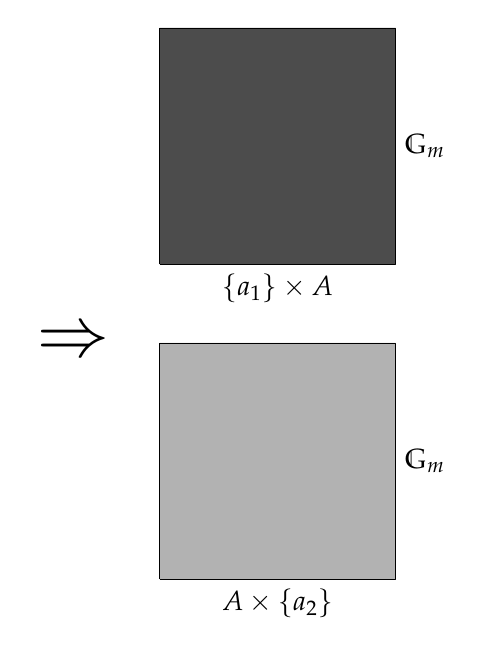
\begin{tikzpicture}
    \draw[very thin,black,line join=round,fill=black!30]
        (0,1) -- node [below,black] {$A \times \{a_2\}$} (3,1) -- node[right,black] {$\Gm$} (3,4) -- (0,4) -- (0,1);
    \draw[very thin,black,line join=round,fill=black!70]
        (0,5) -- node [below,black] {$\{a_1\} \times A$} (3,5) -- node[right,black] {$\Gm$} (3,8) -- (0,8) -- (0,5);
    \node[anchor=east] at (-0.5,4) {\Huge $\Rightarrow$};
\end{tikzpicture}
\end{center}
\caption{Extensions contained in a biextension.}
\end{figure}
There is a canonical piece of gluing data on this biextension, in the form of an isomorphism of pullback bundles
\begin{align*}
e_{p^j}\co (p^j \times 1)^* \L|_{A[p^j] \times A[p^j]} & \cong (1 \times p^j)^* \L|_{A[p^j] \times A[p^j]}, \\
(\ell, x, y) & \mapsto \left(\ell \cdot \prod_{k=1}^{p^j-1} \frac{s(x, [k]x, y)}{s(x, [k]y, y)} \right).
\end{align*}
This function $e_{p^j}$ is called the \textit{($p^j${\th}) Weil pairing}.
\end{definition}

\begin{remark}
In the case that $A$ is an elliptic curve, this agrees with the usual definition of its ``Weil pairing''. % In the case of an elliptic curve, this lines up with more traditional definitions --- for instance, using the isogeny $n: C \to C$.  In the case of a \emph{complex} elliptic curve $\C / (1, \tau)$, this degenerates further to the assignment \[\left( \frac{a}{n}, \frac{b}{n} \tau \right) \mapsto \exp\left(-2\pi i \frac{ab}{n}\right).\]
\end{remark}

\begin{lemma}\citeme{AS, I guess}
The Weil pairings assemble into a total Weil pairing on the $p$--divisible group associated to $A$.  Together, the total Weil pairing is alternating and biexponential. \qed
\end{lemma}

We can use the same formula in the setting of a cubical structure on a line bundle over a finite height formal group $\G$ to produce the desired map \[e_*\co C^3(\G; \Gm) \to \InternalHom{FormalGroups}(\G^{\wedge 2}, \Gm).\]  In fact, this is the right map:
\begin{lemma}[{\cite[Theorem 4.2, Corollary 4.4]{AndoStrickland}}]
The square commutes (up to sign):
\begin{center}
\begin{tikzcd}
\Spec E_0 BU[6, \infty) \arrow{r} \arrow{d}{\Pi_3} & \Spec E_0 K(\Z, 3) \arrow{d}{b_*} \\
C^3(\CP^\infty_E; \mathbb G_m) \arrow{r}{e} & \Weil(\CP^\infty_E).
\end{tikzcd}
\end{center}
\end{lemma}
\begin{proof}[Proof sketch]
This is reasonably difficult.  The main points are to show that the restriction \[d_{p^j}\co BC_{p^j}^{\times 2} \xrightarrow{\beta \circ \mu} \OS{H\Z}{3} \to BU[6, \infty)\] can be expressed by the Weil pairing formula: \[d_{p^j} = \bigoplus_{k=1}^{p^j-1} \left((\L_1 - 1)(\L_1^{\otimes k} - 1)(\L_2 - 1) - (\L_1 - 1)(\L_2^{\otimes k} - 1)(\L_2 - 1)\right).\]  After this is accomplished, what's left is to use naturality properties of the adjoint construction to compute the clockwise and counterclockwise composites.
\end{proof}

This fills out the diagram we are considering.  We now assemble just enough exactness results:

\begin{lemma}[{\cite[Lemma 7.2]{AndoStrickland}}]
The map $\delta\co C^2 \to C^3$ is injective for $\CP^\infty_E$ a finite height formal group.
\end{lemma}
\begin{proof}
Being finite height means that the multiplication-by-$p$ map of $\CP^\infty_E$ is fppf--surjective.  The kernel of $\delta$ consists of maps alternating, biexponential maps $(\CP^\infty_E)^{\times 2} \to \Gm$.  By restricting such a map $f$ to \[f \co \CP^\infty_E[p^j] \times \CP^\infty_E \to \Gm,\] we can calculate \[f(x, p^j y) = f(p^j x, y) = f(0, y) = 1.\]  But since $p^j$ is surjective on $\CP^\infty_E$, every point on the right-hand side can be so written, so at every left-hand stage the map is trivial.  Finally, $\CP^\infty_E = \colim_j \CP^\infty_E[p^j]$, so this filtration is exhaustive and we conclude that the kernel is trivial.
\end{proof}

\begin{lemma}[{\cite[Lemma 7.3]{AndoStrickland}}]
In fact, the following sequence is exact \[0 \to C^2(\CP^\infty_E; \Gm) \xrightarrow\delta C^3(\CP^\infty_E; \Gm) \to \Weil(\CP^\infty_E).\]
\end{lemma}
\begin{proof}
This is hard work.  Breen's idea is to show that picking a preimage under $\delta$ is the same as picking a trivialization of the underlying symmetric biextension of the cubical structure.  Then (following Mumford), one shows that the underlying symmetric biextension is trivial exactly if the Weil pairing is trivial.\todo{You could put in references here. AS gives them.}
\end{proof}

Finally, the top row falls quickly:

\begin{lemma}[{\cite[Lemma 7.5]{AndoStrickland}}]
\todo{Remark: This proof also shows that the $E$--theory of $\OS{kU}{8}$ fits into a sexseq.}
The top row of the main diagram is a short exact sequence of group schemes.
\end{lemma}
\begin{proof}
This is easiest proved by considering the sequence of homology Hopf algebras instead.  Since the integral homology of $BSU$ and the $E$--homology of $\OS{H\Z}{3}$ are both free and even, the Atiyah--Hirzebruch spectral sequence for $E_* BU[6, \infty)$ collapses.
\end{proof}

\begin{corollary}
The map \[\Pi_3\co \Spec E_0 BU[6, \infty) \to C^3(\CP^\infty_E; \Gm)\] is an isomorphism, and the map \[e_*\co C^3(\CP^\infty_E; \Gm) \to \InternalHom{FormalGroups}((\CP^\infty_E)^{\wedge 2}, \Gm)\] is a surjection.
\end{corollary}
\begin{proof}
This is a direct consequence of the $5$--lemma.
\end{proof}








% We begin with the fiber:

% \begin{lemma}[{\cite[Lemma 4.5]{AndoStrickland}}]\label{EasyCompatibilityWithdn}
% Write
% \begin{align*}
% d_n(\L_1, \L_2) & := \sum_{k=1}^{p^j-1} \left( (\L_1 - 1)(\L_1^k - 1)(\L_2 - 1) - (\L_1 - 1)(\L_2^k - 1)(\L_2 - 1)\right).
% \end{align*}
% There is a unique $\lambda \in \Z/n$ such that the following triangle commutes:
% \begin{center}
% \begin{tikzcd}
% (B\Z/p^j)^{\times 2} \arrow{d}{\lambda \beta \mu} \arrow{rd}{d_n(\L_1, \L_2)} \\
% K(\Z, 3) \arrow{r}{i} & BU[6, \infty).
% \end{tikzcd}
% \end{center}
% \end{lemma}
% \begin{proof}
% Forgetting down to $BU$ and working with just virtual bundles rather than lifts of virtual bundles to elements of $kU^6$, the definition of $d_n(\L_1, \L_2)$ gives
% \begin{align*}
% d_n(\L_1, \L_2) & = (\L_1 - 1)(\L_2^{p^j} - 1) - (\L_1^{p^k} - 1)(\L_2 - 1).
% \end{align*}
% Since we have restricted to $(B\Z/p^j)^{\times 2}$, $\L_1^{p^k} = 1$ and $\L_2^{p^k} = 1$, so this formula collapses and the composite map \[(B\Z/p^j)^{\times 2} \xrightarrow{d_n} BU[6, \infty) \xrightarrow{\pi_2} BSU \xrightarrow{\pi_2} BU\] is null.  We now study the lifting problem across the two maps:
% \begin{enumerate}
% \item[$\pi_1$:] Since the long composite is null, it follows that the shorter composite $\pi_2 \circ d_n$ factors through the fiber of $\pi_2$.  But, the fiber of $\pi_2$ is $S^1$, and there are no maps \[\{(B\Z/p^j)^{\times 2} \to S^1\} \cong H^1((B\Z/p^j)^{\times 2}; \Z) = 0.\]  It follows that $\pi_2 \circ d_n$ is itself null.
% \item[$\pi_2$:] Since $\pi_2 \circ d_n$ is null, $d_n$ must factor through the fiber of $\pi_2$, which is $K(\Z, 3)$.  With identical motives, one considers $H^3((B\Z/p^j)^{\times 2}; \Z)$, which is cyclic of order $n$ and generated by $\beta \circ \mu$. \qedhere
% \end{enumerate}
% \end{proof}

% \noindent This Lemma was missing a nontriviality statement, which turns out to be much harder:\todo{You could probably abbreviate the proof of this and include it.}

% \begin{theorem}[{\cite[Theorem 4.2, Section 5]{AndoStrickland}}]
% The value of $\lambda$ in \Cref{EasyCompatibilityWithdn} can be taken to be $\pm 1$. \qed
% \end{theorem}

% We now play one of our main cards: our willingness to work with cooperations means that we can pass from the hard task of checking facts about our formal schemes to the generally easier task of checking facts about their Cartier duals.  Because the formal schemes themselves are designed to have universal properties, their Cartier duals have points which are specified by these universal properties, and we win a considerable increase in tangibility.  In order to make full use of this, we record a mechanism of translation between these perspectives:


% These ideas power the following Lemma:

% \begin{proof}
% The target scheme $\Weil(\CP^\infty_E)$ is a subscheme of $\InternalHom{FormalGroups}((\CP^\infty_E)^{\times 2}, \Gm)$.  Since $\CP^\infty_E$ is finite height it satisfies $\CP^\infty_E = \colim_j \CP^\infty_E[p^j]$, which, coupled with the exponential adjunciton, reduces us to showing the agreement of the pair of composite maps \[\Spec E_0 BU[6, \infty) \times_{\S_E} \CP^\infty_E[p^j]^{\times 2} \to \Gm.\]  We will express these maps in terms of the adjoint map construction, starting with the clockwise composite.  The class $\beta \mu \in H\Z^3 BC_{p^j}^{\times 2}$ gives rise to an adjoint map \[\widehat{\beta \mu}\co \G_E[p^j]^{\times 2} \times (\OS{H\Z}{3})_E^\vee \to \Gm,\] which pulls back along $i\co \OS{H\Z}{3} \to \OS{kU}{6}$ to give \[(1 \times \Spec E_0 i) \circ \widehat{\beta \mu} = \widehat{i \beta \mu} = \widehat{d_n(\L_1, \L_2)}\] by the previous Theorem.

% We now try to calculate this adjoint, which will lead us to the counterclockwise composite.  First, the bundle $\bigotimes_{j=1}^3 (\L_j - 1) \in kU^6 (\CP^\infty)^{\times 3}$ gives rise to an adjoint map satisfying the following compatibility:
% \begin{center}
% \begin{tikzcd}
% (\CP^\infty_E)^{\times 3} \times \Spec E_0 BU[6, \infty) \arrow["\widehat{\bigotimes_{j=1}^3 (\L_j - 1)}"]{r} \arrow{d} & \Gm \\
% (\CP^\infty_E)^{\times 3} \times C^3(\CP^\infty_E; \Gm) \arrow{r} & (\CP^\infty_E)^{\times 3} \times \InternalHom{FormalSchemes}((\CP^\infty_E)^{\times 3}, \Gm) \arrow["\text{eval}"]{u}.
% \end{tikzcd}
% \end{center}
% The effect of postcomposing with the Weil pairing map can be viewed instead as precomposing the bottom-right corner with the






% \todo[inline]{This proof is unclear to the point of being broken.  How does the middle paragraph address the bottom-left arm of the square?}
% We will check compatibility on $\Weil_n(\CP^\infty_E)$ for arbitrary $n$, and so restrict from $i$ to $i \circ \lambda \beta \mu = d_n(\L_1, \L_2)$.
% % (Note: the sign can't bounce with $n$ because $\CP^\infty_E$ is $p$--divisible.)
% Since $\Weil_n(\CP^\infty_E)$ is a subscheme \[\Weil_n(\CP^\infty_E) \subseteq \InternalHom{FormalSchemes}(\CP^\infty_E[n]^{\times 2}, \Gm),\] we can push forward to checking equality here, i.e., of the two maps \[\Spec E_0 BU[6, \infty) \times_{\S_E} \CP^\infty_E[n]^{\times 2} \to \Gm.\]

% Writing $z = \prod_{i=1}^3 (1 - \L_i) \in kU^6 (\CP^\infty)^{\times 3}$, properties of the adjoint construction $\hat z$ show that it is given by the composite \[\hat z \co \Spec E_0 BU[6, \infty) \times_{\S_E} (\CP^\infty_E)^{\times 3} \to C^3(\CP^\infty_E; \Gm) \times_{\S_E} (\CP^\infty_E)^{\times 3} \xrightarrow{\operatorname{eval}} \Gm.\]  By specializing to $z = (1 - \L_1)(1 - \L_1^k)(1 - \L_2) \in kU^6 (\CP^\infty)^{\times 2}$, we see that $\hat z$ acts by\todo{Do I mean to be writing $k$--series here? I think I do.} \[\hat z \co (f, (g_1, g_2)) \mapsto f(g_1, [k](g_1), g_2),\] and continuing along these lines we see \[\widehat{d_n(\L_1, \L_2)} \co (f, (g_1, g_2)) \mapsto \prod_{k=1}^{n-1} \frac{f(g_1, [k](g_1), g_2)}{f(g_1, [k](g_2), g_2)} = e_n(f)(g_1, g_2).\]

% That described the bottom-left arm of the square.  The other way around the square is easier: take $w = \beta \circ \mu \in H^3(B\Z/p^j)^{\times 2}$ with adjoint $\hat w \co \CP^\infty_E[p^j]^{\times 2} \times K(\Z, 3)^E \to \Gm$.  Naturality shows $\hat w \circ \gamma^E = \widehat{\gamma_* w}$, and the theorem shows $\gamma_* w = \pm d_n(\L_1, \L_2)$, hence $\widehat{\gamma_* w} = (\pm d_n(\L_1, \L_2))\hat{}$, which is adjoint to $(e_n \Pi_3)^\pm$.
% \end{proof}

% \todo{There's a nice construction of the $\Pi_k$ maps in the AHS preprint where the ``$C_k$'' constructions are performed directly on the spectra, then applying $(-)_E$ carries those constructions to relevant constructions on group schemes, and finally Cartier duality gives the maps $\Pi_k$ of the sort described above.  This is superior to saying ``adjoint'', in my opinion, though it could be remarked that these are equivalent.}
% \todo{Consider including Lemma 6.2 and so on, the $BSU \to BU$ equivalents of the later statements you need.}

% % \begin{lemma}[{\cite[Lemma 6.2]{AndoStrickland}}]
% % The adjoint of the map $E_0 \CP^\infty \to E_0 BU$ induces a map $\Pi_1: BU^E \to C^1(\CP^\infty_E; \mathbb G_m)$ which is an isomorphism.  In fact, the Cartier duality isomorphism $(\CP^\infty)^E \cong \InternalHom{FormalGroups}(\CP^\infty_E, \mathbb G_m)$ fits into a commuting square
% % \begin{center}
% % \begin{tikzcd}
% % (\CP^\infty)^E \arrow{r} \arrow{d} & \InternalHom{FormalGroups}(\CP^\infty_E, \Gm) \arrow{d}{\begin{array}{c} \text{natural} \\ \text{inclusion} \end{array}} \\
% % BU^E \arrow{r}{\Pi_1} & C^1(\CP^\infty_E; \Gm).
% % \end{tikzcd}
% % \end{center}
% % \end{lemma}
% % \begin{proof}
% % \todo{Include this.}
% % \end{proof}

% % \begin{theorem}\label{BUBSUandC1C2Commute}
% % The following square commutes:
% % \begin{center}
% % \begin{tikzcd}
% % BU^E \arrow{d}{\Pi_1} \arrow{r} & BSU^E \arrow{d}{\Pi_2} \\
% % C^1(\CP^\infty_E; \Gm) \arrow{r}{\delta} & C^2(\CP^\infty_E; \Gm).
% % \end{tikzcd}
% % \end{center}
% % \end{theorem}
% % \begin{proof}
% % \citeme{Lemma 6.4 of AS}
% % This is a matter of expanding definitions and using \[(\L_1 - 1)(\L_2 - 1) = \mu^*(\L - 1) - \pi_1^*(\L - 1) - \pi_2(\L - 1).\]
% % \end{proof}

% % \begin{theorem}
% % The following is a map of short exact sequences:
% % \begin{center}
% % \begin{tikzcd}
% % 0 \arrow{r} & (\CP^\infty)^E \arrow{d} \arrow{r} & BU^E \arrow{r} \arrow{d} & BSU^E \arrow{r} \arrow{d} & 0 \\
% % 0 \arrow{r} & \InternalHom{FormalGroups}(\CP^\infty_E; \Gm) \arrow{r} & C^1(\CP^\infty; \Gm) \arrow{r} & C^2(\CP^\infty; \Gm) \arrow{r} & 0.
% % \end{tikzcd}
% % \end{center}
% % \end{theorem}
% % \begin{proof}
% % \citeme{Prop 6.5 of AS. They reference a superior alternate argument in the AHS preprint though\ldots}
% % \end{proof}








\section{Unstable additive cooperations for $kU$}

Write $H = H\F_p$.  Today we will study the effect of the map $\hat \Pi_3$ in ordinary homology.  Many parts of the proof we explored for $E$--theory break.  Topologically, the Serre spectral sequence for $H^* BU[6, \infty)$ is not even-concentrated and so is not forced to collapse.  Algebraically, because $\G_a$ is not $p$--divisible the behavior of the model exact sequence is also suspect.  Because the situation has fewer insulating good properties, we are forced to actually consider it carefully.  The upside, however, is that the standard group law on $\G_a$ is simple enough that we can compute the problem to death.

We begin with the topological half of our tasks.  The Serre spectral sequence \[E_2^{*, *} = H\F_p^* BSU \otimes H\F_p^* \OS{H\Z}{3}) \Rightarrow H\F_p^* BU[6, \infty)\] is quite accessible, and we will recount the case of $p = 2$.  In this case, the spectral sequence has $E_2$--page \[E_2^{*, *} = H\F_2^* BSU \otimes H\F_2^* \OS{H\Z}{3} \cong \F_2[c_2, c_3, \ldots] \otimes \F_2\left[\Sq^I \iota_3 \middle| \begin{array}{c} I_j \ge 2I_{j+1}, \\ 2 I_1 - I_+ \end{array}\right].\]  Because the target is $6$--connective, we must have the transgressive differential $d_4 \iota_3 = c_2$, which via the Kudo transgression theorem spurs the much larger family of differentials \[d_{4+I_+} \Sq^I \iota_3 = \Sq^I c_2.\]  This necessitates understanding the action of the Steenrod operations on the cohomology of $BSU$, which is due to Wu\citeme{Wu formulas, maybe May's concise book}:\todo{Can these formulas be read off from the divisorial calculation?  Maybe not, since it's easy to read off the Milnor primitives but harder to see the Steenrod squares.} \[\Sq^{2^j} \cdots \Sq^4 \Sq^2 c_2 = c_{1 + 2^j}.\]  Accounting for the squares of classes left behind, this culminates in the following calculation:\todo{This spectral sequence can be drawn in using Hood's package.}

\begin{theorem}\label{HF2BU6Calculation}
There is an isomorphism \[H\F_2^* BU[6, \infty) \cong \frac{H\F_2^* BU}{(c_j \mid j \ne 2^k + 1, j \ge 3)} \otimes F_2[\iota_3^2, (\Sq^2 \iota_3)^2, \ldots]. \qed\]
\end{theorem}

\begin{theorem}\citeme{Stong, Singer}
More generally, there is an isomorphism \[H\F_2^* \OS{kU}{2k} \cong \frac{H\F_2^* BU}{(c_j \mid \sigma_2(j - 1) < k - 1)} \otimes \operatorname{Op}[\Sq^3 \iota_{2k-1}],\] where $\sigma_2$ is the dyadic digital sum and ``$\operatorname{Op}$'' denotes the subalgebra of $H\F_2^* \OS{H\Z}{2k-1}$ generated by the indicated class.
\end{theorem}
\begin{proof}[Remarks on proof]
Stong specialized to $p = 2$ and carefully applied the Serre spectral sequence to the fibrations \[\OS{kU}{2(k+1)} \to \OS{kU}{2k} \to \OS{H\Z}{2k}.\]  Singer worked at an arbitrary prime and used the Eilenberg--Moore spectral sequence for the fibrations \[\OS{H\Z}{2k-1} \to \OS{kU}{2(k+1)} \to \OS{kU}{2k}.\]  Both used considerable knowledge of the interaction of these spectral sequences with the Steenrod algebra.
\end{proof}

\begin{remark}
These methods and results generalize directly to odd primes.  The necessary modifications come from understanding the unstable mod--$p$ Steenrod algebra, using the analogues of Wu's formulas due to Shay\citeme{Wu formulas, Shay's extension in \textit{mod--$p$ Wu formulas for the Steenrod algebra and the Dyer--Lashof algebra}}, and employing Singer's Eilenberg--Moore calculation.  Again, $H\F_p^* BU[6, \infty)$ is presented as a quotient by $H\F_p^* BU$ by certain Chern classes satisfying a $p$--adic sum condition, tensored up with the subalgebra of $H\F_p^* \OS{H\Z}{3}$ generated by a certain element.
\end{remark}

\begin{remark}
We can already see from \Cref{HF2BU6Calculation} that our map of short exact sequences in \Cref{ChromaticKUCoopnsSection} does not have a full analogue in the setting of additive homology.  By considering the edge homomorphism in the Serre spectral sequence, we see that \[\Spec HP_0 BSU \to \Spec HP_0 BU[6, \infty)\] is not a monomorphism.
\end{remark}





Now, we turn to the algebra.  The main idea, as already used in \Cref{CalculationOfLTTangentSpace}, is to first perform a tangent space calculation of \[T_0 C^k(\G_a; \Gm) \cong C^k(\G_a; \G_a),\] then study the behavior of the different tangent directions to determine the full object $C^k(\G_a; \Gm)$.  As a warm-up, we will first consider the case $k = 2$:
\begin{corollary}[{cf.\ \Cref{CohomologyOfGa}}]
The unique symmetric $2$--cocycle of homogeneous degree $n$ has the form \[c_n(x, y) = \begin{cases} (x + y)^n - x^n - y^n & \text{if $n \ne p^j$}, \\ \frac{1}{p} \left( (x + y)^n - x^n - y^n \right) & \text{if $n = p^j$}. \end{cases} \qed\]
\end{corollary}

Our goal, then, is to select such a $2$--cocycle $f$ and study the minimal conditions needed on a symbol $a$ to produce a multiplicative $2$--cocycle of the form $1 + af + \cdots$.  Since $c_n = \frac{1}{d_n} \delta(x^n)$ is itself produced by an additive formula, life would be easiest if we had access to an exponential, so that we could build \[\text{``$ \delta \exp(a_n x^n)^{1/d_n} = \exp(\delta a_n x^n / d_n) = \exp(a_n c_n). $''}\]  However, the existence of an exponential series is equivalent to requiring that $a_n$ have all fractions, which turns out not to be minimal.  In fact, \emph{no} conditions on $a_n$ are required \emph{at all}, if we tweak the definition of an exponential series:

\begin{definition}\todo{Where does this come from? I've never learned a universal property for it. That bothers me. It must have something to do with $p$--typification.}
The \textit{Artin--Hasse exponential} is the power series \[E_p(t) = \exp\left( \sum_{j=0}^\infty \frac{t^{p^j}}{p^j} \right) \in \Z_{(p)}\ps{t}.\]
\end{definition}

This series has excellent properties, mimicking those of $\exp(t)$ as closely as possible while keeping coefficients in $\Z_{(p)}$ rather than in $\Q$.  Writing $\delta\co C^1 \to C^2$ and \[d_n = \begin{cases} 1 & \text{if $n = p^j$}, \\ 0 & \text{otherwise}, \end{cases}\] we set \[g_n(x, y) := \delta E_p(a_n x^n)^{1/p^{d_n}} = \exp\left( \sum_{j=0}^\infty \frac{a_n^{p^j} \delta x^{np^j}}{p^{j + d_n}} \right) = \exp\left( \sum_{j=0}^\infty \frac{a_n^{p^j} c_{np^j}(x, y)}{p^j} \right).\]  This gives a point in $C^2(\G_a; \Gm)(\Z_{(p)}[a_n])$, and exhaustion of the tangent space proves the following Lemma:

\begin{lemma}[{\cite[Proposition 3.9]{AHSTheoremOfTheCube}}]
The map \[\Spec \Z_{(p)}[a_n \mid n \ge 2] \xrightarrow{\prod_{n \ge 2} g_2} C^2(\G_a; \Gm) \times \Spec \Z_{(p)}\] is an isomorphism. \qed
\end{lemma}

The case $k = 3$ is similar, with one important new wrinkle.  Over an $\F_2$--algebra there is an equality $c_n^2 = c_{2n}$.  However, this relation does not generalize to trivariate $2$--cocycles:
\begin{align*}
\frac{1}{2} \delta (c_6) & = x^2 y^2 z^2 + x^4 y z + x y^4 z + x y z^4, &
\left(\frac{1}{2} \delta c_3\right)^2 & = x^2 y^2 z^2.
\end{align*}
This pattern is generic and exhaustive for $\F_p$--algebras:
\begin{lemma}[{\cite[Proposition 3.20, Proposition A.12]{AHSTheoremOfTheCube}}]
The $p$--primary residue of the scheme of trivariate symmetric $2$--cocycles is presented by \[\Spec \F_p[a_d \mid d \ge 3] \times \Spec \F_p[b_d \mid d = p^j(1 + p^k)] \xrightarrow{\cong} C^3(\G_a; \G_a) \times \Spec \F_p. \qed\]
\end{lemma}

\noindent Similar juggling of the Artin--Hasse exponential yields the following multiplicative classification:
\begin{theorem}[{\cite[Proposition 3.28]{AHSTheoremOfTheCube}}]
There is an isomorphism \[\Spec \Z_{(p)}[a_d \mid d \ge 3, d \ne 1 + p^t] \times \Spec \Gamma[b_{1 + p^t}] \xrightarrow{} C^3(\G_a; \Gm) \times \Spec \Z_{(p)}.\]
\end{theorem}
\begin{proof}[Proof sketch]
The main claim is that the Artin--Hasse exponential trick used in the case $k = 2$ works here as well, provided $d \ne 1 + p^t$ so that taking an appropriate $p${\th} root works out.  They then show that the remaining exceptional cases extend to multiplicative cocycles only when the $p${\th} power of the leading coefficient vanishes.  Finally, a rational calculation shows how to bind these truncated generators together into a divided power algebra.
\end{proof}

In our pursuit of the map of exact sequences of \Cref{ChromaticKUCoopnsSection}, we are missing one piece: a link from topology to the scheme of Weil pairings, $\Weil(\G_a)$.  The object ``$\Spec HP_0 \OS{H\Z}{3}$'' is insuitable because it doesn't exist --- the homology algebra $HP_0 \OS{H\Z}{3}$ is not even--concentrated.  However, analyzing the edge homomorphism from our governing Serre spectral sequence shows that the map \[HP^0 BU[6, \infty) \to HP^0 \OS{H\Z}{3}\] factors through the subalgebra $A$ generated by the \emph{squares} of the polynomial generators.  Accordingly, we aim to place $\Spec A^*$ in the top-right corner of our map of 

\begin{lemma}[{\cite[Lemma 3.36, Proposition 4.13, Lemma 4.11]{AHSTheoremOfTheCube}}]
The scheme $\Spec A^*$ models $\Weil(\G_a)$ by an isomorphism $\lambda$ commuting with $e \circ \hat \Pi_3$.
\end{lemma}
\begin{proof}[Proof sketch]
The $\F_p$--scheme $\Weil(\G_a)$ is simple to describe:
\begin{center}
\begin{tikzcd}[row sep=1em]
(a_{mn})_{m, n} \arrow[|->]{r} & \prod_{m < n} \operatorname{texp}\left(a_{mn}(x^{p^m} y^{p^n} - x^{p^n} y^{p^m})\right) \\
\Spec \F_p[a_{mn} \mid m < n] / (a_{mn}^p) \arrow{r}{\cong} & \Weil(\G_a),
\end{tikzcd}
\end{center}
where $\operatorname{texp}(t) = \sum_{j=0}^{p-1} t^j / j!$ is the truncated exponential series.  It is easy to check that this ring of functions agrees with $A^*$, and it requires hard work (although not much creativity) to check the remainder of the statement: that $e \circ \hat \Pi_3$ factors through $\Spec A^*$ and that the factorization is an isomorphism.
\end{proof}

We have now finally assembled our map of right-exact sequences:\todo{It's maybe not obvious to a reader why this sequence is exact in the middle, although you have secretly proven this in the mess above.}
\begin{center}
\begin{tikzcd}
\Spec HP_0 BSU \arrow{r} \arrow["\hat \Pi_2", "\cong"']{d} & \Spec HP_0 BU[6, \infty) \arrow{r} \arrow["\hat \Pi_3"]{d} & \Spec A^* \arrow{r} \arrow["\lambda", "\cong"']{d} & 0 \\
C^2(\G_a; \Gm) \arrow{r}{\delta} & C^3(\G_a; \Gm) \arrow{r}{e} & \Weil(\G_a) \arrow{r} & 0.
\end{tikzcd}
\end{center}
Our calculations now pay off:
\begin{corollary}
The map $\hat \Pi_3$ is an isomorphism: \[\hat \Pi_3\co \Spec HP_0 BU[6, \infty) \xrightarrow{\cong} C^3(\G_a; \Gm).\]
\end{corollary}
\begin{proof}[Proof sketch]
The main point is that we don't actually have to compute much about the middle map.  Because the squares commute and the sequences are exact as indicated, we at least learn that $\hat \Pi_3$ is an epimorphism after base-change to $\Spec \Q$ and $\Spec \F_p$ for each prime $p$.  But, since both source and target are affine schemes of graded finite type with equal Poincar\'e series in each case, our epimorphism is an isomorphism.
\end{proof}

\begin{corollary}[{\cite[Theorem 2.31]{AHSTheoremOfTheCube}}]\label{Pi3ForCplxOrientableE}
The map $\hat \Pi_3$ is an isomorphism for any complex-orientable $E$.
\end{corollary}
\begin{proof}[Proof sketch]
This follows much along the lines of \Cref{HopfRingForEBP}.  We check that the statement holds for $E = MUP$ using a tangent space argument, and then an Atiyah--Hirzebruch argument gives the statement for any complex-oriented $E$.
\end{proof}


\begin{remark}
Our analysis in \Cref{LEFTCooperations} gives us full access to the Hopf ring structure of the \emph{nonconnective} cooperations $H\F_p{}_* \OS{KU}{2*}$.  Using a variety of techniques, Cowen Morton and Strickland calculated the Hopf ring structure of $H\F_2{}_* \OS{K}{2*}$ where $K$ ranges among the nonconnective objects $KO$, $KU$, $KSp$, and the less common ``$KT$'', which is self--conjugated $K$--theory~\cite{CowenMortonStrickland,StricklandBottPeriodicity}.
\end{remark}







\section{Covariance, $\Theta$--structures on Thom sheaves}

Today we will (despite appearances) mostly leave the algebraic geometry alone, instead attending to two lingering topological concerns.  First, over the past few lectures we have been concerned with the homology schemes $\Spec E_0 \OS{kU}{2*}$.  We were originally motivated by a sequence of cohomological isomorphisms
\begin{align*}
(BU \times \Z)_E & \cong \Sym^0_{\Div \CP^\infty_E} \Div_0 \CP^\infty_E =: C_0 \CP^\infty_E, \\
BU_E & \cong \Sym^1_{\Div \CP^\infty_E} \Div_0 \CP^\infty_E =: C_1 \CP^\infty_E, \\
BSU_E & \cong \Sym^2_{\Div \CP^\infty_E} \Div_0 \CP^\infty_E =: C_2 \CP^\infty_E,
\end{align*}
along with identifications
\begin{align*}
BU \times \Z & \simeq \OS{kU}{2 \cdot 0}, &
BU & \simeq \OS{kU}{2 \cdot 1}, &
BSU & \simeq \OS{kU}{2 \cdot 2}.
\end{align*}
Our analysis of Cartier duality in \Cref{TopologicalCartierDuality} gave us isomorphisms like \[\Spec E_0 BSU \cong \InternalHom{GroupSchemes}(BSU_E, \Gm) \cong \InternalHom{FormalGroups}(C_2 \CP^\infty_E, \G_m).\] Following the universal property of this particular symmetric square, we were led to consider the scheme of symmetric bivariate functions on $\CP^\infty_E$ satisfying a $2$--cocycle condition.  Our next move was to show that $\Spec E_0 BU[6, \infty)$ was modeled by a similar scheme of \emph{trivariate} functions --- but we proved this directly, while avoiding the ``predual'' cohomological statement \[BU[6, \infty)_E \cong C_3 \CP^\infty_E := \Sym^3_{\Div \CP^\infty_E} \Div_0 \CP^\infty_E.\]  This is because the homological statement is the low-hanging fruit: it is easy to demonstrate that the scheme of such functions exists as a closed subscheme of all functions.  It is considerably harder to show that a symmetric cube exists at all.

\begin{lemma}\label{CkGaGmAreFVars}\citeme{4.41 in the AHS preprint}
$C^k(\G_a; \Gm)$ are all formal varieties for $k \le 3$.
\end{lemma}
\begin{proof}
We will show that $\sheaf O(C^2(\G_a; \Gm))^*$ is a power series ring.  Because we know this ring to be torsion free, it suffices to show that it is a power series ring modulo $p$ for every prime $p$.  However, connected finite-type Hopf algebras over $\F_p$ were classified by Borel (and exposited in Milnor--Moore~\cite[Theorem 7.11]{MilnorMoore}) as either polynomial or truncated polynomial, so we are reduced to showing that $\sheaf O(C^2(\G_a; \Gm))^* \otimes \F_p$ is a graded polynomial ring.  These two cases are distinguished by the Frobenius operation: the Frobenius on a polynomial ring is injective, whereas the Frobenius on a truncated polynomial ring is not.  It is equivalent to show that the \emph{Verschiebung} on the original ring $\sheaf O(C^2(\G_a; \Gm)) \otimes \F_p$ is \emph{surjective}.  The equation $FV = p$, together with the observation $c_n^p = c_{np}$ of the level of bivariate $2$--cocycles, dictates the behavior of $V$: \[V(a_{np}) = a_n.\]

Essentially the same proof handles the cases $k = 1$ and $k = 0$.  The case $k = 3$ requires a small modification, to cope with the two classes of trivariate $2$--cocycles.  On the polynomial tensor factor of $\sheaf O(C^3(\G_a; \Gm))$ we can reuse the same Verschiebung argument to see that its dual Hopf algebra is polynomial.  The dual of the divided power tensor factor is immediately a primitively generated polynomial algebra, without any further argument.
\end{proof}

\begin{theorem}
The scheme $C_3 \CP^\infty_E$ exists, and it is modeled by $BU[6, \infty)_E$.
\end{theorem}
\begin{proof}[Proof sketch]
\citeme{Prop 3.3 in AHS preprint}
Let $\G$ be an arbitrary formal group.  Note first that if $C^3(\G; \Gm)$ is coalgebraic, then $C_3 \G$ exists and is its Cartier dual: the diagram presenting $\sheaf O(C^3(\G; \Gm))$ as a reflexive coequalizer of free Hopf algebras is also the diagram meant to present $C_3 \G$ as a coalgebraic formal scheme.  So, if the coequalizing Hopf algebra has a good basis, it will follow from \Cref{CoalgebraicColimitsExist} that the resulting diagram is a colimit diagram in formal schemes, with $C_3 \G$ sitting at the cone point.

\citeme{Prop 3.4 in the AHS preprint}
So, we reduce to checking that $\sheaf O(C^3(\G; \Gm))$ admits a good basis.  By a base change argument, it suffices to take $\G$ to be the universal formal group over the Lazard ring.  In this case, $\sheaf O(C^3(\G; \Gm))$ has graded\todo{Here we are again, making grading arguments. We've been bad about this earlier in the paper too.} finite type.  Specializing from $\G$ over $\moduli{fgl}$ to $\G_a$ over $\Spec \Z$, we know from \Cref{CkGaGmAreFVars} that $\sheaf O(C^3(\G_a; \Gm))$ is a free abelian group, and we know from \Cref{LazardsTheorem} that $\sheaf O(\moduli{fgl})$ is as well.  By picking a basis of each and a lift, we construct a free abelian group $M$ as well as a surjective map \[\alpha\co M \to \sheaf O(C^3(\G; \Gm)).\]  We proceed to test this map rationally: over $\Spec \Q$ we can use the logarithm to construct an isomorphism \[\Spec \Q \times (\moduli{fgl} \times C^k(\G; \Gm)) \to \Spec \Q \times (\moduli{fgl} \times C^k(\G_a; \Gm)),\] which shows that $\alpha \otimes \Q$ is an isomorphism.  By a finite type argument, this shows that $\alpha$ itself is an isomorphism, and we see further that $M$ has a sequence of good subcoalgebras spanned by the basis vectors of degree at most $d$.

Finally, it follows that the isomorphism $\Spec E_0 BU[6, \infty) \to C^3(\CP^\infty_E; \Gm)$ from \Cref{Pi3ForCplxOrientableE} re-dualizes to an isomorphism \[C_3 \CP^\infty_E \xrightarrow{\cong} BU[6, \infty)_E. \qedhere\]
\end{proof}

Our second task today is to address the gap between $\OS{kU}{2k}$ and its Thom spectrum $T(\OS{kU}{2k})$.  After all, our motivation for all of this algebraic geometry is to give a description to the set \[(\Spec E_0 MU[6, \infty))(E_0),\] but what we have done so far is describe the scheme $\Spec E_0 BU[6, \infty)$.  Since these two spectra are related by a Thom construction, we should be able to deduce the description that we want by thinking about Thom sheaves.  We now straighten this out.  The place to start is with a construction:

\begin{lemma}
For $\xi\co G \to BGL_1 \S$ a group map, the Thom spectrum $T\xi$ is a $(\Susp^\infty_+ G)$--cotorsor.
\end{lemma}
\begin{proof}[Proof sketch]
The Thom isomorphism $T\xi \sm T\xi \simeq T\xi \sm \Susp^\infty_+ G$ composes with the unit map $\S \to T\xi$ to give the \textit{Thom diagonal} \[T\xi \to T\xi \sm \Susp^\infty_+ G. \qedhere\]
\end{proof}

\begin{corollary}
In addition to our interpretation of $\ThomSheaf{\xi}$ as a $\Gm$--torsor over $G_E$, $\ThomSheaf{\xi}^{-1}$ is furthermore a $(G_E \times \Gm)$--torsor over $S_E$. \qed
\end{corollary}

We expand this idea out in our situation.  A morphism $MU[6, \infty) \to E$ produces a trivialization of $\ThomSheaf{\bigotimes_{j=1}^3 (\L_j - 1)}$ over $(\CP^\infty_E)^{\times 3}$, and the associated trivializing section is symmetric and rigid\citeme{Lemma 2.49 of AHS}.  This prompts us to make the following definition:

\begin{definition}
We write $C^k(\G; \sheaf L)$ for the functor of trivializing sections of $\Theta^k \sheaf L$ over $\G^{\times k}$ which are symmetric and rigid.  This construction has some nice properties:
\begin{itemize}
\item Note that taking the trivial sheaf $\sheaf L = \sheaf O_{\G}$ recovers the scheme $C^k(\G; \Gm)$ of $\Gm$--valued such functions from before.
\item By consequence, if $\sheaf L$ is \emph{trivializable} then this functor is an affine scheme.
\item Affine or not, there is a pairing map \[C^k(\G; \sheaf L) \times C^k(\G; \sheaf H) \to C^k(\G; \sheaf L \otimes \sheaf H).\]  In particular, this recovers the group structure on $C^k(\G; \Gm)$ and it makes $C^k(\G; \sheaf L)$ into a $C^k(\G; \Gm)$--torsor.
\end{itemize}
\end{definition}

\noindent Thus, we have constructed a map \[\Spec E_0 MU[6, \infty) \to C^k(\CP^\infty_E; \sheaf I(0)).\] The following Lemma is a matter of fully expanding definitions:

\begin{lemma}[{\cite[Theorem 2.50]{AHSTheoremOfTheCube}}]
The map \[\Spec E_0 MU[6, \infty) \to C^k(\CP^\infty_E; \sheaf I(0))\] is an isomorphism.
\end{lemma}
\begin{proof}
This map is equivariant, in the sense that the following square commutes:
\begin{center}
\begin{tikzcd}
\Spec E_0 MU[6, \infty) \times \Spec E_0 BU[6, \infty) \arrow{r} \arrow[equal]{d} & \Spec E_0 MU[6, \infty) \arrow[equal]{d} \\
C^k(\CP^\infty_E; \sheaf I(0)) \times C^k(\CP^\infty_E; \Gm) \arrow{r} & C^k(\CP^\infty_E; \sheaf I(0)).
\end{tikzcd}
\end{center}
Any equivariant map of torsors is automatically an isomorphism.
\end{proof}

\noindent This, finally, gives us access to the analogue of \Cref{BUZTriumvirate}, \Cref{BUTriumvirate}, and \Cref{BSUTriumvirate}:

\begin{corollary}\label{BU6Triumvirate}
Take $E$ to be \emph{complex--orientable}.  The functor $C^3(\CP^\infty_E; \sheaf I(0))$ defined by
\begin{align*}
\CatOf{AffineSchemes}_{/\Spec E_0} & \to \CatOf{Sets}, \\
(\Spec T \xrightarrow{u} \Spec E_0) & \mapsto \left\{ \begin{array}{c} \text{symmetric, rigid trivializations} \\ \text{of $u^* \Theta^3 \ThomSheaf{\L}$ over $u^* (\CP^\infty_E)^{\times 3}$} \end{array} \right\}
\end{align*}
is isomorphic to the affine scheme $\Spec E_0 MU[6, \infty)$.  Moreover, the $E_0$--points of this scheme biject with ring spectrum maps $MU[6, \infty) \to E$. \qed
\end{corollary}









\section{Elliptic spectra and Tate $K$--theory}

\begin{definition}
An \textit{elliptic spectrum} consists of:
\begin{enumerate}
\item An even-periodic ring spectrum $E$.
\item A (generalized) elliptic curve $C$ over $S_E$.\todo{I'm not sure if this is worth explaining. I guess we just mean elliptic curves with certain singularities allowed far away from the origin. Maybe it is worth explaining: you don't get examples like $H\Z P$ or $K^{\Tate}$ without allowing degeneracies.}
\item An isomorphism $\phi: C^\wedge_0 \cong \CP^\infty_E$.
\end{enumerate}
A \textit{map of elliptic spectra} consists of
\begin{enumerate}
\item A map of ring spectra $f: E \to E'$.
\item An \emph{isomorphism} of elliptic curves $f^* C \to C'$.
\end{enumerate}
\end{definition}

\todo{In particular, isogenies of elliptic curves are \emph{not} allowed. This is the realm of power operations.}

\begin{example}
Cohomology with complex coefficients and a selected lattice in the plane: $HP_\Lambda$.  The required isomorphism of formal groups comes from the logarithm map inverse to formally expanding $\C \to \C/\Lambda$ at the origin.
\end{example}

\begin{example}
Integral cohomology with the curve $zy^2 = x^3$.
\end{example}

\begin{example}
Ordinary $K$--theory with the curve $zy^2 + zxy = x^3$.
\end{example}

\begin{example}
Tate $K$--theory
\end{example}

\todo[inline]{I want to sketch the reduction for even-periodic elliptic cohomology theories to the case of $MUP$, then from there to $HkP$ for the prime fields $K$, then from there to questions about additive cocycles.  We certainly don't need to recall any of these calculations, but I think it's a nice example of the philosophy that the additive formal group is such a knotted point of $\moduli{fg}$ that it suffices to check something there to learn it for the rest of the stack.  This survives in the published form of AHS, but it's stated pretty clearly as Prop 3.4 in the unpublished verison.  See also 5.12 of the unpublished version.}

\todo[inline]{From the intro to the AHS preprint: For any lattice $\Lambda \subseteq \C$, we get a map $\Phi: MU[6, \infty) \to HP_\Lambda$ which sends $(2n)$--dimensional bordism classes $M$ to numbers $\Phi(M; \Lambda) \cdot u_{\Lambda}^n$. Suppose $\Lambda$ and $\Lambda'$ are two lattices with $\lambda \cdot \Lambda = \Lambda'$. This induces a map $HP_{\Lambda'} \to HP_\Lambda$ which intertwines the maps $\Phi$ by $\Phi(M; \lambda \cdot \Lambda) = \lambda^{-n} \Phi(M; \Lambda)$.  The usual appearance of a modular form (via $SL_2$ invariance) can be extracted from the top of page 5, if you want.  You can also show that this ``functional equation for a modular form'' is actually realized by a function by considering the elliptic cohomology theory built out of the bundle of elliptic curves $\mathfrak h \times \C/(1, \tau) \to \mathfrak h$ and the ordinary coefficient ring $\sheaf O[u^\pm]$, $\sheaf O$ the ring of holomorphic functions on $\mathfrak h$.}

-----------






\citeme{This part of the story is cribbed from AHS Section 2.6}
The other success of the $\theta$--functions story is that it gives access to a small piece of the compactified moduli of elliptic curves, $\overline{\moduli{ell}}$, called the Tate curve.  In this parametrized setting, define $D'$ to be the punctured complex disk, and set \[C'_{\mathrm{an}} = \C^\times \times D' / (u, q) \sim (qu, q).\]  The fiber of $C'$ over a particular point $q \in D'$ is the curve $\C^\times / q^{\Z}$ considered above, and $\theta$ determines a holomorphic function on the total space $\C^\times \times D'$.  The Weierstrass embeddings discussed above give an embedding of $C'_{\mathrm{an}}$ into $D' \times \CP^2$ described by \[wy^2 + wxy = x^3 - 5 \alpha_3 w^2 x + -\frac{5 \alpha_3 + 7 \alpha_5}{12}w^3\] for certain functions $\alpha_3$ and $\alpha_5$ of $q$.  At $q = 0$, these curve collapses to the twisted cubic \[wy^2 + wxy = x^3,\] and over the whole open unit disc $D$ we call this extended family $C_{\mathrm{an}}$.

Now let $A \subseteq \Z\ps{q}$ by the subring of power series which converge absolutely on the open unit disk.  It turns out that the coefficients of the Weierstrass cubic (i.e., $5\alpha_3$ and $\frac{1}{12}(5\alpha_3+7\alpha_5)$) lie in $A$, so it determines a generalized elliptic curve $C$ over $\Spec A$, and $C_{\mathrm{an}}$ is the curve given by base-change from $A$ to the ring of holomorphic functions on $D$.  The Tate curve $C_{\Tate}$ is defined to be the ``generalized elliptic curve'' over the intermediate object $D_{\Tate} = \Spec \Z\ps{q}$ as base-changed from $A$.  ``Generalized'' here means that the fiber over $q = 0$ is \emph{not} an elliptic curve --- but on its smooth locus it still carries the structure of a group scheme, and so one can still make sense of the associated formal group.

There are three natural coordinates available to us on $\widehat C_{\mathrm{an}}'$:
\begin{align*}
t & = x/y, &
\theta^{1/2,1/2}_q(u) & = \theta(t), &
1 - u & = 1 - u(t).
\end{align*}
Of these, only $t$ gives an algebraic coordinate on $C_{\mathrm{an}}'$ (and in fact on $C_{\mathrm{an}}$).  The others expand as power series in $t$ to
\begin{align*}
\theta(t) & = t + O(t^2), &
1 - u(t) & = t + O(t^2).
\end{align*}
The coefficients of the powers of $t$ in these series are holomorphic functions on the punctured disk $D'$.  In fact, they extend to $D$ and have integer coefficients\todo{... which you see by working over the completion of $\Z[u^pm]\ps{q}$ at $(1 - u)$}.  Thus $\theta(t)$ and $u(t)$ actually lie in $A\ps{t}$, so give functions on $\widehat C$ and $\widehat C_{\Tate}$.

Now, although $\theta^{1/2,1/2}_q$ does not give a section of $\sheaf I(0)$ on $C^3_{\mathrm{an}}$, it does descend to trivialize $\Theta^3 \sheaf I(0)$.  Then, since meromorphic sections of $\Theta^3 \sheaf I(0)$ on $C^3$ inject into such over $C_{an}^3$, the (transcendental) equation $s(C_{an}^3) = \delta^3 \theta^{1/2,1/2}_q(u)$ nonetheless determines the cubical structure on $\sheaf I(0)$ over $C$ and hence over $C_{\Tate}$ and $\widehat C_{\Tate}$ as well --- it can be expressed by $\delta^3 \theta(t)$.  It follows, finally, that the cubical structure extended over the compactification $D$ is also $\delta^3 \theta(t)$, since this function extends to $D$.\todo{Also, the invariant differential is $dx/(2y+x) = du/u$?}









Define the classical $\theta$--function on the Tate curve by \[\tilde \theta_q(u) = (1 - u) \prod_{n > 0} (1 - q^n u)(1 - q^nu^{-1}) \in \Z[u^{\pm}]\llbracket q \rrbracket.\]  Write $t = 1-u$ for the usual coordinate on the formal multiplicative group; then we can think of $\tilde \theta_q(u)$ as an element of $\Z\llbracket q\rrbracket\llbracket t\rrbracket$ and thus as a function on $\G_m \times D_{\Tate}$, $D_{\Tate} = \Spec \Z\llbracket t \rrbracket$ the Tate domain.  In fact, $\tilde\theta_q(u)$ is even a coordinate on this formal group over $D_{\Tate}$, which one can identify with $\widehat C_{\Tate}$.

By formal rearrangements one can produce the familiar functional equations
\begin{align*}
\tilde \theta_q(qu) & = -u^{-1} \tilde\theta_q(u), \\
\tilde \theta_q(q^k u) & = q^{-k(k-1)/2} (-u)^{-k} \tilde\theta_q(u).
\end{align*}
\todo{This is actually kind of hard to do algebraically. It's discussed in Appendix A of the AHS preprint.}
Regarding $\tilde\theta$ as an element of $C^0(\widehat C_{\Tate}; \L)$, this gives a cubical structure \[\delta^3(\tilde\theta) \in C^3(\widehat C_{\Tate}; \L),\] and one computes $\delta(\tilde\theta) = dt/\theta$ for \[\theta_q(u) = (1 - u) \prod_{n > 0} \frac{(1 - q^nu)(1 - q^n u^{-1})}{(1 - q^n)^2} \in \Z[u^\pm]\llbracket q \rrbracket,\] so you can also apply $\delta^2$ to this expression.\todo{Why would someone find this more familiar?  Also, in what sense is $\delta$ anything like differentiation?}  The functional equation has something to say about this cubical structure: \[(\delta^3 \tilde\theta_q)(u, v, w) = \begin{cases} (\delta^3 \tilde\theta_q)(qu, v, w), \\ (\delta^3 \tilde\theta_q)(u, qv, w), \\ (\delta^3 \tilde\theta_q)(u, v, qw). \end{cases}\]\todo{Mike has a nice remark about this: the exponents in the iterated functional equation for $\tilde\theta_q$ are quadratic in $k$ and so killed by $\delta^3$, which is another differentiation-type claim.}

\begin{theorem}\citeme{AHS preprint Prop 2.49}
The cubical structure $\delta^3(\tilde \theta)$ is the restriction of $s(C_{\Tate} / D_{\Tate})$ to $\widehat C_{\Tate}$.
\end{theorem}
\begin{proof}
The ratio $s(\widehat C_{\Tate} / D_{\Tate}) / \delta^3(\tilde\theta)$ is a power series $g \in \Z\llbracket q, t_0, t_1, t_2\rrbracket$ and we need to show that $g = 1$.  This will hold if we can show that there is a neighborhood of $0$ in $\C^4$ on which $g$ converges to $1$, so we can employ complex analytic techniques.  Fix $q \in \C$ with $0 < |q| < 1$ and let $C_q$ be the $\C$--analytic elliptic curve fibering over this point in $D_{\Tate} \times \Spec \C$.  The product expansion of $\tilde\theta_q(u)$ converges locally uniformly to an analytic function on $\C^\times$ vanishing only on $q^{\Z}$ and there only to first order.  It should suffice to show that $s(C_q/\C) = \delta^3(\tilde\theta_q)$ as analytic functions on $(\C^\times)^{\times 3}$.  The consequence for $\delta^3 \tilde\theta$ of the functional equation for $\tilde\theta$ recalled above shows that $\delta^3\tilde\theta_q$ descends to give a meromorphic $1$--form $\phi$ on $C_q^{\times 3}$.  Then, because $\tilde\theta_q$ has only simple poles on $q^{\Z}$ and none elsewhere, we deduce that $\phi$ is actually a cubical structure, and unicity then finally forces $\phi = s(C_q / \C)$.
\end{proof}

\todo[inline]{See also the bottom of page 22 in the AHS preprint for the relevant theory of integration (esp. Prop 2.54), and see Proposition 2.56 for a comparison theorem between the integration theory and $\sigma_{\Tate}$.}

\begin{definition}
Let $\gamma$ denote the element $K_{\Tate}(\Z \times BU)$ determined by the vector bundle operation \[\gamma: -V \mapsto \prod_{n > 0} \sum_{k \ge 0} q^{nk} \Sym^k(V),\] and let $\bar\gamma$ denote its complex conjuguate.  Since $K_{\Tate}^0(MUP)$ is a module over $K_{\Tate}(\Z \times BU)$, we can define an element \[\sigma_{\Tate} := \gamma \cdot \bar\gamma \cdot \alpha,\] where $\alpha$ is the usual orientation $MP \to KU$ corresponding to the coordinate $1 - t$ on the formal group $\G_m$.
\end{definition}

\todo{``Modularity'' of the $K_{\Tate}$ orientation?}


------------

Criteria for the existence of symmetric cocycle schemes.

AHS: they exist
\todo[inline]{The technical condition guaranteeing the existence of symmetric power schemes is that the symmetric cocycle schemes are coalgebraic formal schemes, since then we have an involutive Cartier duality functor.  This comparison essentially comes out of saying that $C_k$ can be defined by a strong colimit, so if we can check that this strong colimit exists\ldots (cf. Prop 3.3 of the AHS preprint).}

------------

Here's what the published version of AHS has to say about the $\sigma$--orientation of $K_{\Tate}$.  (See Section 2.7.)

$K_{\Tate}$ has multiplicative cohomology theory $K\ps{q}$, formal group multiplicative (as induced by $K$--theory), and isomorphism to $\widehat C_{\Tate}$ given by $1 - u(t)$ as in Lecture 5.2.  Since the cubical structure on $\widehat C_{\Tate}$ is given as $\delta^3$ of something, it follows that the $\sigma$--orientation factors as
\begin{center}
\begin{tikzcd}
MU[6, \infty) \arrow{d} \arrow{drr} \\
MU \arrow{r} & MUP \arrow{r}{\tilde \theta} & K\ps{q}.
\end{tikzcd}
\end{center}
Our goal is to express in terms of characteristic classes the induced map on homotopy by the horizontal composite.

To start with, the topological restriction $MU \to MUP \to E$ sends the coordinate $f$ on $\G_E$ to the rigid section $\delta f$ of $\Theta^1(\sheaf I(0)) = \sheaf I(0)_{0} \otimes \sheaf I(0)^{-1}$.  The most straightforward formula for $\delta f$ is $f(0) / f$, which is confusing, since $f(0) = 0$ usually but not as a section of $\sheaf I(0)_0$.  It's probably clearer to express $\delta f$ in terms of the isomorphism \[\sheaf I(0)_0 \otimes \sheaf I(0)^{-1} \cong \omega \otimes \sheaf I(0)^{-1},\] where $\delta f$ is given by the formula \[\delta f = \frac{f'(0) Dx}{f(x)},\] $Dx$ the invariant differential with value $dx$ at $0$.

In the example of $K$--theory, the usual complex Atiyah--Bott--Shapiro map $MP \to K$ corresponds to the coordinate $1 - u$ on the formal completion of $\Gm = \Spec \Z[u^\pm]$.  The invariant differential is $D(1 - u) = -du/u$, and the restriction to $MU$ classifies the $\Theta^1$--struucture \[\delta(1 - u) = \frac{1}{1 - u}\left(-\frac{du}{u}\right).\]  In the more complex example of Tate $K$--theory, the map \[MU \to MUP \xrightarrow{\tilde\theta} K_{\Tate}\] factors by the coordinate change map \[MU \to MU \sm MU \simeq MU \sm BU_+ \xrightarrow{\delta(1 - u) \sm \theta'} K_{\Tate},\] where $\theta'$ is the element of $BU^{K_{\Tate}} \cong C^1(\widehat C_{\Tate}; \Gm)$ given by the formula \[\theta' = \prod_{n \ge 1} \frac{(1 - q^n)^2}{(1 - q^n u)(1 - q^n u^{-1})}.\]

\needproof{The Todd genus}
In geometric terms, the homotopy groups $\pi_* MU \sm BU_+$ are the bordism groups of pairs $(M, V)$ consisting of a stably almost complex manifold $M$ and a virtual complex vector bundle $V$ over $M$ of virtual dimension $0$.  The map \[\pi_* MU \to \pi_* (MU \sm BU_+)\] sends a manifold $M$ to the pair $(M, \nu)$ where $\nu$ is the reduced stable normal bundle.  Next, the map $\pi_* \delta(1 - u)$ sends a manifold $M$ of dimension $2n$ to $p_!(1) \in K^{-2n}(*)$ where $p: M \to *$ is the unique map.  One has \[p_!(1) = \operatorname{Td}(M) \left( -\frac{du}{u} \right)^n,\] where $\operatorname{Td}(M)$ is the Todd genus of $M$ (and it is customary to suppress the grading and write $p_!(1) = \operatorname{Td}(M)$).  The map $\theta'$ is where the real work is: it is the stable exponential characteristic class taking the value \[\prod_{n \ge 1} \frac{(1 - q^n)^2}{(1 - q^n \L)(1 - q^n \L^{-1})}\] on the reduced class $(1 - \L)$ of a line bundle $\L$.  This stable exponential characteristic class can easily be identified with \[V \mapsto \bigotimes_{n \ge 1} \Sym_{q^n}(- \bar V_{\C}),\] where $V_{\C} = V \otimes_{\R} \C$, $\bar V_{\C} = V_{\C} - \eps^{\oplus \dim V}$, and $\Sym_t(W)$ is defined for (complex) vector bundles $W$ by \[\Sym_t(W) = \bigoplus_{m \ge 0} \Sym^m(V) t^m \in K(M)\ps{t}\] and extended to virtual bundles using the exponential rule $\Sym_t(W_1 - W_2) = \Sym_t(W_1) / \Sym_t(W_2)$.  Altogether, the effect of the $\sigma$--orientation therefore sends an almost complex manifold $M$ of dimension $2n$ to
\begin{align*}
\pi_* \sigma_{K_{\Tate}}(M) & = f_! \left( \bigotimes_{n \ge 1} \Sym_{q^n}(\bar T_{\C}) \right) \\
& = \operatorname{Td}\left(M; \bigotimes_{n \ge 1} \Sym_{q^n}(\bar T_{\C}) \right) \left( -\frac{du}{u} \right)^n \\
& \in \widetilde K\ps{q}^0(S^{2n}).
\end{align*}

This is basically Witten's formula for his genus.  There is a small caveat: Witten's genus is defined for Spin manifolds.  With some care, perhaps we could construct a homotopical square\todo{Is this possible?  Or do we really need the $\String$--orientation to make this happen?  Is this exactly the topic for the next day?!!}
\begin{center}
\begin{tikzcd}
MSU \arrow{r} \arrow{d} & MU \arrow{d} \\
M\Spin \arrow[densely dotted]{r} & K_{\Tate},
\end{tikzcd}
\end{center}
but for the moment we content ourselves with a square of homotopy groups
\begin{center}
\begin{tikzcd}
\pi_* MSU \arrow{r} \arrow{d} & \pi_* MU \arrow{d} \\
\pi_* M\Spin \arrow[densely dotted]{r} & \pi_* K_{\Tate}.
\end{tikzcd}
\end{center}
Let $M$ be a $\Spin$--manifold of dimension $2n$, and use the splitting principle to write \[TM = \L_1 \oplus \cdots \oplus \L_n\] for complex line bundles $\L_i$.  The $\Spin$--structure gives a square root of $\prod \L_i$, which is equivalent to picking a square root for each $\L_i$.\todo{Is it?}  Since, for each $i$, the $O(2)$--bundles underlying $\L_i^{1/2}$ and $\L_i^{-1/2}$ are isomorphic, we can write \[TM = \sum \L_i + \L_i^{-1/2} - \L_i^{1/2},\] which is now a sum of $SU$--bundles.  Using this, one easily checks that the $\sigma$--orientation of $M$ gives \[\widehat A \left(M; \bigotimes_{n \ge 1} \Sym_{q^n}(\bar T_{\C}) \right) \left(-\frac{du}{u}\right)^n,\] where the $\widehat A$--genus is the push-forward in $KO$--theory associated to the unique orientation $M\Spin \to KO$ fitting into the commutative diagram
\begin{center}
\begin{tikzcd}
MSU \arrow{r} \arrow{d} & MU \arrow{d} \\
M\Spin \arrow{rd} \arrow{r} & K \\
& KO \arrow{u}{\widehat A}.
\end{tikzcd}
\end{center}

Finally, we want to see that for $[M] \in \pi_{2n} MU[6, \infty)$, \[\Phi(M) := (\pi_{2n} \sigma_{K_{\Tate}})(M) \left( -\frac{du}{u} \right)^{-n} \in \pi_0 K_{\Tate} = Z\ps{q}\] is a modular form.  We've at least seen that $\Phi(M)$ is a holomorphic function on $D$, with integral $q$--expansion coefficients.  It suffices to show that if $\pi: \h \to D$ is the map $\pi(\tau) = e^{2 \pi i \tau}$, then $\pi^* \Phi(M)$ transforms correctly under the action of $SL_2(\Z)$.  This is supposed to follow from stuff in the introduction (pp.\ 600-1, also Example 2.3).


\todo[inline]{Now that you have an extra few days, you could actually go through the calculation of $H\F_{p*} \OS{ku}{2k}$ and $C^k(\G_a; \Gm)$.}






\section{$\Spin$ and $\String$ orientations}

Formal schemes for certain real $K$--theory spaces

The Atiyah--Bott--Shapiro orientation and the fibration $BSU \to BSpin$ \citeme{Theorem 2.3.5.iv in KLW, the last fibration in 2.3.2 at $k=-2$, and sections 5.3 and 5.13}

The $\String$ orientation and $\Sigma$--structures




The following definition is meant to curtail the behavior of Hopf algebras at the prime $p = 2$, where the erasure of signs can cause strange things to happen.  In particular, Hopf algebras satisfying the following condition split as the tensor product of an exterior odd--dimensional part and a commutative even--dimensional part.

\begin{definition}\citeme{KLW Remark 4.5}
A Hopf algebra is said to be \textit{Restriction A} when it is formed from the following components:
\begin{itemize}
\item A polynomial algebra on a single even--degree generator.
\item A truncated polynomial algebra on a single even--degree generator.
\item An algebra on a single even generator $x$ where a large power $x^{p^d}$ can be rewritten in terms of lower powers.
\item An exterior algebra on a single odd--degree generator.
\item A ``divisible algebra'' $P_\infty = k\<a_0, a_1, \ldots, a_n, \ldots\>$ where $a_n^p = a_{n-1}$ and $a_0^p = 0$. \todo{Pepper these with topological examples.}
\end{itemize}
\end{definition}

\begin{theorem}\citeme{Theorem 4.2 of KLW}
Let $F \xrightarrow i E \xrightarrow r B$ be a fibration of connected double loopspaces, let $K$ have K\"unneth isomorphisms, and let $K_* F$ be a bicommutative Hopf algebra.  Then there is a spectral sequence of Hopf algebras \[E^2_{*, *} = \Tor^{K_* F}_{*, *}(K_* E, K_*) = \Tor^{\ker i_*}_{*, *}(K_*, K_*) \otimes \coker i_* \Rightarrow K_* B,\] where $\coker i_* = \Tor^{K_* F}_{0, *}(K_* E, K_*)$.  If $i_*$ is injective, this gives a short exact sequence of Hopf algebras \[K_* \to K_* F \to K_* E \to K_* B \to K_*.\]  If $\ker i_*$ is Restriction A and $\coker i_*$ is even, then $\coker i_*$ injects into $K_* B$ and all differentials take place in $\Tor^{K_* F}_{*, *}(K_* K_*)$.  If \[\Loops F \to \Loops E \to \Loops B\] induces a short exact sequence of Hopf algebras on $K$--homology with $K_* \Loops B$ Restriction A and $K_* F$ even, then the original fiber sequence also induces a short exact sequence of Hopf algebras. \qed
\end{theorem}

\begin{corollary}\citeme{Theorem 4.4 of KLW}
Let $E \to B' \to B$ be connective coverings of a simply connected double loopspace $B$.  Consider the following diagram of fiber sequences:
\begin{center}
\begin{tikzcd}
F' \arrow{d} \arrow{r} & E \arrow[equal]{d} \arrow{r} & B' \arrow{d} \\
F \arrow{r} & E \arrow{r} & B.
\end{tikzcd}
\end{center}
If the bottom row induces a short exact sequence of Hopf algebras on $K$--homology, then so does the top row. \qed \todo{Maybe you could prove this. It relies on the finite Postnikov systems result which you may have talked about back in the Dieudonne modules sections.}
\end{corollary}

\todo{We mostly need to see that Postnikov sections induce short exact sequences.  For that, note that the $K$--theory of EM spaces is always Restriction A.}

\todo{Include a remark about Section 5.2 on ``Bicommutativity''.}





\begin{lemma}[{\cite[Lemma 2.1]{Yagita}}]
Let $\Gamma$ be a formal group over $k$ of height $\height{\Gamma} = d$, and let $k_\Gamma$ be the connective cover of the Morava $K$--theory $K_\Gamma$.  In the Atiyah--Hirzebruch spectral sequence \[E_2^{*, *} = Hk^* X \otimes_k k_\Gamma^* \Rightarrow k_\Gamma^* X,\] the differentials are given by \[d_r(x) = \begin{cases} 0 & \text{if $r \le 2(p^d - 1)$}, \\ \lambda Q_d x \otimes v_d & \text{if $r = 2(p^d - 1) + 1$} \end{cases}\] where $\lambda \ne 0$ and $Q_d$ is the $d${\th} Milnor primitive. \qed
\end{lemma}





\begin{theorem}
There is a bi-Cartesian square
\begin{center}
\begin{tikzcd}
& \Div_0 \overline{\G}[2] \arrow{rr} \arrow{ld} & & \Div_0 \G[2] \arrow{ld} \\
\Div_0 \overline{\G} \arrow{rr} & & BO_K.
\end{tikzcd}
\end{center}
\end{theorem}
\begin{proof}
\todo{Analyze the Atiyah--Hirzebruch spectral sequence}
\end{proof}

\begin{lemma}
Consider the cube constructed by taking pointwise fibers of the composite to $X$.
\begin{center}
\begin{tikzcd}
& A' \arrow{rr} \arrow{ld} \arrow{dd} & & B' \arrow{ld} \arrow{dd} \\
C' \arrow{rr} \arrow{dd} & & D' \arrow[crossing over]{dd} \\
& A \arrow{rr} \arrow{ld} & & B \arrow{ld} \\
C \arrow{rr} & & D \arrow{rr} & & X.
\end{tikzcd}
\end{center}
If the bottom face is bi-Cartesian, then so is the top.
\end{lemma}
\begin{proof}
\todo{Prove this? It's valid in an arbitrary abelian category.}
\end{proof}

\begin{corollary}
There is a bi-Cartesian square
\begin{center}
\begin{tikzcd}
& \Div_0 \overline{\G}[2] \arrow{rr} \arrow{ld} & & \SDiv_0 \G[2] \arrow{ld} \\
\Div_0 \overline{\G} \arrow{rr} & & BSO_K. & & \qed
\end{tikzcd}
\end{center}
\end{corollary}
\begin{proof}
\todo{Write this for real.}
The fibration $BSO \to BO \to BO(1)$ gives a short exact sequence of Hopf algebras.  The composite $\Div \overline{\G} \to \G[2]$ acts by zero and the composite $\Div \G[2] \to \G[2]$ acts by summation.  The summation one you can probably prove by comparing with the determinant (or Postnikov) section for $BU$.
\end{proof}

\begin{corollary}
\todo{Write this for real. Even the statement is bad: see ``$\ker \omega$''.}
There is a bi-Cartesian square
\begin{center}
\begin{tikzcd}
& \Div_0 \overline{\G}[2] \arrow{rr} \arrow{ld} & & \ker \omega \arrow{ld} \\
\Div_0 \overline{\G} \arrow{rr} & & B\Spin_K. & & \qed
\end{tikzcd}
\end{center}
\end{corollary}
\begin{proof}
This goes similarly to the one above.  You can compute that the composite $\Div \overline{\G} \to \G[2]^{\wedge 2}$ is zero using an identical technique.  To compute the action on the other factor, KLW show that there's a diagram of exact sequences
\begin{center}
\begin{tikzcd}
& & & K_* \arrow{d} \\
& & & K_* K(\Z, 3) \arrow{d} \\
K_* \arrow{r} & K_* B\Spin \arrow{r} \arrow{d} & K_* BSU \arrow{r}{\tau} \arrow[equal]{d} & K_* BU[6, \infty) \arrow{d}{\delta} \\
K_* \arrow{r} & K_* BSO \arrow{r}{i} & K_* BSU \arrow{r}{1 - \xi} & K_* BSU \arrow{d} \\
& & & K_* .
\end{tikzcd}
\end{center}
Since $(1 - \xi) \circ i = 0$, we have that $\delta \circ \tau \circ i = 0$ and hence that $\tau \circ i$ lifts to $K_* K(\Z, 3)$.  Identifying $\SDiv_0 \G[2]$ with $C_2 \G[2]$, we check that the composites \[C_2 \G[2] \xrightarrow{\omega} \G[2]^{\wedge 2} \xrightarrow{\eps} C_3 \G\] and \[C_2 \G[2] \to C_2 \G \xrightarrow{\tau} C_3 \G\] agree.  For a point $[a, b] \in C_2 \G$, this is the claim
\begin{align*}
0 & = \eps(a \wedge b) - \tau[a, b] \\
& = [a, a, b] - [b, a, b] - [-a - b, a, b] \\
& = [a, a, b] - [b + a, a, b] + [b, a + a, b] - [b, a, b],
\end{align*}
and this is the expression called $R(b, a, a, b)$, which is forced null in $C_3 \G$.

\todo[inline]{I'm a little fuzzy on the coherence of this with the Bockstein: this computes the lift of $\tau \circ f$ into $K(\Z, 3)_K$, and it does happen to factor through the subscheme $K(\Z/2, 2)_K$ determined by the Bockstein. However, I don't immediately see why this agrees with the bottom Postnikov section of $BSO$: that's a map off of $BSO$ and this is a rotated map into $BU[6, \infty)$, so it's not an immediate consequence of naturality.}
\end{proof}



\todo{What follows is the analysis for $M\String$.  Is the one for $M\Spin$ analogous and do-able?  Does it involve $CK_2$ and maybe a clever choice of $MSU$--orientation?}


The sequence $\Spin/SU \to BU[6, \infty) \to B\String$ is exact and right-exact.  The kernel of the map $\Spin/SU \to BU[6, \infty)$ is ``$CK_3$'' \citeme{Theorem 2.3.5.vi of KLW}, where \[CK_j = \bigoplus_{k=j}^\infty K_* K(\Z/2, k).\]  More than that, KLW even say where the polynomial and nonpolynomial parts of $K_* \Spin/SU$ land inside of $K_* BU[6, \infty)$.  I think\todo{But I have not checked!} that this means that $K_* BU[6, \infty)$ is a flat $K_* \Spin/SU$--module at heights $d \le 2$.

Anyway, there's always a $\Tor$--spectral sequence owing to the pushout diagram
\begin{center}
\begin{tikzcd}
\Susp^\infty_+ \Spin/SU \arrow{r} \arrow{d} & MU[6, \infty) \arrow{d} \\
* \arrow{r} & M\String
\end{tikzcd}
\end{center}
of signature \[\Tor^{K_* \Spin/SU}_{*, *}(K_* MU[6, \infty), K_*) \Rightarrow K_* M\String.\]  So, under the flatness hypothesis above, there are no higher $\Tor$ terms so the spectral sequence collapses to give \[K_* M\String \cong K_* MU[6, \infty) \mmod K_* \Spin/SU.\]  So, what remains to be shown is that $K_* \Spin/SU$ picks out the correct extra relation for $\Sigma$--structures.  Then, we need a density argument to show that this handles all of the at-a-point cases of elliptic cohomology.







-------

Some other things that might belong in this chapter:

The cubical structure on a singular (generalized) elliptic curve is not unique, but (published) AHS has an argument showing that the unicity of the choice on the nonsingular ``bulk'' extends to a unique choice on the ``boundary'' of the compactified moduli too.


There's also the work of Ando--French--Ganter on factorized / iterated $\Theta$ structures and how they give rise to the ``two--variable Jacobi genus''.














% -*- root: main.tex -*-

\chapter{Power operations}

\todo{I wish this had a better title.}

\todo{Write an introduction for me.}

\todo{Baker's POWER OPERATIONS AND COACTIONS IN HIGHLY COMMUTATIVE
HOMOLOGY THEORIES seems like a nice place to learn about these things. He advertises some interaction with the traditional context story, which is appealing, and he mostly treats the case of ordinary homology, which we probably ought to spend a section on.}

\todo{Charles's Sections 2.10,12 of the Felix Klein notes has a nice, compact exposition of power operations for $K(n)$--local $E_\infty$--ring spectra (using, in particular, $R^{B\Sigma_m} \simeq R \sm_E E^{B\Sigma_m}$) as well as a discussion of ``descent for isogenies'' generally and Koszul-ality in Section 3.}


\begin{center}
\textbf{\Large This is completely under construction.}
\end{center}


\todo[inline]{There should be a context-based presentation of this chapter's material too.  What do contexts for structured ring spectra look like?  Why would you consider them --- what object are you trying to approximate?  How do you guess that the algebraic model is reasonable until you're aware of something like Strickland's theorem?}

\todo[inline]{Since you spend so much time talking about descent in other parts of these notes, maybe you should also read the end of the AHS $H_\infty$ paper where they claim to recast their results in the usual language of descent.}

\todo[inline]{Conversation with Nat on 2/9 suggests taking the following route in this chapter:
contexts for $E_\infty$ mapping spaces in general;
Subgroups and level structures;
the Drinfel'd ring and the universal level structure;
the isogenies pile;
power operations and Adams operations, after Ando (naturally indexed vs indexed on subgroups; have a look at the Screenshot you took on this day);
comparison of comodules $M$ for the isogenies pile with the action of $M_n(\Z_p)$ on $M \otimes_{E_n^*} D_\infty$ (this is a modern result due to Tomer, Tobi, Lukas, and Nat);
$H_\infty$ $MU$--orientations and Matt's thesis;
the analogous results for $\Theta^k$--structures.
In particular, leave character theory, $p$--divisible groups, and rational phenomena for spillover at the end of the year. They aren't strictly necessary to telling the story; you just need to know a little about the Drinfel'd ring to construct Matt's maps.  (If you have time, though, the point is that the rationalized Drinfel'd ring carries the universal level structure which is also an isomorphism.)}

\todo[inline]{The stuff around 4.3.1-2 of Matt's published thesis talks about $H_\infty$--maps being determined by their values on $*$ and $\CP^\infty$, which is an interesting result.  You might also compare with Butowiez--Turner.}

\todo[inline]{Work in height $1$ (and height $2$??) examples through this?  $K$--theory is pretty accessible, and the height $2$ examples are somewhat understood (Charles, Yifei), and they're both relevant for the elliptic $M\String$ story.  (There's also the pile of elliptic curves with isogenies...)}

\todo[inline]{Nat warns that the very end of Matt's thesis uses character theory for $S^1$, which you have to be very careful about to pull off correctly.  ($S^1$ is not a finite group, but in certain contexts it can be approximated by its torsion subgroups...)}

\todo[inline]{Yifei warned me that Matt's ``there exists a unique coordinate...''\ Lemma is specifically about lifting the \emph{Honda} formal group law over $\F_q$.  If you want to do this with elliptic cohomology or something, then you need a stronger statement (and it's clear what this statement should be, but no one has proven it).}

\todo{This MO conversation looks interesting: http://chat.stackexchange.com/transcript/message/29465746\#29465746.}


------ Here are various notes from conversations with Nat, recorded and garbled well after they happened. ------

We could try to understand Matt's thesis's Section 4.2.  It identifies the action of the internal power operation on $E_n$ using the internal theory of quotient isogenies to the Lubin--Tate deformation problem (2.5.4).  Conditions 1 and 3 of 4.2.1 are easy to verify: they are 4.2.3 (evaluate on a point) and 4.2.4 (the power operation does raise things to a power) respectively.  Condition 2 takes more work, and it's about identifying the divisor associated to the isogeny granted by Condition 1.  It's worked out in 4.2.5, which is not very hard, and 4.2.6, which shows that \emph{the} Thom class associated to a vector bundle is sent under a power operation to \emph{some} Thom class.  4.2.5 then uses that the quotient of \emph{some} Thom classes has to be a unit in the underlying ring.

(Q: Can 4.2.5 be phrased about two coordinates on the same formal group, rather than two presentations of the same divisor?  There's a comparison between functions on the quotient with invariant functions on the original group --- and perhaps with functions invariant by pulling back along the isogeny?)

Prop 8.3 in ``Character of the Total Power Operation'' provides an algebro-geometric proof of something in AHS04, using the fact that for $R$ a nice complete local ring and $G$, $G'$ $p$--divisible groups over $R$, there is an injection \[\Isog_R(G, G') \into \Isog_{R/\m}(G, G').\]

Nat thinks that using the power operation internal to $MU$ is what gets you Lubin's product formula for the quotient (cf.\ the calculation in Quillen's theorem), and using the power operation internal to $E$--theory gives you \emph{something} called $\psi^H$, which you separately calculate on Euler classes.  The point (cf.\ Ando's thesis's Theorem 1) is to pick a coordinate so that these coincide.  (Lubin--Tate theory and Lubin's theory of isogenies says that they always coincide up to unique $\star$--isomorphism --- after all, automorphisms (and isogenies) don't deform --- and the point is that for particular coordinates on particular formal groups, you can take the $\star$--isomorphisms to all be the identity.)

Ando's thesis only deals with power operations internal to $E$--theory starting in Section 4.  Before then, he shows that the pushforward of the power operations internal to $MU$ can be lifted through maps on $E$--theory (although these maps may not be topologically induced).  It's not clear to me what the value of this is --- if you're constructing the operations on the $E$--theory side, then surely you're going to construct them so that they're on-the-nose equal to the $MU$--operations?

The meaty part of AHS04 is Theorem 6.1, that the necessary condition is sufficient.  It falls into steps: first, we can restrict attention to $\Sigma_p$, and even inside of there we can restrict attention to $C_p$.  Then, the two directions around the $H_\infty$ square give two trivializations (cf.\ 4.2.6 of Ando's thesis) $g_{cl(ockwise)}$ and $g_{c(ounter)c(lockwise)}$ of $\Theta^k \sheaf I(0)$.  The fact that they're both trivializations means there's an equation $g_{cl} = r g_{cc}$ for $r \in E^0 D_{C_p} BU[2k, \infty)^\times$.  Then, he wants to study the map \[E^0 D_{C_p} BU[2k, \infty)_+ \xrightarrow{\Delta^* \times i^*} E^0 BC_p^* \times BU[2k, \infty) \times E^0 BU[2k, \infty)^{\times p},\] which they know to be an injection by work of McClure, but for some reason they can restrict attention to just the left-hand factor.  The left-hand factor is the ring of functions on $\InternalHom{FormalGps}(A, \G_F) \times BU[2k, \infty)_E$, and they can further restrict attention to level structures, where there are only two: the injective one and the null map.  They then check these two cases by hand, and it follows that $r = 0$, so the two ways of navigating the diagram agree at the level of topology.

(Section 8 of Hopkins--Lawson has an injectivity proof that smells similar to the above injectivity trick with McClure's map.)

Just working in the case $k = 1$ (or $k = 0$), which is supposed to recover the ``classical'' results of Ando's thesis, we can try to recursively expand the various arguments and definitions.  The counterclockwise map appears to be the easy one, and it's discussed around 4.11.  The clockwise map appears to be the hard one, and it's discussed in 3.21.  For $\chi_\ell = \chi_\ell \times \G$ given by \[T \times \G \xrightarrow{\chi_\ell} \underline{\operatorname{Hom}}(A, \G) \times \G,\] the main content of 3.21 is an equality \[\chi_\ell^* s_{cl} = \psi_\ell^{\L}(s_g) = (\psi_\ell^{\G/E})^* (\psi_\ell^E)^* s_g,\] where $\psi_\ell^E$ is defined in 3.9, $\psi_\ell^{\G/E}$ is defined in 3.14 and the preceding remarks, $s_g$ is the section describing the source coordinate (cf.\ part 2 of 3.21), and $\psi_\ell^{\L}$ is described between the paragraph before 3.16 and Definition 3.20.  Trying to rewrite $\psi_\ell^{\L}$ into the form required for 3.21 requires pushing through 8.11 and 10.15.

We spent a lot of time just writing out the definitions of things, trying to get them straight in the universal case (which AHS04 wants to avoid for some reason --- maybe they didn't yet have a good form of Strickland's theorem?).  It was helpful in the moment, but hard to read now.

All of this rests, most importantly, on how a quotient of the Lubin--Tate universal deformation by a subgroup still gives a Lubin--Tate universal deformation.  This is Section 12.3 of AHS04, and it's Section 9 of Neil's Finite Subgroups paper.  (Nat says there's something to look out for in here.  Watch where they say they have $E_0$--algebra maps versus ring maps.)






\section{\texorpdfstring{$E_\infty$}{Eoo} ring spectra and their contexts}

\todo[inline]{Mike has suggested looking at the paper \textit{The $K$--theory localization of an unstable sphere}, by Mahowald and Thompson.  In it, they manually construct a resolution of $S^{2n+1}$ suitable for computing the unstable Adams spectral sequence for $K$--theory, but the resolution that they build is also exactly what you would use to compute the mapping spectral sequence for $E_\infty(K^{S^{2n-1}}, K)$.  Additionally, because the unstable $K$--theoretic operations are exhausted by the power operations, these two spectral sequences converge to the same target.

Purely in terms of the $E_\infty$ version, one can consider the composition of spectral sequences \[\Ext_{\Z[\theta]}(\Z, \operatorname{Der}_{K_*-alg}(K^* X, K^*)) \Rightarrow \operatorname{Der}_{K_*-Dyer-Lashof-alg}(K^* X, K^*) \Rightarrow E_\infty(\widehat{\S^0}^X, K^\wedge_p)\] and \[E_\infty(\widehat{\S^0}^X, K^\wedge_p)^{h\Z_p^*} = E_\infty(\widehat{\S^0}^X, \widehat{\S^0})\] where the first spectral sequence is a composition spectral sequence for derivations in $K_*$--algebras and then derivations respecting the Mandell's $\theta$--operation.  If $X$ is an odd sphere, then $K^* X$ has no derivations and this composite spectral sequence collapses, making the composition possible.

This is also related to recent work of Behrens--Rezk on the Bousfield--Kuhn functor...}

\todo[inline]{Another unpublished theorem of Hopkins and Lurie is that the natural map $Y = F(*, Y) \to E_\infty(E_n^Y, E_n)$ is an equivalence when $Y$ is a finite Postnikov tower in the range of degrees that $E_n$ can see.}




\section{Subgroups and level structures}

\todo[inline]{Something that these notes routinely fail to do is to lead into the algebraic geometry in a believable way.  ``Today we're going to talk about isogenies'' --- and then, lo' and behold, isogenies appear the next day in algebraic topology.  This book would read much better if it showed how these structures were guessed to exist to begin with.}

Here's a definition of an isogeny.  Weierstrass preparation can be phrased as saying that a Weierstrass map is a coordinate change and a standard isogeny.\citeme{Definition 5.17 of FSFG}
\begin{definition}
Take $C$ and $D$ to be formal curves over $X$.  A map $f: C \to D$ is an \textit{isogeny} when the induced map $C \to C \times_X D$ exhibits $C$ as a divisor on $C \times_X D$ as $D$--schemes.
\end{definition}
\todo{Be sure to compare this definition with the usual one for formal groups: surjections with finite cokernel.  These are easy to come up with lots of examples for!  (Don't ditch this definition, though, since it's the one that lets you prove something about Weierstrass preparation geometrically.)}




In fact, every map in positive characteristic can be factored as a coordinate change and an isogeny, which is a weak form of preparation.


Lubin's finite quotients of formal groups. (Interaction with the Lubin--Tate moduli problem?  Or does this belong in the next day?)


Write out isogenies of the additive formal group, note that you just get the unstable Steenrod algebra again.  This is a remarkable accident.


Push and pull maps for divisor schemes


Moduli of subgroup divisors


The Drinfel'd moduli ring, level structures

----

\begin{lemma}\citeme{Prop 6.2 of HKR}
The following conditions on a homomorphism \[\phi: \Lambda_r^* \to F[p^r](R)\] are equivalent:
\begin{enumerate}
\item For all $\alpha \ne 0$ in $\Lambda_r^*$, $\phi(\alpha)$ is a unit (resp., not a zero-divisor).
\item The Hopf algebra homomorphism \[R\ps{x} / [p^r](x) \to R^{\Lambda_r^*}\] is an isomorphism (resp., a monomorphism). \qed
\end{enumerate}
\end{lemma}

\begin{lemma}\citeme{Shortly after Prop 6.2 of HKR. Section 7?}
Let $\L_r(R)$ be the set of all group homomorphism \[\phi: \Lambda_r^* \to F[p^r](R)\] satisfying either of the conditions 1 or 2 above.  This functor is representable by a ring \[L_r(E^*) := S^{-1} E^*(B\Lambda_r)\] that is finite and faithfully flat over $p^{-1} E^*$.  (Here $S$ is generated by the $\phi(\alpha)$ with $\alpha \ne 0$, $\phi: \Lambda_r^* \to F[p^r](E^* B\Lambda_r)$ the canonical map.)
\end{lemma}

---

Section 2: complete local rings

``Galois'' means $R \to S$ a finite extension of integral domains has $R$ as the fixed subring for $\operatorname{Aut}_R(S)$ and $S$ is free over $R$.  Galois extension of rings implies the extension of fraction fields is Galois.  The converse holds for finite (finitely generated as a module) dominant (kernel of $f$ is nilpotent) maps of smooth (regular local ring) schemes.

Section 3: basic facts about formal groups

definition of height

Section 4: basic facts about divisors

Since $x -_F a \dot= x - a$, you can treat the divisor $[a]$ (defined in a coordinate by the ideal sheaf generated by $x - x(a)$) as generated just by $x - a$.

\begin{lemma}\citeme{Prop 4.6 of Finite Subgroups}
Let $D$ and $D'$ be two divisors on $\G$ over $X$.  There is then a closed subscheme $Y \le X$ such that for any map $a: Z \to X$ we have $a^* D \le a^* D'$ if and only if $a$ factors through $Y$. \qed
\end{lemma}

Section 5: quotient by a finite sbgp is again a fml gp

\begin{definition}
A \textit{finite subgroup} of $\G$ will mean a divisor $K$ on $\G$ which is also a subgroup scheme.  Let $\sheaf{O}_{\G/K}$ be the equalizer
\begin{center}
\begin{tikzcd}
\sheaf O_{\G/K} \arrow{r} & \sheaf O_{\G} \arrow[shift left=0.2cm]{r}{\mu^*} \arrow[shift right=0.2cm]{r}{\pi^*} & \sheaf O_K \otimes_{\sheaf O_X} \sheaf O_{\G}.
\end{tikzcd}
\end{center}
\end{definition}

\begin{lemma}\citeme{Theorem 5.3 of Finite Subgroups}
Write $y = N_\pi \mu^* x \in \sheaf O_{\G}$.\footnote{Remember that if $f: X \to Y$ is a finite flat map, then $N_f: \sheaf O_X \to \sheaf O_Y$ is the nonadditive map sending $u$ to the determinant of multiplication by $u$, considered as an $\sheaf O_Y$--linear endomorphism of $\sheaf O_X$.}  Then $y \equiv x^{p^m} \pmod{\m_X}$ and $\sheaf O_{\G/K} = \sheaf O_X\ps{y}$.  Moreover, the projection $\G \to \G/K$ is the categorical cokernel of $K \to \G$.  This all commutes with base change: given $f: Y \to X$ we have $f^* \G / f^* K = f^*(\G/K)$. \qed \todo{Expand this out in the case of a subgroup scheme given by a sum of point divisors.}
\end{lemma}

\todo{cf.\ also Prop 2.2.2 of Matt's thesis}

Section 6: coordinate-free lubin-tate theory

nothing you haven't already seen. in fact, most of it is done in coordinates, with only passing reference to the decoordinatization.

Section 7: level--$A$ structures: smooth, finite, flat

\todo{Be careful to distinguish the physical group $A$ from the associated \emph{constant group scheme}.}
As discussed long ago, for finite abelian $p$--groups there's a scheme \[\InternalHom{FormalGroups}(A, \G)(Y) = \InternalHom{Groups}(A, \G(Y)).\]  If $\G$ were a discrete group, we could decompose this as \[\text{``$\InternalHom{FormalGroups}(A, \G) = \coprod_{B \le A} \Mono(A/B, \G)$''}\] along the different kernel types of homomorphisms, but $\Mono$ does not exist as a scheme.\todo{Come up with a really compelling example.  You had one when you were talking to Danny and Jeremy.  Probably you got it \emph{from} Jeremy.}  Level structures approximate this as best one can be approximating $\G$ by something essentially discrete: an \'etale group scheme.

For a map $\phi: A \to \G(Y)$, we write $[\phi A] = \sum_{a \in A}[\phi(a)]$.  We also write $\Lambda = (\Q_p / \Z_p)^n$, so that $\Lambda[p^m] = (\Z/p^m)^{\times n}$.  Note \[|\CatOf{AbelianGroups}(A, \Lambda)| = |A|^n = \operatorname{rank} \left( \InternalHom{FormalGroups}(A, \G) \to X \right).\]

\begin{definition}
A \textit{level--$A$ structure} on $\G$ over an $X$--scheme $Y$ is a map $\phi: A \to \G(Y)$ such that $[\phi A[p]] \le G[p]$ as divisors.  A \textit{level--$m$ structure} means a level--$\Lambda[p^m]$ structure.
\end{definition}

\begin{lemma}\citeme{Prop 7.2-4 of Finite Subgroups}
The functor from schemes over $X$ to sets given by \[Y \mapsto \{\text{level--$A$ structures on $\G$ over Y}\}\] is represented by a finite flat scheme $\Level(A, \G)$ over $X$.  It is contravariantly functorial for monomorphisms of abelian groups.  Also, if $\phi: A \to \G$ is a level structure then $[\phi A]$ is a subgroup divisor and $[\phi A[p^k]] \le \G[p^k]$ for all $k$.  In fact, if $A = \Lambda[p^m]$ then $[\phi A] = \G[p^m]$.  \qed  \todo{I can't imagine proving this.  It's worth noting that it's proven by considering just the universal case, which we know to be smooth.}
\end{lemma}

In Section 26 of FPFP Neil says there's a decomposition into irreducible components \[\operatorname{Hom}(A, \G) = \operatorname{Hom}(A, \G_{\mathrm{red}}) = \bigcup_B \Level(A/B, \G)\] and this $\bigcup$ turns into a $\coprod$ after inverting $p$.  He also mentions this as motivation in Finite Subgroups, but he doesn't appear to prove it?

Section 8: maps among level--$A$ schemes, their Galois behavior

\begin{theorem}\citeme{Theorem 8.1 of Finite Subgroups}
Let $A$, $B$ be finite abelian $p$--groups of rank at most $n$, and let $u: A \to B$ be a monomorphism. Then:
\begin{enumerate}
\item \[\CatOf{FormalSchemes}_X(\Level(B, \G), \Level(A, \G)) = \operatorname{Mono}(A, B).\]
\item Such homomorphisms are detected by the behavior at the generic point.
\item The map $u^!: \Level(B, \G) \to \Level(A, \G)$ is finite and flat.
\item If $B \simeq \Lambda[p^m]$, then $u^!$ is a Galois covering.
\item The torsion subgroup of $\G(\Level(A, \G))$ is $A$. \qed
\end{enumerate}
\end{theorem}

Section 9: epimorphisms of groups become maps of level schemes, quotients by level structures

Let $\G_0$ be a formal group of height $n$ over $X_0 = \Spec \kappa$.  For every $m$, the divisor $p^m[0]$ is a subgroup of $\G_0$.  We write $\G_0\<p^m\>$ for the quotient group $\G_0 / p^m[0]$ and $\G\<m\> \to X\<m\>$ for the universal deformation of $\G_0\<m\> \to X_0$.  Note that $\G_0[p] = p^n[0]$, which induces isomorphisms $\G_0\<m+n\> \to \G_0\<m\>$, and we use this to make as many identifications as we can.

\begin{lemma}\citeme{9.1 of Finite Subgroups}
Let $u: A \to B$ be an epimorphism of abelian $p$--groups wit kernel $|\ker(u)| = p^\ell$.  Then $u$ induces a map \[u_!: \Level(A, \G\<m\>) \to \Level(B, \G\<m+\ell\>).\]  Also, if $A = \Lambda[p^m]$, then $u_!$ is a Galois covering with Galois group \[\Gamma = \{\alpha \in \operatorname{Aut}(A) \mid u\alpha = u\}. \qed\]
\end{lemma}

\begin{corollary}\citeme{Interstitial text between 9.1 and 9.2 of Finite Subgroups}
In particular, the map $A \to 0$ induces a map \[0_!: \Level(A, \G\<m\>) \to \Level(0, \G\<m+\ell\>) = X\<m+\ell\>\] which extracts quotient formal groups from level structures.  In the case $A = \Lambda[p^\ell]$, $0_!$ is just the projection $0^!$. \qed
\end{corollary}

Section 10: moduli of subgroup schemes

\begin{theorem}\citeme{Theorem 10.1 of Finite Subgroups}
The functor \[Y \mapsto \{\text{subgroups of $\G \times_X Y$ of degree $p^m$}\}\] is represented by a finite flat scheme $\Sub_{p^m}(\G)$ over $X$ of degree $|\Sub_{p^m}(\Lambda)|$.  The formation commutes with base change. \qed
\end{theorem}

We can at least give the construction: let $D$ be the universal divisor defined over $Y = \Div_{p^m}(\G)$ with equation $f_D(x) = \sum_{k=0}^{p^m} c_k x^k$.  There are unique elements $a_{ij} \in \sheaf O_Y$ such that \[f(x +_F y) = \sum_{i,j=0}^{p^m-1} a_{ij} x^i y^j \pmod{f(x), f(y)}.\]  Define \[\Sub_{p^m}(\G) = \Spf \sheaf O_Y / (c_0, a_{ij} \mid 0 \le i, j < p^m).\]  Finiteness, flatness, and rank counting are what take real work, starting with an arithmetic fracture square.

Section 13: deformation theory of isogenies

\begin{definition}
Suppose we have a morphism of formal groups
\begin{center}
\begin{tikzcd}
\G_0 \arrow{r}{q_0} \arrow{d} & \G'_0 \arrow{d} \\
X_0 \arrow{r}{f_0} & X'_0
\end{tikzcd}
\end{center}
such that the induced map $\G_0 \to f_0^* \G'_0$ is an isogeny of degree $p^m$.  By a deformation of $q_0$ we mean a prism
\begin{center}
\begin{tikzcd}
\mathbb H \arrow{rd}{q} \arrow{dd} & & \mathbb H_0 \arrow{ll} \arrow{rr} \arrow{rd} \arrow{dd} & & \G_0 \arrow{rd}{q_0} \arrow{dd} \\
& \mathbb H' & & \mathbb H'_0 \arrow[crossing over]{ll} \arrow[crossing over]{rr} & & \G'_0 \arrow{dd} \\
Y \arrow{rd}{1} & & Y_0 \arrow{ll} \arrow{rr} \arrow{rd}{1} & & X_0 \arrow{rd}{f_0} \\
& Y \arrow[crossing over,leftarrow]{uu} & & Y_0 \arrow{ll} \arrow{rr} \arrow[crossing over,leftarrow]{uu} & & X'_0,
\end{tikzcd}
\end{center}
where the middle face is the pullback of the left face, the back-right and front-right faces are pullbacks, so that $q$ is also an isogeny of degree $p^m$.
\end{definition}

Let $\G/X$ be the universal deformation of $\G_0$, let $a: \Sub_{p^m}(\G) \to X$ be the usual projection, and let $K < a^* \G$ be the universal example of a subgroup of degree $p^m$.  As $\Sub_{p^m}(\G)$ is a closed subscheme of $\Div_{p^m}(\G)$ and $\Div_{p^m}(\G)_0 = X_0$, we see that $\Sub_{p^m}(\G)_0 = X_0$.  There is a unique subgroup of order $p^m$ of $\G_0$ defined over $X_0$, viz.\ the divisor $p^m[0] = \Spf \sheaf O_{\G_0} / x^{p^m}$.  In particular, $K_0 = p^m[0] = \ker(q_0)$.  It follows that there is a pullback diagram as shown below:
\begin{center}
\begin{tikzcd}
(a^* \G/K)_0 \arrow{r}{\simeq} \arrow{d} & \G_0 / p^m[0] \arrow{r}{\overline q_0, \simeq} \arrow{d} & \G'_0 \arrow{d} \\
\Sub_{p^m}(\G)_0 \arrow{r}{a_0, \simeq} & X_0 \arrow{r}{f_0, \simeq} & X'_0.
\end{tikzcd}
\end{center}
We see that $a^* \G \to a^* \G/K$ is a deformation of $q_0$, and it is terminal in the category of such.

Now let $\G' / X'$ be the universal deformation of $\G'_0 / X'_0$.  The above construction also exhibits $a^* \G/K$ as a deformation of $\G'_0$, so it is classified by a map $b: \Sub_{p^m}(\G) \to X'$ extending the map $b_0 = f_0 \circ a_0: \Sub_{p^m}(\G)_0 \to X'_0$.

\begin{theorem}\citeme{Prop 13.1 of Finite Subgroups, \emph{hard}}
$b$ is finite and flat of degree $|\Sub_{p^m}(\Lambda)|$. \qed
\end{theorem}

\todo[inline]{Cf. Matt's thesis's Prop 2.5.1: $\Phi$ is a formal group over $\F_p$, $F$ a lift of $\Phi$ to $E_n$, $H$ a finite subgroup of $F(D_k)$, then $F/H$ is a lift of $\Phi$ to $D_k$.  (This is because the quotient map to $F/H$ reduces to $t \mapsto t^{p^r}$ for some $r$ over $\F_p$, which is an endomorphism of $\Phi$, so the quotient map over the residue field doesn't do anything!)  See also Prop 2.5.4, where he characterizes all isogenies of this sort as arising from this construction.}

Section 14: connections to AT

Neil's \textit{Finite Subgroups of Formal Groups} has (in addition to lots of results) a section 14 where he talks about the action of a generalized Hecke algebra on the $E$--theory of a space.  Let $a$ and $b$ be two points of $X$, with fibers $\G_a$ and $\G_b$, and let $q: \G_a \to \G_b$ be an isogeny.  Then there's an induced map $(Z_E)_a \to (Z_E)_b$, functorial in $q$ and natural in $Z$.  ``Certain $\Ext$ groups over this Hecke algebra form the input to spectral sequences that compute homotopy groups of spaces of maps of strictly commutative ring spectra, for example.''  \textbf{This sounds like the beginning of an answer to my context question.}

Section 11: flags of controlled rank ascending to $\G[p]$ and a map $\Level(1, \G) \to \operatorname{Flag}(\lambda, \G)$.
Section 12: the orbit scheme $\operatorname{Type}(A, \G) = \Level(A, \G) / \operatorname{Aut}(A)$: smooth, finite, flat
Section 15: formulas for computation
Section 16: examples

------

\begin{theorem}\citeme{See Theorem 2.4.1 of Ando's thesis, though he just cites other people}
Let $R$ be a complete local domain with positive residue characteristic $p$, and let $F$ be a formal group of finite height $d$ over $R$.  If $\sheaf O$ is the ring of integers in the algebraic closure of the fraction field of $R$, then $F(\sheaf O)[p^k] \cong (\Z/p^k)^d$ and $F(\sheaf O)_{\mathrm{tors}} \cong (\Q_p / \Z_p)^d$. \qed
\end{theorem}

------

Section 20 of FPFP is about ``full sets of points'' and the comparison with the cohomology of the flag variety of a vector bundle.

------

Talk with Nat:
\begin{itemize}
\item Definitions in terms of divisors.
\item Equalizer diagram for quotients by finite subgroups.
\item The image of a level structure $\ell$ is a subgroup divisor.
\item The schemes classifying subgroups and level structures (which are hard and easy respectively, and which have hard and easy connections to topology respectively).
\item It's easy to give explicit examples of the behavior of level structures based on cyclic groups.
\item Galois actions on the rings of level structures.
\end{itemize}




\section{The Drinfel'd ring and the universal level structure}

Talk with Nat:
\begin{itemize}
\item Recall the Lubin--Tate moduli problem.
\item Show that quotients of deformations by finite subgroups give deformations again.
\item Define the Drinfel'd ring.
\item As an $E^0$--algebra, it carries the universal level structure.
\item As an ind--(complete local ring), it corepresents deformations (by precomposition with the map $E^0 \to D_n$) \emph{equipped with level structures}.
\item Describe the action by $GL_n(\Z_p)$. (Hint at the action by $M_{n \times n}(\Z_p)$ with $\det \ne 0$.)
\item Describe the isogenies pile and its relation to all this?  (This doesn't really fit precisely, but it may be good to put here, on an algebraic day.)
\end{itemize}










\section{Descending coordinates along level structures}

% \begin{enumerate}
% \item If $V = (1 - \L)$ is the reduced canonical line bundle over $\CP^\infty$, then using all the above we have \[\ThomSheaf{V} \cong \pi^* 0^* \sheaf I (0) \otimes \sheaf I(0)^{-1} = \Theta^1(\sheaf I(0)),\] where $\pi: \G_E \to S_E$ is the structural map and $\Theta^1$ is the usual.
% \item Let $A$ be a finite abelian group.  An element $a \in A$ can be regarded as a character of $A^*$, and we let $V_a$ denote the associated line bundle over $BA^*$.  This gives a group homomorphism $\chi\co A \to \G(BA^*_E)$.  The line bundle $\ThomSheaf{V_a \otimes V \otimes \L}$ over $BA^*_E \times X_E \times \G$ is \[\ThomSheaf{V_a \otimes V \otimes \L} \cong T_a^* \sheaf I(D^{-1}),\] and taking $V$ to be the trivial line bundle over a point gives \[\ThomSheaf{V_a \otimes \L} \cong T_a^* \sheaf I(0) = \sheaf I(a^{-1}).\]
% \item Now let $V_{reg} = \bigoplus_{a \in A} V_a$ be the regular representation of $A^*$.  Over the scheme $(BA^*)_E \times \G$, the line bundle associated to the Thom complex of $V_{reg} \otimes V \otimes \L$ is \[\ThomSheaf{V_{reg} \otimes V \otimes \L} \cong \bigotimes_{a \in A} T_a^* \sheaf I(D^{-1}) \cong \sheaf I \left( \sum_{a \in A} T_a^* D^{-1} \right).\]  In particular, \[\ThomSheaf{V_{reg} \otimes \L} \cong \bigotimes_{a \in A} T_a \sheaf I(0) \cong \sheaf I(\chi).\]
% \item Suppose that the map \[\widetilde \chi\co (BA^*)_E \to \InternalHom{FormalGroups}(A, \G)\] is an isomorphism.  Given a level structure and cokernel pair \[A_T \xrightarrow{\ell} i^* \G \xrightarrow{q} \G',\] changing base along $T \times \G \xrightarrow{\chi_\ell} \InternalHom{FormalGroups}(A, \G) \times \G$ gives \[\chi_\ell^* \ThomSheaf{V_{reg} \otimes \L} \cong q^* N_q \sheaf I_{\G}(0) \cong q^* \sheaf I_{\G'}(0) \cong \sheaf I_{\G}(\ell).\]
% \item Restricting the above example to $BA^*$, we find \[\chi_\ell^* \ThomSheaf{V_{reg}} = 0_{\G}^* q^* \sheaf I_{\G'}(0) = 0_{\G'}^* \sheaf I_{\G'}(0) = \omega_{\G'}.\]
% \end{enumerate}

% \todo{Eqn 8.5 is nice and should appear in the Thom Sheaves section.  Item (8) in Section 8 has a nice interpretation of the splitting principle and lends some teeth to the phrase ``complex oriented descent''.}

% \begin{definition}
% For a divisor $D$ on a curve $C$ over $X$ with pointing $\zeta: X \to C$, set the \textit{Thom sheaf} of $D$ to be the line bundle $L(D) = \zeta^* J(D)$ over $X$, with $J(D)$ the ideal sheaf on $C$ defining $D$.  It satisfies $L(D + D') = L(D) \otimes L(D')$.  If $C$ has a coordinate $x$, then $J(D)$ has a generator $f_D(x)$ and $L(D)$ also has a generator $u_D$, called the \textit{Thom class}.  It satisfies $u_{D + D'} = u_D \otimes u_{D'}$.
% \end{definition}

\todo[inline]{It's not clear to me what theorems about level structures and so forth are best included on this day and which belong back in the lecture above.  We should be able to split things apart into stuff desired for character theory and stuff desired for descent.}

Ando's Theorem 3.4.4: Let $D_j$ be the ring extension of $E_n$ which trivializes the $p^j$--torsion subgroup of $\G_{E_n}$.  Let $H$ be a finite subgroup of $\G_{E_n}(D_k)$.  There is an unstable transformation of ring-valued functors \[E_n X \xrightarrow{\Psi^H} D_j \otimes E_n X,\] and if $F$ is an Ando coordinate then for any line bundle $\L \to X$ there is a formula \[\psi^H(e\L) = \prod_{h \in H} (h +_F e\L) \in D_j \otimes E_n(X).\]

$D_j$ is Galois over $E_n$ with Galois group $\GL_n(\Z/p^j)$.  If $\rho$ is a collection of finite subgroups weighted by elements of $E_n$ which is stable under the action of the Galois group, then $\Psi^\rho$ descends to take values in just $E_n$.  (For example, the entire subgroup has this property.)

This is built by a character map.  Take $H \subseteq F(D_j)[p^j]$ to be a finite subgroup again; then there is a map \[\chi^H: E_n(D_{H^*} X) \to D_j \otimes E_n(X),\] where $D_{H^*}$ denotes the extended power construction on $X$ using the Pontryagin dual of $H$.  This composes to give an operation \[Q^H: MU^{2*}(X) \xrightarrow{P_{H^*}} MU^{2|H|*}(D_{H^*} X) \to E_n^{2|H|*}(D_{H^*} X) \xrightarrow{\chi^H} D_j \otimes E_n^{2|H|*}(X).\]  Then $Q^H$ is a ring homomorphism with effects
\begin{align*}
Q^H F^{MU} & = F/H, &
Q^H(e_{MU} \L) & = \prod_{h \in H} h +_F e\L.
\end{align*}

Then we need to factor $Q^H: MU(X) \to D_j \otimes E_n(X)$ across the orienting map $MU \to E_n$.  Since $E_n$ is Landweber flat and $Q^H$ is a ring map, it suffices to do this for the one--point space, i.e., to construct a ring homomorphism \[\Psi^H: E_n \to D_j\] so that $\Psi^H = \Psi^H(*) \otimes Q^H$.  The first condition above then translates to $\Psi^H F^{MU} = F/H$.

\begin{theorem}\citeme{Theorem 2.5.7 of Matt's thesis}
For each $\star$--isomorphism class of lift $F$ of $\Phi$ to $E_n$, there is a unique choice of coordinate $x$ on $F$, lifting the preferred coordinate on $\Phi$, such that $\alpha^H_* F_x = F_x/H$, or equivalently that $l_H^x = f_H^x$, for all finite subgroups $H$.  (These morphisms are arranged in the following diagram:)
\begin{center}
\begin{tikzcd}
F_x \arrow{r}{f_H^x} \arrow[bend left]{rr}{l_H^x} & F_x / H \arrow{r}{g_H^x} & \alpha^H_* F_x \\
F \arrow{u}{x} \arrow{r} & F/H \arrow{u}{x_H} \arrow{r}{g_H} & \alpha^H_* F \arrow{u}{\alpha_* x} ,
\end{tikzcd}
\end{center}
where $\alpha_H: E_n \to D_k$ is the unique ring homomorphism such that there is a $\star$--isomorphism $g_H: F/H \to \alpha^H_* F$. \qed \todo{This is some serious work, and I don't think we'll prove it.  The main point is that $\alpha^p_* F_x = F_x / p$ can be reimagined as $f_p^x(t) = [p]_{F_x}(t)$, and this already is enough to determine what $x$ is by descending along the power of the maximal ideal in $E_n$, the length of a full level structure, and pieces of a smaller level structure inside of the full one.  It really is a long argument.}
\end{theorem}

\todo[inline]{Section 2.7 of Matt's thesis works the example of a normalized coordinate for $\G_m$. It's \emph{not} the $p$--typical coordinate. It \emph{is} the standard one! Cool.}

\begin{lemma}\citeme{Lemma 3.2.7 of Matt's thesis, BMMS86 page 25, AHS $H_\infty$ appendix}
$P_r(x + y) = \sum_{j=0}^r \operatorname{Tr}_{j,r}^{MU} d^*(P_j x \times P_{r-j}y)$.

\todo[inline]{This expresses the non-additivity of the power operations on $MU$. It's apparently needed in the proof that $Q^H$ acts as it should on Euler classes. It involves transfer formulas, which may mean we need to work that section of HKR into that day.}
\end{lemma}
\begin{proof}
Represent $x$ and $y$ by maps
\begin{align*}
U & \xrightarrow{f} X, &
V & \xrightarrow{g} Y.
\end{align*}
Then $P_r(x+y)$ is represented by \[D_r(U \sqcup V) \xrightarrow{D_r(f \sqcup g)} D_r X.\]  There is a decomposition \[D_r(U \sqcup V) = \coprod_{j=0}^r E\Sigma_r \times_{\Sigma_j \times \Sigma_{r-j}} (U^j \times V^{r-j}),\] and on the $j$ factor the map $D_r(f \sqcup g)$ restricts to
\begin{center}
\begin{tikzcd}
E\Sigma_r \times_{\Sigma_j \times \Sigma_{r-j}} (U^j \times V^{r-j}) \arrow{r}{E\Sigma_r \times_{\Sigma_j \times \Sigma_{r-j}} (f^j \times g^{r-j})} \arrow{d} & E\Sigma_r \times_{\Sigma_j \times \Sigma_{r-j}} X^r \arrow{d} \\
D_r(U \sqcup V) \arrow{r}{D_r(f \sqcup g)} & D_r X,
\end{tikzcd}
\end{center}
where the vertical maps are projections.  The counterclockwise composite represents the $j$ summand of $P_r(x+y)$ coming from the decomposition above; the clockwise composite represents the class $\operatorname{Tr}_{j,r}^{MU} d^*(P_j x \times P_{r-j} y)$. \qedhere
\end{proof}

\todo{There's also this useful naturality Lemma for power operations and Euler classes: $P_\pi(eV) = e(D_\pi V \to D_\pi X)$.  Does that come up in the Quillen chapter?  Maybe it should.}

\begin{lemma}\citeme{Prop 3.2.10 of Matt's thesis, see also p.\ 42 of Quillen}
Write $\Delta: B\pi \times X \to D_\pi X$ and let $\L$ be a complex line bundle on $X$.
\[\Delta^* P_\pi(e\L) = \prod_{u \in \pi^*} \left( e\left(\begin{array}{c} E\pi \times_u \C \\ \downarrow \\ B\pi \end{array} \right) +_{MU} e(\L) \right).\]
\end{lemma}

\needproof{Matt claims that 3.2.10, the above Lemma, is the beating heart of the paper.  Look how similar it looks to the formal group law quotient formula!  That's why an expanded formula must be included in the previous days, not just Neil's geometric scribblings}

\todo[color=red,inline]{Matt in and before Theorem 3.3.2 describes the ring $D_k$ as the \emph{image} of the localization map $E_n(B\Lambda_k) \to S^{-1} E_n(B\Lambda_k)$ rather than as the whole target.  Why??  He cites HKR for this, but the citation is meaningless because the theorem numbering scheme is so old.  Ah, comparing with Lemma 3.3.3 yields a clue: $D_k$ has a universal property as it sits under $E_n$, rather than under $E_n(B\Lambda_k)$...}

Now, suppose that we pass down to the $k${\th} Drinfel'd ring, so that the $p^k$--torsion in the formal group is presented as a discrete group $\Lambda^*[p^k]$.  Pick such a subgroup $H \subseteq \Lambda^*[p^k]$ with $|H| = r$, and consider also the dual map $\pi: \Lambda[p^k] \to H^*$.  We define the character map associated to $H$ to be the composite \[\chi^H \co E_n(D_{H^*} X) \xrightarrow{\Delta^*} E_n(BH^*) \otimes_{E_n} E_n(X) \xrightarrow{\chi_\pi \otimes 1} D_k \otimes_{E_n} E_n(X) =: D_k(X).\]  This definition is set up so that \[\chi^H \left( e \left( \begin{array}{c} EH^* \times_u \C \\ \downarrow \\ BH^* \end{array} \right) \right).\]  In the presence of a coordinate $x$, this sews together to give a cohomology operation:
\begin{align*}
Q^H \co MU^{2*}(X) & \xrightarrow{P^{MU}_G} MU^{2r*}(D_{H^*} X) \\
& \xrightarrow{\Delta^*} MU^{2r*}(BH^* \times X) \\
& \xrightarrow{t_x} E_n(BH^* \times X) \\
& \xrightarrow{\simeq} E_n BH^* \otimes_{E_n} E_n X \\
& \xrightarrow{\chi^H \otimes 1} D_k X.
\end{align*}
It turns out that $Q^H$ is a ring homomorphism (cf.\ careful manipulation of HKR's Theorem C, which may not be worth it to write out, but it seems like the main manipulation is the last line of Proof of Theorem 3.3.8 on pg.\ 466), so each choice of $H$ (and $x$) determines a new coordinate on $D_k$.
\begin{theorem}
The effect of $Q^H$ on Euler classes is \[Q^H e_{MU} \L = f_H^x e_x \L \in D_k(X),\] and its effect on coefficients is \[Q^H_* F_{MU} = F_x / H.\]
\end{theorem}
\begin{proof}
We chase through results established so far:
\begin{align*}
Q^H(e_{MU} \L) & = (\chi^H \otimes 1) \circ t_x \circ \Delta^* \circ P^{MU}_G (e_{MU} \L) \\
& = (\chi^H \otimes 1) \circ t_x \left( \prod_{u \in H^** = H} e_{MU} \left( \begin{array}{c} EH^* \times_u \C \\ \downarrow \\ BH^* \end{array} \right) +_{MU} e_{MU} \L \right) \\
& = (\chi^H \otimes 1) \left( \prod_{u \in H} e_{E_n} \left( \begin{array}{c} EH^* \times_u \C \\ \downarrow \\ BH^* \end{array} \right) +_{F_x} e_{E_n} \L \right) \\
& = \prod_{u \in H} (\phi_{univ}(u) +_{F_x} e_{E_n} \L) = f_H^x(e_{E_n} \L).
\end{align*}
Then, ``since $D_k$ is a domain, $F_x/H$ is completely determined by the functional equation'' \[f_H^x(F_x(t_1, t_2)) = F_x/H(f_H^x(t_1, f_H^x(t_2))).\]  Take $t_1$ and $t_2$ to be the Euler classes of the two tautological bundles $\L_1$ and $\L_2$ over $\CP^\infty \times \CP^\infty$, so that
\begin{align*}
Q^H(e_{MU} \L_1 +_{MU} e_{MU} \L_2) & = Q^H\left(e_{MU} \left( \begin{array}{c} \L_1 \otimes \L_2 \\ \downarrow \\ \CP^\infty \times \CP^\infty \end{array} \right)\right) \\
& = f_H^x \left(e_{E_n} \left( \begin{array}{c} \L_1 \otimes \L_2 \\ \downarrow \\ \CP^\infty \times \CP^\infty \end{array} \right)\right) = f_H^x(t_1 +_{F_x} t_2).
\end{align*}
On the other hand, $Q^H$ is a ring homomorphism, so we can also split it over the sum first:
\begin{align*}
Q^H(e_{MU} \L_1 +_{MU} e_{MU} \L_2) & = Q^H(e_{MU} \L_1) +_{Q^H_* F^{MU}} Q^H(e_{MU} \L_2) \\
& = f_H^x(t_1) +_{Q^H_* F^{MU}} f_H^x(t_2),
\end{align*}
hence $f_H^x(t_1) +_{Q^H_* F^{MU}} f_H^x(t_2) = f_H^x(t_1 +_{F_x} t_2)$ and $Q^H_* F^{MU} = F_x / H$.
\end{proof}

Finally, we would like to produce a factorization \[MU \xrightarrow{\Psi^H} E_n \to D_k\] of the long natural transformation $Q^H$.  Since $E_n$ was built by Landweber flatness, it suffices to do this on coefficient rings, i.e., when applying the functors in the diagram to the one-point space.  On a point, our calculations above show that $\Psi^H$ exists exactly when $\alpha^H_* F_x = F_x / H$.  We did this algebraic calculation earlier: given any coordinate, there is a unique coordinate $P$ that is $\star$--isomorphic to it and through which the operations $Q^H$ factor to give ring operations $\Psi^H$ for all subgroups $H \subseteq \Lambda_k^* = F_P(D_k)[p^k]$.  This solves the problem of giving the operations the right \emph{source}.

\todo[inline]{Leave a remark in here about this: McClure in BMMS works along similar lines to show that the Quillen idempotent is not $H_\infty$, but he doesn't get any positive results (and, in particular, he can't complete his analysis as we do because he doesn't have access to the $BP$--homology of finite groups and to HKR character theory).  One wonders whether the stuff here does say something about $BP$ as the height tends toward $\infty$.  So far as I know, no one has written much about this.  Surely it remains a bee in Matt's bonnet.}

Now we focus on giving the operations the right \emph{target}.  This is considerably easier.  The group $\Aut(\Lambda_k^*)$ acts on the set of subgroups of $\Lambda_k^*$, and we define a ring $Op^k$ by the fixed points of $\Aut(\Lambda_k^*)$ acting on the polynomial ring $E_n[\text{subgroups of $\Lambda_k^*$}]$.  Note that $Op^k \subseteq Op^{k+1}$, and define $Op = \colim_k Op^k$, which consists of elements $\rho = \sum_{i \in I} a_i \prod_{H \in \alpha_i} H$, $I$ a finite set, $a_i \in E_n$, and $\alpha_i$ are certain $\Aut(\Lambda_k^*)$--stable lists of subgroups of $\Lambda_k^*$, $k \gg 0$, with possible repetitions.  For such a $\rho$, we define the associated operations
\begin{align*}
Q^\rho \co MU^{2*}(X) & \xrightarrow{\sum_{i \in I} a_i \prod_{H \in \alpha_i} Q^H} D_k(X), \\
\Psi^\rho \co E_n(X) & \xrightarrow{\sum_{i \in I} a_i \prod_{H \in \alpha_i} \Psi^H} D_k(X).
\end{align*}
The theorem is that these actually land in $E_n(X)$, as they definitely land in $D_k^{\Aut(\Lambda_k^*)} \otimes_{E_n} E_n(X)$, and Galois descent for level structures says that left--hand factor is just $E_n$.

\todo{Matt runs the example of the subgroups $\G_m[p^j]$ in $p$--adic $K$--theory and he compares it with some Hopf ring analysis of $E_n \OS{E_n}{*}$ due to Wilson}





\section{The moduli of subgroup divisors}

Following... the original? Following Nat?

Continuing on from the above, if we expected $E_n$ to be $E_\infty$ (or even $H_\infty$) so that it had power operations, then we would want to understand $E_n B\Sigma_{p^j}$ and match that with the operations we see.

---

There are union maps \[B\Sigma_j \times B\Sigma_k \to B\Sigma_{j+k},\] stable transfer maps \[B\Sigma_{j+k} \to B\Sigma_j \times B\Sigma_k,\] and diagonal maps \[B\Sigma_j \to B\Sigma_j \times B\Sigma_j.\]  These induce a coproduct $\psi$ as well as products $\times$ and $\bullet$ on $E^0 \P \S^0$, where $\P\S^0 = \coprod_{j=0}^\infty B\Sigma_j$ is the free $E_\infty$--ring on $\S^0$.  This is a Hopf ring, and under $\times$ alone it is a formal power series ring.  The $\times$--indecomposables (which, I guess, are analogues of considering additive unstable cooperations) are \[Q^\times E^0 \P\S^0 = \prod_{k \ge 0} \left( E^0 B\Sigma_{p^k} / \operatorname{tr} E^0 B\Sigma_{p^{k-1}}^p \right),\] where the $k${\th} factor in the product is naturally isomorphic to $\sheaf{O}_{\Sub_{p^k}(\G)}$.  The primitives are also accessible as the kernel of the dual restriction map.

Theorem 3.2 shows that $E^0 B\Sigma_k$ is free over $E^0$, Noetherian, and of rank controlled by generalized binomial coefficients.  Prop 3.4 is the only place where work gets done, and it's all in terms of $K$--theory and HKR characters.

There's actually an extra coproduct, coming from applying $D$ to the fold map $S^0 \vee S^0 \to S^0$.

The main content of Prop 5.1 (due to Kashiwabara) is that $K_0 \P \S^0$ injects into $K_0 \OS{BP}{0}$.  Grading $K_0 \P \S^0$ using the $k$--index in $B\Sigma_k$, you can see that it's of graded finite type, so we need only know it has no nilpotent elements to see that $K_0 \P \S^0$ is $\ast$--polynomial.  This follows from our computation that $K_0 \OS{BP}{0}$ is a tensor of power series and Laurent series rings.  Corollary 5.2 is about $K_0 Q S^0$, which is the group completion of $K_0 \P \S^0$, so it's the tensor of $K_0 \P \S^0$ with a graded field.

Prop 5.6, using a double bar spectral sequence method, shows that $K^0 Q S^2$ is a formal power series algebra.  Tracking the spectral sequences through, you'll find that $Q^\times K^0 Q S^0$ agrees with $P K^0 Q S^2$.  (You'll also notice that $K^0 Q S^2$ only has one product on it, cf.\ Remark 5.4.)

Snaith's theorem says $\Sigma^\infty QX = \Sigma^\infty \P X$ for connected spaces $X$.  You can also see (just after Theorem 6.2) the nice equivalences \[\P_k S^2 \simeq B\Sigma_k^{V_k} \simeq \P_k(S^0)^{V_k},\] where superscript denotes Thom complex.  So, for a complex-orientable cohomology theory, you can learn about $\P_k S^0$ from $\P_k S^2$.  In particular, we finally learn that $E^0 \P S^0$ is a formal power series $\times$--algebra (once checking that the Thom isomorphism is a ring map).  (We already knew the homological version of this claim.)

Section 8 has a nice discussion about indecomposables and primitives, to help move back and forth between homology and cohomology.  It probably helps most with the dimension count argument below that we aren't going to get into.

Start again with $D_{p^k} S^2 \simeq B\Sigma_{p^k}^{V_{p^k}}$.  We can associate to this a divisor $\ThomDivisor(V_{p^k})$ on $(B\Sigma_{p^k})_E$, which we know little about, but it is classified by a map to $\Div_{p^k} \CP^\infty_E$.  This receives a closed inclusion from $\Sub_{p^k} \CP^\infty_E$, so their pullback $Z_k$ is the largest subscheme of $(B\Sigma_{p^k})_E$ over which $\ThomDivisor(V_{p^k})$ is a subgroup divisor.
\begin{center}
\begin{tikzcd}
H_k \arrow{rr} \arrow{dd} & & \ThomDivisor(V_{p^k}) \\
& Z_k \arrow{rr} \arrow{rd} & & \Sub_{p^k} \CP^\infty_E \arrow{rd} \\
\Spf E^0 B\Sigma_{p^k} / \mathrm{tr} \arrow{rr} \arrow[densely dotted]{ru} & & (B\Sigma_{p^k})_E \arrow{rr} \arrow[crossing over,leftarrow]{uu} & & \Div_{p^k} \CP^\infty_E
\end{tikzcd}
\end{center}
We will show the existence of the dashed map, implying that the restricted divisor $H_k$ is a subgroup divisor on $Y_k = \Spf E^0 B\Sigma_{p^k} / \mathrm{tr}$.

(Prop 9.1:) This proof falls into two parts: first we construct a family of maps to $(B\Sigma_{p^k})_E$ on whose image $\ThomDivisor(V_{p^k})$ restricts to a subgroup divisor, and then we show that the union of their images is exactly $Y_k$.  Let $A$ be an abelian $p$--subgroup of $\Sigma_{p^k}$ that acts transitively on $\{1, \ldots, p^k\}$ (i.e., it is not boosted from some transfer).  The restriction of $V_{p^k}$ to $A$ is the regular representation, which splits as a sum of characters $V_{p^k}|_A = \bigoplus_{\L \in A^*} \L$.  Identifying $BA_E = \InternalHom{FormalGroups}(A^*, \CP^\infty_E)$, $\ThomDivisor(V_{p^k})$ restricts all the way to $\sum_{\L \in A^*} [\phi(\L)]$, with $\phi: A^* \to $``$\Gamma(\operatorname{Hom}(A^*, \G), \G)$''.  In Finite Subgroups of Formal Groups (see Props 22 and 32), we learned that the restriction of $\ThomDivisor(V_{p^k})$ further to $\Level(A^*, \CP^\infty_E)$ is a subgroup divisor.  So, our collection of maps are those of the form \[\Level(A^*, \CP^\infty_E) \to \InternalHom{FormalGroups}(A^*, \CP^\infty_E) = BA_E \to (B\Sigma_{p^k})_E.\]  Here, finally, is where we have to do some real work involving Chern classes and commutative algebra, so I'm inclined to skip it in the lectures.  Finally, you do a dimension count to see that $Z_k$ and $\Spf E^0 B\Sigma_{p^k} / \mathrm{tr}$ have the same dimension (which requires checking enough commutative algebra to see that ``dimension'' even makes sense), and so you show the map is injective and you're done.


-----

Here's Neil's proof of the joint images claim.  It seems like a clear enough use of character theory that we should include it, if we can make character theory itself clear.

Recall from [18, Theorem 23] that $\Level(A^*,\G)$ is a smooth scheme, and thus that $D(A) = \sheaf O_{\Level(A^*,\G)}$ is an integral domain. Using [18, Proposition 26], we see that when $\L \in A^*$ is nontrivial, we have $\phi(\L) \ne 0$ as sections of $\G$ over $\Level(A^*, \G)$, and thus $e(\L) = x(\phi(\L)) \ne 0$ in $D(A)$. It follows that that $c_{p^k} = \prod_{\L \ne 1} e(\L)$ is not a zero-divisor in $D(A)$. On the other hand, if $A'$ is an Abelian $p$-subgroup of $\Sigma_{p^k}$ which does not act transitively on $\{1, \ldots, p^k\}$, then the restriction of $V_{p^k} − 1$ to $A'$ has a trivial summand, and thus $c_{p^k}$ maps to zero in $D(A')$. Next, we recall the version of generalised character theory described in [8, Appendix A].
\[p^{-1} E^0 BG = \left(\prod_A p^{-1} D(A)\right)^G\]
where $A$ runs over all Abelian $p$-subgroups of $G$. As $\overline R_k = E^0(B\Sigma_{p^k} )/ ann(c_{p^k} )$ and everything in sight is torsion-free, we see that $p^{−1} \overline R_k$ is the quotient of $p^{−1}E^0B\Sigma_{p^k}$ by the annihilator of the image of $c_{p^k}$ . Using our analysis of the images of $c_{p^k}$ in the rings $D(A)$, we conclude that
\[p^{-1} \overline R_k = \left(\prod_A p^{−1}D(A)\right)^{\Sigma_{p^k}},\]
where the product is now over all transitive Abelian $p$-subgroups. This implies that for such $A$, the map $E^0B\Sigma_{p^k} \to D(A)$ factors through $\overline R_k$, and that the resulting maps $\overline R_k \to D(A)$ are jointly injective. This means that $Y_k = \Spf \overline R_k$ is the union of the images of the corresponding schemes $\Level(A^*,\G)$, as required.








\section{Interaction with \texorpdfstring{$\Theta$}{Theta}--structures}

The Ando--Hopkins--Strickland result that the $\sigma$--orientation is an $H_\infty$--map

The main classical point is that an $MU\<0\>$--orientation is $H_\infty$ when the following diagram commutes for every choice of $A$:
\begin{center}
\begin{tikzcd}
(BA^* \times \CP^\infty)^{V_{reg} \otimes \L} \arrow{r} & D_n MU\<0\> \arrow{d} \arrow{r} & D_n E \arrow{d} \\
& MU\<0\> \arrow{r} & E
\end{tikzcd}
\end{center}
(This is equivalent to the condition given in the section on Matt's thesis.  In fact, maybe I should try writing this so that Matt's thesis uses the same language?)  If you write out what this means, you'll see that a given coordinate on $E$ pulls back to give two elements in the $E$--cohomology of that Thom spectrum (or: sections of the Thom sheaf), and the orientation is $H_\infty$ when they coincide.

Similarly, an $MU\<6\>$--orientation corresponds to a section of the sheaf of cubical structures on a certain Thom sheaf.  Using the $H_\infty$ structures on $MU\<6\>$ and on $E$ give two sections of the pulled back sheaf of cubical structures, and the $H_\infty$ condition is that they agree for all choices of group $A$.

Then you also need to check that the $\sigma$--orientation actually satisfies this.

\todo[inline]{The AHS document really restrictions attention to $E_2$.  Is there a version of this story that gives non-supersingular orientations too, or even the $K_{\Tate}$ orientation?  I can't tell if the restriction in AHS's exposition comes from not knowing that $K_{\Tate}$ has an $E_\infty$ structure or if it comes from a restriction on the formal group.  (At one point it looks like they only need to know that $p$ is regular on $\pi_0 E$, cf.\ 16.5...)}

Section 3.1: Intrinsic description of the isogenies story for an $H_\infty$ \emph{complex orientable} ring spectrum, without mention of a specific orientation / coordinate.  This is nice: it means that a complex orientation has to be a coordinate which is compatible with the descent picture already extant on the level of formal groups, which is indeed the conclusion of Matt's thesis.

Section 3.2: They define an abelian group indexed extended power construction \[D_A(X) = \L(U^{A^*}, U) \sm_{A^*} X^{(A^*)},\] where $\L(U^{A^*}, U)$ is the space of linear isometries from the $A^*${\th} power of a universe $U$ down to itself.  Yuck.  Then, given a level structure $(i\co \Spf R \to S_E, \ell\co A_{\Spf R} \to i^* \G)$, they construct a map \[\psi^E_\ell \co \pi_0 E \xrightarrow{D_A} \pi_0 \CatOf{Spectra}(D_A S^0, E) = \pi_0 E^{BA^*_+} \to \sheaf{O}((BA^*)_E) \xrightarrow{\chi_\ell} R,\] where $\chi_\ell$ is the map classifying the homomorphism $\ell$.  This is a continuous map of rings: it's clearly multiplicative, it's additive up to transfers (but those vanish for an abelian group), and it's continuous by an argument in Lemma 3.10.  (You don't actually need an abelian group here; you can work in the scheme of subgroups --- i.e., in the cohomology of $B\Sigma_k$ modulo transfers --- and this will still work.)  This construction is natural in $H_\infty$ maps $f\co E \to F$:
\begin{center}
\begin{tikzcd}
i^* S_F \arrow[bend left]{rrd}{\psi_\ell^F} \arrow[densely dotted]{rd}{\psi_\ell^{F/E}} \arrow[bend right]{rdd} \\
& \Spf R \times_{i, S_E, S_f} S_F \arrow{r}{\psi_\ell^F} \arrow{d} & S_F \arrow{d}{S_f} \\
& \Spf R \arrow{r}{\psi_\ell^E} & S_E,
\end{tikzcd}
\end{center}
begetting the relative map $\psi_\ell^{F/E}\co i^* S_F \to (\psi_\ell^E)^* S_F$ as indicated.  For example, take $F = E^{\CP^\infty_+}$, so that $\G = S_F$, giving the (group) map \[\psi_\ell^{\G/E}\co i^* \G \to (\psi_\ell^E)^* \G.\]  One of the immediate goals is to show that this is an isogeny.  A different construction we can do is take $V$ to be a virtual bundle over $X$ and set $F = E^{X_+}$.  Given $m \in \pi_0 \CatOf{Spectra}(X^V, E)$ applying the construction of $D_A$ above gives an element \[\psi_\ell^V(m) \in R \underset{\chi_\ell, \hat\pi_0 E^{BA^*_+}}{\widehat{\otimes}} \hat\pi_0 \CatOf{Spectra}((BA^* \times X)^{V_{reg} \otimes V}, E).\]  This map is additive and also $\psi_\ell^V(xm) = \psi_\ell^F(x) \psi_\ell^V(m)$, so we can interpret this as a map \[\psi_\ell^V\co (\psi_\ell^F)^* \ThomSheaf{V} \to \chi_\ell^*\ThomSheaf{V_{reg} \otimes V}\] of line bundles over $i^* S_F = i^* X_E$.

\begin{lemma}\citeme{Lemma 3.19 of AHS $H_\infty$}
The map $\psi_\ell^V$ has the following properties:
\begin{enumerate}
\item If $m$ trivializes $\ThomSheaf{V}$ then $\psi_\ell^V(m)$ trivializes $\chi_\ell^* \ThomSheaf{V_{reg} \otimes V}$.
\item $\psi_\ell^{V_1 \oplus V_2} = \psi_\ell^{V_1} \otimes \psi_\ell^{V_2}$.
\item For $f\co Y \to X$ a map, $\psi_\ell^{f^* V} = f^* \psi_\ell^V$. \qed
\end{enumerate}
\end{lemma}

In particular, we can apply this to $X = \CP^\infty$ and $\ThomSheaf{\L - 1} = \sheaf I(0)$.  Then 8.11 gives \[\psi_\ell^{\L - 1} \co (\psi_\ell^F)^* \sheaf I_{\G}(0) \to \chi_\ell^* \ThomSheaf{V_{reg} \otimes (\L - 1)} = \sheaf I_{i^* \G}(\ell).\]

\begin{theorem}\citeme{Prop 3.21}
The map $\psi_\ell^{\G/E} \co i^* \G \to (\psi_\ell^E)^* \G$ of 3.15 is an isogeny with kernel $[\ell(A)]$.  Using $\psi_\ell^{\G/E}$ to make the identification \[(\psi_\ell^{\G/E})^* \sheaf I_{(\psi_\ell^E)^* \G}(0) \cong \sheaf I_{i^* \G}(\ell),\] the map $\psi_\ell^{\L - 1}$ sends a coordinate $x$ on $\G$ to the trivialization $(\psi_\ell^{\G/E})^* (\psi_\ell^E)^* x$ of $\sheaf I_{i^*\G}(\ell)$. \qed
\end{theorem}

3.24 might be interesting.

\todo[inline]{So far, it seems like the point is that the identity map on $MU\<0\>$ classifies a section of the ideal sheaf at zero of the universal formal group which is compatible with descent for level structures, so any $H_\infty$ map out of $MU\<0\>$ classifies not just a section of the ideal sheaf at zero of whatever other formal group but does so in a way that is, again, compatible with descent for level structures.}

\begin{theorem}\citeme{Prop 4.13} \todo{The discussion leading up to this theorem seems interesting, especially equations 4.10,12.}
Let $g: MU\<0\> \to E$ be a homotopy multiplicative map, and let $s = s_g$ be the corresponding trivialization of $\sheaf I_{\G}(0)$.  If the map $g$ is $H_\infty$, then for any level structure $\ell: A \to i^* \G$ the section $s$ satisfies the identity \[N_{\psi_\ell^{\G/E}} i^* s = (\psi_\ell^E)^* s,\] in which the isogeny $\psi_\ell^{\G/E}$ has been used to make the identification \[N_{\psi_\ell^{\G/E}} i^* \sheaf I_{\G}(0) \cong \sheaf I_{(\psi_\ell^E)^* \G}(0). \qed\]
\end{theorem}

\begin{lemma}\citeme{Eqn 5.3, generalizes Quillen's splitting formula}
For $V$ a vector bundle on a space $X$ and $V_{reg}$ the (vector bundle over $BA^*$ induced from) the regular representation on $A$, there is an isomorphism of sheaves over $(BA^* \times X)_E$ \[\ThomSheaf{V_{reg} \otimes V} \cong \bigotimes_{a \in A} \widetilde T_a \ThomSheaf{V}.\]
\end{lemma}

Eqn 5.4 claims to use 5.3 but seems to be using something about the behavior of the norm map on line bundles vs the translated sum of divisors appearing in 5.3.

The beginning of the proof of 6.1 appears to be a simplification of some of the descent arguments appearing in the algebraic parts of Matt's thesis's main calculations.  On the other hand, I can't even read what the McClure reference in 6.1 is doing.  What's $\Delta^*$??

\begin{lemma}\citeme{Prop 7.5}
Take $\pi_0 E$ to be a complete local ring and $\G_E$ to be of finite height.  If $B^* \subset A^*$ is a proper subgroup, then the following composite map of $\pi_0 E$--modules is zero: \[\pi_0 E^{BB^*_+} \xrightarrow{transfer} \pi_0 E^{BA^*_+} \xrightarrow{\chi_\ell} \sheaf O(T).\]
\end{lemma}
\begin{proof}
It suffices to consider the tautological level structure over $\Level(A, \G)$.  We may take $A$ to be a $p$--group, and indeed for now we set $A = \Z/p$, $B = 0$.  For $t \in \pi_0 E^{\CP^\infty_+}$ a coordinate with formal group law $F$, we have \[\pi_0 E^{BA^*_+} \cong \pi_0 E \ps{t} / [p]_F(t)\] and $\tau: \pi_0 E^{BB^*_+} = \pi_0 E \to \pi_0 E^{BA^*_+}$ is given by $\tau(1) = \<p\>_F(t)$, where $\<p\>_F(t) = [p]_F(t) / t$ is the ``reduced $p$--series''.  The result then follows from the isomorphism $\sheaf O(\Level(\Z/p, \G_E)) \cong \pi_0 E\ps{t} / \<p\>_F(t)$.  The result then follows in general by induction: $B^*$ can be taken to be a \emph{maximal} proper subgroup of $A^*$, with cokernel $\Z/p$.
\end{proof}

\begin{example}
Let $\G_m$ be the formal multiplicative group with coordinate $x$ so that the group law is \[x +_{\G_m} y = x + y - xy, \quad [p](x) = 1 - (1 - x)^p.\]  The monomorphism $\Z/p \to \G_m(\Z\ps{y} / [p](y))$ given by $j \mapsto [j](y)$ becomes the zero map under the base change
\begin{align*}
\Z\ps{y} / [p](y) & \to \Z/p, \\
y & \mapsto 0.
\end{align*}
\end{example}

\begin{remark}\citeme{Corollary 9.21, Prop 9.17}
If $R$ is a domain of characteristic $0$, then a level structure over $R$ actually induces a monomorphism on points.
\end{remark}

\begin{lemma}\citeme{Prop 9.24} \todo{One of the reduction steps in Prop 6.1 is handled by 9.24, which is in turn equivalent to a basic case of an HKR theorem, so should be stated on that day (or in the algebraic day).}
The natural map \[\sheaf O(\InternalHom{FormalGroups}(\Z/p, \G)) \to R \times \sheaf O(\Level(\Z/p, \G))\] is injective.
\end{lemma}
\begin{proof}
\todo{Fill this.}
\end{proof}

\todo[color=red,inline]{I left off at Section 10.}


------ Descent along level structures, simplicially (Section 11) ------

\todo[inline]{Actually, this section appears \emph{not} to be about $\FGps$, and instead it's about the \emph{coarse moduli quotient} to the functor of formal groups, which is not locally representable.  I'm a little confused about this --- I intend to ask Mike what's going on.}

Write $\Level(A) \to \FGps$ for the parameter space of a formal group equipped with a level--$A$ structure, together with its structure map (to the \emph{coarse moduli of formal groups!!!}).  We define a sequence of schemes by: $\Level_0 = \FGps$, $\Level_1 = \coprod_{A_0} \Level(A_0)$ for finite abelian groups $A_0$, and most generally \[\Level_n = \coprod_{0 = A_n \subseteq \cdots \subseteq A_0} \Level(A_0).\]  There are two maps $\Level_1 \to \Level_0$.  One is the structural one, where we simply peel off the formal group and forget the level structure.  The other comes from the quotient map: $\ell\co A \to \G$ yields a quotient isogeny $q\co \G \to \G/\ell$, and we take the second map $\Level_1 \to \Level_0$ to send $\ell$ to $\G / \ell$.  Then, consider the following Lemma:

\begin{lemma}\citeme{AHS Lemma 11.3}
For $\ell\co A \to \G$ a level structure and $B \subseteq A$ a subgroup, the induced map $\ell|_B\co B \to \G$ is a level structure and the quotient $\G / \ell|_B$ receives a level structure $\ell'\co A/B \to \G/\ell|_B$. \qed
\end{lemma}

This gives us enough compatibility among quotients to use the two maps above to assemble the $\Level_*$ schemes into a simplicial object.  Most face maps just omit a subgroup, except for the last face map, since the zero subgroup is not permitted to be omitted.  Instead, the last face map sends the string of subgroups $0 = A_n \subseteq A_{n-1} \subseteq \cdots \subseteq A_0$ and level structure $\ell\co A_0 \to \G$ to the quotient string $0 = A_{n-1} / A_{n-1} \subseteq \cdots \subseteq A_0 / A_{n-1}$ and quotient level structure $\ell\co A_0 / A_{n-1} \to \G/\ell|_{A_{n-1}}$.  The degeneracy maps come from lengthening one of these strings by an identity inclusion.

\begin{definition}\citeme{Definition 11.10, Remark 11.11}
Let $\G\co F \to \FGps$ be a functor over formal groups, and define schemes $\Level(A, F) = \Level(A) \times_{\G} F$ and $\Level_n(F) = \Level_n \times_{\G} F$.  Then, \textit{descent data for level structures on $F$} is the structure of a simplicial scheme on $\Level_*(F)$, together with a morphism of simplicial schemes $\Level_*(F) \to \Level_*$.  It is enough to specify a map $d_1\co \Level_1(F) \to F$, use that to build the simplicial scheme structure as in the above Lemma, and assert that the following square commutes:
\begin{center}
\begin{tikzcd}
\Level_1(F) \arrow{r} \arrow{d}{d_1} & \Level_1 \arrow{d}{d_1} \\
F \arrow{r} & \FGps.
\end{tikzcd}
\end{center}
\end{definition}

\begin{example}
Let $\G\co S \to \FGps$ be a formal group of finite height over a $p$--local formal scheme $S$.  The functor $\Level(A, \G)$ is exactly the functor defined in Section 9 (see above), and in particular it is represented by an $S$--scheme.  The maps $\psi_\ell$ and $f_\ell$ from Definition 3.1 amount to giving a map $d_1\co \Level_1(\G) \to S$ and an isogeny $q\co d_0^* \G \to d_1^* \G$ whose kernel on $\Level(A, \G)$ is $A$.  The other conditions on Definition 3.1 exactly ensure that $(\Level_*(\G), d_*, s_*)$ is a simplicial functor and over $\Level_2(\G)$ the relevant hexagonal diagram commutes:
\begin{center}
\begin{tikzcd}
& d_0^* d_0^* \G \arrow[equal]{ld} \arrow{rd}{d_0^* q} \\
d_1^* d_0^* \G \arrow{d}{d_1^* q} & & d_0^* d_1^* \G \arrow[equal]{d} \\
d_1^* d_1^* \G \arrow[equal]{rd} & & d_2^* d_0^* \G \arrow{ld}{d_2^* q} \\
& d_2^* d_1^* \G.
\end{tikzcd}
\end{center}
\end{example}

\begin{example}
We now further package this into a single object.  Let $\underline{\G}$ be the functor over $\FGps$ whose value on $R$ is the set of pullback diagrams
\begin{center}
\begin{tikzcd}
\G' \arrow{r}{f} \arrow{d} & \G \arrow{d} \\
\Spf R \arrow{r}{i} & S
\end{tikzcd}
\end{center}
such that the map $\G' \to i^* \G$ induced by $f$ is a homomorphism (hence isomorphism) of formal groups over $\Spf R$.  For a finite abelian group $A$, write $\Level(A, \underline{\G})(R)$ for the set of diagrams
\begin{center}
\begin{tikzcd}
A_{\Spf R} \arrow{r}{\ell} \arrow{rd} & \G' \arrow{r}{f} \arrow{d} & \G \arrow{d} \\
& \Spf R \arrow{r}{i} & S
\end{tikzcd}
\end{center}
where the square forms a point in $\underline{\G}(R)$ and $\ell$ is a level--$A$ structure.  Giving a map of functors $d_1\co \Level_1(\underline{\G}) \to \underline{\G}$ making the above square commute is to give a pullback diagram
\begin{center}
\begin{tikzcd}
\G / \ell \arrow{r} \arrow{d} & \G \arrow{d} \\
\Level_1(\G) \arrow{r} & S,
\end{tikzcd}
\end{center}
or equivalently a map of formal schemes $\Level_1(\G) \to S$ and an isogeny $q\co d_0^* \G d_1^* \G$ whose kernel on $\Level(A, \G)$ is $A$.  Therefore, descent data for level structures on the formal group $\G$ (in the sense of Section 3) are equivalent to descent data for level structures on the functor $\underline{\G}$.
\end{example}

------ Section 12: Descent for level structures on Lubin--Tate groups ------

Let $k$ be perfect of positive characteristic $p$, and let $\Gamma$ be a formal group of finite height over $k$.  Recall that this induces a relative Frobenius
\begin{center}
\begin{tikzcd}
\Gamma \arrow{r}{F} \arrow[bend left]{rr}{\phi_\Gamma} \arrow{rd} & \phi_k^* \Gamma \arrow{r} \arrow{d} & \Gamma \arrow{d} \\
& \Spec k \arrow{r}{\phi_k} & \Spec k.
\end{tikzcd}
\end{center}
The map $F$ is an isogeny of degree $p$, with kernel the divisor $p \cdot [0]$.  Recall also that a deformation $H$ of $\Gamma$ to $T$ induces a map $\underline{H} \to \Def(\Gamma)$, and there is a universal such $\G$ over the ground scheme $S \cong \Spf \W(k)\ps{u_1, \ldots, u_{d-1}}$ such that $\underline{\G} \to \Def(\Gamma)$ is an isomorphism of functors over $\FGps$.

Now consider a point in $\Level(A, \Def \Gamma)$:
\begin{center}
\begin{tikzcd}
A_T \arrow{r}{\ell} \arrow{rd} & H \arrow{d} & H_0 \arrow{l} \arrow{r}{f} \arrow{d} & \Gamma \arrow{d} \\
& T & T_0 \arrow{l} \arrow{r}{j} & \Spec k.
\end{tikzcd}
\end{center}
The level structure $\ell$ gives rise to a quotient isogeny $q\co H \to H'$.  Since $A$ is sent to $0$ in $\sheaf O_{T_0}$, there is a canonical map $\bar q$ fitting into the diagram
\begin{center}
\begin{tikzcd}
H \arrow{rr}{q} \arrow{rdd} & & H' \arrow{ldd} \\
& & & H_0 \arrow{rdd} \arrow[crossing over]{lllu} \arrow{r} & H_0' \arrow[crossing over]{llu} \arrow{dd} \arrow[densely dotted]{r}{\bar q} & (\phi^r)^* H_0 \arrow{ldd} \arrow{r} \arrow[leftarrow, bend right, crossing over]{ll} & H_0 \arrow{dd} \arrow{r}{f} & \Gamma \arrow{dd} \\
& T \\
& & & & T_0 \arrow{lllu} \arrow{rr}{\phi^r} & & T_0 \arrow{r}{j} & \Spec k.
\end{tikzcd}
\end{center}
The map $\bar q$ combines with the rest of the maps to exhibit $H'$ as a deformation of $\Gamma$, and hence we get a natural transformation \[d_1\co \Level_1(\Def(\Gamma)) \to \Def(\Gamma).\]  Since $\phi^r \phi^s = \phi^{r+s}$, this gives descent data for level structures on $\Def(\Gamma)$.  Identifying this functor with $\underline{\G}$ using Lubin--Tate theory, we equivalently have shown the existence of descent data for level structures on $\underline{\G}$.

Incidentally, the descent data constructed here is also the descent data that would come from the structure of an $E_\infty$--orientation on the Morava $E$--theory $E_d$, essentially because the divisor associated to the kernel of the relative Frobenius on the special fiber is forced to be $p[0]$, and everything is dictated by how the deformation theory \emph{has} to go (and the fact that the topological operations we're studying induce deformation-theoretic-describable operations on algebra).

------Section 15: Level structures on elliptic curves, and the relation to the $\sigma$--orientation / the corresponding section of the $\Theta^3$--sheaf------







\subsection*{Tyler's argument}

There's an important injectivity result used by Ando and Ando--Hopkins--Strickland (though Matt blames it on Hopkins and Strickland both times) about the injectivity of a certain $p${\th} power map.  They cite the McClure chapter of BMMS, but McClure's proof requires finite type hypotheses on the cohomology theory involved, which Morava $E$--theory does not satisfy.  There is a similar proof in the recent paper of Hopkins--Lawson, and so Nat and I wrote to Tyler about whether there was a common generalization of the two theorems that would give a good replacement argument.  Here is his reply:

---

Here are my current thought processes, which may be a bit messy at present. Fix a space $X$ and take $X^{(p)}$ for its smash power, as McClure does.

Let's write $M = F(\Sigma^\infty X^{(p)}, E)$ for the function spectrum which is now $C_p$--equivariant, and $N = F(\Sigma^\infty X,E)$. Let's assume that $E$ has an $E_\infty$ multiplication and that $X$ is nice in the following sense: $E^X$ is a wedge of copies of $E$ (unshifted). This is satisfied when $E$ is $E$--theory and $X$ is finite type with $\Z_{(p)}$-homology only in even degrees.

We get two maps:
\[M^{hC_p} \to M\]
This will realize our ``forgetful'' map $E^*(D X) \to E^*(X^{(p)})$.
\[M^{hC_p} \to N^{hC_p}\]
This will realize the ``other'' map $E^*(D X) \to E^*((BC_p)_+ \wedge X)$.

We want to prove that these are jointly monomorphisms.

The assumptions on $X$ actually imply that $E^{X^{(p)}} = (E^X)^{(p)}$ where the latter smash is taken over $E$. This decomposes, $C_p$--equivariantly, into a wedge of copies of $E$ with trivial action and a bunch of regular representations $E[C_p]$. Since $M$ is $E$--dual to this, we find that the map $M^{hC_p} \to M$ is a monomorphism on all the $E[C_p]$ components; on the $E$ parts with trivial action it decomposes as a product of projections $E_*\ps{x} / [p](x) \to E_*$. The kernel of this consists of the multiples of $x$. So if we want to prove a monomorphism, all we have to do now is show that these multiples of x map monomorphically into the homotopy of $N^{hC_p}$.

I now want to consider the composite to the Tate spectra \[M^{hC_p} \to N^{hC_p} \to N^{tC_p}\] or equivalently \[M^{hC_p} \to M^{tC_p} \to N^{tC_p}.\]

The first composition shows that, if we can show that this composite is a monomorphism on the multiples of $x$, we will be done. The second composition has, as its first map, inverting $x$, and it's a monomorphism on the desired classes. So we just have to check that the second map preserves that.

This has the following benefit: instead of being born out of the unstable diagonal map $X \to X^{(p)}$, the constructions
\[M^{tC_p} = F(X^{(p)}, E)^{tC_p}\]
and
\[N^{tC_p} = F(X,E)^{tC_p}\]
take cofiber sequences in (finite) $X$ to fiber sequences of spectra. I think that this means that, instead of being functions of the unstable diagonal map on $X$, they are constructions that only require knowledge of the \emph{stable} homotopy type of $X$\todo{I don't understand this. I guess this has been a recurring theme in the Thursday seminar, and also in Chapters 2 and 6 of these notes (in some guise). I can ask Mike to explain it to me.}. I believe in fact that, by checking the case $X = S^0$, we then find that the map $M^{tC_p} \to N^{tC_p}$ is an equivalence for any finite $X$, and that should hopefully be enough to buy us a monomorphism on any of the $X$'s that we're describing.



The stability of the Tate construction comes about for the following reason.

Say we have a cofiber sequence $X \to Y \to Y/X$. Then the $p$--fold smash power $Y^{(p)}$ has a natural, equivariant filtration: $Y$ is, for dumb reasons, the homotopy colimit of $(X \to Y)$, then $Y^{(p)}$ is the hocolim of a $p$--fold smash power of this diagram (now indexed on $\{0 \to 1\}^{\times p}$). We can filter this diagram, equivariantly, according to ``distance from the initial vertex'', and get an equivariant filtration of $Y^{(p)}$ whose associated graded in degree $k$ consists of all ways to smash $k$ copies of $Y/X$ with $(p-k)$ copies of $X$ in some order. In grading $0$ this is $X^{(p)}$, and in grading $p$ this is $(Y/X)^{(p)}$; in all the gradings in between you get a wedge of terms where $C_p$ acts by permuting the wedge factors.

The Tate construction preserves $C_p$-equivariant cofiber sequences, and destroys anything where $C_p$ acts by permuting wedge factors. As a result, the only parts that survive are the bottom $(X^{(p)})^{tC_p}$ and the top $((Y/X)^{(p)})^{tC_p}$ in a cofiber sequence.

The standard reference should probably be Greenlees--May's \textit{Generalized Tate cohomology theories} but I'm not as closely familiar with the contents there. Sometimes this is called the topological Singer construction and I originally learned about it from Lunoe--Nielsen--Rognes. This talk about the stability properties is present in section 2 of DAG XIII somewhere, and possibly also in Jacob's notes on the Sullivan conjecture. Charles pointed out to me recently that these properties of the Tate construction are really why the Steenrod operations and certain power operations are stable: it's because they don't come out of a homotopy orbit construction on a smash power, but instead out of a Tate construction.









\subsection*{Other stuff that goes in this chapter}

Dyer--Lashof operations, the Steenrod operations, and isogenies of the formal additive group \citeme{See Neil's \textit{Steenrod algebra} note, maybe? Talk to Mike?}

Another augmentation to the notion of a context: working not just with $E_* X$ but with $E_*(X \times BG)$ for finite $G$.

Charles's \textit{The congruence criterion} paper codifies the Hecke algebra picture Neil is talking about, and in particular it talks about sheaves over the pile of isogenies.

If we're going to talk about that Hecke algebra, then maybe we can also talk about the period map, since one of the main points of it is that it's equivariant for that action.

Section 3.7 of Matt's thesis also seems to deal with the context question: he gives a character-theoretic description of the total power operation, which ties the behavior of the total power operation to a formula of type ``decomposition into subgroups''.  Worth reading.

\todo{This is Nat's claim. Check back with him about how this is visible.}The rational story: start with a sheaf on the isogenies pile.  Tensor everything with $\Q$.  That turns this thing into a rational algebra under the Drinfel'd ring together with an equivariant action of $\GL_n \Q_p$.

Matt's Section 4 talks about the $E_\infty$ structure on $E_n$ and compatibility with his power operations.  It's not clear how this doesn't immediately follow from the stuff he proves in Section 3, but I think I'm just running out of stream in reading this thesis.  One of the neat features of this later section is that it relies on calculations in $E_n D_\pi \OS{MU}{2*}$, which is an interesting way to mix operations coming from instability and from an $H_\infty$--structure.  This is yet another clue about what the relevant picture of a context should look like.  He often cites VIII.7 of BMMS.

Mike says that Mahowald--Thompson analyzed $L_{K(n)} \Loops S^{2n+1}$ by writing down some clever finite resolution.  The resolution that they produce by hand is actually exactly what you would get if you tried to understand the mapping spectral sequence for $E_\infty(E_n^{\Loops S^{2n+1}}, E_n)$.

Mike also says that a consequence of the unpublished Hopkins--Lurie ambidexterity follow-up is that the comparison map $\CatOf{Spaces}(*, Y) \to E_\infty(E_n^Y, E_n^*)$ is an equivalence if $Y$ is a finite Postnikov tower living in the range of degrees visible to Morava $E$--theory.

The final chapter of Matt's thesis has never really been published, where he investigates power operations on elliptic cohomology theories.  That might belong in this chapter as an example of the techinques, since we've already defined elliptic cohomology theories.

Barry's description of the image of \[E_\infty(A, B) \to \CatOf{Spaces}(\Loops^\infty A, \Loops^\infty B)\] for $K(1)$--local $A$ and $B$ using $p$--adic moments is pretty digestable.  That might belong in here, or at least it could be referenced.  (I guess it didn't ever get published??)



\appendix
% -*- root: main.tex -*-

\chapter{Loose ends}

---

\todo[inline]{I'd like to spend a couple of days talking about ways the picture in this class can be extended, finally, some actually unanswered questions that naturally arise.  The following two section titles are totally made up and probably won't last.}

\section{\texorpdfstring{$E_\infty$}{Eoo} geometry}

\Cref{OrdinaryHomologyInUpperHalfPlaneEx} is an inspiration for considering $\tmf$ as well.



\subsection*{The modularity of the $M\String$ orientation}

$E_\infty$ orientations by $M\String$

$\tmf$, $\TMF$, and $\Tmf$ in terms of $\moduli{ell}$

Thom spectra and $\infty$--categories

The Bousfield--Kuhn functor and the Rezk logarithm

% free $E_\infty$--orientations off of $MU$



\section{Rational phenomena: character theory for Lubin--Tate spectra}

There's a sufficient amount of reliance on character theory in Matt's thesis that we should talk about it.  You should write that action and then backtrack here to see what you need for it.

See Morava's \textit{Local fields} paper

\begin{remark}
Theorem 2.6 of Greenlees--Strickland for a nice transchromatic perspective.  See also work of Stapleton and Schlank--Stapleton, of course.\todo{Flesh this out.}
\end{remark}


------

\begin{theorem}\citeme{Theorem A}
Let $E$ be any complex-oriented cohomology theory.  Take $G$ to be a finite group and let $\CatOf{Ab}_G$ be the full subcategory of the orbit category of $G$ built out of abelian subgroups of $G$.  Finally, let $X$ be a finite $G$--CW complex.  Then, each of the natural maps \[E^*(EG \times_G X) \to \lim_{A \in \CatOf{Ab}_G} E^*(EG \times_A X) \to \int_{A \in \CatOf{Ab}_G} E^*(BA \times X^A)\] becomes an isomorphism after inverting the order of $G$.  In particular, there is an isomorphism \[\frac{1}{|G|} E^* BG \to \lim_{A \in \CatOf{Ab}_G} \frac{1}{|G|} E^* BA. \qed\]
\end{theorem}

This is an analogue of Artin's theorem:
\begin{theorem}
There is an isomorphism \[\frac{1}{|G|} R(G) \to \lim_{C \in \CatOf{Cyclic}_G} \frac{1}{|G|} R(C). \qed\]
\end{theorem}


------

HKR intro material connecting Theorem A to character theory:

Recall that classical characters for finite groups are defined in the following situation: take $L = \Q^{\mathrm{ab}}$ to be the smallest characteristic $0$ field containing all roots of unity, and for a finite group $G$ let $Cl(G; L)$ be the ring of class functions on $G$ with values in $L$.  The units in the profinite integers $\widehat{\Z}$ act on $L$ as the Galois group over $\Q$, and since $G = \CatOf{Groups}(\widehat{\Z}, G)$ they also act naturally on $G$.  Together, this gives a conjugation action on $Cl(G; L)$: for $\phi \in \widehat{\Z}$, $g \in G$, and $\chi \in Cl(G; L)$, one sets \[(\phi \cdot \chi)(g) = \phi(\chi(\phi^{-1}(g))).\]  The character map is a ring homomorphism \[\chi: R(G) \to Cl(G; L)^{\widehat{\Z}},\] and this induces isomorphisms \[\chi: L \otimes R(G) \xrightarrow{\simeq} Cl(G; L)\] and even \[\chi: \Q \otimes R(G) \xrightarrow{\simeq} Cl(G; L)^{\widehat{\Z}}.\]

Now take $E = E_\Gamma$ to be a Morava $E$--theory of finite height $d = \height(\Gamma)$.  Take $E^*(B\Z_p^d)$ to be topologized by $B(\Z/p^j)^d$.  A character $\alpha: \Z_p^d \to S^1$ will induce a map $\alpha^*: E^* \CP^\infty \to E^* B\Z_p^d$.  We define $L(E^*) = S^{-1} E^*(B\Z_p^d)$, where $S$ is the set of images of a coordinate on $\CP^\infty_E$ under $\alpha^*$ for nonzero characters $\alpha$.  Note that this ring inherits an $\operatorname{Aut}(\Z_p^d)$ action by $E^*$--algebra maps.

The analogue of $Cl(G; L)$ will be $Cl_{d,p}(G; L(E^*))$, defined to be the ring of functions $\chi: G_{d, p} \to L(E^*)$ stable under $G$--orbits.  Noting that \[G_{d,p} = \operatorname{Hom}(\Z_p^d, G),\] one sees that $\operatorname{Aut}(\Z_p^d)$ acts on $G_{d,p}$ and thus on $Cl_{d,p}(G; L(E^*))$ as a ring of $E^*$--algebra maps: given $\phi \in \operatorname{Aut}(\Z_p^d)$, $\alpha \in G_{d,p}$, and $\chi \in Cl_{d,p}(G; L(E^*))$ one lets \[(\phi \cdot \chi)(\alpha) = \phi(\chi(\phi^{-1}(\alpha))).\]

Now we introduce a finite $G$--CW complex $X$.  Let \[\operatorname{Fix}_{d, p}(G, X) = \coprod_{\alpha \in \operatorname{Hom}(\Z_p^d, G)} X^{\operatorname{im} \alpha}.\]  This space has commuting actions of $G$ and $\operatorname{Aut}(\Z_p^d)$.  We set \[Cl_{d, p}(G, X; L(E^*)) = L(E^*) \otimes_{E^*} E^*(\operatorname{Fix}_{d,p}(G, X))^G,\] which is again an $E^*$--algebra acted on by $\operatorname{Aut}(Z_p^d)$.  We define the character map ``componentwise'': a homomorphism $\alpha \in \operatorname{Hom}(\Z_p^d, G)$ induces \[E^*(EG \times_G X) \to E^*(B\Z_p^d) \otimes_{E^*} E^*(X^{\operatorname{im} \alpha}) \to L(E^*) \otimes_{E^*} E^*(X^{\operatorname{im} \alpha}).\]  Taking the direct sum over $\alpha$, this assembles into a map \[\chi_{d,p}^G: E^*(EG \times_G X) \to Cl_{d,p}(G, X; L(E^*))^{\operatorname{Aut}(Z_p^d)}.\]
\todo{Nat taught you how to say all these things with $p$--adic tori, which was \emph{much} clearer.}
\begin{theorem}\citeme{Theorem C}
The invariant ring is $L(E^*)^{\operatorname{Aut}(\Z_p^d)} = p^{-1} E^*$, and $L(E^*)$ is faithfully flat over $p^{-1} E^*$.\todo{Checking this invariant ring claim is easiest done by comparing the functors the two things corepresent.}  The character map $\chi_{d,p}^G$ induces isomorphisms
\begin{align*}
\chi_{d,p}^G \co L(E^*) \otimes_{E^*} E^*(EG \times_G X) & \xrightarrow{\simeq} Cl_{d,p}(G, X; L(E^*)), \\
\chi_{d,p}^G \co p^{-1} E^*(EG \times_G X) & \xrightarrow{\simeq} Cl_{d,p}(G, X; L(E^*))^{\operatorname{Aut}(\Z_p^d)}.
\end{align*}
In particular, when $X = *$, there are isomorphisms
\begin{align*}
\chi_{d,p}^G \co L(E^*) \otimes_{E^*} E^*(BG) & \xrightarrow{\simeq} Cl_{d,p}(G; L(E^*)), \\
\chi_{d,p}^G \co p^{-1} E^*(BG) & \xrightarrow{\simeq} Cl_{d,p}(G; L(E^*))^{\operatorname{Aut}(\Z_p^d)}. \qed
\end{align*}
\end{theorem}

------

Jack gives an interpretation of this in terms of formal $\sheaf{O}_L$--modules.

------

I also have this summary of Nat's of the classical case:

It's not easy to decipher if you weren't there for the conversation, but here's my take on it. First, the map we wrote down today was the non-equivariant chern character: it mapped non-equivariant $KU \otimes \Q$ to non-equivariant $H\Q$, periodified. The first line on Nat's board points out that if you use this map on Borel-equivariant cohomology, you get nothing interesting: $K^0(BG)$ is interesting, but $H\Q^*(BG) = H\Q^*(*)$ collapses for finite $G$. So, you have to do something more impressive than just directly marry these two constructions to get something interesting.

That bottom row is Nat's suggestion of what ``more interesting'' could mean. (Not really his, of course, but I don't know who did this first. Chern, I suppose.) For an integer $n$, there's an evaluation map of (forgive me) topological stacks \[* \mmod (\Z/n) \times \operatorname{Hom}(* \mmod (\Z/n), * \mmod G) \xrightarrow{\mathrm{ev}} * \mmod G\] which upon applying a global-equivariant theory like $K_G$ gives \[K_{\Z/n}(*) \otimes K_G(\coprod_{\text{conjugacy classes of $g$ in $G$}} *) \xleftarrow{ev^*} K_G(*).\]

Now, apply the genuine $G$-equivariant Chern character to the $K_G$ factor to get \[K_{\Z/n}(*) \otimes H\Q_G(\coprod *) \from K_{\Z/n}(*) \otimes K_G(\coprod *),\] where the coproduct is again taken over conjugacy classes in G. Now, compute $K_{\Z/n}(*) = R(\Z/n) = \Z[x] / (x^n - 1)$, and insert this calculation to get \[K_{\Z/n}(*) \otimes H\Q_G(\coprod *) = \Q(\zeta_n) \otimes (\bigoplus_{\text{conjugacy classes}} \Q),\] where $\zeta_n$ is an $n${\th} root of unity.  As $n$ grows large, this selects sort of the part of the complex numbers $\C$ that the character theory of finite groups cares about, and so following all the composites we've built a map \[K_G(*) \to \C \otimes (\bigoplus_{\text{conjugacy classes}} \C).\]  The claim, finally, is that this map sends a $G$-representation (thought of as a point in $K_G(*)$) to its class function decomposition.


-----




\section{Knowns and unknowns}



\subsection*{Higher orientations}

$\TAF$ and friends\label{TAFDiscussion}

The $\alpha_{1/1}$ argument: Prop 2.3.2 of Hovey's $v_n$--elements of ring spectra

% The HLP calculations

\subsection*{Equivariance}

This is tied up with the theory of power operations in a way I've never really thought about.  Seems complicated.

You should also mention the ``rigidity'' of the elliptic genus, which is about an $S^1$--equivariant version.

\subsection*{Index theorems}

Connections with analysis

The Stolz--Teichner program








-----

Contexts for structured ring spectra

Difficulty in computing $\S_d \actson E_d^*$. (Gross--Hopkins and the period map.)

Barry's $p$--adic measures

Fixed point spectra and e.g. $L_{K(2)} \tmf$.

Blueshift, A--M--S, and the relationship to A--F--G?

Does $E_n$ receive an $E_\infty$ orientation?  Does $BP$?

Remark 12.13 of published $H_\infty$ AHS says their obstruction framework agrees with the $E_\infty$ obstruction framework (if you take everything in sight to have $E_\infty$ structures).  This is almost certainly related to the discussion at the end of Matt's thesis about the $MU$--orientation of $E_d$.\todo{Section 12.4 compares doing $H_\infty$ descent with doing $E_\infty$ descent and shows that they're the same (in the case of interest?).}

Hovey's paper on $v_n$--periodic elements in ring spectra.  He has a nice (and thorough!) exposition on why one should be interested in bordism spectra and their splittings: for instance, a careful analysis of $M\Spin$ will inexorably lead one toward studying $KO$.  It would be nice if studying $M\String$ (and potentially higher analogues) would lead one toward non-completed, non-connective versions of $EO_n$.  Talk about $BoP$, for instance.

Matt's short resolutions of chromatically localized $MU$.






\backmatter

\bibliographystyle{plain}
\bibliography{main}




\chapter*{Material for lecture}






Mike's 1995 announcement is a nice read. There are many snippets you could pull out of it for use here. ``$H\Q$ serves as the target for the Todd genus, but actually the Todd genus of a manifold is an integer and it turns out that $KU$ refines the Todd genus.''  The end of section 3, with $\tau \mapsto 1/\tau$, is mysterious.  In section 4, Mike claims that there's a $BU[6, \infty)$--structured splitting principle into sums of things of the form $(1 - \L_1)(1 - \L_2)(1 - \L_3)$.  He then says that one expects the characteristic series of a $BU[6, \infty)$--genus to be a series of $3$ variables, which is nice intuition.  Could mention that $\Theta^k$ is a kind of $k${\th} difference operator, so that things in the kernel of $\Theta^k$ are ``$k${\th} order polynomials''.  (More than this, the theorem of the cube is reasonable from this perspective, since $\Theta^3$ kills ``quadratic things'' and the topological object $H^2(-; \Z)$ classifying line bundles is indeed ``quadratic''.)  If the bundle admits a symmetry operation, then the fiber over $(x, y, -x-y)$ is canonically trivialized, so a $\Sigma$--structure on a symmetric line bundle is a $\Theta^3$--structure that restricts to the identity on these canonical parts.  Mike claims (Theorem 6.2) that if $1/2 \in E^0(*)$ or if $E$ is $K(n)$--local, $n \le 2$, then $B\String^E$ is the parameter space of $\Sigma$--structures on the sheaf of functions vanishing at the identity on $G_E$.  The map $M\String \to KO_{\Tate}$ actually factors through $M\Spin$, so even though this produces the right $q$--series, you really need to know that $M\String$ factors through $\tmf$ and $M\Spin$ \emph{doesn't} to deduce the modularity for $\String$--manifolds.  (You can prove modularity separately for $BU[6, infty)$--manifolds, though, by essentially the same technique: refer to the rest of the (complex!) moduli of elliptic curves, which exist as $MU[6, infty)$--spectra.)

Generally: if $X$ is a space, then $X_{H\F_2}$ is a scheme with an $\Aut \widehat \G_a$--action. If $X$ is a spectrum (so it fails to have a diagonal map) then $(H\F_2)_* X$ is just an $\F_2$--module, also with an $\Aut \widehat \G_a$--action.

The cohomology of a qc sheaf pushed forward from a scheme to a stack along a cover agrees with just the cohomology over the scheme. (In the case of $* \to * \mmod G$, this probably uses the cospan $* \to * \mmod G \leftarrow *$ with pullback $G$...)

Akhil Mathew has notes from an algebraic geometry class ( https://math.berkeley.edu/{\textasciitilde}amathew/232b.pdf ) where lectures 3--5 address the theorem of the cube.

Equivalences of various sorts of cohomologies: Ext in modules and quasicoherent cohomology (goodness. Hartshorne, I suppose); Ext in comodules and quasicoherent cohomology on stacks (COCTALOS Lemma 12.4); quasicoherent cohomology on simplicial schemes (Stacks project 09VK).

Make clear the distinction between $E_n$ and $\widehat{E(n)}$. Maybe explain the Devinatz--Hopkins remark that $r: \widehat{E(n)} \to E_n$ is an inclusion of fixed points and as such does not classify the versal formal group law.


when describing Quillen's model, he makes a lot of use of Gysin maps and Thom / Euler classes. at this point, maybe you can introduce what a Thom sheaf / Thom class is for a pointed formal curve?




\begin{theorem}\label{DetectingFormalVarieties}
\todo{I think this theorem is motivated by Artin--Mazur formal groups, and the Crystals notes use it to extract a formal group from a Dieudonn\'e module.  Some motivation could go here.}Let $A$ be a Noetherian ring and $G: \CatOf{AdicAlgebras}_A \to \CatOf{AbelianGroups}$ be a functor such that
\begin{enumerate}
\item $G(A) = 0$.
\item $G$ takes surjective maps to surjective maps.
\item There is a finite, free $A$--module $M$ and a functorial isomorphism \[I \otimes_A M \to G(B) \to G(B')\] whenever $I$ belongs to a square-zero extension of adic $A$--algebras \[I \to B \to B'.\]
\end{enumerate}
Then, $G \cong \A^n$ as a functor to sets, where $n = \dim M$.
\end{theorem}
\begin{proof}
This is 9.6.4 in the Crystals notes.
\end{proof}



$MUP$ happens to be the Thom spectrum of $BU \times \Z$.



At $p = 2$, there is a derivation $Q: K \to \Susp K$ with $ab - ba = u Q(a) Q(b)$, so $K^0 X$ is commutative whenever $K^1 X = 0$. (Cf. Theorem 2.13 of Strickland's Products on $MU$ modules.)






--Formal groups in algebraic topology

---Day 1

+ Warning: noncontinuous maps of high-dimensional formal affine spaces.

---Day 2

+ Three definitions of complex orientable / oriented cohomology theories.
+ Some proofs: the splitting principle, Chern roots, diagrammatic Adam's condition, ... .

---Day 3

+ Lemma and proof: homomorphisms $F \to G$ of $\F_p$-FGLs factor as $F \to G' \to G$, where $G' \to G$ is a Frobenius isogeny and $F \to G'$ is invertible.
+ Definition of height.  Examples: $\G_a$ and $\G_m$.
+ Redefinition of height as the log-$p$ rank of the $p$-torsion.
+ Logarithms for FGLs over torsion-free rings.  The integral equation.  Height as radius.

---Day 4

+ A picture of $\moduli{fg} \times \Z_{(p)}$
+ Definition of ``deformation''
+ Plausibility argument for square-zero deformations being classified by ``$\Ext^1(\G; M \otimes \G_a)$''
+ Theorem statement: $\Ext^*(\G; \G_a)$ is computed by $H^* \operatorname{Hom}(B\G, \G_a)(R)$.
+ Theorem statement: That cochain complex is quasi-isomorphic to Lazarev's infinitesimal complex.
+ Proofs: Infinitesimal homomorphisms gives 1-cocycles, infinitesimal deformations give 2-cocycles.
+ Theorem statement (Lubin—Tate): $H^0$, $H^1$, $H^2$ calculations.
+ Implications for Bockstein spectral sequence computing infinitesimal deformations.
+ Clarification about relative deformations and what ``arithmetic deformation'' means

---Day 5

+ The rational complex bordism ring.
+ Quillen’s theorem as refining rational complex genera to integral ones.
+ Honda’s theorem about $\zeta$--functions as manufacturing integral genera.
+ A statement of Landweber's theorem about regularity, stacky interpretation, no proof.
+ Definition of forms of a module, map to Galois cohomology
+ Computation of the Galois cohomology for: $H\F_p$, $MU/p$, $KU/p$
+ Computation of the Galois cohomology for $\G_m$, explicit description of the invariant via the $\zeta$--function
+ Morava’s sheaf over $L_1(\Z_p^{nr})$, Gamma-equivariance and transitivity, Conner—Floyd
+ Identification of $L_1 / \Gamma$ with $\moduli{fg}^{\le 1}$, connection to LEFT.

---Day 6

+ The invariant differential.
+ de Rham cohomology in positive characteristic.  The de Rham cohomology of $\A^1 / \F_p$.
+ Cohomologically invariant differentials and the functor $D$.
+ Crystalline properties of $D$.  The map $F$.
+ The Dieudonne functor, the main theorem.

---Future topics

+ The main theorem of class field theory
+ Lubin and Tate's construction of abelian extensions of local number fields
+ Description of the Lubin--Tate tower and the local Langlands correspondence
+ Lazard's theorem
+ Uniqueness of $\O_K$-module structure in characteristic zero
+ $p$-typification
+ Construction of the spectra $MU$, $BP$, $E(n)$, $K(n)$, $E_n$
+ Goerss--Hopkins--Miller and Devinatz--Hopkins
+ Gross--Hopkins period map and the calculation of the Verdier dualizing sheaf on $LT_n$
+ The Ravenel--Wilson calculation, exterior powers of $p$-divisible groups
+ Kohlhaase's Iwasawa theory
+ Lubin's dynamical results on formal power series
+ Classification of field spectra





\newpage

\subsection*{Ideas}
\begin{enumerate}

\item Singer--Stong calculation of $H^* BU[2k, \infty)$. [ASIDE: $H\F_2^* ko$ and the Hopf algebra quotient of $\A_*$.]

\item Ando, Hopkins, Strickland on $H_\infty$--orientations and the norm condition
\item The rigid, real $\sigma$--orientation: AHR. Its effect in homology.
\item The Rezk logarithm and the Bousfield--Kuhn functor
\item Statement of Lurie's characterization of $\TMF$, using this to determine a map from $M\String$ by AHR
\item Dylan's paper on String orientations
\item Matt's calculation of $E_\infty$--orientations of $K(1)$--local spectra using the short free resolution of $MU$ in the $K(1)$--local category

---------------------
\item Cartier duality
\item Subschemes and divisors
\item Coalgebraic formal schemes
\item \textit{Forms of $K$--theory}, Elliptic spectra, Tate $K$--theory, $\TMF$
\item What are Weil pairings for geometers?
\item The Atiyah--Bott--Shapiro orientation (Is there a complex version of this? I understand it as a splitting of $M\Spin$...)
\item Sinkinson's calculation and $M\BP\<m\>$--orientations
\item Hovey--Ravenel on nonorientations of $E_n$ by $MO[k, \infty)$. Other things in H--R?
\item Wood's cofiber sequence and $KO_{(p \ge 3)}$
\item The Serre--Tate theorem
\item The fundamental domain of $\pi_{GH}$
\item Orientations and the functor $\gl_1$.
\end{enumerate}

\subsection*{------------------------}



\subsection*{Resources}

Ando, Hopkins, Strickland (Theorem of the Cube)

Ando, Hopkins, Strickland ($H_\infty$ map)

Ando, Strickland

Ando, Hopkins, Rezk

Barry Walker's thesis

Bill Singer's thesis, Bob Stong's \textit{Determination}

Morava's \textit{Forms of $K$--theory}

Neil's Functorial Philosophy for Formal Phenomena

Ravenel, Wilson

Kitchloo, Laures, Wilson




\newpage
\newpage
\newpage

\vspace{20\baselineskip}

\begin{center}
What follows are notes from other talks I've given about quasi-relevant material which can probably be cannibalized for this class.
\end{center}



%% -*- root: main.tex -*-

\newpage









\section*{-------------------------}




ideas for open questions which i ended up not using:


the Goerss--Hopkins--Miller theorem\footnote{Davis and Torii are responsible for the $(E_n \hat\wedge X)^{h\mathbb G_n} \simeq L_{K(n)} X$ equivalence.}

$K(n)$--local homotopy groups

the telescope conjecture

equivariant $E$--theory

connection to $TMF$ and higher orientations

character theories, transchromatic phenomena generally

Dieudonn\'e: Presentation of the endomorphism ring of the generic height $d$ law.


\newpage
\section*{-----------------------------}

Nat's MPIM notes

(The first thing Nat says is that Vesna already introduced $tmf$ in the first two talks and that Tobi was going to introduce the chromatic program in the fifth talk.)

\section*{Introduction: K--theory}
    \subsection*{Quillen's theorem}
    \subsection*{The (integral) Conner--Floyd isomorphism}
    \subsection*{Total power operations in equivariant K--theory}
    \subsection*{Hopf invariant one}

\section*{Morava E--theory and the LEFT}
    \subsection*{Examples of formal group laws}
    \subsection*{Lubin--Tate deformation theory}
    \subsection*{Definition of E--theory using LEFT}

\section*{Morava E--theory as a commutative ring spectrum}
    \subsection*{The Goerss--Hopkins--Miller theorem}
    \subsection*{Devinatz--Hopkins on fixed point spectral sequences}
    \subsection*{TMF restricted to the supersingular locus}
    \subsection*{The Goerss--Henn--Mahowald--Rezk resolution}

\section*{Morava E--theory and algebraic geometry}
    \subsection*{$\mathbb C \mathrm P^\infty_E$ as a formal scheme}
    \subsection*{$BA^*_E$ and $BU(n)_E$ as formal schemes}
    \subsection*{Strickland's theorem on finite symmetric groups}
    \subsection*{Power operations and Ando's theorem}

\section*{Morava $E$--theory and representation theory}
    \subsection*{The case for equivariant and $p$--adic $K$--theory}
    \subsection*{The classical Chern character}
    \subsection*{The HKR character map}


\newpage

\section*{Formal schemes for spaces}



\section*{$BU[2k, \infty)$}

Given these descriptions, it's easy to take the colimit in $n$ to get a description of $BU_E$: just as $BU$ classifies stable vector bundles of virtual rank zero, $BU_E \cong \Div_0 \CP^\infty_E$ classifies stable divisors of virtual weight zero.  Eliminating this weight condition, we also have $(BU \times \Z)_E \cong \Div \CP^\infty_E$.  These two spaces suggest a new avenue of generalization, as they are both spaces in the connective complex $K$--theory spectrum:
\begin{align*}
BU \times \Z & \simeq \OS{kU}{0}, & BU & \simeq \OS{kU}{2}.
\end{align*}
The next space in this sequence is also very accessible.  It lies in a fiber sequence\todo{Does is map $\OS{kU}{4} \to \OS{kU}{2}$ a map of of infinite loopspaces?}
\begin{center}
\begin{tikzcd}
BSU \arrow{r} \arrow[-,double]{d} & BU \arrow[-,double]{d} \arrow{r}{\det} & BU(1) \arrow[-,double]{d} \\
\OS{kU}{4} \arrow{r} & \OS{kU}{2} \arrow{r} & \CP^\infty.
\end{tikzcd}
\end{center}
For complex--orientable $E$, the associated Serre spectral sequence is collapsing and we have an induced short exact sequence of group schemes
\begin{center}
\begin{tikzcd}
BSU_E \arrow{r} \arrow[-,double]{d} & BU_E \arrow{r} \arrow[-,double]{d} & BU(1)_E \arrow[-,double]{d} \\
\SDiv_0 \CP^\infty_E \arrow{r} & \Div_0 \CP^\infty_E \arrow{r}{\sigma} & \CP^\infty_E,
\end{tikzcd}
\end{center}
where $\sigma$ is the summation map and ``$\SDiv$'' denotes ``special divisors'', i.e., those which sum to zero.

After this space, things get complicated quickly.  The fiber sequence \[K(\Z, 3) \to BU[6, \infty) \to BSU\] has a somewhat accessible Serre spectral sequence, but the higher analogues do not.  In his PhD thesis, Bill Singer completed this calculation for mod--$p$ cohomology using carefully iterated Eilenberg--Moore spectral sequences:

\begin{theorem}[Bill Singer; Bob Stong]
Take $E = H\F_2$.  There is an isomorphism \[H\F_2^*(BU[2k,\infty)) = \frac{H\F_2^*(BU)}{\F_2[\theta_{2i} \mid \sigma_2(i - 1) < k - 1]} \otimes \operatorname{Op}[\Sq^3 \iota_{2k-3}],\] where ``$\operatorname{Op}[\Sq^3 \iota_{2k-3}]$'' denotes the smallest sub-Steenrod-Hopf-algebra of $H\F_2^*(K(\Z, 2k-3))$ containing $\Sq^3 \iota_{2k-3}$ and $\theta_{2i} \equiv c_i$ modulo decomposables.
\end{theorem}

This presentation does not suggest any geometric description.  Instead, using as motivation the fact that ``$\Div$'' constructs a sort of free group scheme, Ando, Hopkins, and Strickland went looking for interesting free constructions laying around.  Taking powers of the natural map $(\L - 1): BU(1) \to BU \simeq \OS{kU}{2}$ gives an interesting map \[BU(1)^{\times k} \xrightarrow{f_k} \OS{kU}{2k} \simeq BU[2k, \infty).\]  Some properties of this map are evident: it is symmetric under permuting the domain, and restricting it to the basepoint of any of the factors collapses the map.  There is an interesting third property, most easily visible by postcomposing to $BU$.  There, the associated divisor (i.e., point in $BU_E$) takes the form $\<a_1, \ldots, a_n\> := \prod_i ([a_i] - [0])$.  We then compute:
\begin{align*}
\<a_1, \ldots, a_{n+1}\> & = ([0] - [a_1])([0] - [a_2])([0] - [a_3])\<a_4, \ldots, a_{n+1}\> \\
& = ([0] - [a_1])[a_2]([0] - [a_3])\<a_4, \ldots, a_{n+1}\> + \<a_1, a_3, \ldots, a_{n+1}\> \\
& = ([0] - [a_1])([a_2] - [a_2 + a_3])\<a_4, \ldots, a_{n+1}\> + \<a_1, a_3, \ldots, a_{n+1}\> \\
& = \<a_1, a_2, a_4, \ldots, a_{n+1}\> - \<a_1, a_2 + a_3, a_4, \ldots, a_{n+1}\> + \<a_1, a_3, a_4, \ldots, a_{n+1}\> \\
\Rightarrow \<a_2, \ldots, a_{n+1}\> - \<a_1 + a_2, a_3, \ldots, a_{n+1}\> & = \<a_1, a_2, a_4, \ldots, a_{n+1}\> - \<a_1, a_2 + a_3, a_4, \ldots, a_{n+1}\>,
\end{align*}
a kind of cocycle condition.  The most important step of this computation is the transition from the second to the third line: we used the fact that $\Div_0 \CP^\infty_E$ is an ideal for $\Div \CP^\infty_E$.  This informs the following lucky guess:

\begin{theorem}[Ando, Hopkins, Strickland]
For even--periodic cohomology theories $E$ and $k \le 3$,\footnote{At $k = 2$, this scheme is not obviously equivalent to the $\SDiv_0$ description above. To explain: the map $\delta$ factors through $\ker \sigma = \SDiv_0 \G$; we will define an inverse $\phi$. Set $\phi_n(\underline a)$ for a tuple $\underline a \in \G^n$ to be $\phi_n(\underline a) = \sum_{j=1}^n [\sigma(\underline a_{< j}), a_j].$ This turns out to be $\Sigma_n$--invariant, so one can write $\phi_\infty$. This map has $\phi_\infty(\underline a + \underline b) = \phi_\infty(\underline a) + \phi_\infty(\underline b) + [\sigma(\underline a), \sigma(\underline b)]$, so for $\underline a$ and $\underline b$ in $\ker(\sigma)$ it is a homomorphism. This is the desired inverse.} there is a diagram
\begin{center}
\begin{tikzcd}
BU(1)^{\times k}_E \arrow{rr} \arrow[dashed]{rd} & & BU[2k, \infty)_E \\
& C_k := \Sym_{\Div \CP^\infty_E}^k (\Div_0 \CP^\infty_E) \arrow{ru}{\simeq}.
\end{tikzcd}
\end{center}
\end{theorem}

This is a hard theorem: not only does that map have to be checked to be an isomorphism, but the mere existence of the symmetric power scheme needs to be checked.  It's also an incredible theorem: suppose that $E$ is an elliptic cohomology theory, so that $\CP^\infty_E$ comes with a chosen isomorphism to the formal group $\widehat{C}$ of some elliptic curve $C$.  \todo{Expand this?}  The ``theorem of the cube'' in algebraic geometry applied to $C$ furnishes us with a canonical point in $MU[6, \infty)_E$, i.e., a canonical multiplicative map $MU[6, \infty) \to E$.  Morally, as $\TMF$ is the ``universal elliptic cohomology theory'', one can take a homotopy inverse limit over the various choices of $C$ to get a map \[MU[6, \infty) \xrightarrow{\sigma} \TMF.\]  This map indeed exists and is the complex--geometric version of ``the $\sigma$--orientation'' or ``Witten's string genus''.  The construction of this canonical point in $MU[6, \infty)_E$ uses in an essential way the schematic description, and it's difficult to conceive of finding the homotopy theoretic instantiation of this map without employing this language.

You'll also notice that we didn't gain many new cases with this theorem: we already understood $\OS{kU}{2k}$ for $k \le 2$, and the Ando--Hopkins--Strickland theorem applies to $k \le 3$.  At $k = 4$, we can already see what's getting in the way: the odd--degree class $\Sq^7 \Sq^3 \iota_{2k-3}$ becomes nonzero for the first time when $k = 4$, and the connection to formal geometry collapses in the presence of odd--degree information.  Nonetheless, the schemes $C_k$ continue to exist, and one can investigate them in their own right.

\begin{theorem}[Hughes, Lau, P.]
For $E = H\F_2$, the Cartier--dual scheme $C^k = \mathbb{D}(C_k)$ has an explicit and efficient presentation which can be computed as far as out as one cares.  (It isn't very pretty, though.)
\end{theorem}

Formal geometry or not, the class $f_k$ still exists, and it induces a map \[\mathcal{O} C^k \xrightarrow{f_k'} (H\F_2)_* BU[2k, \infty).\]  Given our explicit presentation, we can attempt to analyze this map.  Since the source is an even--concentrated Hopf algebra, its image in the target will also consist of even classes.  However, Singer's calculation indicates that restricting to the subalgebra of even classes in the target is not sufficient to make $f_k'$ an isomorphism.  Instead, there appears to be one other item to take into account: the Steenrod algebra $\mathcal{A}_* = \mathcal{O} \underline{\operatorname{Aut}}(\G_a)$ naturally coacts on both sides.

\begin{conjecture}[Hughes, Lau, P.]
The map $f'_k$ is $\underline{\Aut}(\G_a)$--equivariant.  Restricting the target to the Steenrod--Hopf--subalgebra of even classes \emph{which have even diagonals}, this map becomes an isomorphism.
\end{conjecture}

\noindent We've verified this computationally in thousands of bidegrees.  I can't imagine it isn't true, but I don't have a proof.  This modest conjecture naturally leads to a more seriously speculative question: is there an infinite loopspace $X_{2k}$ over $\OS{kU}{2k}$ realizing this factorization?  I have no real feelings about this either way, but I do have a philosophical soapbox to stand on.  The platform of this talk is basically that algebraic geometry can be used to capture a lot of what we do---and can even lead us to proofs of important ideas in homotopy theory, as with the $\sigma$--orientation.  Faced with the fact that these two computations don't line up, we're forced to admit one of two things: either formal geometry isn't quite capturing the natural object of complex $K$--theory and the formal geometry needs to be augmented, or complex $K$--theory isn't quite capturing the natural algebraic geometry and the spectrum needs to be augmented.

I'm tempted to give the latter viewpoint a fair shake.  Geometers seem a little confused about what, morally, comes after $BU[6, \infty)$ and $B\mathrm{String} = BO[8, \infty)$.  The Thom spectra for the spaces that come after also don't really seem to fit as nicely into homotopy theory; it's known, for instance, that $MO[9, \infty)$ can't participate in a (suitably structured) orientation for the height $3$ Morava $E$--theory.  It sure would be interesting if there were some other candidate spaces $X_{2k}$ with a tighter bond to algebraic geometry and so a better shot at achieving these goals.

Here are three immediate stray thoughts about these proposed spaces:
\begin{enumerate}
\item The spaces $X_{2k}$ cannot themselves assemble into a single infinite loopspace. A result from the 1970s of Adams and Priddy shows that any spectrum with $BU[2k, \infty)$ as its zeroth space must be a shift of $kU$.  This is a neat paper; it works by ``running the Adams spectral sequence backwards''.  Borrowing cues from it could turn up interesting results about, say, what the homotopy of $X_{2k}$ must look like.
\item Old work of Steve Wilson gives a description of all sufficiently nice $H$--spaces local to a prime: they are produces of spaces appearing as $\OS{BP\<m\>}{k}$ in the $\Omega$--spectrum for truncated Brown--Peterson theory.  It would probably be instructive to understand the cohomologies of these spaces (a calculation due to Kathleen Sinkinson) and then to compare them with the ring of functions on $C^k$.
\item Incredibly, there are tools around (due to Alexander Zabrodsky) to delete odd classes from $H$--space \emph{while preserving their $H$--spaceiness}.  These kinds of techniques could be useful here, but I suspect they'll be too crude to yield the kind of interesting result we're looking for.
\end{enumerate}







\newpage

In this first chapter, we introduce many of the basic players from chromatic homotopy theory needed for our later discussion, espousing a relentlessly algebro-geometric point of view.
\begin{itemize}
\item In \Cref{SchemesAndFormalSchemes}, we give a very abbreviated sequence of definitions in algebraic geometry, included so as to emphasize the ``functor of points'' perspective, as this is somewhat idiosyncratic but used to exclusion in this document and elsewhere in the stable homotopy theory literature.
\item In \Cref{FormalLieGroups}, we recount parts of the theory of formal Lie groups, in preparation for an immediate application to stable homotopy theory in the following \Cref{BasicApplicationsToTopology}.  This includes the definition of formal Lie groups (as built upon the functor of points language in \Cref{SchemesAndFormalSchemes}), their classification (due to Lazard), and various features of their moduli stack.
\item In \Cref{BasicApplicationsToTopology}, we describe two important constructions which yield algebro-geometric objects from homotopical input.  We explore this in some classical examples, and we leverage it (using theorems from \Cref{FormalLieGroups}) to produce homology theories $E_\Gamma$ and $K_\Gamma$ tied to a formal Lie group $\Gamma$.  These homology theories will be our main focus for the rest of the document.
\item In \Cref{KLocalCategory}, we describe some salient features of stable homotopy theory after localizing at $K_\Gamma$, i.e., after forcing $K_\Gamma(X) = 0$ to imply $X \simeq *$.  In particular, we describe the ``continuous'' version of $E_\Gamma$, for which there is a good duality theory between homology and cohomology, and we describe the example of the $K_\Gamma$--local homotopy groups of the sphere for $\Gamma = \G_m$.
\end{itemize}

\noindent We write $\CatOf{C}(X, Y)$ for the set of arrows in a locally small category $\CatOf{C}$ with source $X$ and target $Y$.

\section*{Schemes and formal schemes}\label{SchemesAndFormalSchemes}

Throughout this document, we will make use of algebraic geometry and also of coalgebras and coalgebraic geometry.  Motivation for this will be made in \Cref{BasicApplicationsToTopology} and \Cref{KLocalCategory}, but it's useful first to record the basic tools involved.

\subsection*{Essentials of algebraic geometry}

The essential idea of scheme theory is to make commutative algebra look formally categorically similar to the study of moduli objects in topology and geometry.  For example, just as cohomology classes in $H^n(X; G)$ correspond naturally to homotopy classes of maps \[X \to K(G, n),\] by fixing an algebra $A$ and studying it by maps $A \to T$ for test rings $T$ we will often see that $A$ has a fruitful interpretation as a moduli--theoretic object.  To this end, we record our first definition:

\begin{definition}\label{AffineScheme}
An affine scheme $X$ over a ring $R$ is a representable functor
\begin{align*}
X & \co \CatOf{Algebras}_R \to \CatOf{Sets}, \\
X(T) & \cong \CatOf{Algebras}_R(A, T)
\end{align*}
for some $R$--algebra $A$.\footnote{A (not necessarily affine) scheme is a functor which is ``locally'' isomorphic to such a representable functor, where the representing object $A$ is allowed to change in a controlled way.}\footnote{This isomorphism is not necessarily canonical; a choice of such an isomorphism is called a chart.}  The functor $\CatOf{Algebras}_R(A, -)$ is written $\Spec(A)$.
\end{definition}

\begin{example}\label{A1Example}
The $R$--algebra $R[x]$ determines a functor $\Spec(R[x]) =: \mathbb A^1_R$, referred to as the affine line (over $R$).  This functor has the property that $\mathbb A^1_R(T) = T$ and hence that\footnote{This evaluation is sometimes also written $\sheaf{O}(\Spec T) := \CatOf{AffineSchemes}_R(\Spec T, \mathbb A^1_R)$.} \[\CatOf{AffineSchemes}_R(\Spec T, \mathbb A^1_R) \cong T.\]
\end{example}

\begin{example}
Generally, we define $\mathbb A^n_R$ by \[\mathbb A^n_R := \Spec R[x_1, \ldots, x_n].\]  It represents the functor $T \mapsto T^{\times n}$.
\end{example}

We now define a certain interesting class of subfunctors of affine schemes: the closed subschemes.

\begin{definition}\label{ClosedSubschemes}
A map of schemes $Y \to X$ is called a subscheme when the induced map $Y(T) \to X(T)$ is injective for all $T$.  Moreover, a subscheme is said to be closed when for any of the following pullbacks along a map $\Spec T \to F$ there is an ideal $I$ of $T$ and an isomorphism completing the left-hand triangle:
\begin{center}
\begin{tikzcd}
\Spec T/I \arrow{r}{\simeq} \arrow{rd} & \Spec T \times_F G \arrow{r} \arrow{d} & G \arrow{d} \\
& \Spec T \arrow{r} & F.
\end{tikzcd}
\end{center}
\end{definition}

\begin{remark}
The ``closed'' nomenclature is motivated by the calculus of ideals, which shows that, e.g., the finite union of closed subschemes is itself a closed subscheme.
\end{remark}

\begin{example}
The only affine schemes with no proper closed subschemes are of the form $\Spec k$ for $k$ a field.  For this reason, a map $\Spec k \to X$ is sometimes called a closed point of $X$.  More generally, a scheme with at most one proper closed subscheme must have the form $\Spec R$ for $R$ a local ring, and maps $\Spec R \to X$ are called points of $X$.
\end{example}

With closed subschemes in hand, it is natural to wonder about open subschemes.  These have a more complicated definition, because the complement of a closed subscheme may not be an affine scheme.  For instance, $\A^2 \setminus \{(0, 0)\}$ is not an affine scheme --- but it is covered jointly by the affine schemes $\Spec R[x, y][x^{-1}]$ and $\Spec R[x, y][y^{-1}]$.  This behavior turns out to be generic, and one winds up at the following definition:

\begin{definition}
A subscheme $Y \to X$ of $X$ is called an open subscheme when for any pullback along a map $\Spec T \to F$ there is a collection of elements $s_k \in T$ such that for any prime $p$ in $T$ with a lift to the pullback there exists a further lift:
\begin{center}
\begin{tikzcd}
\Spec T_{(p)} \arrow[densely dotted]{d} \arrow{rd} \arrow{rdd} \\
\check{C}(\{\Spec T[s_k^{-1}]\}_k) \arrow[crossing over]{r} \arrow{rd} & \Spec T \times_F G \arrow{r} \arrow{d} & G \arrow{d} \\
& \Spec T \arrow{r} & F.
\end{tikzcd}
\end{center}
Here $\check{C}(\{\Spec T[s_k^{-1}]\}_k)$ denotes the simplicial object \[\check{C}(\{\Spec T[s_k^{-1}]\}_k) := \left\{
\begin{tikzcd}
\coprod_{k_1} \Spec T[s_{k_1}^{-1}] \arrow{r} \arrow[leftarrow,shift left=\baselineskip]{r} \arrow[leftarrow,shift right=\baselineskip]{r} & \coprod_{k_1, k_2} \Spec T\left[ \begin{array}{c} s_{k_1}^{-1} \\ , \\ s_{k_2}^{-1} \end{array} \right] \arrow[leftarrow, shift left=(2*\baselineskip)]{r} \arrow[shift left=\baselineskip]{r} \arrow[leftarrow]{r} \arrow[shift right=\baselineskip]{r} \arrow[leftarrow, shift right=(2*\baselineskip)]{r} & \cdots
\end{tikzcd}
\right\},\]
where the reader can take ``$\coprod$'' to be a formal symbol expressing the many commutative diagrams to check.
\end{definition}

\begin{example}\label{GmExample}
The $R$--algebra $R[x, y] / (xy - 1)$ determines a functor called the ``multiplicative group'': \[\Spec R[x, y]/(xy-1) =: \mathbb{G}_m.\]  This presentation of this functor comes with a natural embedding
\begin{align*}
\frac{R[x,y]}{(xy-1)} & \leftarrow R[x, y] \\
\mathbb{G}_m & \to \mathbb A^2
\end{align*}
which on functors of points induces a closed inclusion $\mathbb G_m(T) \subseteq \mathbb A^2(T)$.  The further projection \[\mathbb G_m \to \mathbb A^2 \to \mathbb A^1\] onto either coordinate $x$ or $y$ of $\mathbb A^2$ also gives an open inclusion by \[\Spec((R[x])[x^{-1}]) \to \Spec R[x].\] Its effect on points $\mathbb G_m(T) \subseteq \mathbb A^1(T) \cong T$ is to select exactly the multiplicative group of unit elements in $T$.
\end{example}

\begin{remark}
Both \Cref{A1Example} and \Cref{GmExample} are examples of schemes with further algebraic structures.  The scheme $\mathbb G_m$ is naturally valued in abelian groups, and hence (by the Yoneda lemma, as it is a representable functor) receives the following maps:
\begin{align*}
\mathbb G_m \times \mathbb G_m & \xrightarrow{\mu} \mathbb G_m & x_1 \otimes x_2 & \mapsfrom x \\
& & y_1 \otimes y_2 & \mapsfrom y, \\
\mathbb G_m & \xrightarrow{\chi} \mathbb G_m & (y, x) & \mapsfrom (x, y), \\
\Spec R & \xrightarrow{\eta} \mathbb G_m & 1 & \mapsfrom x, y.
\end{align*}
These assemble to make $\mathbb G_m$ into a \textit{group scheme}, i.e., an abelian group object in the category of affine schemes.  Similarly, the functor $\mathbb A^1$ is valued in commutative algebras, so it is a \textit{ring scheme}, i.e., it has addition and subtraction maps which intertwine with the multiplication map described above.
\end{remark}

\subsection*{Finite schemes and formal schemes}

The most basic and well--behaved class of affine schemes is that of \textit{finite} affine schemes $X$ defined over a field $k$, where ``finite'' means that $X$ has a chart $X = \Spec A$ where $A$ is a $k$--algebra which is finitely generated as a $k$--module.
\begin{example}\label{DefnA1n}
The truncation $\mathbb A^{1, (n)} := \Spec k[x] / x^{n+1}$ is such a finite affine scheme.  It represents the subfunctor of $\mathbb A^1$ which selects those elements which are nilpotent of order at most $n$.
\end{example}

In this nice setting, there is a second presentation of $X$: writing $cX$ for the dual of the chart \[cX := \CatOf{Modules}_k(\mathbb A^1_k(X), k),\] the functor $X$ can be expressed as \[X(T) \cong \Sch(cX)(T) := \left\{u \in cX \otimes_k T \middle| \begin{array}{c} \Delta u = u \otimes u \in (cX \otimes_k T) \otimes_T (cX \otimes_k T), \\ \eps u = 1 \in T \end{array}\right\},\] where $\Delta$ is dual to the multiplication on $A$ and $\eps$ is dual to the unit of $A$.  Given such a $k$--coalgebra, we can define such a functor $\Sch$ generally; diagrammatically, we have the following functors:
\begin{center}
\begin{tikzcd}
\CatOf{FiniteCoalgebras} \arrow[r, "(-)^\vee"', shift right] \arrow[leftarrow, shift left]{r}{(-)^\vee} & \CatOf{FiniteAlgebras} \arrow[r, "\Spec"', shift right] \arrow[shift left, leftarrow]{r}{\mathbb A^1} & \CatOf{FiniteSchemes} \arrow[ll, "c"', bend right=20] \arrow[ll, "\Sch"', leftarrow, bend left=20].
\end{tikzcd}
\end{center}
Additionally, each pair of functors gives an equivalence of categories.

Our immediate goal is to explore the behavior of this equivalence as we loosen the hypotheses of being finite and of being a module over a field $k$.  It is instructive to handle these adjectives separately and to relax finiteness first.  In the case that $A$ is an infinite--dimensional $k$--module there is an inequivalence $(A \otimes_k A)^\vee \not\cong A^\vee \otimes_k A^\vee$ and hence no natural composite diagonal map \[A^\vee \xrightarrow{\mu^\vee} (A \otimes_k A)^\vee \leftarrow A^\vee \otimes_k A^\vee.\] It follows already that linear duality fails to provide an equivalence of categories between algebras and coalgebras.  However, coalgebras over a field $k$ enjoy the following structure theorem:
\begin{lemma}[Demazure's Lemma, {\cite[pg. 12]{Demazure}, \cite[Appendix 5.3]{Michaelis}}]
If $C$ is a $k$--coalgebra and $E$ is a finite--dimensional vector subspace of $C$, then there exists a finite--dimensional vector subspace $F$ of $C$ with $E \subseteq F \subseteq C$ and $F$ a $k$--subcoalgebra. \qed
\end{lemma}

\begin{corollary}
Every $k$--coalgebra is ``ind-finite'', i.e., there is a natural equivalence between (possibly infinite) $k$--coalgebras and their lattices of finite $k$--subcoalgebras. \qed
\end{corollary}

Applying linear--algebraic duality to this lattice of finite $k$--subcoalgebras naturally takes values in profinite algebras, and indeed there is the following commuting network of equivalences of categories:
\begin{center}
\begin{tikzcd}
\CatOf{FiniteCoalgebras} \arrow[r, "(-)^\vee"', shift right] \arrow[leftarrow, shift left]{r}{(-)^\vee} \arrow{d} & \CatOf{FiniteAlgebras} \arrow[r, "\Spec"', shift right] \arrow[shift left, leftarrow]{r}{\mathbb A^1} \arrow{d} & \CatOf{FiniteSchemes} \arrow{d} \\
\CatOf{Coalgebras} \arrow[r, "(-)^\vee"', shift right] \arrow[leftarrow, shift left]{r}{(-)^\vee} & \CatOf{ProfiniteAlgebras} \arrow[r, "\Spf"', shift right] \arrow[shift left, leftarrow]{r}{\mathbb A^1} & \CatOf{FormalSchemes},
\end{tikzcd}
\end{center}
where we have made the following implicit definition:
\begin{definition}
A formal $k$--scheme is an ind-system of finite $k$-schemes.
\end{definition}

\begin{example}\label{AffineSpaceFormulas}
Our favorite example of a formal affine scheme will be affine $n$--space: \[\A^n := \Spf k\llbracket x_1, \ldots, x_n \rrbracket := \colim_{(i_1, \ldots, i_n)} \Spec \frac{k[x_1, \ldots, x_n]}{(x_1^{i_1}, \ldots, x_n^{i_n})}.\]  The dual system of coalgebras is given by the modules \[C_{n, (i_1, \ldots, i_n)} := k\{\beta_{(j_1, \ldots, j_n)} \mid \text{$j_m \le i_m$ for all $m$}\}\] with diagonal \[\Delta \beta_{(j_1, \ldots, j_n)} = \sum_{k_1 \le j_1} \cdots \sum_{k_n \le j_n} \beta_{k_1, \ldots, k_n} \otimes \beta_{j_1 - k_1, \ldots, j_n - k_n}.\]
\end{example}

\begin{lemma}[{\cite[pg.\ 32]{StricklandFSFG}}]\label{EARLYMapsOfAffineSpaces}
There is an isomorphism between maps $\A^n \to \A^m$ and $m$--tuples of $n$--variate power series with vanishing constant term. \qed
\end{lemma}

\Cref{EARLYMapsOfAffineSpaces} allows us to reinterpret various theorems from the analytic geometry of power series in this ``algebraic'' context of formal schemes.  For example, there is the following version of the inverse function theorem:

\begin{lemma}[Inverse function theorem]\label{InverseFunctionTheorem}
If $f: \A^n \to \A^n$ is a map of formal varieties, then $f$ has an inverse if and only if $T_0 f: T_0 \A^n \to T_0 \A^n$ is an invertible linear transformation. \qed
\end{lemma}

\noindent Having this identification of Hom-sets is so useful that we define an interesting class of formal schemes for which these lemmas can be used.
\begin{definition}
A formal variety $V$ is a formal scheme which is (noncanonically) isomorphic to formal affine $n$--space for some $n$.  For such an isomorphism $\phi: V \to \A^n$, $\phi$ is called a coordinate (for $V$) and the inverse isomorphism $\phi^{-1}: \A^n \to V$ is called a parameter (for $V$).
\end{definition}

We now turn to the case of a general ground ring $k$, where Demazure's lemma fails~\cite[Appendix 5.3]{Michaelis}.  Instead, it is standard practice to incorporate his lemma into a definition.
\begin{definition}[{\cite[Definition 4.58]{StricklandFSFG}}]\label{DefnCoalgebraicScheme}
Suppose that $C$ is a $k$--coalgebra (where $k$ is not necessarily taken to be a field), and further suppose that as a $k$--module $C$ is free.  If there exists a basis $C \cong R\{e_i \mid i \in I\}$ such that each finitely generated submodule $M$ of $C$ can be enlarged to a subcoalgebra of the form $R\{e_{i_j} \mid j \in J\} \subseteq M$ on a finite indexing set $J$, then $C$ is said to be a ``good coalgebra'' and the basis $\{e_i\}_{i \in I}$ is said to be a ``good basis''.
\end{definition}

\begin{remark}[{\cite[Appendix 5.3]{Michaelis}}]
If $C$ is an $R$--coalgebra, free as an $R$--module, where is $R$ a principal ideal domain with no zerodivisors, then $C$ is automatically good with that basis.
\end{remark}

\begin{theorem}[{\cite[Proposition 4.64]{StricklandFSFG}}]
Good $k$--coalgebras form a full subcategory of all $k$--coalgebras, and $\Sch$ is a fully faithful functor onto its image in $\CatOf{FormalSchemes}_k$ (called ``coalgebraic formal schemes'').  If $\sheaf{F}: I \to \CatOf{GoodCoalgebras}_k$ is a diagram of coalgebras with colimit $F$, and additionally both $\sheaf{F}$ and its colimit $F$ factor through the subcategory of good coalgebras, then $\Sch F$ is the colimit of $\Sch \circ \sheaf{F}$ in the category of formal schemes. \qed
\end{theorem}

\begin{example}\label{FormalAffineSpaceEx}
Formal affine $n$--space $\A^n$ is a coalgebraic formal scheme.
\end{example}

\begin{lemma}\label{MapsOfAffineSpaces}
The following analogue of \Cref{EARLYMapsOfAffineSpaces} holds in the generality of \Cref{FormalAffineSpaceEx}: there is an isomorphism between maps $\A^n \to \A^m$ and $m$--tuples of $n$--variate power series with nilpotent constant term. \qed
\end{lemma}

Hence, in the presence of Demazure's lemma, we can accomplish most anything for general coalgebraic formal schemes that we could have accomplished for coalgebraic formal schemes over a field.  For example, given a closed inclusion \[\Spf S \xrightarrow{s} \Spf A =: X\] of a coalgebraic formal $R$--scheme $\Spf A$, we can form the algebraic tangent space $T_s X$ of $s$ in $X$ in three different ways:
\begin{enumerate}
\item Extensions of the shape
\begin{center}
\begin{tikzcd}
\Spf S \arrow{rr}{s} \arrow{rd} & & \Spf A \\ 
& \Spf S[\eps]/(\eps^2) \arrow{ru},
\end{tikzcd}
\end{center}
where the map $\Spf S \to \Spf S[\eps] / (\eps^2)$ is given by the dual map $\eps \mapsto 0$.
\item Because $s$ is a closed inclusion, it follows that $S = A / I_s$ for $I_s$ the \textit{ideal of definition}.  There is also a natural isomorphism $T_s X \cong (I_s / I_s^{\otimes_R 2})^*$ with the tangent space as defined above.
\item Because the formal schemes are assumed to be coalgebraic, we also have that $s$ is represented by a map \[c s: D \into C\] whose quotient $M = C / D$ gives a $C$--comodule.  Dualizing the defining coequalizer diagram for $M \otimes_R N$ for a $k$--algebra $R$, right $R$--module $M$, and left $R$--module $N$:
\begin{center}
\begin{tikzcd}
M \otimes_R N \arrow[leftarrow]{r} & M \otimes_k N \arrow[leftarrow, shift left=0.35em]{r}{\alpha_M \otimes 1} & M \otimes_k R \otimes_k N \arrow[shift left=0.35em]{l}{1 \otimes \alpha_N},
\end{tikzcd}
\end{center}
one produces a defining equalizer diagram for $M \cotensor_C N$ for a $k$--coalgebra $C$, a right $C$--comodule $M$, and a left $C$--comodule $N$:
\begin{center}
\begin{tikzcd}
M \cotensor_C N \arrow{r} & M \otimes_k N \arrow[shift left=0.35em]{r}{\psi_M \otimes 1} & M \otimes_k C \otimes_k N \arrow[leftarrow, shift left=0.35em]{l}{1 \otimes \psi_N}.
\end{tikzcd}
\end{center}
In particular, for $M$ the coideal of definition of a closed inclusion of coalgebraic formal schemes as above, we have \[T^*_s X := \ker\left( M \xrightarrow{\Delta} M \cotensor_C M \right).\]
\end{enumerate}

\begin{remark}\label{jJetsRemark}
The scheme $\Spf S[\eps] / (\eps^2)$ used in the first construction could also be called $\A^{1,(1)}_S$, as it participates in the ind--system defining the formal affine line over $S$.  Thus, one can more generally consider the collection of maps to $X$ from $\A^{1,(j)}_S = \Spf S[x] / (x^{j+1})$ participating in a similar commuting triangle, altogether called the $j$--jets at $s$ (cf.\ \Cref{DefnA1n}).
\end{remark}

\subsection*{Sheaves of modules}

Finally, we note that the theory of $A$--modules is visible to the affine scheme $\Spec A$:
\begin{definition}[{\cite[Definition 2.42, Proposition 2.46]{StricklandFSFG}}]\label{QCohDefinition}
Given an $A$--module $M$ and an affine scheme $\Spec B$ over $\Spec A$, we define the value of the sheaf $\sheaf M$ at $\Spec B$ by \[\sheaf M(\Spec B \to \Spec A) := M \otimes_A B.\]  Sheaves on the site of affines over $\Spec A$ which are isomorphic to sheaves of this form are said to be ``quasicoherent'', and there is an equivalence of categories between $A$--modules and quasicoherent sheaves on $\Spec A$.
\end{definition}

\begin{remark}[{\cite[Proposition 4.47]{StricklandFSFG}}]
This definition immediately extends to the setting of a formal scheme $X$ by considering collections of quasicoherent sheaves, one over each finite scheme in the defining ind--system for $X$, together with compatible isomorphisms among the restrictions.
\end{remark}

\begin{definition}
For a map $\phi: \Spec A \to \Spec B$ of affine schemes, there is an induced adjunction on categories of quasicoherent sheaves:
\begin{center}
\begin{tikzcd}
\CatOf{QCoh}(\Spec A) \arrow[shift left=0.3em]{r}{\phi_*} & \CatOf{QCoh}(\Spec B). \arrow[shift left=0.3em]{l}{\phi^*}
\end{tikzcd}
\end{center}
On the level of modules, these are described by the assignments
\begin{align*}
\phi_*(M_A) & = \text{$M_A$ (considered as a $B$--module)}, \\
\phi^*(M_B) & = M_B \otimes_B A.
\end{align*}
\end{definition}

\begin{example}
An ideal $I$ of a ring $A$ is an $A$--submodule of $A$ and so by \Cref{QCohDefinition} begets a quasicoherent sheaf on $\Spec A$ called the ideal sheaf.  A point $p: \Spec P \to \Spec A$ is said to lie in the support of $I$ when $p^* I \ne 0$, and $p$ lifts to a point of the associated closed subscheme $\Spec A/I \to \Spec A$ precisely when it is not in the support of $I$.
\end{example}

\begin{example}\label{DefnCoideal}
Dually, one can define comodules for a coalgebra and the quasicoherent sheaves that they determine.  In particular, an inclusion $C \to C'$ of coalgebras induces a quotient $C'$--comodule $C' / C$, and generally we define a $C'$--coideal to be a $C'$--comodule quotient of $C'$ itself.
\end{example}





\section*{Formal Lie groups}\label{FormalLieGroups}

One of the applications of \Cref{MapsOfAffineSpaces} is the insertion of some Lie theory into algebraic geometry.  In a coordinate chart centered at the identity element of a $n$--dimensional Lie group, the multiplication law of the Lie group expands into a $n$--tuple of $(2n)$--variate power series.  Interpreting this as a morphism \[\A^{2n} \cong \A^n \times \A^n \to \A^n,\] this inspires the following defintion:
\begin{definition}\label{DefinitionOfDimension}
A (commutative) formal group law over a ring $R$ is map $\A^n \times \A^n \to \A^n$ (i.e., an $n$--tuple of $(2n)$--variate power series), written $x +_F y$ with $x$ the first $n$ coordinates and $y$ the second $n$, satisfying the following identities:
\begin{align*}
x +_F 0 & = x & \text{(identity)}, \\
x +_F y & = y +_F x & \text{(symmetry)}, \\
(x +_F y) +_F z & = x +_F (y +_F z) & \text{(associativity)}.
\end{align*}
(In particular, $R$ is no longer required to be $\mathbb{R}$ or $\mathbb C$. These equalities make sense over any ring.)
\end{definition}

\begin{center}
\textbf{We will primarily be concerned with the case of formal groups of dimension $1$.}

\textbf{Throughout the rest of this document, unless otherwise specified the dimension will implicitly taken to be $1$.}
\end{center}

\begin{remark}[{\cite[Theorem I]{Lazard}}]
In the $1$--dimensional setting, the extra symmetry condition is inoffensive: every $1$--dimensional formal group law is automatically symmetric if and only if the ground ring contains no elements which are simultaneously nilpotent and torsion.
\end{remark}

Formal group laws are reasonably well--behaved objects, and many basic theorems from Lie groups (especially those whose proofs crucially use the chart at the identity!) carry over immediately.  For example, there is the following lemma:

\begin{lemma}
Every formal group law has an inverse law.
\end{lemma}
\begin{proof}
Consider the shearing map $\A^{2n} \to \A^{2n}$ defined by $\sigma: (x, x') \mapsto (x, x +_F x')$.  Its action on tangent spaces is given by \[T_0 (\sigma) = \left( \begin{array}{c|c} I_n & T_0( - +_F 1_{\A^n} ) \\ \hline 0 & I_n \end{array} \right).\]  Since this matrix is upper-triangular with unit entries on the diagonal, it is invertible.  It follows by \Cref{InverseFunctionTheorem} that an inverse to $\sigma$ exists, and by restricting to $x = 0$ one extracts the desired inverse map.
\end{proof}

Inspired by these uses of geometry, we define a ``deeper'' geometric object from which formal group laws arise.
\begin{definition}
A formal group $\G$ is a formal variety equipped with a multiplication.\footnote{Some authors use ``formal group'' to signify a group object in the category of formal schemes, and they called a formal group ``smooth'' or ``of Lie type'' when the underlying formal scheme is a formal variety.  Because our applications are so narrow, we will skip the extra adjectives.}
\end{definition}

\begin{remark}\label{LieGpIntuition}
A formal group law thus arises from selecting a coordinate on a formal group and transporting the multiplication across the isomorphism.  In the motivating situation of a Lie group, we might draw the following nonsensical diagram:
\begin{center}
\begin{tikzcd}
G \times G \arrow{d} & G^\wedge_0 \times G^\wedge_0 \arrow{d} \arrow{l} & \A^n \times \A^n \arrow{d} \arrow{l}{\cong} \\
G & G^\wedge_0 \arrow{l} & \A^n, \arrow{l}{\cong}
\end{tikzcd}
\end{center}
where $G^\wedge_0$ denotes an ``infinitesimal neighborhood of $0$'' without an explicit choice of chart.  While it is not actually possible to draw such a diagram in the usual category of manifolds, formal groups give a means by which this can be studied.  The operation ``$(G, 0) \mapsto G^\wedge_0$'' is meaningful in formal schemes: for a Noetherian affine group scheme $G = \Spec A$ with zero--locus detected by the closed subscheme $\Spec (A/I) \to G$, we can associate the formal scheme \[\left\{ \Spec(A/I) \to \Spec(A/I^2) \to \cdots \to \Spec(A/I^n) \to \cdots \right\} =: G^\wedge_0 \to G.\]  The middle vertical arrow in the above diagram corresponds to the restriction of the multiplication map to this formal geometric object, and the choice of horizontal arrows (i.e., a chart) presents the multiplication as a power series (i.e., a Taylor expansion).
\end{remark}

\begin{example}\label{FormalGaExample}
We will explore the diagram in \Cref{LieGpIntuition} in the case that $G = \mathbb A^1$, which as we saw in \Cref{A1Example} is naturally valued in abelian groups.  Associated to the zero--section $\Spec R \to \mathbb A^1$, we have the formal scheme $(\mathbb A^1)^\wedge_0$ given by \[\Spf R\llbracket x \rrbracket := \left(\Spec R[x] / (x) \to \Spec R[x] / (x)^2 \to \cdots \to \Spec R[x] / (x)^n \to \cdots\right).\]  Using the formula \[(\Spf R\llbracket x \rrbracket)(T) = \colim_n \left\{(\Spec R[x]/(x^n))(T)\right\}_n,\] we see again that $\A^1$ selects the ideal of nilpotent elements in $T$.  This carries the natural structure of an abelian group restricting the structure of the abelian group on the whole ring --- just as described in \Cref{LieGpIntuition}.  Writing $\G_a$ for this formal variety understood with this group structure and chart, the structure maps are specified by
\begin{align*}
\G_a \times \G_a & \xrightarrow{+} \G_a, & x' + x'' & \mapsfrom x, \\
\G_a & \xrightarrow{\chi} \G_a, & -x & \mapsfrom x,
\end{align*}
where we've written $x'$ for $x \otimes 1$ and $x''$ for $1 \otimes x$.
\end{example}

\begin{example}
Similarly, we can complete the scheme $\mathbb G_m$ of \Cref{GmExample} at the unit section $\Spec R \to \mathbb G_m$ to produce a formal group scheme $\G_m$.  Since the unit section is a smooth point of $\mathbb G_m$, it follows that
\begin{align*}
\G_m & \to \A^1, & 1-x & \mapsfrom x
\end{align*}
is a coordinate.  We can then calculate the structure maps in terms of this coordinate:
\begin{align*}
\G_m \times \G_m & \xrightarrow{\mu} \G_m & 1 - (1 - x')(1 - x'') & \mapsfrom x \\
& & x' + x'' - x' \cdot x'' & = \\
\G_m & \xrightarrow{\chi} \G_m & 1 - (1 - x)^{-1} & \mapsfrom x \\
& & -x -x^2 -x^3 - \cdots - x^n - \cdots & = 
\end{align*}
\end{example}

\begin{remark}\label{WhyDeformationTheory}
The procedure of completing a scheme $X$ at a closed subscheme $Y$ is generally very useful.  It sometimes goes by the name of building the ``infinitesimal deformation space'' of the subscheme, as it has the property that if $Y \to Y' \to X$ is any nilpotent thickening of $Y$ equipped with a map to $X$ prolonging the inclusion of $Y$, then there is a factorization
\begin{center}
\begin{tikzcd}
Y \arrow{r} \arrow{d} & X^\wedge_Y \arrow{d} \\
Y' \arrow{r} \arrow[densely dotted]{ru}{\exists!} & X.
\end{tikzcd}
\end{center}
This construction is of special interest when $X$ presents a moduli problem and $Y$ selects a certain solution.  As $X^\wedge_Y$ captures the local geometry of $X$ infinitesimally closed to $Y$, it follows that $X^\wedge_Y$ describes solutions of the moduli problem which are infinitesimally close to the given solution $Y$.  This is often considerably easier to fully analyze than $X$ itself and still gives important partial information about the broader behavior of $X$.
\end{remark}

\begin{example}
The completion of the inclusion of the closed point $\Spec \F_p \to \Spec \Z$ gives the $p$--adic integers \[\Spec \F_p \to \Spf \Z_p \to \Spec \Z.\] The assertion of \Cref{WhyDeformationTheory} in this context reads that if $A$ is any complete local ring with residue field $\F_p$, then $A$ is automatically a $\Z_p$--algebra.  More generally, if $k$ is a perfect field of positive characteristic, there is an analogous object $\W(k)$, called the $p$--typical Witt vectors over $k$, so that if $A$ is a complete local ring with residue field $k$, then $A$ is automatically a $\W(k)$--algebra.  For example, for $\zeta_{p^d-1}$ a primitive $(p^d-1)$\th root of unity:
\begin{align*}
\W(\F_{p^d}) & \cong \Z_p(\zeta_{p^d-1}), & \W(\F_p) & \cong \Z_p.
\end{align*}
\end{example}

\subsection*{The moduli of formal groups}

Let us return to considering formal groups by trying to understand their moduli.  We have a fairly thorough classification both of formal groups and formal group laws, due to various arithmetic geometers.

\begin{theorem}[{\cite{Lazard}}]\label{DefnLazardRing}
The functor assigning a ring $R$ to the set of (commutative, $1$--dimensional) formal group laws over $R$ is an affine scheme.  It is corepresented by the Lazard ring, which has a noncanonical isomorphism to an infinite--dimensional polynomial ring: \[L \cong \Z[c_1, c_2, \ldots, c_n, \ldots]. \qed\]
\end{theorem}

\begin{corollary}\label{TorsionFreeLifts}
Let $F$ be any formal group law over any ring $R$.  For any surjective ring map $S \to R$ (which, e.g., can be taken to be torsion--free), there always exists a lift of $F$ to $S$. \qed
\end{corollary}

Before proceeding to describe the classification of formal groups, we construct a corresponding geometric moduli object in terms of which we will phrase the results.

\begin{definition}
Set $\moduli{PS}$ to be the moduli of power series with no constant term: \[\moduli{PS} = \Spec \Z[a_1, a_2, \ldots, a_n, \ldots],\] where the universal such power series classified by the identity map is given by $\sum_{i=1}^\infty a_i x^i$.  This is a monoid scheme under composition, and the submoduli $\moduli{PS}^{\gpd}$ of invertible power series is given by \[\moduli{PS}^{\gpd} = \Spec \Z[a_1^\pm, a_2, \ldots, a_n, \ldots].\]  Now, a map \[\Spec R \to \Spec L \times \moduli{PS}^{\gpd} =: X_1\] classifies a formal group law $F$ along with a change-of-coordinate power series $\phi$.  By conjugating $F$ with $\phi$ to get a new law \[x +_{F'} y := \phi^{-1}(\phi x +_F \phi y),\] we produce a second map $\Spec R \to \Spec L$.  In the universal case, this is a map \[\Spec L \times \moduli{PS}^{\gpd} \xrightarrow{\text{target}} \Spec L =: X_0.\]  Continuing in this fashion, we also construct the following maps:
\begin{align*}
X_1 & \xrightarrow{\text{source}} X_0 & \text{(selects the FGL $F$)}, \\
X_1 & \xrightarrow{\text{target}} X_0 & \text{(selects the $\phi$--conjugate of $F$)}, \\
X_1 {{}^s \times_{X_0}^t} X_1 & \xrightarrow{\text{compose}} X_1 & \text{(composes $\phi_1$ and $\phi_2$ to $\phi_1 \circ \phi_2$)}, \\
X_0 & \xrightarrow{\text{identity}} X_1 & \text{(augments $F$ with $\phi(x) = x$)}, \\
X_1 & \xrightarrow{\text{invert}} X_1 & \text{(replaces $F$ by its $\phi$--conjugate, replaces $\phi$ by $\phi^{-1}$)}.
\end{align*}
Altogether, this makes the pair $(\Spec L, \Spec L \times \moduli{PS}^{\gpd})$ into a groupoid scheme.  We define the moduli of formal Lie groups to be the following groupoid--valued functor, written as a ``stacky quotient'' or ``homotopy quotient'': \[\Spec L \xrightarrow{C} \moduli{fg} := (\Spec L) \mmod (\Spec L \times \moduli{PS}^{\gpd}).\]
\end{definition}

\begin{definition}\label{StrictModuliOfFGs}
It will also be useful to define an auxiliary moduli problem: the moduli of formal groups equipped with a specified unit tangent vector.  To form this, set $\moduli{SPS}$ to be the further submoduli of $\moduli{PS}^{\gpd}$ of those power series with leading term $x$ (i.e., $a_1 = 1$).  Then, we make the definition \[\moduli{fg}^{(1)} := \Spec L \mmod (\Spec L \times \moduli{SPS}).\]  This moduli has a $\mathbb G_m$--action by rescaling the tangent vector, and it follows that \[\moduli{fg}^{(1)} \mmod \mathbb G_m \simeq \moduli{fg}.\]
\end{definition}

\subsection*{The rational moduli of formal groups}

The behavior of $\moduli{fg}$ organizes substantially after localizing at an arithmetic prime, which we investigate now.  At the generic point, its behavior is very simple:

\begin{lemma}[{\cite[Proposition 4]{Lazard}}]\label{RationalFGLsHaveLogs}
Rationally, every formal group law $F$ admits a unique ``strict logarithm'', $\log_F$: \[\log_F(x +_F y) = x + y = x +_{\G_a} y.\]  (That is, $\moduli{fg} \times \Spec \Q$ is valued in contractible groupoids.)
\end{lemma}
\begin{proof}
We say that a $1$--form $f(x) dx$ is (left--)invariant under $F$ if the following holds: \[f(x) dx = f(y +_F x) d(y +_F x) = f(y +_F x) \frac{\partial(y +_F x)}{\partial y} dx.\]  Restricting to the origin by setting $x = 0$, we deduce the condition \[f(0) = f(y) \cdot \left.\left( \frac{\partial( y +_F x)}{\partial y} \right) \right|_{x=0}.\]  Setting the boundary condition $f(0) = 1$ gives the ``strict invariant differential $\omega_F$'', and integrating against $y$ yields \[\log_F(y) = \int \left. \left( \frac{\partial(y +_F x)}{\partial x} \right)\right|_{x=0} dy.\]  To see that the series $\log_F$ has the claimed homomorphism property, note that \[\frac{\partial \log_F(y +_F x)}{\partial x} = f(y +_F x) d(y +_F x) = f(x) dx = \frac{\partial \log_F(x)}{\partial x},\] and hence that $\log_F(y +_F x)$ and $\log_F(x)$ differ by a constant.  Checking at $x = 0$ shows that the constant is $\log_F(y)$.
\end{proof}

\begin{remark}
It is worth remarking that we only need to be able to divide by integers in order to define additive logarithms.  This contrasts with the positive characteristic case, where we also need to be able to take roots to put formal group laws into a canonical form; see \Cref{DefinitionOfDieudonneModules}.
\end{remark}

\subsection*{The $p$--local moduli of formal groups}

At finite primes, the classification is considerably more involved.  In the rest of the section, $\moduli{fg}$ implicitly refers to the localization $\moduli{fg} \times \Spec \Z_{(p)}$.
\begin{lemma}[{\cite{Cartier}}]\label{AllFGLsCanBePTypical}
Each formal group law over a torsion--free $p$--local ring is naturally isomorphic to one which is ``$p$--typical'', meaning its rational logarithm has the form\footnote{An equivalent concentration condition can be specified on the rational exponential.  For a second discussion of $p$--typical curves see \Cref{ExCovariantDieudonneThy}.} \[\log_F x = x + \sum_{n=1}^\infty m_n x^{p^n}. \qed\]
\end{lemma}

However, the $M$--chart for $\moduli{fg} \times \Spec \Q$ does not obviously extend to a chart of $\moduli{fg} \times \Spec \Z_{(p)}$, as not all formal group laws have logarithms.  One can get around this by trying to use the $p$--typical logarithm property to describe other invariants of formal group laws which do not require extra assumptions on the ground ring, such as the following:
\begin{theorem}[{\cite[Theorem 3.6]{Araki}}]\label{PSeriesHasArakisForm}
Define the $n$--series of $F$ to be \[[n]_F(x) = \overset{\text{$n$ copies of $x$}}{\overbrace{x +_F \cdots +_F x}}.\]  For a $p$--typical formal group law $F$ over a ring $R$, the following holds:
\[[p]_F(x) = px +_F v_1 x^p +_F v_2 x^{p^2} +_F \cdots +_F v_d x^{p^d} +_F \cdots,\] for some coefficients $v_d \in R$. \qed
\end{theorem}

\begin{remark}
In fact, the rational logarithm coefficients can be recursively recovered from the coefficients $v_d$, using the following manipulation:
\begin{align*}
p \log_F(x) & = \log_F\left([p]_F(x)\right) \\
p \sum_{n=0}^\infty m_n x^{p^n} & = \log_F \left(\sum_{d=0}^\infty{}_F v_d x^{p^d} \right) = \sum_{d=0}^\infty \log_F\left(v_d x^{p^d}\right) \\
\sum_{n=0}^\infty p m_n x^{p^n} & = \sum_{d=0}^\infty \sum_{j=0}^\infty m_j v_d^{p^j} x^{p^{d+j}} = \sum_{n=0}^\infty \left( \sum_{k=0}^n m_k v_{n-k}^{p^k} \right) x^{p^n},
\end{align*}
implicitly taking $m_0 = 1$ and $v_0 = p$.
\end{remark}

In any event, as the definition of $[p]_F(x)$ requires no conditions on the ground ring $R$, we find a new chart:
\begin{theorem}\label{VChart}
The ring $\Z_{(p)}[v_1, v_2, \ldots, v_d, \ldots]$ provides a $p$--local chart: \[\Spec \Z_{(p)}[v_1, v_2, \ldots, v_d, \ldots] \xrightarrow{V} \moduli{fg} \times \Spec \Z_{(p)}.\]
\end{theorem}
\begin{proof}
Starting with a formal group law $F$ over any ground ring $R$, pick a torsion--free $p$--local ring $R'$ surjecting onto $R$ by a map $f: R' \to R$.  By \Cref{TorsionFreeLifts}, there exists a lift $F'$ of $F$ to $R'$, so that $f^* F' = F$.  Applying \Cref{AllFGLsCanBePTypical}, one finds an invertible power series $\phi'$ over $R'$ so that the $\phi'$--conjugate of $F'$ is $p$--typical, and hence by \Cref{PSeriesHasArakisForm} we have \[[p]_{(\phi')^{-1} F' \phi'}(x) = px +_{(\phi')^{-1} F' \phi'} w_1' x^p +_{(\phi')^{-1} F' \phi'} w_2 x^{p^2} + \cdots\] for some coefficients $w'_* \in R'$.  Translating all of this information through $f$, we have produced an invertible power series $\phi = f^* \phi'$ such that \[[p]_{\phi^{-1} F \phi}(x) = px +_{\phi^{-1} F \phi} w_1 x^p +_{\phi^{-1} F \phi} w_2 x^{p^2} + \cdots\] for $w_* = f(w'_*)$.
\end{proof}

All this begs a geometric interpretation.  The following definition captures the most prominent feature of the $V$--chart.

\begin{definition}\label{DefinitionOfHeight}
Let $F$ be a formal group law defined over a complete local ring $R$ for which $p$ lies in the maximal ideal.  Then, the height of $F$ is any one of the following equivalent invariants:
\begin{enumerate}
\item Recall from \Cref{RationalFGLsHaveLogs} that the logarithm of a torsion--free lift $F'$ of $F$ is determined by the integral equation \[\log_{F'}(x) = \int \omega_{F'}(x) = \int \left. \left( \frac{\partial( x +_{F'} y)}{\partial y}\right) \right|_{y=0} dx.\]  The first coefficient for which this power series integral may fail to be $p$--local must be of the form $x^{p^d}$.  In fact, $d$ is independent of choice of lift, and it is called the height of $F$.
\item It follows from \Cref{PSeriesHasArakisForm} that the lowest--order nonvanishing coefficient of $[p]_F(x)$ over the residue field of $R$ must be in degree $p^d$, and the integer $d$ is called the height of $F$.
\item Geometrically, the subscheme of $p$--torsion points $\G[p]$ of the formal group $\G$ associated to $F$ is finite and free of rank $p^d$ for some $d$, called the height of $F$.  (This follows from a form of the Weierstrass Preparation Theorem~\cite[Lemma 5.14]{StricklandFSFG}.)  In particular, it is clear from this definition that height is actually an invariant of the formal group rather than the formal group law.
\end{enumerate}
\end{definition}

\begin{remark}\label{ExceptionalAdditiveGps}
It is common to say that the additive formal group $\G_a$ defined over a ring $R$ as above has height $\infty$, which is an obvious extension of each of the definitions of height given above.  It is also common to say that a formal group defined over a rational ring has height $0$, which --- though rational rings are not complete and local against a maximal ideal $\m$ containing $p$ --- is an extension of the geometric definition.  After all, the rational additive group has no nontrivial $p$--torsion points, so $\G_a[p]$ is of rank $1 = p^0$.
\end{remark}

The stratification of $p$--local formal group laws by height is \emph{the} way to break up their moduli into pieces, as captured by the following theorems.

\begin{theorem}[{\cite{LandweberIIT}}]\label{LandweberIdealsTheorem}
There is a \emph{unique} closed substack $\moduli{fg}^{\ge d} \subseteq \moduli{fg}$ for each positive codimension $n$.  It selects the formal groups of height at least $d$, and thus corresponds to the ideal $(p, v_1, \ldots, v_{d-1})$ of the cover $V$. \qed
\end{theorem}

\noindent Moreover, the content of each stratum is well--understood:

\begin{theorem}[{\cite[Th\'eor\`eme IV]{Lazard}}]\label{GeometricPointsOfMfg}
There is a unique geometric point of $\moduli{fg}$ in each $\moduli{fg}^{\ge d}$ which is not in $\moduli{fg}^{\ge(d+1)}$.  It can be modeled by a formal group law over $\F_p$ with $p$--series $[p]_{F_d}(x) = x^{p^d}$, called the Honda formal group law.  The only geometric point of $\moduli{fg}$ not captured by this sequence is $\G_a$, considered over $\F_p$. \qed
\end{theorem}

\begin{theorem}[{\cite[Proposition 1.1]{LubinTate}}]\label{LubinTate}
The geometric point $F_d$ in \Cref{GeometricPointsOfMfg} has deformation space in $\moduli{fg}^{(1)}$ equivalent to $(d-1)$--dimensional formal affine space over $\Z_p$.  That is, the completion (as in \Cref{FormalGaExample}) of the map $F_d: \Spec \F_p \to \moduli{fg}^{(1)}$ is given by
\begin{center}
\begin{tikzcd}
\Spec \F_p \arrow{r} \arrow[double,-]{dd} & LT_{F_d} \arrow{r} \arrow{d} & \Spec \Z_{(p)}[v_1, v_2, \ldots, v_d, \ldots] \arrow{d} & \text{(covering schemes)} \\
& \Def(F_d) \arrow{r} \arrow{d} & \moduli{fg}^{(1)} \arrow[crossing over, leftarrow, "F_d" description]{llu} \arrow{d} & \text{(stacks)} \\
\Spec \F_p \arrow{r} & \Spf \Z_p \arrow{r} & \Spec \Z_{(p)}, & \text{(ground rings)}
\end{tikzcd}
\end{center}
where $LT_{F_d}$ is noncanonically isomorphic to $\A^{d-1}_{\Z_p}$. \qed
\end{theorem}

\begin{definition}
The formal scheme $LT_{F_d}$ is often referred to as ``Lubin--Tate space'', and its ring of functions as the ``Lubin--Tate ring''.
\end{definition}

Because Lubin--Tate space is smooth, the stacky deformation space $\Def(F_d)$ is given by the stacky quotient of Lubin--Tate space by the automorphisms of $F_d$ as a formal group: \[\Def(F_d) \simeq LT_{F_d} \mmod \S_d.\]  This automorphism group $\S_d$ is also known explicitly.

\begin{theorem}[{\cite{Dieudonne,Lubin}}]\label{DefnStabilizerAlgebra}
Suppose that $F_d$ is defined over a perfect field $k$.  Then its endomorphism algebra takes the following form \[\operatorname{End} F_d \cong \left.\W(k)\<S\> \middle/\left( \begin{array}{c} Sa = a^\phi S, \\ S^d = p \end{array}\right) \right.,\] where $\phi$ is a lift of the Frobenius from $k$ to the ring of Witt vectors $\W(k)$.  In the case that the instantiation of $F_d$ with $[p]_{F_d}(x) = x^{p^d}$ is chosen, $S$ represents the geometric Frobenius on $\A^1$: $S(x) = x^p$.  The automorphism group \[\S_d := \Aut F_d = (\operatorname{End} F_d)^\times\] is referred to as the $d$\th (Morava) stabilizer group.\footnote{See \Cref{DieudonneModuleForHondaFG} for a sketch of a proof of this fact.} \qed
\end{theorem}

\begin{remark}[{\cite[Section 24]{StricklandFPFP}}]
Since it is perhaps not immediately apparent, we indicate how $\S_d$ acts on $LT_{F_d}$.  Given a $\gamma \in \S_d$, we can construct the diagram
\begin{center}
\begin{tikzcd}
& \widetilde{F_d} \arrow[near end, densely dotted]{rr}{\widetilde{\gamma}} \arrow{dd} & & \widetilde{F_d} \arrow{dd} \\
F_d \arrow[crossing over, near end]{rr}{\gamma} \arrow{ru} \arrow{dd} & & F_d \arrow{ru} \\
& LT_{F_d} \arrow[densely dotted,near end]{rr}{\exists \gamma_{LT}} & & LT_{F_d} \\
\Spec k \arrow[-,double]{rr}{1_{LT_{F_d}}} \arrow{ru} & & \Spec k \arrow{ru} \arrow[crossing over, leftarrow]{uu} .
\end{tikzcd}
\end{center}
The dotted arrows exist because the left-most $\widetilde{F_d}$ is a versal deformation of $F_d$ and the right-most $\widetilde{F_d}$ is \emph{some} deformation of $F_d$, hence there is a map $\gamma_{LT}$ selecting it.  This gives the desired map $\S_d \to \Aut LT_{F_d}$.
\end{remark}

\begin{remark}
Let $K$ be a local number field with residue field $k$ and let $D$ be the division $K$--algebra with Hasse invariant $1/d$.  Arithmetic geometers may then recognize $\End F_d$ as a maximal order in $D$.  Algebraic topologists who were wondering where our choice of ``$d$'' to denote height came from (rather than their usual ``$n$'') now know.
\end{remark}

%\todo{Include the drawing?}



\section*{Basic applications to topology}\label{BasicApplicationsToTopology}

These elements of algebraic geometry make contact with homotopy theory via cohomology functors.  For a ring spectrum $E$ and space $X$, the homotopy groups $\pi_* E = E_*$ and cohomology groups $E^* X$ both form rings, and so we can employ the language of affine algebraic geometry to study them.  For the coefficient ring, consider the following construction:

\begin{definition}\label{RingSpToStackDefn}
Suppose that $E$ is a ring spectrum with $\pi_* E^{\sm j}$ commutative for each $j$ (for instance, it suffices for each $\pi_* E^{\sm j}$ to be even).  We define the simplicial scheme associated to $E$ to be \[\mathcal{M}_E := \left\{
\begin{tikzcd}
\Spec \pi_* E \arrow{r} \arrow[leftarrow,shift left=\baselineskip]{r} \arrow[leftarrow,shift right=\baselineskip]{r} & \Spec \pi_* \left( \begin{array}{c} E \\ \sm \\ E \end{array} \right) \arrow[leftarrow, shift left=(2*\baselineskip)]{r} \arrow[shift left=\baselineskip]{r} \arrow[leftarrow]{r} \arrow[shift right=\baselineskip]{r} \arrow[leftarrow, shift right=(2*\baselineskip)]{r} & \Spec \pi_* \left( \begin{array}{c} E \\ \sm \\ E \\ \sm \\ E \end{array} \right) \arrow[leftarrow, shift left=(3*\baselineskip)]{r} \arrow[shift left=(2*\baselineskip)]{r} \arrow[leftarrow, shift left=\baselineskip]{r} \arrow{r} \arrow[leftarrow, shift right=\baselineskip]{r} \arrow[shift right=(2*\baselineskip)]{r} \arrow[leftarrow, shift right=(3*\baselineskip)]{r} & \cdots
\end{tikzcd}
\right\}.\]
\end{definition}

\begin{remark}
Since we've espoused the functor--of--points viewpoint in \Cref{AffineScheme}, it is worth remarking on a similar viewpoint here.  Namely, for a ring $T$, levelwise evaluation of the simplicial functor in $\mathcal{M}_E$ at $T$ yields a simplicial set.  This ``levelwise evaluation'' construction actually takes place internally to the category of simplicial schemes: set $\Delta^j \otimes \Spec T$ to be the semisimplicial functor with $\binom{j}{k}$ disjoint copies of $\Spec T$ in dimension $k$, and face and degeneracy maps given by list insertion and deletion.  A $T$--point of $\Spec \pi_* E^{\sm (j+1)}$ is then equivalent to a $(\Delta^j \otimes \Spec T)$--point of $\mathcal{M}_E$, so we are studying the function space from a constant simplicial scheme.
\end{remark}

Since $E$--homology is valued in $E_*$--modules, which by \Cref{QCohDefinition} are also known as quasicoherent sheaves over $\Spec E_*$, we are prompted to recall the following definitions:
\begin{definition}
%\todo{I'd be much happier not citing the stacks project.}
Let $X$ be a simplicial object in affine schemes and let $\sheaf F[n]$ be a quasicoherent sheaf on $X[n]$.\footnote{This is a slight abuse of notation: $\sheaf F[n]$ is not the $n$\th level of a simplicial object.}
\begin{enumerate}
\item $\sheaf F$ is collectively called a sheaf~\cite[Tag 09VK]{stacks-project} on $X$ when each map $\phi: [m] \to [n]$ inducing a map $X(\phi): X[n] \to X[m]$ naturally induces a sheaf map \[\sheaf F(\phi)_* \co \sheaf F[m] \to X(\phi)_* \sheaf F[n].\]
\item $\sheaf F$ is called quasicoherent~\cite[Tag 07TF]{stacks-project} when it is comprised levelwise of quasicoherent sheaves.
\item $\sheaf F$ is called Cartesian quasicoherent~\cite[Tag 07TF]{stacks-project} when it is quasicoherent and the adjoint map \[\sheaf F(\phi)^* \co X(\phi)^* \sheaf F[m] \to \sheaf F[n]\] is an isomorphism.
\end{enumerate}
\end{definition}

In our specific example, we construct such a sheaf in the following way:

\begin{definition}\label{DefnHomologyFunctorsValuedInSheaves}
For a spectrum $E$ as in \Cref{RingSpToStackDefn} and input spectrum $X$, we define the following diagram of abelian groups:
\[\sheaf{E}(X) := \left\{
\begin{tikzcd}
\pi_* \left( \begin{array}{c} E \\ \sm \\ X \end{array} \right) \arrow[leftarrow, shift left=\baselineskip]{r} \arrow[shift left=(2*\baselineskip)]{r} \arrow{r} &
\pi_* \left( \begin{array}{c} E \\ \sm \\ E \\ \sm \\ X \end{array} \right) \arrow[shift left=(3*\baselineskip)]{r} \arrow[leftarrow, shift left=(2*\baselineskip)]{r} \arrow[shift left=\baselineskip]{r} \arrow[leftarrow]{r} \arrow[shift right=\baselineskip]{r} &
\pi_* \left( \begin{array}{c} E \\ \sm \\ E \\ \sm \\ E \\ \sm \\ X \end{array} \right) \arrow[shift left=(4*\baselineskip)]{r} \arrow[leftarrow, shift left=(3*\baselineskip)]{r} \arrow[shift left=(2*\baselineskip)]{r} \arrow[leftarrow, shift left=\baselineskip]{r} \arrow{r} \arrow[leftarrow, shift right=\baselineskip]{r} \arrow[shift right=(2*\baselineskip)]{r} &
\cdots
\end{tikzcd}
\right\},\]
where all of the coface and codegeneracy maps are induced by the unit map $\S \to E$ and the multiplication map $E \sm E \to E$.  (In particular, $X$ is not involved.)  The $j$\th object is a module for $\sheaf{O}(\sheaf M_E[j])$, and hence determines a quasicoherent sheaf over the scheme $(\sheaf M_E[j])$.  Suitably interpreted, the maps of abelian groups determine maps of pushforwards so that $\sheaf{E}(X)$ is a quasicoherent sheaf over the simplicial scheme $\sheaf M_E$.
\end{definition}

In many nice cases, these simplicial constructions are highly redundant and can actually be expressed very simply through equivariant algebraic geometry:

\begin{lemma}[{cf.\ \cite[Theorems 13.75 and 17.8]{Switzer} and \cite[Tag 07TP]{stacks-project}}]\label{FlatnessLemma}
Consider $E_* E$ as an $E_*$--module via the structure map induced by $\S \sm E \to E \sm E$.  If the other structure map $E \sm \S \to E \sm E$ is a flat map of $E_*$--modules, then $\mathcal{M}_E$ is naturally weakly equivalent to \[\mathcal{M}_E \simeq (\Spec E_*) \mmod (\Spec E_* E),\] and the sheaves constructed in \Cref{DefnHomologyFunctorsValuedInSheaves} are \emph{Cartesian} quasicoherent.
\end{lemma}
\begin{proof}[Proof sketch]
The hypothesis implies $\pi_* E^{\sm j} \cong (E_* E)^{\otimes_{E_*} (j-1)}$.  This isomorphism prohibits nondegenerate higher simplices and the result follows immediately.  Moreover, the associated sheaves $\sheaf E(X)$ are determined by the $E_*$--module $E_* X$ and its coaction map $\psi: E_* X \to E_* E \otimes E_* X$.
\end{proof}

\begin{example}\label{HF2StackExample}
The above flatness and commutativity hypotheses are satisfied in the case that $E = H\F_2$ is ordinary mod--$2$ homology.  In this case, $\pi_* H\F_2 \cong \F_2$ gives a one--point scheme, acted on by the Hopf algebra \[\pi_* (H\F_2 \sm H\F_2) = \mathcal{A}_* \cong \F_2[\xi_1, \xi_2, \ldots, \xi_n, \ldots]\] with algebra generators $\xi_n$ in degrees $|\xi_n| = 2^n - 1$.  The dual Steenrod algebra $\mathcal{A}_*$ has the diagonal structure map~\cite[Theorem 3]{Milnor}
\begin{align*}
\Delta \co \mathcal{A}_* \to \mathcal{A}_* \otimes_{\F_2} \mathcal{A}_*, & & \Delta(\xi_n) & = \sum_{j=0}^n \xi_j \otimes \xi_{n-j}^{2^j}.
\end{align*}
This can be interpreted through algebraic geometry as follows: a generic power series $f(z)$ is an automorphism of the additive formal group law $x' +_{\G_a} x'' = x' + x''$ exactly when it satisfies \[f(x') + f(x'') = f(x') +_{\G_a} f(x'') = f\left( x' +_{\G_a} x'' \right) = f(x' + x''),\] and such an $f$ is further called a ``strict'' automorphism when $f'(0) = 1$ (cf.\ \Cref{StrictModuliOfFGs}).  In characteristic $2$, such strict automorphisms are precisely the power series of the form \[f(x) = x + \sum_{n=1}^\infty \xi_n x^{2^n}\] in indeterminates $\xi_n$.  The functor $\underline{\Aut}(\G_a)$ on $\F_2$--algebras selecting such power series is exactly corepresented by $\mathcal{A}_*$.  More than this, both $\underline{\Aut}(\G_a)$ and $\Spec \mathcal{A}_*$ are group schemes in an obvious way, and the isomorphism indicated above respects these structure maps.  For example, two such series $f(x)$ and $g(x) = x + \sum_{m=0}^\infty \zeta_m x^{2^m}$ compose to give
\[f(g(x)) = \sum_{n=0}^\infty \xi_n \left( \sum_{m=0}^\infty \zeta_m x^{2^m} \right)^{2^n} = \sum_{n=0}^\infty \sum_{m=0}^\infty \xi_n \zeta_m^{2^m} x^{2^{m+n}} = \sum_{\ell = 0}^\infty \left( \sum_{n=0}^\ell \xi_n \cdot \zeta_{\ell - n}^{2^n} \right) x^{2^\ell},\] where $\xi_0 = \zeta_0 = 1$.  It follows that \[\mathcal{M}_{H\F_2} = * \mmod \underline{\Aut}(\G_a).\]
\end{example}

\begin{remark}\label{InoueRemark}
A similar statement can be made for $H\F_p$, $p \ge 3$, but care (in the guise of formal supergeometry) is required to encode the odd--degree, noncommutative Bockstein $\tau_*$ generators.  See work of Inoue for details~\cite{Inoue}.
\end{remark}

There are much more instructive examples of the utility of this stacky construction, but in order to properly appreciate them we should introduce the second contact point with algebraic geometry.

\begin{definition}
Suppose that $X$ is a space, $E$ is a ring spectrum, and among the compact subspaces $X_\alpha \subseteq X$ of $X$ there is a cofinal subsystem $\alpha'$ for which $E^* X_{\alpha'}$ is even--concentrated.\footnote{This is the sort of caveat Strickland's definitions are meant to compensate for~\cite[Definition 8.15]{StricklandFSFG}.}  Then, we define $X_E$ to be the formal scheme \[X_E := \Spf E^* X := \{\Spec E^* X_{\alpha'}\}_{\alpha'}.\]
\end{definition}

\begin{example}
For example, consider the space $X = \CP^\infty$ and cohomology theory $HR$ for a commutative ring $R$.  Then $X$ admits an exhaustive filtration by the compact subspaces $X_n = \CP^n$, hence \[\CP^\infty_{HR} = \colim_n \Spec HR^*(\CP^n) \cong \colim_n \Spec R[x] / x^{n+1} \cong \A^1_R.\]  Furthermore, because $\CP^\infty$ is an $H$--space there is an induced associative, symmetric, and unital map \[\CP^\infty_{HR} \times_{\Spec R} \CP^\infty_{HR} \xrightarrow{\mu} \CP^\infty_{HR}.\]  Because there is no positive--degree homotopy in $HR_*$, this must be given on coordinates by
\begin{align*}
R\llbracket x \rrbracket \widehat\otimes_R R\llbracket x \rrbracket \xleftarrow{\sheaf{O}(\mu)} & R\llbracket x \rrbracket \\
x \otimes 1 + 1 \otimes x \mapsfrom & x,
\end{align*}
and hence as a group scheme $\CP^\infty_{HR}$ is isomorphic to $\G_a$.
\end{example}

\begin{example}
%\todo{This example takes place in degree $0$, and the previous one takes place in degree $2$. Is that worth mentioning, or getting around somehow?}
Again consider $X = \CP^\infty$ but now consider its complex $K$--theory.  The ring $KU^*(\CP^\infty)$ also takes the form \[KU^*(\CP^\infty) \cong KU_*\llbracket x \rrbracket, \quad KU_* \cong \Z[\beta^\pm].\] where $x$ is the degree--zero class representing the virtual bundle $\beta^{-1} \sheaf L - 1$.  The $H$--space structure on $\CP^\infty$ classifies the tensor product of line bundles, and hence we compute
\begin{align*}
\beta^{-1} (\sheaf L \cdot \sheaf L') - 1 & = \beta^{-1} (\sheaf L \cdot \sheaf L') - \beta^{-1} \sheaf L - \beta^{-1} \sheaf L' + 1 + \beta^{-1} \sheaf L - 1 + \beta^{-1} \sheaf L' - 1 \\
& = \beta (\beta^{-1} \sheaf L - 1)(\beta^{-1} \sheaf L' - 1) + (\beta^{-1} \sheaf L - 1) + (\beta^{-1} \sheaf L' - 1),
\end{align*}
corresponding to the group law $\beta \cdot (x' \cdot x'') + x' + x''$.  It follows that the formal group $\CP^\infty_{KU}$ is \[\CP^\infty_{KU} \cong \G_m.\]
\end{example}

This pair of examples is inspiring: varying the cohomology theory and fixing the space, a formal scheme of the ``same shape'' (albeit with different group structures and over different bases) appeared from this construction.  However, not all cohomology theories $E$ have the property that $\CP^\infty_E$ is a formal line --- for instance, the analogous isomorphism is false for real $K$-theory $KO$~\cite[Corollary 2.13]{Yamaguchi}.  This motivates the following definition:

\begin{definition}
A multiplicative cohomology theory $E$ is said to be complex orientable when $\CP^\infty_E$ is a one--dimensional formal variety over $\Spec \pi_* E$.  In this case, a choice of coordinate on $\CP^\infty_E$ is called a complex orientation of $E$.
\end{definition}

\begin{remark}
When a complex orientable cohomology theory is represented by a spectrum, complex orientations are in bijective correspondence with factorizations of the unit map:
\begin{center}
\begin{tikzcd}
\operatorname{Thom}(\mathcal{L} - 1 \downarrow \CP^0) \arrow[double,-]{r} \arrow{d} & \S \arrow{r}{\eta} \arrow{d} & E \\
\operatorname{Thom}(\mathcal{L} - 1 \downarrow \CP^\infty) \arrow[double,-]{r} & \Susp^{-2+\infty} \CP^\infty \arrow[dashed]{ru},
\end{tikzcd}
\end{center}
i.e., $E$--cohomology classes of $\CP^\infty$ of degree $2$ which map to the unit under the suspension isomorphism~\cite[Lemma I.4.6]{AdamsBlueBook}.  Much more deeply, the theory of Thom spectra supplies us with a multiplicative spectrum $MU$ with the property that complex orientations of $E$ are in bijective correspondence with homotopy--multiplicative maps $MU \to E$.
\end{remark}

The following theorem of Quillen is the first profound demonstration of the degree to which the geometry of formal groups embeds into the study of multiplicative cohomology theories:

\begin{theorem}[{Quillen~\cite[Theorem 6.5]{QuillenElementaryProofs}, \cite{QuillenFGLsForMSOandMU}, \cite[Appendix 1]{Novikov}}]\label{QuillensTheorem}
There is an identification of $MU_*$ with the Lazard ring (see \Cref{DefnLazardRing}), so that $\Spec MU_*$ represents the scheme of formal group laws and $\CP^\infty_{MU}$, which is a formal affine line with a canonical coordinate, carries the universal formal group law with rational logarithm \[\log(x) = \sum_{n=1}^\infty \frac{[\CP^{n-1}]}{n} \cdot x^n.\]  Moreover, the ring spectrum $MU$ satisfies the hypotheses of \Cref{FlatnessLemma} and $\Spec MU_* MU$ represents the scheme of formal group laws and ``strict isomorphisms'' (cf.\ \Cref{StrictModuliOfFGs}), so that \[\mathcal{M}_{MU} \simeq \moduli{fg}^{(1)}.\]
\end{theorem}

\begin{remark}\label{WarningAboutGradings}
The complex bordism ring $MU_*$ comes with a natural grading by dimension, and this is reflected on Lazard's ring by the following $\mathbb G_m$--action: for a unit $\lambda$ and formal group law $F$, we can produce a new formal group law by the formula \[x +_{\lambda \cdot F} y := \frac{(\lambda x) +_F (\lambda y)}{\lambda}.\]  This grading is also what inhibits \Cref{QuillensTheorem} from being about $\moduli{fg}$ properly, and it's repaired by forgetting the grading on $MU$.  Namely, let \[MUP := MU[u^\pm] = \bigvee_{n=-\infty}^\infty \Susp^{2n} MU,\] so that the following hold:
\begin{align*}
MUP_0 & \cong L, & MUP_0 MUP & \cong L[b_0^\pm, b_1, b_2, \ldots], & \Spec MUP_0 \mmod \Spec MUP_0 MUP & \cong \moduli{fg}.
\end{align*}
Throughout this document, we will prefer to ignore gradings, working in the periodified setting instead.
\end{remark}

\begin{remark}
We take the opportunity to relate \Cref{QuillensTheorem} to the ordinary integral and rational homologies of $MU$.  The map $MU \to H\Z$ given by \[MU \to \colim_n MU / (c_1, c_2, \ldots, c_n)\] selects the integral additive formal group on homotopy.  The induced map $MU \sm MU \to H\Z \sm MU$ presents \[H\Z_* MU = \colim_n MU[b_1, b_2, \ldots] / (c_1, c_2, \ldots, c_n) = \Z[b_1, b_2, \ldots]\] as the universal ring with an integrally--defined strict exponential map $\exp_b(x) = \sum_j b_j x^{j+1}$ selecting another integral formal group law \[x +_b y = \exp_b( \exp^{-1}_b x + \exp^{-1}_b y).\]  By \Cref{TorsionFreeLifts}, every formal group law admits a lift to a torsion--free ring.  Furthermore, by \Cref{RationalFGLsHaveLogs} every formal group law over a rational ring has a logarithm.  It thus follows that the maps \[\pi_* MU \to H\Z_* MU \to H\Q_* MU\] are both injections.
%\todo{It might be fun to include enough information to compute the value of the Todd genus on the first few integral algebra generators of $MU_*$.}
\end{remark}

With \Cref{QuillensTheorem} in hand, the following observation of Landweber furnishes us with a great deal of cohomology theories:
\begin{theorem}[{\cite{LandweberEFT}}]\label{LandweberExactness}
When $i \co \Spec R \to \moduli{fg}$ is a flat map, the restriction $i^* \sheaf{M}_{MU[u^\pm]}(X)$ determines a complex orientable homology theory.  If $j \co \Spec R \to \Spec L$ is a lift of such an $i$ across Lazard's $C$--cover, then $j$ determines an even--periodic complex oriented homology theory by the formula \[X \mapsto MUP_*(X) \otimes_{MUP_*}^j R.\]
\end{theorem}

\begin{remark}
It is worth emphasizing that Landweber's theorem has two serious limitations: it only gives a homology theory rather than a spectrum, and it only applies to flat \emph{affine} maps.  In particular, this makes it very hard to arrange to use Landweber's theorem to approach nonaffine flat maps, e.g., $\moduli{ell} \to \moduli{fg}$.  Much of the work surrounding the construction of topological modular forms (alias \textit{TMF}) grapples with this issue.
\end{remark}

\begin{example}[Brown--Peterson theories]
The inclusion $\moduli{fg} \times \Spec \Z_{(p)} \to \moduli{fg}$ is flat since the localization morphism $\Spec \Z_{(p)} \to \Spec \Z$ is flat.  It follows from \Cref{LandweberExactness} that there is a homology theory $BPP$ with coefficients given by the $V$--covering ring $\Z_{(p)}[v_1, v_2, \ldots, v_d, \ldots]$ of \Cref{VChart}.
\end{example}

\begin{example}[Johnson--Wilson theories]\label{JohnsonWilsonTheories}
The inclusion of open substacks is flat.  It follows from \Cref{LandweberIdealsTheorem} and \Cref{LandweberExactness} that there is a cohomology theory $EP(d)$ associated to the open submoduli $\moduli{fg}^{\le d}$ of the $p$--local moduli $\moduli{fg} \times \Spec \Z_{(p)}$.  In the $V$--cover, this is naively given by the coefficient ring $\Z_{(p)}[v_1, \ldots, v_{d-1}, v_d, v_d^{-1}, v_{d+1}, \ldots]$, but in fact the ring $\Z_{(p)}[v_1, \ldots, v_d][v_d^{-1}]$ can be used.
\end{example}

\begin{example}[Morava $E$--theories]\label{DefnEThy}
The closed points of \Cref{GeometricPointsOfMfg} are generally not selected by flat maps.  However, completion is meant to correct this problem: the completion of a closed substack of a Noetherian stack prolongs the inclusion to a flat map~\cite{Matsumura}:
%\todo{Can this be better cited, in stacky language? Is it sufficient to cite the ring version?}
\begin{center}
\begin{tikzcd}
\Spec k \arrow{rr}{\Gamma} \arrow{rd} & & \moduli{fg}^{\le d} \arrow{r}{\text{open}} & \moduli{fg} \arrow[leftarrow]{lld}{\text{flat}} \\
& \operatorname{Def}(\Gamma). \arrow{ru}{\text{flat}}
\end{tikzcd}
\end{center}
It follows from \Cref{LandweberExactness} that there is a cohomology theory $E_\Gamma$ with coefficients given by the Lubin--Tate ring for $\Gamma$, a formal group of finite height.  This homology theory was famously first considered by Morava~\cite{MoravaCobordismComodules}.
\end{example}

\begin{example}[Finite height Morava $K$--theories]\label{DefnKThy}
Having constructed $E_\Gamma$ for a finite height formal group $\Gamma$, we can then use \Cref{LubinTate} to construct a theory associated to the actual classifying map \[\Gamma \co \Spec k \to \moduli{fg}.\]  Namely, that theorem guarantees the existence of a regular sequence $(p, u_1, \ldots, u_{d-1})$ given by a coordinatization $(u_1, \ldots, u_{d-1})$ of $\operatorname{Def}(\Gamma) \cong \A^{d-1}_{\W(k)}$.  In turn, we can define $K_\Gamma$ to be the quotient $E_\Gamma / (p, u_1, \ldots, u_{d-1})$, where ``quotient'' is taken to mean the iterated cofiber of multiplication by these homotopy elements.
\end{example}

\begin{example}[Exceptional Morava $K$--theories]
In accordance with \Cref{ExceptionalAdditiveGps}, we define the Morava $K$--theory associated to an additive group over a field to be the Eilenberg--Mac Lane spectrum for that field.
\end{example}

\begin{remark}\label{MinimalSummands}
\Cref{LandweberExactness} bestows all these cohomology theories with $2$--periodic gradings, and this is often not minimal.  Indeed, recall from \Cref{WarningAboutGradings} that the ``$P$'' in our notation is meant to denote ``Periodic''.
\begin{enumerate}
\item $MUP$ was formed by setting $MUP = MU[u^\pm]$ with $|u| = 2$, and indeed this gives a minimal multiplicative decomposition of $MUP$ into wedge summands.
\item $BPP$ similarly decomposes multiplicatively as $BPP = BP[u^\pm]$ for some connective ring spectrum $BP$ and $|u| = 2$.  Moreover, $L_p MU$ decomposes as an infinite wedge sum of shifts of $BP$.
\item $EP(d)$ splits into a wedge of $(p^d-1)$ summands of identical $2(p^d-1)$--periodic spectra called $E(d)$.
\item $K_{F_d}$, for $F_d$ the formal group law described in \Cref{GeometricPointsOfMfg}, splits into a wedge of $(p^d-1)$ summands of identical $2(p^d-1)$--periodic spectra called $K(d)$.
\end{enumerate}
\end{remark}

\begin{remark}\label{RemarkpDivisibleGpsExist}
As all of the preceding examples are based on base--change, it is prudent to mention that algebraic geometers have long favored $p$--divisible groups over formal groups in similar situations.  A $p$--divisible group is an inductive sequential system $\{G_k\}$ of finite, flat group schemes, subject to the condition that $G_{k+1}[p^k] \cong G_k$ with quotient $G_{k+1} / G_k \cong G_1$.  Over a $p$--complete ground scheme, connected $p$--divisible groups are equivalent to formal groups of finite height~\cite[Proposition 1]{TatePDiv}.  However, they behave quite differently under base change: as a finite flat scheme, the rank of $G_1$ is constant under base--change (though the system $\{G_k\}$ may not be sent to a \emph{connected} $p$--divisible group!), whereas the height of a formal group can vary after base--change.  The theory of $p$--divisible groups has made some impact in algebraic topology; the reader should turn to Hopkins--Kuhn--Ravenel character theory as a prime example~\cite{HKR}, as well as its ``transchromatic'' extension by Stapleton~\cite{Stapleton}.
\end{remark}

\begin{remark}\label{ExamplesOfFSchFromAlgTop}
Having now constructed an ample supply of important cohomology theories, it is now also worth remarking that it is similarly valuable to vary $X$ as well as $E$ in the construction of $X_E$.  This is especially true if $X$ is taken to be a space ``spiritually near'' to $\CP^\infty$.  For example, for a complex--oriented cohomology theory $E$, $BU(n)_E$ can be identified with a certain scheme of effective divisors of weight $n$ on $\CP^\infty_E$~\cite[Section 8.3]{StricklandFSFG}.  When $E$ is complex--orientable and its homotopy ring is complete against $n$, a choice of isomorphism $\Z/n \cong U(1)[n]$ identifies the scheme $B\Z/n_E$ with the subscheme $\CP^\infty_E[n]$ of $n$--torsion of the formal group $\CP^\infty_E$.  See Ravenel and Wilson~\cite[Theorem 5.7]{RavenelWilson} for an early version of this second theorem\footnote{Beware that the subscripts in the proof of Ravenel and Wilson's theorem have typos: $\beta_{nj+i}$ and $\beta_i$ should be $\beta_{(nj+i)}$ and $\beta_{(i)}$ respectively.} or Hopkins--Kuhn--Ravenel~\cite[Section 5]{HKR} and Stapleton~\cite[Theorem 2.1 and Proposition 2.3]{Stapleton} for more elaborate versions.
\end{remark}

\begin{remark}
The reader should also be warned of a small inconsistency in the additive case: the formal group on which $\Aut \G_a$ acts in \Cref{HF2StackExample} is $\RP^\infty_{H\F_2}$ rather than $\CP^\infty_{H\F_2}$, and similarly the cohomological object in question in \Cref{InoueRemark} is $H\F_p^*(B\Z/p)$.
\end{remark}

\begin{remark}\label{AdamsSSeqAndStackCoh}
The $E_2$--page of the $E$--based Adams spectral sequence for $\pi_* X^\wedge_E$ can be interpreted as the stack cohomology of $\sheaf{M}_E(X)$ over $\sheaf{M}_E$.  Because cohomology is involved, this is a place where the full force of stacky technology can be profitably brought to bear on the problem.  For our purposes, however, it will typically suffice to think of ``stack'' as shorthand for ``equivariant algebraic geometry'' or ``simplicial algebraic geometry'', without worrying about descent or gluing.
\end{remark}

\begin{remark}\label{DeeperBaseRemark}
It is tempting to think of the pro-spectrum $\{F(X_\alpha, \S)\}$ associated to a space $X$ as the primal object being studied, and that \[X_E = \{\Spec E^* X_\alpha\} = \{\Spec \pi_* (F(X_\alpha, \S) \sm_{\S} E)\}\] arises from some kind of base--change construction.  This is sometimes useful for intuition, and Mike Mandell has proven results along these lines for ordinary cohomology~\cite{MandellHZCochains,MandellHFpCochains} extending the rational results of Quillen~\cite{QuillenRational}.  However, the author does not know how to make this thought satisfyingly precise for the periodic cohomology theories $E_\Gamma$ relevant to chromatic homotopy theory.
\end{remark}



\subsection*{Fields in stable homotopy theory}

We conclude this section with some remarks on ``field cohomology theories'' in stable homotopy theory.  A field $k$ in commutative algebra is a commutative ring characterized by the property that its category of modules is free under direct sum on the single generator $k$ itself.  Analogously, we make the following definition:

\begin{definition}
A field spectrum $K$ is a ring spectrum so that any $K$--module (in the homotopy category) splits as a wedge of suspensions of $K$.
\end{definition}

The classification of these objects is due to Devinatz, Hopkins, and Smith~\cite{HopkinsSmith}.

\begin{theorem}[{\cite[Proposition 1.9]{HopkinsSmith}}]\label{AnalysisOfFieldSpectra}
The following statements are true:
\begin{enumerate}
\item If $K$ is a field spectrum, then there is a $d$ such that $K$ decomposes as a wedge of suspensions of the spectrum $K(d)$ of \Cref{MinimalSummands} for the formal group $F_d$ of height $d$.
\item The construction $K_\Gamma$ determines a bijection
\begin{center}
\begin{tikzcd}
\left\{ \begin{array}{c} \text{formal Lie groups} \\ \text{over $k$} \end{array} \right\} \arrow[bend left]{r}{K_{(-)}} \arrow[leftarrow, bend right]{r}{\CP^\infty_{(-)}} & \left\{ \begin{array}{c} \text{$2$--periodic field spectra} \\ \text{with $\pi_0 = k$} \end{array} \right\}.
\end{tikzcd}
\end{center}
\end{enumerate}
\end{theorem}

\begin{remark}
The reader may like to enrich \Cref{AnalysisOfFieldSpectra} to a statement about categories rather than a bijection of sets of isomorphism classes, but we warn that this turns out to be quite tricky.  A smattering of results in this direction can be found in work of Goerss, Hopkins, and Miller~\cite[Corollary 7.6]{GoerssHopkins}, of Ando~\cite[Theorems 1 and 5]{Ando}, and of Strickland~\cite{StricklandEthyOfBSigma}.
\end{remark}

\begin{remark}
The reader may also recall the primacy of formal groups in Lubin and Tate's explicit local class field theory.  In that context, for a local number field $K$ with ring of integers $\sheaf O_K$ and residue field $k$, the points of the maximal totally ramified abelian extension $K^{\text{trab}}$ and the Artin reciprocity morphism can both be described in terms of a certain formal group $\Gamma_K$, defined over $\sheaf O_K$ and with height prescribed by properties of $k$.  That is, some significant chunk of the arithmetic of $K$ is controlled by a background formal group.  We would like to make the vague assertion that something similar is happening here: the behavior of the field spectrum $K_\Gamma$ is again controlled by a background formal group $\Gamma \simeq \CP^\infty_{K_\Gamma}$.
\end{remark}

\begin{remark}
Paul Balmer has given a procedure for associating a space $\Spec \CatOf C$ to a tensor triangulated category $\CatOf C$, the points of which are specified by the thick tensor ideals of $\CatOf C$~\cite{Balmer}.  For a ring $R$, the Balmer spectrum $\Spec D^{\text{fin}}(\CatOf{Modules}_R)$ associated to the derived category of $R$--modules agrees with the Zariski spectrum, and the points are in natural bijection with the closed subschemes of the functor $\Spec R$ as defined in \Cref{ClosedSubschemes}.  One of the consequences~\cite[Theorem 7]{HopkinsSmith} of \Cref{AnalysisOfFieldSpectra} is that the points in the Balmer spectrum of $\CatOf{Spectra}^{\text{fin}}$ are selected by the $K_\Gamma$--acyclics for various formal groups $\Gamma$~\cite[Corollary 9.5]{Balmer}.
\end{remark}




\section*{The $\Gamma$--local stable category}\label{KLocalCategory}

To fully employ the arithmetic geometry attached to Morava's cohomology theories, it is common to move to the associated ``local'' category --- i.e., to declare that spectra which are $K_\Gamma$--acyclic are in fact contractible, or equivalently to declare that maps which are $K_\Gamma$--homology isomorphisms are in fact weak homotopy equivalences.  This eliminates the ``pathology'' of topological phenomena which are invisible to $K_\Gamma$, and so more tightly binds the behavior of $\CatOf{Spectra}$ to $K_\Gamma$.  For reasons to be discussed in this section, we will refer to this simply as the ``$\Gamma$--local category'' with localization functor $L_\Gamma$, suppressing the letter ``$K$''.

When $\Gamma$ has finite height $d$ this category has fascinating properties, many of which will be the subject of the remainder of this paper.

\begin{center}
\textbf{From here on, we will always consider $d$ to be finite and positive unless otherwise stated.}
\end{center}

\subsection*{Continuous $E$--theory}\label{sec:ContinuousEThy}

To begin our study of the $\Gamma$--local category, we cite some bulk results which eludicate features of the localization functor:
\begin{theorem}\label{HoveyMooreSpectrumLemma}
Let $d$ be the height of $\Gamma$.
\begin{enumerate}
\item (\cite[Theorem 7.5.6]{RavenelOrangeBook}) In keeping with the above geometrically--centric notation, let $L_{\moduli{fg}^{\le d}}$ denote the Bousfield localization functor for $E(d)$.  This functor is smashing, i.e., \[L_{\moduli{fg}^{\le d}} X \simeq \left(L_{\moduli{fg}^{\le d}} \S\right) \sm X.\]
\item (\cite[Lemma 2.3]{HoveyCSC}) There is the following weak equivalence, natural in $X$: \[L_\Gamma(X) \simeq \lim_I \left(L_{\moduli{fg}^{\le d}} \S^0 \sm M_0(v^I) \sm X\right),\] where $\{M_0(v^I)\}_I$ is an inverse system of finite spectra which have bottom cell in dimension zero, which have maps $M_0(v^I) \to M_0(v^{I'})$ for $I \ge I'$, and which have \[BP_* M_0(v^I) \cong BP_* / (p^{I_0}, v_1^{I_1}, \ldots, v_{n-1}^{I_{n-1}}).\]  (Such a system is guaranteed to exist for large enough $I$ by Hopkins--Smith~\cite[Proposition 5.14]{HopkinsSmith}.)
\item (\Cref{AnalysisOfFieldSpectra}.1) The localization functor $L_\Gamma$ is an invariant of $d$ and of the characteristic $p$ of the ground field.
\item (\cite[Theorem 2.1.d, Lemma 2.3]{RavenelLocalizationWRTPeriodic}) There is a natural pullback square
\begin{center}
\begin{tikzcd}
L_{\moduli{fg}^{\le d}} X \arrow{r} \arrow{d} & L_\Gamma X \arrow{d} \\
L_{\moduli{fg}^{\le (d-1)}} X \arrow{r} & L_{\moduli{fg}^{\le (d-1)}} L_\Gamma X.
\end{tikzcd}
\end{center}
\item (\cite[Theorem 7.5.7]{RavenelOrangeBook}) For $X$ a finite spectrum, there is a natural equivalence \[X_{(p)} \simeq \lim_d L_{\moduli{fg}^{\le d}} X. \qed \]
\end{enumerate}
\end{theorem}

Before continuing, we must address one important caveat:

\begin{definition}
The homological Bousfield class of a spectrum $E$ is the collection of all spectra $X$ which have $E_* X \ne 0$.  Similarly, one can define a cohomological Bousfield class for $E$ to be the collection of all spectra $X$ which have $E^* X \ne 0$.
\end{definition}

\begin{lemma}[{\Cref{GoodCohomBousfieldClass}, \Cref{EthyFromKthy}}]\label{BadBousfieldClasses}
The cohomological Bousfield classes of $K_\Gamma$ and $E_\Gamma$ agree.  The homological Bousfield class of $E_\Gamma$ is strictly larger than the homological Bousfield class of $K_\Gamma$. \qed
\end{lemma}

\noindent This lemma has some important philosophy behind it.  \Cref{DefnEThy} and \Cref{DefnKThy} define $E$--theory as associated to the infinitesimal deformation space of $K$--theory, which suggests the presence of a cohomological Bockstein spectral sequence \[K_\Gamma(X) \otimes A \Rightarrow E_\Gamma(X).\]  Here $A$ consists of Bocksteins arising from square--zero deformation fiber sequences of the flavor
\begin{center}
\begin{tikzcd}[column sep=4.71em]
\cdots \arrow{r} & E_\Gamma / \m^{j+1} \arrow{r} \arrow{d} & E_\Gamma / \m^j \arrow{r} \arrow{d} & \cdots \\
& E_\Gamma \otimes \m^{j+1} / \m^{j+2} \arrow[-,double]{d} & E_\Gamma \otimes \m^j / \m^{j+1} \arrow{lu}{\partial,[+1]} \arrow{l}{[+1]} \arrow[-,double]{d} \\
& \underset{{\text{$x_i$ basis of $\m^{j+1} / \m^{j+2}$}}}{\bigvee} \Susp^{|x_i|} K_\Gamma & \underset{\text{$y_j$ basis of $\m^j / \m^{j+1}$}}{\bigvee} \Susp^{|y_j|} K_\Gamma \arrow{l}{\text{Bocksteins,[+1]}},
\end{tikzcd}
\end{center}
where $\m$ is the maximal ideal of the Lubin--Tate ring.  Such a spectral sequence indeed turns out to exist for the cohomology theories $K_\Gamma$ and $E_\Gamma$.  In particular, there is the following theorem:
\begin{theorem}[{\cite[Proposition 2.5]{HoveyStrickland}}]\label{GoodCohomBousfieldClass}
If $X$ is a spectrum so that $K_\Gamma^* X$ is even--concentrated, then $E_\Gamma^* X$ is pro-free and even--concentrated, so that $K_\Gamma^* X = E_\Gamma^* X \otimes_{E_\Gamma^*} E_\Gamma^* / \m$.
\end{theorem}
\begin{proof}[Proof sketch]
The differentials in the Bockstein spectral sequence take even--degree elements to odd--degree elements. By assumption there are no odd--degree elements, and hence the spectral sequence collapses at $E_1$.
\end{proof}

However, such a spectral sequence for homology (with reasonable convergence properties) is prohibited by \Cref{BadBousfieldClasses}: there are spectra with vanishing $K_\Gamma$--homology for which the $E_\Gamma$--homology is nonzero.  This is ``corrected'' by remaining inside the $\Gamma$--local category: we define the covariant functor $E_\Gamma$ by the formula \[E_\Gamma(X) := \pi_* L_\Gamma(E_\Gamma \sm X) \cong \pi_* L_\Gamma(E_\Gamma \sm L_\Gamma X).\]  The bifunctor $(X, Y) \mapsto L_\Gamma(X \sm Y)$ on $\Gamma$--local spectra determines a monoidal structure for which the localization map $L_\Gamma$ is a map of monoidal categories.  This means that the above definition of $E_\Gamma$ is the natural one for considerations internal to the $\Gamma$--local category --- and it has the pleasant extra effect of forcefully correcting the ``homological Bousfield class'' of $E_\Gamma$.  In turn, \Cref{HoveyMooreSpectrumLemma} gives the result we sought:

\begin{lemma}[{\cite[Propositions 7.10 and 8.4]{HoveyStrickland}}]\label{MilnorSeqForEThy}
There is a Milnor exact sequence \[ 0 \to \lim_j{}^1 (E_\Gamma/\m^j (\Susp^{-1} X)) \to E_\Gamma(X) \to \lim_j (E_\Gamma/\m^j(X)) \to 0,\] where the derived inverse limit is taken in abelian groups.
\end{lemma}
\begin{proof}
This is a direct corollary of \Cref{HoveyMooreSpectrumLemma} and the Milnor sequence for homotopy inverse limits (cf.\ \Cref{HomotopyMilnorSequence}).
\end{proof}

\begin{corollary}[{\cite[Proposition 8.4]{HoveyStrickland}}]\label{EthyFromKthy}
If $E_\Gamma(X)$ is pro-free then $K_\Gamma(X) \cong E_\Gamma(X) / \m_\Gamma$.  In the other direction, if $K_\Gamma(X)$ is concentrated in even dimensions, then $E_\Gamma(X)$ is pro-free.
\end{corollary}
\begin{proof}[Proof sketch]
Recall from \Cref{HoveyMooreSpectrumLemma} and \Cref{MilnorSeqForEThy} the defining sequence
\[
\pi_* L_\Gamma(E_\Gamma \sm X) \cong \pi_* \lim_I \left( M_0(v^I) \sm E_\Gamma \sm X \right).
\]
(We have used that $E_\Gamma$ is $E(d)$--local.)  The inverse system is a cofinal subsystem of the system $\pi_* \lim_I \left(E_\Gamma / (v^I) \sm X \right)$, and in the situation that $I' < 2I$ (i.e., the ideal $(v^I)$ is square--zero in $\pi_* E_\Gamma / (v^{I'})$) then the induced map $E_\Gamma / (v^{I'}) \to E_\Gamma / (v^I)$ has fiber a wedge of even--degree suspensions of $K_\Gamma$.  It follows that the long exact sequence of homotopy determining $E_\Gamma / (v^{I'})$ from $E_\Gamma / (v^I)$ degenerates into easily studied short exact sequences.
\end{proof}

\begin{remark}
The covariant functor $E_\Gamma$ does \emph{not} satisfy the axioms of a homology functor, because it does not commute with infinite colimits.  (In particular, there is a spectral sequence arising from Hovey's lemma~\cite[Lemma 2.3]{HoveyCSC} comparing the behavior of infinite colimits to a kind of derived completion~\cite{HoveyFilteredColimits}.)  Another way of viewing the difference between the two notions of $E_\Gamma$--homology is that $E_\Gamma$ is naturally expressed as an inverse limit, but the following equivalence fails, sometimes wildly: \[\pi_* \left(\left(\lim_j E_\Gamma / \m^j\right) \sm X\right) \not\cong \pi_* \lim_j \left( (E_\Gamma / \m^j) \sm X \right).\] This observation directly connects this difference to a topic in our \Cref{LimitAppendix} and in the MIT $E$--theory seminar notes~\cite[Section 14]{MITETheory}.  Nonetheless, \Cref{EthyFromKthy} is reason enough to call the covariant $E_\Gamma$ the ``correct'' notion of Morava $E$--homology, and we will unabashedly refer to it as a ``homology functor'' in the rest of this document.
\end{remark}

\begin{remark}
In the case that $K_\Gamma(X)$ is even--concentrated for a space $X$, the compact subspaces of $X$ can be used to topologize $E_\Gamma(X)$ and $E_\Gamma^*(X)$ so that they become continuously $(E_\Gamma)_*$--linearly dual to one another.  That is, the sheaf $\sheaf E_\Gamma(X)$ and the scheme $X_{E_\Gamma}$ (together with its $\Aut \Gamma$--action) contain equivalent information.
\end{remark}

Finally, we remark that $E_\Gamma$ is valued in the correct category of modules so that the functor $\sheaf E_\Gamma$ constructed by \Cref{DefnHomologyFunctorsValuedInSheaves} takes values in the correct category of sheaves:
\begin{lemma}[{\cite[Theorem 12]{StricklandGHDuality}}]\label{EthyGivesASheaf}
The functor $E_\Gamma$ is valued in modules with a continuous action of the Lubin--Tate ring (i.e., in pro-systems of modules over the finite stages of the Lubin--Tate scheme).  Additionally, these sheaves are equivariant against the action of the stabilizer group of \Cref{DefnStabilizerAlgebra}, hence they descend to the Lubin--Tate stack $\operatorname{Def}(\Gamma) \subseteq \moduli{fg}$. \qed
\end{lemma}


\subsection*{Picard--graded homotopy}\label{SectionPicardGradedHomotopy}

Picard--graded homotopy groups are a recurrent theme in homotopy theory.  For example, the $RO(G)$ grading in equivariant stable homotopy theory refers to the equivariant Picard grading, and the twists in twisted cohomology (e.g., twisted $K$--theory) refer to the Picard grading for parametrized spectra.  It also appears elsewhere in mathematics: in algebraic geometry, one studies sections of a line bundle on a projective variety rather than mere functions (i.e., sections of the trivial bundle) in order to recover further interesting data.  This, too, is an example of a Picard grading (and is where the phrase ``Picard grading'' comes from, as the the group of isomorphism classes of line bundles on a variety is called its Picard group).  The behavior of the appropriate analogue of Picard gradings in chromatic homotopy theory is very telling, and in this subsection we will recount some of what is known.

\begin{definition}\label{DefnPicardGroup}
The Picard category of a symmetric monoidal ($\infty$--)category $\CatOf{C}$ is the maximal subgroupoid of the full subcategory spanned by the $\otimes$--invertible objects.  Its connected components determine a group $\Pic \CatOf{C}$ called the Picard group of $\CatOf C$.
\end{definition}

\begin{example}[{\cite[pg. 90]{HMS} or \cite[Theorem 2.2]{StricklandInterpolate}}]\label{GlobalPicardGroup}
The Picard group of the global stable category $\CatOf{Spectra}$ is isomorphic to $\Z$ and generated by $\S^1$.
\end{example}

The Picard group of the $\Gamma$--local stable category is considerably more complicated.  Its study was initiated by Hopkins, Mahowald, and Sadofsky~\cite{HMS} at height $d = 1$, but there are now a number of results at height $d = 2$ as well; see \Cref{PicardGroupsWeKnow}.  For our present purposes, the most important of the Hopkins--Mahowald--Sadofsky results is the following theorem:

\begin{theorem}[{\cite[Theorem 1.3]{HMS}}]\label{HMSLines}
A spectrum $X$ is $\Gamma$--locally invertible if and only if $(K_\Gamma)_* X$ is $1$--dimensional as a graded vector space. \qed
\end{theorem}

\begin{remark}
Taking ``$\Pic(\CatOf{C})$'' for a moment to mean the category in \Cref{DefnPicardGroup}, this theorem can also be interpreted as asserting that the following square is a pullback in monoidal categories:
\begin{center}
\begin{tikzcd}
\CatOf{Spectra}_\Gamma \arrow{r} & \CatOf{VectorSpaces}_{K_*} \\
\Pic(\CatOf{Spectra}_\Gamma) \arrow{r} \arrow{u} & \CatOf{Lines}_{K_*} \arrow{u}.
\end{tikzcd}
\end{center}
\end{remark}

We also note that \Cref{EthyFromKthy} gives a factorization
\begin{center}
\begin{tikzcd}
\CatOf{Spectra}_\Gamma \arrow{r}{\sheaf E_\Gamma} & \CatOf{QCoh}(\Def(\Gamma)) \arrow{r}{i_0^*} & \CatOf{VectorSpaces}_{K_*} \\
\Pic(\CatOf{Spectra}_\Gamma) \arrow{u} \arrow{r} & \CatOf{LineBundles}(\Def(\Gamma)) \arrow{r}{i_0^*} \arrow{u} & \CatOf{Lines}_{K_*}. \arrow{u}
\end{tikzcd}
\end{center}
The left--hand square in this diagram is also a pullback square, but the categories in the middle column are considerably more rich than those in the right column; in particular, they contain more than one isomorphism class.  In the case of $\CatOf{LineBundles}(\Def(\Gamma))$, this corresponds to tracking the $1$--dimensional $\Aut \Gamma$--representation given by $E_\Gamma(X)$ rather than the mere $1$--dimensional vector space given by $(K_\Gamma)_*(X)$.  The following result expresses just how much more information this encodes:

\begin{lemma}[{\cite[Proposition 7.5]{HMS}}]\label{EthyDeterminesPic}
The map \[\Pic(\CatOf{Spectra}_\Gamma) \to \CatOf{LineBundles}(\Def(\Gamma))\] is injective on objects for $2p - 2 \ge d^2$ and $p \ne 2$. \qed
\end{lemma}

Throughout this document, these theorems will be our main tool which we will use to furnish $\Gamma$--locally invertible spectra.  Before proceeding to more complicated situations, we begin with a simple example in the $\G_m$--local category.  Consider the following horizontal system of cofiber sequences in the global stable category:
\begin{center}
\begin{tikzcd}
\cdots \arrow[double,-]{r} & \S^{-1} \arrow[double,-]{r} \arrow{d}{p^j} & \S^{-1} \arrow[double,-]{r} \arrow{d}{p^{j+1}} & \cdots \arrow[double,-]{r} & \S^{-1} \arrow{d} \\
\cdots \arrow{r}{p} & \S^{-1} \arrow{r}{p} \arrow{d} & \S^{-1} \arrow{r}{p} \arrow{d} & \cdots \arrow{r} & p^{-1} \S^{-1} \arrow{d} \\
\cdots \arrow[densely dotted]{r} & M^0(p^j) \arrow[densely dotted]{r} & M^0(p^{j+1}) \arrow[densely dotted]{r} & \cdots \arrow[densely dotted]{r} & M^0(p^\infty).
\end{tikzcd}
\end{center}
The row-wise homotopy colimit, pictured on the far right, is also a cofiber sequence.  The topmost object is the colimit of a sequence of identity morphisms, so is simply $\S^{-1}$.  The middle object is the colimit along iterates of the map $p$, so is, by definition, the spectrum $p^{-1} \S^{-1}$ with the $p$--self--map inverted.  Lastly, the spectrum on the bottom does not have a familiar name, so we call it $M^0(p^\infty)$.

When working $p$--locally (and so also when working $\G_m$--locally), we can see that the middle spectrum is contractible: the map $p$ on $p^{-1} \S^{-1}$ is exactly multiplication by $p$ in $K$--homology, but since the coefficient ring $K_*$ is of characteristic $p$, this is the zero map.  On the other hand, $p$ is required to be invertible, which can only mean $K_* p^{-1} \S^{-1} = 0$.  In turn, this means that the going-around map $M^0(p^\infty) \to \S^0$ is a $p$--local equivalence, and so $M^0(p^\infty)$ is an invertible spectrum, albeit not a very interesting one.\footnote{The dimension shift from $\S^{-1}$ to $\S^0$ is a homotopical reflection of the statement that the $p$-primary part of the circle group $S^1$ is the $p$--Pr\"ufer group $\Z/p^\infty = \colim_j \Z/p^j$.}

A different way of at least detecting that $M^0(p^\infty)$ is $\G_m$--locally invertible is to apply $K$--homology to the bottom row: each object in the sequence becomes a $2$--dimensional graded vector space over $K_*$, and each map from one to the next is $- \cdot p = - \cdot 0$ on the $(-1)$--graded piece and the identity on the $0$--graded piece.  Hence, the colimit is a $K_*$--line, and \Cref{HMSLines} thus assures us we have an invertible spectrum.  This is portrayed in \Cref{CellDiagramFigure}.
\begin{figure}[h]
\begin{center}
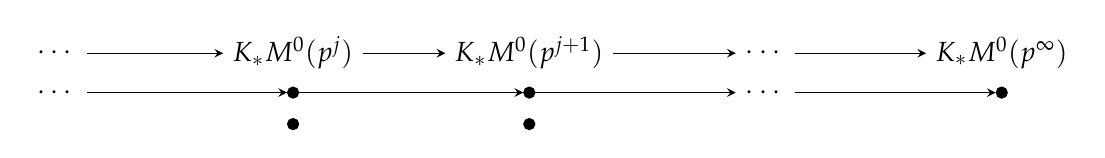
\begin{tikzpicture}[
    baseline=(current bounding box.center),
    normal line/.style={-stealth},
    node distance=3cm,
]
\node (m-1-1) {$\cdots$};
\node[right of=m-1-1] (m-1-2) {$K_* M^0(p^j)$};
\node[right of=m-1-2] (m-1-3) {$K_* M^0(p^{j+1})$};
\node[right of=m-1-3] (m-1-4) {$\cdots$};
\node[right of=m-1-4] (m-1-5) {$K_* M^0(p^\infty)$};
    \path[normal line]
        (m-1-1) edge (m-1-2)
        (m-1-2) edge (m-1-3)
        (m-1-3) edge (m-1-4)
        (m-1-4) edge (m-1-5)
;
\node[below of=m-1-1,node distance=0.5cm] (updot-1) {$\cdots$};
\node[below of=m-1-2,shape=circle,draw,node distance=0.5cm,minimum size=4pt,inner sep=0pt,fill] (updot-2) {};
\node[below of=m-1-2,shape=circle,draw,node distance=0.9cm,minimum size=4pt,inner sep=0pt,fill] (downdot-2) {};
\node[below of=m-1-3,shape=circle,draw,node distance=0.5cm,minimum size=4pt,inner sep=0pt,fill] (updot-3) {};
\node[below of=m-1-3,shape=circle,draw,node distance=0.9cm,minimum size=4pt,inner sep=0pt,fill] (downdot-3) {};
\node[below of=m-1-4,node distance=0.5cm] (updot-4) {$\cdots$};
\node[below of=m-1-5,shape=circle,draw,node distance=0.5cm,minimum size=4pt,inner sep=0pt,fill] (updot-5) {};
\path[normal line]
    (updot-1) edge (updot-2)
    (updot-2) edge (updot-3)
    (updot-3) edge (updot-4)
    (updot-4) edge (updot-5);
\end{tikzpicture}
\end{center}
\caption{``Cell diagram'' of $K_* M^0(p^\infty)$.}\label{CellDiagramFigure}
\end{figure}
This suggests a way we can modify this construction: if we insert other maps which are $K$--homology isomorphisms, then we will not harm this proof that the colimit is an invertible spectrum.  We will make use of the following results to furnish ourselves with such maps:

\begin{definition}[{\cite[Definition 1.5.3]{RavenelOrangeBook}}]
A finite spectrum $X$ is said to be of type $d$ when it is $\Gamma$--locally acyclic for all $\Gamma$ of height strictly less than $d$ and $\Gamma$--locally nontrivial for a $\Gamma$ of height exactly $d$.  (In fact, it suffices to check that acyclicity condition for any single $\Gamma$ of height $(d-1)$~\cite[Theorem 2.11]{RavenelLocalizationWRTPeriodic}.)
\end{definition}

\begin{theorem}[{Devinatz--Hopkins--Smith~\cite[Theorem 9]{HopkinsSmith}}]
A $p$--local finite spectrum $X$ is of type $d$ if and only if for $N \gg 0$ there is a map $v: \Susp^N X \to X$ which is an isomorphism in $K_\Gamma$--homology for $\Gamma$ of height $d$ and which induces the zero map in $K_\Gamma$--homology for $\Gamma$ not of height $d$.
\end{theorem}

\begin{lemma}[{Adams~\cite[Lemma 12.5]{AdamsJXIV}}]\label{AdamsSelfMaps}
The spectrum $M^0(p^{j+1})$ is type $1$ and it admits a map \[v_1^{p^j}: M^{2p^j(p-1)}(p^{j+1}) \to M^0(p^{j+1})\] which induces multiplication by $v_1^{p^j}$ in $K(1)$--homology.\footnote{Here $K(1)$ is the close cousin of $K_{\G_m}$ described in \Cref{MinimalSummands}.} Moreover, the following square commutes:
\begin{center}
\begin{tikzcd}
M^{2p^j(p-1)}(p^j) \arrow{r}{\left(v_1^{p^{j-1}}\right)^p} \arrow{d} & M^0(p^j) \arrow{d} \\
M^{2p^j(p-1)}(p^{j+1}) \arrow{r}{v_1^{p^j}} & M^0(p^{j+1}).
\end{tikzcd}
\end{center}
\end{lemma}

Selecting a $p$-adic integer $a_\infty = \sum_{j=0}^\infty c_j p^j$ with $0 \le c_j < p$, one can now construct the system \[\cdots \to M^{-|v_1| a_{j-1}}(p^j) \to M^{-|v_1| a_{j-1}}(p^{j+1}) \xrightarrow{v_1^{p^j c_j}} M^{-|v_1| a_j}(p^{j+1}) \to M^{-|v_1| a_j}(p^{j+2}) \to \cdots.\] We define $\S^{-|v_1|a_\infty}$ to be its colimit.  \Cref{HMSLines} is then sufficient to check that $\S^{-|v_1| a_\infty}$ is $\G_m$--locally invertible, but more is true:
\begin{lemma}[{\cite[Proposition 2.1]{HMS}}]\label{padicPicElements}
The above construction defines an injective continuous homomorphism of groups \[\Z_p \to \Pic(\CatOf{Spectra}_{\G_m}).\]  When $p \ge 3$ (i.e., $p \ne 2$), the cosets of its image are represented by $\S^1, \ldots, \S^{|v_1|}$.  Abstractly, there is an isomorphism \[\Pic(\CatOf{Spectra}_{\G_m}) \cong \Z_p \rtimes \Z/|v_1|. \qed\]
\end{lemma}

\begin{remark}\label{PicardGroupsWeKnow}
This is the most thorough result of this kind that we know presently.  We also know a calculation of $\Pic(\CatOf{Spectra}_{K(d)})$ for $d = 1$ at $p = 2$~\cite[Theorem 3.3]{HMS}, for $d = 2$ at $p \ge 5$~\cite[Theorem 8.1]{BehrensRevisited}, and for $d = 2$ at $p = 3$~\cite[Theorem 1.2]{GHMR}.  We have partial information for $d = 2$ and $n = 2$~\cite[pg.\ 50]{StricklandInterpolate}, and we know essentially nothing for $n \ge 3$ apart from the Hopkins--Gross analysis of the Brown--Comenetz dualizing spectrum~\cite[Theorem 6]{HopkinsGrossAnnouncement} and the analogue of \Cref{padicPicElements} using ``generalized Moore spectra''~\cite[Proposition 5.14]{HopkinsSmith},~\cite[Proposition 9.2-3]{HMS}.
\end{remark}

That $\Pic(\CatOf{Spectra}_{\G_m}) \cong \Z_p$ carries a profinite topology is not an accident; this, too, is found to be an effect internal to algebraic topology.
\begin{lemma}[{\cite[Proposition 14.3.d]{HoveyStrickland}}]
Let $F(I)$ denote the collection of $\Gamma$--local invertible spectra which become (noncanonically) isomorphic to $L_\Gamma \S^0$ after smashing with the generalized Moore spectrum $M_0(v^I)$.  The $F(I)$ form a basis of closed neighborhoods at the identity which upon linear translation endow $\Pic(\CatOf{Spectra}_\Gamma)$ with the structure of a profinite group. \qed
\end{lemma}

This computation of the Picard group pairs well with another classical calculation:
\begin{theorem}[{\cite[Theorem 1.5]{AdamsJXIV}}]\label{UnpretentiousCalculation}
There are isomorphisms \[\pi_s L_{K(1)} \S^0 \cong \begin{cases} \Z_p & \text{when $s = 0$}, \\ \Z_p / (pk) & \text{when $s = k|v_1| - 1$}, \\ 0 & \text{otherwise}. \qed \end{cases}\]
\end{theorem}

\noindent The right--hand side of this formula can be interpreted through the $p$--adic valuations of the Bernoulli numbers --- or, equivalently, through the special negative values of the Riemann $\zeta$--function: \[\mathbb N \xrightarrow{s \mapsto \zeta(1 - s} \Q \xrightarrow{\text{denom}} \Q / \Z_{(p)} \cong \Z / p^\infty.\]  Number theorists have constructed $p$--adic analytic versions of the Riemann $\zeta$--function by interpolating its special values at negative odd integers and have found such constructions to continue to hold interesting number theoretic data~\cite{Iwasawa}.  For our purposes, it is sufficient to note that the $p$--adic valuation of $\zeta^\wedge_p(1-s)$ for a $p$--adic integer $s = k|v_1| - 1$ agrees with that of $1/(pk)$ and is nonnegative otherwise, so that the formula in \Cref{UnpretentiousCalculation} needs no modification.  However, because the variables $s$ and $k$ in the above formula are linked, taking $k$ to be a general $p$--adic integer necessitates that we also take $s$ to be general $p$--adic integer as well.

\begin{corollary}[{Hopkins, see also Strickland~\cite{StricklandInterpolate}}]
Interpolating the homotopy groups $\pi_* L_{\G_m} \S^0$ using the spectra $\S^{-|v_1|a_\infty}$ constructed in \Cref{padicPicElements} agrees with the number theoretic $p$--adic interpolation of $\zeta$.
\end{corollary}
\begin{proof}
Generally, the cofiber sequence \[\S^n \xrightarrow{p^j} \S^n \to M_n(p^j) \to \S^{n+1} \xrightarrow{p^j} \S^{n+1}\] induces a short exact sequence \[0 \leftarrow (\pi_n X) [p^j] \leftarrow [M_n(p^j), X] \leftarrow (\pi_{n+1} X) / p^j \leftarrow 0,\] and the diagram
\begin{center}
\begin{tikzcd}
\S^n \arrow{r}{p^j} \arrow{d}{1} & \S^n \arrow{r} \arrow{d}{p} & M_n(p^j) \arrow{r} \arrow{d} & \S^{n+1} \arrow{r}{p^j} \arrow{d}{1} & \S^{n+1} \arrow{d}{p} \\
\S^n \arrow{r}{p^{j+1}} & \S^n \arrow{r} & M_n(p^{j+1}) \arrow{r} & \S^{n+1} \arrow{r}{p^{j+1}} & \S^{n+1}
\end{tikzcd}
\end{center}
induces the following map of short exact sequences:
\begin{center}
\begin{tikzcd}
0 & \arrow{l} (\pi_n X)[p^j] & {[M_n(p^j), X]} \arrow{l} & \arrow{l} (\pi_{n+1} X) / p^j & \arrow{l} 0 \\
0 & \arrow{l} \arrow{u}{p} (\pi_n X)[p^{j+1}] & {[M_n(p^{j+1}), X]} \arrow{l} \arrow{u} & \arrow{l} \arrow{u}{\text{quotient}} (\pi_{n+1} X) / (p^{j+1}) & \arrow{l} 0.
\end{tikzcd}
\end{center}
This map of short exact sequences interacts with the Adams $v_1$--self--map of \Cref{AdamsSelfMaps} according to the rectangular prism in \Cref{SelfMapFigure}.
\begin{sidewaysfigure}[ht]
\begin{center}
\begin{tikzcd}[column sep=-0.2cm,row sep=1.5cm]
& 0 & & (\pi_n X)[p^j] \arrow{ll} \arrow{ld} \arrow[leftarrow]{dd} & & {[M_n(p^j), X]} \arrow{ll} \arrow{ld} \arrow[leftarrow]{dd} & & (\pi_{n+1} X) / p^j \arrow{ll} \arrow{ld} \arrow[leftarrow]{dd} & & 0 \arrow{ll} \\
0 & & (\pi_{n-|v_1|p^j} X)[p^j] \arrow[leftarrow, crossing over]{rr} \arrow[red, in=182, out=2, leftarrow]{rrrrru}{\alpha_{j-1/j-1}^p} \arrow{ll} & & {[M_{n-|v_1|p^j}(p^j), X]} & & (\pi_{n-|v_1|p^j+1} X) / p^j \arrow[crossing over]{ll} & & 0 \arrow[crossing over]{ll} \\
& 0 & & (\pi_n X)[p^{j+1}] \arrow{ll} \arrow{ld} & & {[M_n(p^{j+1}), X]} \arrow{ll} \arrow{ld} & & (\pi_{n+1} X) / p^{j+1} \arrow{ll} \arrow{ld} \arrow[red, in=2, out=182]{llllld}{\alpha_{j/j}} & & 0 \arrow{ll} \\
0 & & (\pi_{n-|v_1|p^j} X)[p^{j+1}] \arrow{ll} \arrow[crossing over]{uu} & & {[M_{n-|v_1|p^j}(p^{j+1}), X]} \arrow[crossing over]{uu} \arrow{ll} & & (\pi_{n-|v_1|p^j+1} X) / p^{j+1} \arrow{ll} \arrow[crossing over]{uu} & & 0. \arrow{ll}
\end{tikzcd}
\end{center}
\caption{Interaction of Adams's $v_1$--self--maps with Moore spectra of different indices.}
\label{SelfMapFigure}
\end{sidewaysfigure}
The result follows immediately from the construction of $\S^{-|v_1| a_\infty}$.
%\todo{Actually check that this is sufficient. What about the $v_1$--self--maps?}
\end{proof}

\begin{remark}
We caution the reader that the behavior of the Picard--graded homotopy of the $\Gamma$--local sphere for $\operatorname{ht}(\Gamma) > 1$ is considerably more strangely (i.e., poorly) behaved than that of the $\G_m$--local sphere.  Hovey and Strickland prove a partial ``continuity'' result~\cite[Proposition 14.6]{HoveyStrickland} but also provide details on the remaining bad behavior~\cite[Theorem 15.1]{HoveyStrickland}.  The punchline of the bad news is as follows: take $\Gamma$ to be of height at least $2$, and define $F$ to be the set \[F := \{\lambda \in \Pic(\CatOf{Spectra}_\Gamma) : |\pi_\lambda L_{\Gamma} M^0(p)| < \infty\}.\] Then there is a nonempty open $U$ for which $U \cap F$ is Haar--negligible.  Nonetheless, all but finitely many of the standard spheres belong to $F$ --- a curious situation.
\end{remark}

\begin{remark}
Having set up some of the groundwork of chromatic homotopy theory, we pause to make a remark on the philosophy of the rest of this document.  The other homotopical context in which Picard--graded homotopy groups have taken central relevance is equivariant homotopy theory, which concerns itself with spaces and spectra with a suitable notion of a ``$G$--action'', $G$ a compact Lie group.  The notion of ``$G$--action'' turns out to be somewhat complex, and the correct notion enjoys a notion of cellular approximation, where the cells are formed as follows: for a $G$--representation $V$ we form the representation sphere $S^V$ by compactifying $V$ with a single point at $\infty$.  Cellular approximation then states that any map of $G$--spaces can be $G$--equivariantly weakly replaced by a map of ``$G$--CW--complex'', which are suitably built from the spheres $S^V$ as $V$ ranges.

The analogous construction in chromatic homotopy theory has not appeared before. Although Picard--graded phenomena in the $\Gamma$--local category have been studied, ``Picard--cellular'' constructions have escaped attention.  The primary goal of the remainder of the present work is to construct and study a certain Picard--cellular filtration of $\Gamma$--localized Eilenberg--Mac Lane spaces.
\end{remark}



\end{document}
